\documentclass[11pt,b5paper,oneside,titlepage]{book}
\usepackage{amsmath}
\usepackage{amsfonts}
\usepackage{amssymb}
\usepackage{textcomp}
\usepackage{wasysym}

\usepackage[english, main=bahasa]{babel} % paket bahasa indonesia
\usepackage[T1]{fontenc}
\usepackage[utf8]{inputenc}
\usepackage{libertine} % font Linux Libertine

% membuat index
\usepackage{imakeidx}
\makeindex

\usepackage{minitoc} % paket TOC pada setiap chapter
\usepackage{xcolor} % paket warna
\usepackage{fancyvrb,newverbs}

%----------------------------
% membuat enviroment baru berupa verbatin untuk hasil compile dari setiap
% listing program yang di buat
%------------------------------------------------
\usepackage{verbatim}

\definecolor{cverbbg}{gray}{0.93}

\newenvironment{lcverbatim}
{\SaveVerbatim{cverb}}
{\endSaveVerbatim
	\flushleft\fboxrule=0pt\fboxsep=.5em
	\colorbox{cverbbg}{%
		\makebox[\dimexpr\linewidth-2\fboxsep][l]{\BUseVerbatim{cverb}}%
	}
	\endflushleft
}
%---------------------------
% membuat itemize bulat menjadi checkmark
\usepackage{pifont}
\renewcommand\labelitemi{\ding{52}}


%-----------------------------------------------------
% membuat sebuah label pada hsil output pdf yang dibuat dengan hasil
% asumsi berikut ini
% 1. warna ref, pageref dan TOC berwarna hitam (black)[linkcolor=black]
% 2. warna hyperlink dan url berwarna biru (blue)[urlcolor=blue]
% 3. meta data output pdf adalah:
%	- title = Belajar C++ dengan Qt Creator
%	- Author Nur Wachid
%	- subjek dan Keyword = C++ Qt Creator
%----------------------------------------------------------------------	
\usepackage[pdfpagelabels,colorlinks=true, linkcolor=black, urlcolor=blue]{hyperref}
\hypersetup{
	pdftitle=Belajar C++ dengan Qt Creator ,
	pdfauthor=Nur Wachid,
	pdfsubject=C++ Qt Creator,
	pdfkeywords=C++ Qt Creator,
	bookmarksnumbered=true,     
	bookmarksopen=true,         
	bookmarksopenlevel=1,       
	colorlinks=true,            
	pdfstartview=Fit,           
	pdfpagemode=UseOutlines,    % this is the option you were lookin for
	pdfpagelayout=TwoPageRight
}
%-------------------------------------------------------------

% setting indent pada setiap pargraf sepanjang 1cm
\usepackage{parskip}
\setlength{\parindent}{1cm}
%---------------------------------------
\usepackage{hypcap}
\usepackage{sidecap}
\usepackage{booktabs}
\usepackage[fleqn,tbtags]{mathtools}
\usepackage{longtable}

\usepackage[overlay]{textpos}
\usepackage{wallpaper}
\usepackage{graphicx}
\graphicspath{ {../manuscript/images/} }
%----------------------------------------------
% definisi warna dengan paket dari xcolor
%-----------------------------

\definecolor{bluekeywords}{rgb}{0.13,0.13,1}
\definecolor{bluecomments}{rgb}{0,0,.6}
\definecolor{redstrings}{rgb}{0.9,0,0.9}
\definecolor{greenidentifier}{rgb}{0,.6,0}
\definecolor{keyyellow}{cmyk}{0,0,.8,.3}
\definecolor{cyan}{rgb}{0,0.9,0.9}
\definecolor{orange}{RGB}{255,127,0}
\definecolor{aliceblue}{rgb}{0.94, 0.97, 1.0}
\definecolor{maroon}{rgb}{0.69,0.19,0.38}
\definecolor{darkolivegreen}{rgb}{0.33,0.42,0.18}
%------------------------------------------------------------------------------------
% paket listing digunakan untuk membuat sintaks highliter pada source kode yang di sisipkan
\usepackage{listings}
\lstset{breaklines=true,
	morekeywords={foreach, argc, argv},
%	backgroundcolor=\color{black},
%frame=shadowbox,
	showstringspaces=false,
	basicstyle=\small\ttfamily,
	 numberstyle=\tiny,
	commentstyle=\color{gray},
	keywordstyle=\color{bluekeywords},
	stringstyle=\color{redstrings},
	identifierstyle =\color{greenidentifier},
	basicstyle=\ttfamily,
	numbers=left,
	emph={QDebug,iostream,QtCore,QCoreApplication,QtSql,QtDebug,string,QDomDocument,algorithm,QTextStream,QFile,QDomElement,QDomText,QDataStream,QList,QColor, QDir, QFileInfo},
	 emphstyle=\color{keyyellow},
	emph={[2]dir, isFile,  isDir, isSymLink,absoluteDir,  exists,  isHidden, isReadable, isWritable, isExecutable,  fileName},
	emphstyle={[2]\color{cyan}}
	 }

% meananbahkan listing xml ke dalam dokumen
%------------------------------------------
\lstdefinelanguage{XML}
{
  basicstyle=\small\footnotesize,
  morestring=[b]",
  moredelim=[s][\bfseries\color{maroon}]{<}{\ },
  moredelim=[s][\bfseries\color{maroon}]{</}{>},
  moredelim=[l][\bfseries\color{maroon}]{/>},
  moredelim=[l][\bfseries\color{maroon}]{>},
  morecomment=[s]{<?}{?>},
  morecomment=[s]{<!--}{-->},
  commentstyle=\color{darkolivegreen},
  stringstyle=\color{blue},
  identifierstyle=\color{red}
}
%---------------------------------------------
% ubah listing menjadi contoh
\renewcommand{\lstlistingname}{Contoh}% Listing -> Contoh
\renewcommand{\lstlistlistingname}{Daftar \lstlistingname}% List of Listings -> List of Algorithms
%----------------------------------------------

%-----------------------------------------
% format judul(chapter)
%----------------------------------------------
\usepackage{titlesec}
%\renewcommand{\thechapter}{\Roman{chapter}}
\titleformat{\chapter}[display]
{\bfseries\Large}
{\filleft\MakeUppercase{\chaptertitlename} \Huge\thechapter}
{4ex}
{\titlerule
	\vspace{2ex}%
	\filright}
[\vspace{2ex}%
\titlerule]

%---------------------------------------------------------
% Format Header dan Footer
% 1. Seting Font pada setiap chapter
% 2. Setting font pada setiap section
% 3. Setting font pada nomor halaman di bagian header
% 4. Mencetak nama section terdekat pada bagian sisi sebelah kiri halaman di setiap halaman ganjil
% 5. Mencetak nama section terdekat pada bagian sisi sebelah kanan halaman di setiap halaman genap
% 6. Mengatur lebar garis pada setiap halaman di bawah header selebar 1,5 pt
% 7. 
% 8. menghapus garis pada bagian footer
% 9. judul pada bagian kanan footer
% 10. gambar logo qt pada sisi kiri footer
%-------------------------------------
\usepackage{fancyhdr}
\pagestyle{fancy}
\renewcommand{\chaptermark}[1]{\markboth{\sffamily\normalsize\bfseries\chaptername\ \thechapter.\ #1}{}} % [1]
\renewcommand{\sectionmark}[1]{\markright{\sffamily\normalsize\thesection\hspace{5pt}#1}{}} % [2]
\fancyhf{} \fancyhead[LE,RO]{\sffamily\normalsize\thepage} % [3]
\fancyhead[LO]{\rightmark} % [4]
\fancyhead[RE]{\leftmark} % [5]
\renewcommand{\headrulewidth}{1.5pt} % [6]
\addtolength{\headheight}{2.5pt} % [7] Increase the spacing around the header slightly
\renewcommand{\footrulewidth}{0.5pt} %[8] Removes the rule in the footer
\fancypagestyle{plain}{\fancyhead{}\renewcommand{\headrulewidth}{0pt}} % [9] Style for when a plain pagestyle is specified
\rfoot{Belajar C++ dengan Qt Creator}% [10]
\lfoot{
\includegraphics{logo-qt}} % [11]

%-----------------------------------------
% Menhapus header pada halaman ganjil yang kosong pada akhir chapter
%-----------------------------------------
\makeatletter
\renewcommand{\cleardoublepage}{
	\clearpage\ifodd\c@page\else
	\hbox{}
	\vspace*{\fill}
	\thispagestyle{empty}
	\newpage
	\fi}

%---------------------------------------------
% Paket buat gambar
%------------------------------------------
\usepackage{tikz}
\usetikzlibrary{shapes,arrows}
% Define block styles
	\tikzstyle{decision} = [diamond, draw, fill=blue!20, text width=4.5em, text badly centered, node distance=3cm, inner sep=0pt]
	\tikzstyle{block} = [rectangle, draw, fill=yellow!20, text width=5em, text centered, rounded corners, minimum height=3em]
	\tikzstyle{bloke} = [rectangle, draw, fill=blue!20, text width=4em, text centered, rounded corners, minimum height=2em]
	\tikzstyle{bloke} = [rectangle, draw, fill=blue!20, text width=5em, text centered, rounded corners, minimum height=2em]
	\tikzstyle{blok} = [rectangle, draw, fill=yellow!20, text width=8em, text centered, rounded corners, minimum height=2em]
	\tikzstyle{line} = [draw, -latex']
	\tikzstyle{cloud} = [draw, ellipse,fill=red!20, node distance=3cm,	minimum height=2em]
	\tikzstyle{kotak} = [rectangle, draw, fill=green!20, text width=8em, text centered, rounded corners, minimum height=7em]
	\tikzstyle{ling} =  [draw, circle,fill=red!20, node distance=3cm, minimum height=1em]
	\tikzstyle{titik} =  [draw]

%------------------------------------------
% Efek shadow untuk gambar 

\usetikzlibrary{shadows,calc}

% code adapted from http://tex.stackexchange.com/a/11483/3954

% some parameters for customization
\def\shadowshift{3pt,-3pt}
\def\shadowradius{6pt}

\colorlet{innercolor}{black!60}
\colorlet{outercolor}{gray!05}

% this draws a shadow under a rectangle node
\newcommand\drawshadow[1]{
    \begin{pgfonlayer}{shadow}
        \shade[outercolor,inner color=innercolor,outer color=outercolor] ($(#1.south west)+(\shadowshift)+(\shadowradius/2,\shadowradius/2)$) circle (\shadowradius);
        \shade[outercolor,inner color=innercolor,outer color=outercolor] ($(#1.north west)+(\shadowshift)+(\shadowradius/2,-\shadowradius/2)$) circle (\shadowradius);
        \shade[outercolor,inner color=innercolor,outer color=outercolor] ($(#1.south east)+(\shadowshift)+(-\shadowradius/2,\shadowradius/2)$) circle (\shadowradius);
        \shade[outercolor,inner color=innercolor,outer color=outercolor] ($(#1.north east)+(\shadowshift)+(-\shadowradius/2,-\shadowradius/2)$) circle (\shadowradius);
        \shade[top color=innercolor,bottom color=outercolor] ($(#1.south west)+(\shadowshift)+(\shadowradius/2,-\shadowradius/2)$) rectangle ($(#1.south east)+(\shadowshift)+(-\shadowradius/2,\shadowradius/2)$);
        \shade[left color=innercolor,right color=outercolor] ($(#1.south east)+(\shadowshift)+(-\shadowradius/2,\shadowradius/2)$) rectangle ($(#1.north east)+(\shadowshift)+(\shadowradius/2,-\shadowradius/2)$);
        \shade[bottom color=innercolor,top color=outercolor] ($(#1.north west)+(\shadowshift)+(\shadowradius/2,-\shadowradius/2)$) rectangle ($(#1.north east)+(\shadowshift)+(-\shadowradius/2,\shadowradius/2)$);
        \shade[outercolor,right color=innercolor,left color=outercolor] ($(#1.south west)+(\shadowshift)+(-\shadowradius/2,\shadowradius/2)$) rectangle ($(#1.north west)+(\shadowshift)+(\shadowradius/2,-\shadowradius/2)$);
        \filldraw ($(#1.south west)+(\shadowshift)+(\shadowradius/2,\shadowradius/2)$) rectangle ($(#1.north east)+(\shadowshift)-(\shadowradius/2,\shadowradius/2)$);
    \end{pgfonlayer}
}

% create a shadow layer, so that we don't need to worry about overdrawing other things
\pgfdeclarelayer{shadow} 
\pgfsetlayers{shadow,main}


\newcommand\shadowimage[2][]{%
\begin{tikzpicture}
\node[anchor=south west,inner sep=0] (image) at (0,0) {\includegraphics[#1]{#2}};
\drawshadow{image}
\end{tikzpicture}}

%-------------------------------------------
% Isi konten dari bagian dasar, OOP, interface, widget dan Library
% memuat  bab
\begin{document}
	\dominitoc 
%	\pagecolor{aliceblue}
%----------------------------------------------------------------------------------------
%	TITLE PAGE
%----------------------------------------------------------------------------------------
	\begingroup  
	\thispagestyle{empty}
	\begin{textblock*}{297mm}(0mm,0mm)
		\ThisTileWallPaper{\paperwidth}{\paperheight}{cover}
	\end{textblock*}
	\endgroup
	\title{Belajar C++ dengan Qt Creator}
	\author{Nur Wachid}
	\cleardoublepage
	\frontmatter

	\begingroup
	\parskip \baselineskip
	\thispagestyle{empty}

\noindent 
\includegraphics[width=0.2\textwidth]{cc-by-nc}

\noindent \textcopyright{} 2016 Nur Wachid \\
	All rights reserved.
	
	Buku ini boleh digandakan atau didistribusikan dengan
	seizin penulis atau mencantumkan \emph{credit} kepada
	website penulis atau email penulis. Tetapi pendistribusian
	buku ini tidak boleh untuk kepentingan komersial.
	
\noindent Penulis: Nur Wachid \\
	Website: \url{http://turahe.github.io}  \\
	Email: \texttt{wachid  (at) outlook dot com} \\
	\phone  0858 7984 5219
	
	\chapter{Tentang Penulis}
	\section*{Tentang Penulis}

\subsection*{Nur Wachid}

\textbf{Head of Software Engineering} \\
PT. Lingkar Kreasi Teknologi \\
Tangerang, Indonesia

\vspace{0.5cm}

\begin{quote}
\textit{Experienced programmer with a strong background in software development and a passion for problem-solving. Proficient in designing, coding, testing, and maintaining software applications. Adept at collaborating with cross-functional teams to deliver high-quality solutions. Specialized in web development and mobile app development.}
\end{quote}

\subsection*{Profil Profesional}

Nur Wachid adalah seorang profesional di bidang software engineering dengan pengalaman lebih dari 7 tahun dalam pengembangan aplikasi. Saat ini menjabat sebagai \textbf{Head of Software Engineering} di PT. Lingkar Kreasi Teknologi, memimpin tim pengembang dalam menciptakan solusi teknologi yang inovatif.

\subsection*{Keahlian Utama}

\begin{itemize}
\item \textbf{Software Development} - Desain, pengembangan, testing, dan maintenance aplikasi
\item \textbf{Web Development} - Pengembangan aplikasi web modern dan responsif
\item \textbf{Mobile App Development} - Pengembangan aplikasi mobile cross-platform
\item \textbf{Enterprise Resource Planning (ERP)} - Sistem manajemen perusahaan
\item \textbf{Data Pipelines} - Otomatisasi dan pengelolaan data
\item \textbf{Machine Learning} - Implementasi AI dan machine learning
\item \textbf{DevOps Engineering} - Infrastructure as Code, CI/CD, Containerization
\item \textbf{Backend Development} - RESTful API, Database optimization, Security
\end{itemize}

\subsection*{Pengalaman Profesional}

\subsubsection*{Head of Software Engineering @ PT. Lingkar Kreasi Teknologi}
\textit{Agustus 2022 - Desember 2024 | Tangerang, Indonesia}

\begin{itemize}
\item Memimpin tim pengembang dengan meningkatkan produktivitas tim sebesar 20\%
\item Mengelola proyek kompleks dengan tingkat kepuasan klien 95\%
\item Merancang arsitektur inovatif yang mengurangi biaya server 30\% dengan peningkatan traffic 200\%
\item Membimbing developer junior dan meningkatkan keterampilan teknis tim
\item Menerapkan proses code review yang mengurangi bug kritis sebesar 40\%
\end{itemize}

\subsubsection*{VP DevOps Engineer @ PT. Lingkar Kreasi}
\textit{November 2019 - Agustus 2022 | Bandung, Indonesia}

\begin{itemize}
\item Merancang pipeline deployment otomatis yang mengurangi waktu deployment dari hari menjadi menit
\item Menerapkan Infrastructure as Code menggunakan Terraform dan AWS CloudFormation
\item Mengarsitektur infrastruktur high availability dengan uptime 99.99\%
\item Mengelola container menggunakan Kubernetes dan Docker Swarm
\item Menetapkan CI/CD pipeline yang mengurangi kegagalan deployment 50\%
\end{itemize}

\subsubsection*{Backend Developer @ PT. Rakhasa Artha Wisesa}
\textit{Februari 2021 - November 2022 | Jakarta, Indonesia}

\begin{itemize}
\item Meningkatkan performa database query sebesar 40\%
\item Menerapkan keamanan tingkat lanjut dengan zero security breach dalam 2 tahun
\item Mengembangkan RESTful API yang mengurangi response time 50\%
\item Mengintegrasikan payment gateway yang meningkatkan transaksi berhasil 20\%
\end{itemize}

\subsubsection*{Project Lead Developer @ PT. Lingkar Kreasi}
\textit{November 2018 - November 2019 | Bandung, Indonesia}

\begin{itemize}
\item Memimpin tim cross-functional dengan tingkat penyelesaian proyek tepat waktu 95\%
\item Mempertahankan tingkat kepuasan klien 90\% atau lebih tinggi
\item Mengidentifikasi dan mitigasi risiko proyek secara proaktif
\item Mengelola anggaran proyek dengan efisiensi 15\%
\end{itemize}

\subsubsection*{Web Developer @ PT Danadipa Central Niaga}
\textit{November 2017 - November 2018 | Yogyakarta, Indonesia}

\begin{itemize}
\item Mengembangkan dan meluncurkan website skala besar untuk klien
\item Mengoptimalkan performa website untuk meningkatkan user experience
\item Menerapkan keamanan website dengan enkripsi data dan proteksi cyberattack
\end{itemize}

\subsection*{Fokus Saat Ini}

Saat ini Nur Wachid fokus pada pengembangan:
\begin{itemize}
\item \textbf{Enterprise Resource Planning (ERP)} - Sistem manajemen perusahaan terintegrasi
\item \textbf{Data Pipelines} - Otomatisasi pengelolaan dan analisis data
\item \textbf{Machine Learning} - Implementasi AI untuk optimasi bisnis
\item \textbf{Open Source} - Kontribusi aktif dalam proyek open source
\end{itemize}

\subsection*{Kontribusi Pendidikan}

Nur Wachid aktif menulis buku dalam bidang:
\begin{itemize}
\item \textbf{Pemrograman} - Buku panduan C++ dan Qt untuk pemula
\item \textbf{Data Science} - Analisis data dan machine learning
\item \textbf{Teknik Elektro} - Bidang keahlian akademis
\end{itemize}

\subsection*{Filosofi Pengembangan}

\begin{quote}
\textit{"I am always looking to learn new things. I am a strong advocate for open source and I am always interested in working on new projects with new people."}
\end{quote}

\subsection*{Kontak}

\begin{itemize}
\item \textbf{Email}: [Email tersedia di profil]
\item \textbf{GitHub}: [GitHub tersedia di profil]
\item \textbf{LinkedIn}: [LinkedIn tersedia di profil]
\item \textbf{Website}: \url{https://www.wach.id}
\item \textbf{WhatsApp}: [WhatsApp tersedia di profil]
\end{itemize}

\vspace{1cm}

\begin{center}
\textit{--- Penulis buku "Belajar C++ dengan Qt Creator" ---}
\end{center}
	
	\endgroup
	\tableofcontents
	\lstlistoflistings

	\clearpage
	\newpage
	\chapter{Prakata}
	Bahasa pemrograman C/C++ merupakan bahasa yang popular didalam
pengajaran pada computer sains maupun pada kalangan programmer yang
mengembangkan system software maupun aplikasi.

Bahasa C/C++ sifatnya portable, karena compilernya tersedia hampir pada
semua arsitektur computer maupun system operasi, sehingga investasi
waktu dan tenaga yang anda lakukan dalam mempelajari bahasa pemrograman
ini memiliki nilai strategis yang sangat menjanjikan.

Bahasa C/C++ merupakan bahasa yang sangat ketat dalam pemakaian type
data maupun penulisannya yang case sensitif, hal ini berarti programmer
di tuntut kedisiplinannya dalam penulisan program.

Sesuatu fasilitas yang tersedia dalam C/C++ yang tidak ditemukan pada
bahasa pemrogaman lainnya adalah pointer, dengan pemanfaatan pointer
programmer dapat melakukan manipulasi memori secara langsung.

Dewasa ini beberapa bahasa yang memiliki syntax penulisan yang
menyerupai C/C++ adalah Java, Javascript dan PHP, yang artinya bahwa
kemampuan pemrograman dengan C/C++ akan mempermudah anda untuk
mempelajari bahasa modern seperti Java maupun C\# (dibaca C sharp).

Akhirnya penulis mengucapkan selamat belajar dan semoga buku ini dapat
memberi manfaat yang sebesarnya dalam pembelajaran mata kuliah C/C++
Programming.

\section*{Struktur buku ini}

\begin{description}
	\item[Bab 1. Mukadimah] Pada bab ini akan di perkenalkan mengenai
	 bahasa C++, mengenal Qt Creator, teknologi User Interface yang 
	 digunakan, Instalasi dan Struktur program C++ pada Qt Creator secara umum 
	\item[Bab 2. tipe data, identifier, Operator dan Control Flow] 
	pada bab ini akan di bahas tuntas mengenai apa itu tipe data C++, 
	Variabel dan konsanta, Statement, Operator dan Control Statement.
	\item[Bab 3. Array dan String] Pada bab ini akan di perkenalkan 
	macam-macam array dari array 1 dimensi sampai dengan array 
	multidimesi dan String berupa penggunaan string di dalam bahasa C++.
	\item[Bab 4. Fungsi] Pada bab ini akan mempelari tentang konsep dasar
	fungsi cara mendefinisikan fungsi dan medeklarasikanya, Hasil balik
	fungsi serta mempelajari ruang lingkup variabel dan pengiriman parameter

\end{description}
	\newpage
	\cleardoublepage
	\mainmatter

%---------------------------------------------
% Dasar dari pemrograman C++ yakni mengenai
% 1 mukadimah, tipe data, indetifier, operator  control flow
%	array, string, fungsi, pointer, rekursif
%----------------------------------------------	
\part{Dasar}
%-------------------------------------------------
\begingroup
\thispagestyle{empty}
\vspace*{5cm}
\par\normalfont\fontsize{25}{25}\sffamily\selectfont

\textcolor{blue}{PUBLIC} \textcolor{green}{CLASS} \textcolor{red}{LOVE} \textcolor{orange}{\{}

\textcolor{gray}{SYSTEM.OUT.PRINT}\textcolor{orange}{\{}ILOVEYOU \textcolor{orange}{\}}

\textcolor{gray}{RETURN} \textcolor{red}{TRUE} \textcolor{orange}{\{}LOVE \textcolor{orange}{\}}

\textcolor{orange}{\}}

\endgroup

%------------------------------------------------	
	\chapter{Mukadimah}\label{mukadimah}
	\textbf{Agenda}

Pada chapter ini kita akan membahas mengenai bahasa C dan Qt Cretor 
seperi berikut ini

\minitoc

\section{Pengenalan Bahasa C++}\label{pengenalan-bahasa-cpp}



Bahasa C merupakan bahasa pemrograman tingkat menengah. Pada tahun 1972
bahasa C pertama kali dirancang oleh \index{Dennis M Ritchie}
\href{https://id.wikipedia.org/wiki/Dennis_Ritchie}{Dennis M Ritchie}\footnote{https://id.wikipedia.org/wiki/Dennis\_Ritchie}{Dennis M Ritchie} di
Bell aboratories. Kemudian tahun 1978 Dennis dan\index{Brian W. Kernighan} 
\href{https://id.wikipedia.org/wiki/Brian_Kernighan}{Brian W. Kernighan}\footnote{https://id.wikipedia.org/wiki/Brian\_Kernighan}{Brian W. Kernighan}
mempublikasikan bahasa C melalui \index{The C
	Programming Language}
\href{https://id.wikipedia.org/wiki/The_C_Programming_Language}{The C
Programming Language}\footnote{https://id.wikipedia.org/wiki/The\_C\_Programming\_Language} sehingga bahasa C dikenal banyak orang.
Selanjutnya pada tahun 1989, akhirnya bahasa C distandardisasi \index{ANSI}
\href{https://id.wikipedia.org/wiki/ANSI_C}{ANSI}\footnote{https://id.wikipedia.org/wiki/ANSI\_C} (American National
Standard Institute) sehingga bahasa C menjadi bahasa pemrograman standar
hingga saat ini dan bisa dibuat kompilernya pada beberapa platform yang
berbeda-beda.

Bahasa C dikatakan sebagai bahasa pemrograman terstruktur, fungsional
karena strukturnya menggunakan fungsi-fungsi sebagai program-program
bagian (subroutine/ module). Fungsifungsi selain fungsi utama disebut
subroutine/ module dan ditulis setelah fungsi utama (main) atau
diletakkan pada file pustaka (library). Jika fungsi-fungsi diletakkan
pada file pustaka dan akan dipakai disuatu program, maka nama file
header-nya harus dilibatkan dalam program menggunakan preprocessor
directive \texttt{\#include}.

Kemudian bahasa C dikembangkan oleh Bjarne Stroustrup at Bell Labs
menjadi bahasa C++. Pada bulan Oktober 1985 munculah buku \emph{The C++
Programming Language} yang membahas tentang bahasa pemrograman itu
langsung dari penciptanya sendiri. Bahasa C++ mengalami dua tahap
evolusi.

\begin{dingautolist}{192}

\item
  Pertama, dirilis oleh
  \href{https://id.wikipedia.org/wiki/Bell_Laboratories}{AT\&T
  Laboratories}\footnote{Bell Laboratories (juga dikenal dengan nama Bell Labs dan sebelumnya dengan nama AT\&T Bell Laboratories dan Bell Telephone Laboratories) adalah bagian dari organisasi riset dan pengembangan dari Alcatel-Lucent dan sebelumnya dari United States Bell System.}, dinamakan
  \href{https://en.wikipedia.org/wiki/Cfront}{cfront}\footnote{https://en.wikipedia.org/wiki/Cfront}. C++ versi ini
  hanya berupa kompiler yang menterjemahkan bahasa C++ menjadi bahasa C
  untuk dieksekusi
\item
  Kedua, \href{https://en.wikipedia.org/wiki/Borland}{Borland
  International Inc}\footnote{Borland Software Corporation adalah sebuah perusahaan perangkat lunak komputer yang berkantor pusat di Austin, Texas. Perusahaan ini didirikan pada tahun 1983 oleh Niels Jensen, Ole Henriksen, Mogens Glad dan Philippe Kahn.}. mengembangkan kompiler C++ menjadi sebuah kompiler
  yang mampu mengubah C++ langsung menjadi bahasa mesin (assembly).
  Tahun1990, C++ mulai diarahkan ke pengembangan
  \href{https://id.wikipedia.org/wiki/Pemrograman_berorientasi_objek}{Pemrograman
  Berorientasi Obyek}\footnote{OOP (Object Oriented Programming) adalah suatu metode pemrograman yang berorientasi kepada objek. Tujuan dari OOP diciptakan adalah untuk mempermudah pengembangan program dengan cara mengikuti model yang telah ada di kehidupan sehari-hari.}.

\end{dingautolist}

Beberapa keunggulan C++ dibandingkan dengan bahasa C adalah sebagai
berikut.

\begin{description}

\item[Object-oriented programming]
Bahasa pemrograman ini sangat mendukung pemrograman berorientasi obyek
yang melihat permasalahan secara obyek dan bukan prosedural.
\item[Portability]
Kita dapat mengkompilasi C++ kode yang sama di hampir semua jenis
komputer dan sistem operasi tanpa membuat perubahan apapun. C++ adalah
bahasa pemrograman yang paling sering digunakan di dunia.
\item[Brevity]
Karena bahasa C++ merupakan bahasa tingkat tinggi, maka bahasa yang
ditulis dengan bahasa C++ termasuk ringkas dan pendek dibandingkan
bahasa-bahasa sejamannya pada waktu itu.Bahasa C++ termasuk bahasa
pemrograman tua yang sudah mendukung berbagai macam kata kunci yang
mampu menyingkat proses penulisan kode program.
\item[Modular programming\footnote{pemrograman modular adalah mengelompokkan fungsi-fungsi utama kedalam sebuah modul, dimana tiap-tiap modul memiliki datanya masing-masing dan mampu mengolah datanya sendiri. Modul-modul ini yang akan digunakan dalam program.}]
Tubuh program pada bahasa C++ dapat terdiri dari beberapa file source
code yang disusun secara terpisah dan kemudian dihubungkan secara
bersama-sama. Kemampuan ini jelas menghemat waktu karena tidak perlu
mengkompilasi ulang aplikasi yang lengkap ketika membuat satu perubahan,
tetapi hanya file yang berisi perubahan itu saja. Selain itu,
karakteristik ini memungkinkan kita untuk menghubungkan kode C++ dengan
kode yang dibuat oleh bahasa lain, seperti bahasa Assembly dan C dan
dapat digunakan kembali (reuseable).
\item[C Compatibility]
C++ sangat backward compatible dengan bahasa C, sehingga aplikasi / kode
program yang ditulis dengan bahasa C dapat digabungkan dengan bahasa C++
dengan sangat mudah, bahkan hampir tidak perlu mengubah kodenya.
\item[Speed]
Kode yang dihasilkan dari kompilasi C++ sangat efisien, karena C++
mendukung prinsip dualitas bahwa dia mendukung bahasa tingkat tinggi dan
bahasa tingkat rendah sehingga dapat mengurangi ukuran hasil kompiliasi
dari bahasa itu.
\end{description}

\section{Pengantar Qt Creator}\label{pengantar-qt-creator}

Qt Creator merupakan cross-platform C++ integrated development
environment yang merupakan bagian dari Qt SDK \index{Qt SDK}. Qt Creator mempunyai
debugger dalam bentuk visual dan layout GUI \index{GUI} serta tempat perancangan
form. Teks editornya mempunyai fasilitas syntax highlighting dan
autocompletion. Qt Creator menggunakan compiler C++ dari kumpulan
compiler \index{GNU}GNU pada \index{Linux}Linux dan \index{FreeBSD}FreeBSD. Pada Windows \index{Windows} Qt Creator dapat
menggunakan MinGW\footnote{minGW adalah salah satu aplikasi yng
  digunakan untuk mengkompile bahasa C agar dapat dipahami oleh bahasa
  mesin (asembler) pada komputer. Aplikasi ini dapat di unduh secara
  gratis.} atau
\href{https://id.wikipedia.org/wiki/Microsoft_Visual_Studio_Express}{MSVC}\footnote{sebuah perangkat lunak lengkap (suite) yang dapat digunakan untuk melakukan pengembangan aplikasi, baik itu aplikasi bisnis, aplikasi personal, ataupun komponen aplikasinya, dalam bentuk aplikasi console, aplikasi Windows, ataupun aplikasi Web. Visual Studio mencakup kompiler, SDK, Integrated Development Environment (IDE), dan dokumentasi (umumnya berupa MSDN Library). Kompiler yang dimasukkan ke dalam paket Visual Studio antara lain Visual C++, Visual C\#, Visual Basic, Visual Basic .NET, Visual InterDev, Visual J++, Visual J\#, Visual FoxPro, dan Visual SourceSafe.}
yang sudah build-in di dalam install.

Project Qt Creator seperti pada gambar \ref{fig:projek-pada-qt-creator}
 menggunakan format cross platform project (.pro)
untuk mengizinkan tim developer untuk share project yang mempunyai
platform-platform yang berbeda-beda dan menggunakan common tool untuk
implementasi dan debugging program. Sebuah project dapat meliputi:

file-file yang digroup secara bersama-sama, langkah-langkah build
program, form-form dan file-file resource, dan pengaturan untuk
menjalankan aplikasi.

Projek dapat dibuat secara manual atau diimport dari file projek yang
sudah ada. Jika projeknya dibuat secara manual, maka sebuah file-file
akan digenerate oleh Qt Creator, tergantung dari tipe file yang
dimiliki. Seperti Jika filenya adalah sebuah GUI application, maka Qt
Creator men-generate sebuah file kosong yang berektensikan \texttt{.ui}
yang akan imodifikasikan melalui Qt Designer\index{Qt Designer}. Qt Creator diinterrasikan
dengan sistem cross-platform untuk mem-build secara automatis: qmaka\index{qmake} dan CMake
\index{CMake}. Projek yang tidak menggunakan qmake atau CMake dapat
diimport-kan, dan Qt Creator dapat meng-ignore sistem build.

\begin{figure}[htbp]
\centering 
\shadowimage[width=8cm]{Capture1-1}
\caption{Projek pada Qt Creator}
\label{fig:projek-pada-qt-creator}
\end{figure}

Editor Qt Creator seperti pada gambar \ref{fig:code-editor}
 mempunyai sebuah code editor yang telah terintegrasi
dengan Qt Designer untuk mendesain dan membangun aplikasi GUI dari 
\index{Qt	widgets}Qt widgets. Karena Qt Creator adalah sebuah 
Integrated Development Enviroment (IDE), maka Qt Creator memisahkan 
antara text editor untuk build dan editor untuk menjalankan (run) 
aplikasi-aplikasi. Qt Creator bukan hanya bisa membaca text file biasa, 
akan tetapi juga bisa membaca file C++ dan bahasa QML\index{QML}.

Keunggulan Code Editor Qt Creator

\begin{dinglist}{52}

\item
  Dapat menulis code dengan format yang benar.
\item
  Mengantisipasikan apa yang akan programer tulis dan code yang komplit.
\item
  Menampilkan baris-baris yang error dan pesan-pesan warning.
\item
  Memandu programer secara semantik untuk menulis classes, functions,
  dan symbols.
\item
  Menyediakan fasilitas bantuan context-sensitive pada classes,
  functions, dan symbols.
\item
  Me-rename symbol-symbol dengan langkah intelligent, sehingga
  simbol-simbol yang lain dengan nama yang sama tidak ter-rename.
\item
  Menampilkan lokasi function, class yang dideklarasikan atau yang
  dipanggil
\end{dinglist}

\begin{figure}[htbp]
\centering
\shadowimage[width=8cm]{Capture1-2}
\label{fig:code-editor}
\caption{ Code Editor}
\end{figure}

\subsection{UI Designer}\label{ui-designer}

Qt Creator menyajikan dua buah editor visual: \index{Qt Designer}
Qt Designer  dan \index{Qt Quick	Designer}Qt Quick
Designer. Qt Designer merupakan sebuah tool untuk mendesain dan
membangun aplikasi GUI dari \index{Qt widgets}Qt widgets. Widgets dan forms yang dibentuk
dengan Qt Designer terintegrasi dengan code program, Qt signals dan
mekanisme slots, sehingga kita dengan mudah memberikan nilai-nilai dan
properti-properti pada pada elemen-elemen grafik. Semua
properti-properti yang diatur pada Qt Designer dapat diubah secara
dinamik melalui/di dalam code.

Qt Quick Designer seperti gambar \ref{fig:gambar-ui-designers}
digunakan untuk membangun secara mudah animasi-animasi
dengan menggunakan sebuah bahasa pemograman yang dikenal dengan
\href{https://en.wikipedia.org/wiki/QML}{Qt Meta-Object Language 
(QML)}\footnote{https://en.wikipedia.org/wiki/QML}.
Dalam QML, sebuah user interface dispesifikasikan sebagai sebuah pohon
(tree) dari objects dengan properti-properti. anda bisa menggunaan teks
editor visual untuk menciptakan items, screens, dan aplikasi, serta
mendefinisikan perubahan action-acton pada komponennya. Dapat digunakan
Qt atau JavaScript untuk mengimplementasikan logika aplikasi.

\begin{figure}[htbp]
\centering
\shadowimage[width=8cm]{Capture1-3}
\caption{Gambar UI Designers}
\label{fig:gambar-ui-designers}
\end{figure}

\subsection{Bahasa yang di dukung}\label{bahasa-yang-di-dukung}

Anda dapat menggunakan code editor menulis code dalam Qt C++ atau bahasa
pemograman QML, javascript bahkan HTML5. Syntax highlighting juga
disajikan untuk banyak bahasa pemograman yang lain.

\subsection{Platform}\label{platform}

Qt Creator men-support untuk membangun dan menjalankan aplikasi-aplikasi
Qt untuk desktop environments (Seperti Windows, Linux, FreeBSD dan Mac
OS) Selain itu juga bisa dijalankan pada mobile devices (seperti
Android, windows 8 dan iOS). Ketika sebuah aplikasi dibangun untuk
mobile device yang bisa mengkoneksi ke Personal Computer (PC), maka Qt
Creator men-generate sebuah package instalasi, menginstall package
tersebut pada device, dan meneksekusikannya.

\subsection{Tools}\label{tools}

Qt Creator diintegrasikan dengan kumpulan tool-tool yang bermanfaat dan
membantu, seperti version control systems dan Qt Simulator. Qt Creator
menggunakan command line client version control system untuk mengakses
repositories (\href{https://git-scm.com/}{Git}\footnote{Git adalah tools 
yang berfungsi sebagai Version Control System (VCS) dan kalau diartikan 
ke bahasa kita artinya sebuah sistem pelacak perubahan pada file.},
\href{https://subversion.apache.org/}{subversion}\footnote{Subversion
(SVN) adalah salah satu version control system popular yang ada. 
SVN mula-mula diciptakan sebagai pengganti CVS, software yang 
popular sebelumnya namun memiliki banyak kelemahan.},
\href{https://www.perforce.com}{Perfoce}\footnote{https://www.perforce.com},
\href{www.nongnu.org/cvs/}{CVS}\footnote{Computer vision syndrome (CVS) adalah suatu keadaan yang terjadi karena terlalu lama memfokuskan mata pada layar komputer. Umumnya penderita akan mengeluhkan nyeri kepala, pusing, penglihatan kabur, nyeri leher, mata merah, penglihatan ganda, sulit memfokuskan mata, bahkan kelelahan.},
\href{https://www.mercurial-scm.org}{Mercurial}\footnote{Mercurial adalah salah satu software revision control yang dikembangkan dengan menggunakan Python, dan tersedia untuk beberapa platform seperti Linux, Windows dan MacOS.  Tidak seperti software revision control lain yang sudah lama dipakai seperti CVS dan SVN, Mercurial menggunakan distributed revision control.  Dengan demikian, tidak ada satu server pusat yang berisi repository source-code (koleksi kode program).  Setiap orang dapat mengambil source code dari sebuah repository, kemudian membuat repository-nya sendiri.}).

\subsection{Debuggers}\label{debuggers}

Qt Creator tidak mempunyai debugger. Qt Creator mempunyai plugin
debugger yang bekerja sebagai interface antara Qt Creator core dan
external native debuggers

Debuggers adalah:

\begin{dinglist}{51}

\item
  GNU Symbolic Debugger (gdb)
\item
  Microsoft Console Debugger (CDB)
\item
  internal Java Script debugger
\end{dinglist}

Dapat menghubungkan mobile devices dengan PC dan memproses debug yang
berjalan pada devices.

\section{Mengenal macam - macam Teknologi User Interface (UI) pada QT}\label{mengenal-macam-macam-teknologi-user-interface-ui-pada-qt}

Interaksi antara pengguna dengan logic software dinamakan User Interface
disingkat dengan UI. UI ini berwujud bisa sebuah window, bisa tombol,
bisa sebuah textarea dan lain sebagainya. Inilah komponen User
Interface. Sebagai seorang programmer (pembuat program aplikasi),
terlebih programmer yang menggunakan Qt, maka anda akan disediakan
beragam UI yang bisa anda pilih sesuai kebutuhan. Ada QtWitget, QtQuick
dan QtWebKit. Ketiganya dapat anda pilih sesuai kebutuhan sebagai UI
progam anda. Ingin tahu bedanya? Mari kita simak.

Sama seperti Visual Studio yang menyediakan beragam Amazing User
Interface tingkat tinggi sampai pengguna bingung memilihnya, Qt
menyediakan tiga UI yang dapat kita gunakan. Anda pun bisa menggabungkan
ketiganya. \smiley

Qt Creator, sebuah Editor Qt adalah contoh dari perpaduan multiple
teknologi UI ini. Coba amati Qt Creator yang selalu anda gunakan
tersebut.

Qt Creator menggunakan teknologi QtWidget sebagai User Interface pada
menu dan kotak dialog nya. Coba perhatikan kembali Welcome Screen dari
Qt Creator, lihat, tampilannya berbeda bukan, bahkan button nya sangat
berbeda dan tidak biasa, ini karena UI untuk Welcome Screen menggunakan
teknologi QtQuick. Lalu dimana letak penggunaan QtWebkit?

Yup, perhatikan Help Documentation nya, wow, ini seperti halaman web
yang menyatu dengan softwarenya bukan? Ya, teknologi QtWebKit digunakan
dalam pembangunan Help Documentation ini.

\subsection{Teknologi User Interface QtQuick}\label{teknologi-user-interface-qtquick}

QtQuick merupakan salah satu Teknologi UI dari Qt yang menggunakan QML
dan JavaScript sebagai penyusun UI nya.Mirip seperti XAML yang
dikembangkan Microsoft , QML merupakan teknologi binding dari Qt yang
memfasilitasi pengguna dengan visual canvas dan rendering engine nya.
Teknologi UI ini sangat cocok sekali untuk Hardware Acceleration seperti
OpenGL pada VGA driver kita.

Jangan salah, bila anda menggunakan QtQuick versi 2, maka memang butuh
OpenGL yang disuport oleh VGA anda. OpenGL sekarang begitu terkenal,
banyak games - games yang mulai menargetkan OpenGL karena begitu
flexibel dan mudah. Tapi sayangnya, OpenGL ini tidak terdapat pada VGA
driver bawaan OS.

Jadi jangan heran, saat anda install ulang komputer (bahkan Windows 8.1
sekalipun) anda akan menemukan bahwa tidak ada OpenGL pada VGA driver
anda. Cara terbaik adalah periksa Motherboard anda dan cari driver VGA
yang sesuai dengan Motherboard anda. Biasanya gratis.

Animation, Transition, Visual Effect, Shader Effect dan lain -- lain
merupakan fasilitas yang dapat anda kembangkan saat menggunakan QtQuick
sebagai User Interface (UI) aplikasi anda.

\subsection{Teknologi User Interface QtWidget}\label{teknologi-user-interface-qtwidget}

QtWidget merupakan tradisional User Interface element yang biasanya
terdapat dalam dekstop environment. Bila anda pengguna linux, maka UI
ini merupakan bagian dari KDE. Tapi jangan salah, QtWidget sangat
dinamis untuk Windows dan Mac OS. Sehingga bila anda menggunakan
QtWidget sebagai UI anda maka tampilannya mirip sekali dengan UI pada OS
anda.

Bila anda pengguna Windows 8.1 seperti saya dengan Amazing Flat
Designnya, maka QtWidget ini menyesuaikan dengan UI OS.

Semua standar komponen untuk aplikasi seperti button, textarea, menu dan
lain -- lain terdapat pada QtWidget ini. Sehingga sangat cocok sekali
untuk anda yang gemar membuat aplikasi tradisional standar.

Bila kita membuat aplikasi dengan QtWidget, maka saat memulai project,
akan muncul pemilihan Base Class, ada tiga yaitu Class QWidget, Class
QMainWindow, dan Class Qdialog.

Perbedaan dari ketiga Base Class di atas adalah berikut ini.

\begin{dingautolist}{192}
\item
  \texttt{*QWidget} merupakan base class untuk semua GUI element pada
  QtWidget User Interface. Coba lah explorasi dan bedakan ketiganya :)
\item
  \texttt{*QDialog} merupakan sebuah window yang biasanya digunakan
  untuk mengejutkan pengguna, seperti saat window dialog muncul ketika
  pengguna harus memasukan input dengan benar atau hal -- hal yang lain,
  tampilan dari Qdialog tidak berbeda dengan Qwidget, anda bisa
  menggunakan salah satu.
\item
  \texttt{*QMainWindow}, nah, ini adalah sebuah class yang sangat unik,
  karena menggunakan feature \emph{built in} yang sangat populer seperti
  status bar, toolbar, dan menu bar. Cobalah membuat applikasi QtWidget
  dengan QmainWindow sebagai base class nya, pasti secara otomatis akan
  ditampilan menubar , toolbar, dan statusbar.
\end{dingautolist}

\subsection{Teknologi User Interface QtWebkit}\label{teknologi-user-interface-qtwebkit}

Tahukah anda bahwa web programing adalah kegiatan yang paling berkembang
di dunia saat ini? Tahukah anda bahwa web koding seperti html, css, js
sangat populer dan mudah digunakan dan mulai merambah ke teknologi
desktop seperti Html5\footnote{HTML5 adalah sebuah bahasa markah untuk menstrukturkan dan menampilkan isi dari World Wide Web, sebuah teknologi inti dari Internet. HTML5 adalah revisi kelima dari HTML dan hingga bulan Juni 2011 masih dalam pengembangan.} dan CSS3\footnote{CSS3 adalah Cascading Style Sheet versi ke 3, yaitu pengatur dan pengendali tampilan sebuah halaman blog/ web. CSS3 melakukan penataan terhadap komponen HTML maupun XHTML pada halaman web sehingga menghasilkan tampilan yang ramah dimata atau retina friendly.}?

Lalu kenapa tidak digunakan dalam pemrograman desktop? Ya, dengan
menggunakan User Interface QtWebkit\footnote{WebKit adalah sebuah Mesin Layout yang didesain agar browser dapat merender halaman web. Webkit adalah komponen dasar dari penjelajah web Apple Safari dan Google Chrome. Pada bulan juli 2012, berdasarkan StatCounter - webkit mendapatkan lebih dari 40 \% kue di pasar penjelajah web. Webkit menjadi dasar utama pada browser default di iOS, Android, Tablet Blackberry, dan sistem operasi webOS. Webkit menyediakan sekumpulan kelas untuk menampilkan isi pada jendela dan menerapkannya pada fitur penjelajah web, misalnya : mengikuti tautan ketika di-klik oleh pengguna, mengatur daftar kembali-maju, dan rekaman halaman yang baru saja dikunjungi.} ini anda bisa membuat sebuah desktop\footnote{Komputer meja (bahasa Inggris: desktop computer atau cukup desktop saja) adalah komputer pribadi yang ditujukan untuk penggunaan secara umum di satu lokasi yang berlawanan dengan komputer jinjing atau komputer portabel. Periferal-periferal komputer meja seperti tampilan komputer, CPU, dan papan ketik terpisah satu sama lain dan relatif berukuran besar (juga berlawanan dengan periferal pada komputer jinjing yang terintegrasi dan berukuran kecil). Komputer jenis ini dirancang untuk diletakkan dan digunakan di atas meja di rumah atau kantor. Komputer meja merupakan komputer yang paling terjangkau dan paling umum digunakan.}
application dengan menggunakan koding web. Unik bukan?

Teknologi QtWebkit menampilkan web content melalui QML, sedangkan C++
API digunakan untuk interaksi dengan web content tersebut.

Perlu diperhatikan bersama bahwa pemilihan teknologi adalah biasa, so,
tetaplah berkreasi, berikut kita kutipkan beberapa perbandingan antar
tiga teknologi UI dari Qt Help Documentation.

\section{ Install Qt Creator}\label{install-qt-creator}

Pada tutorial ini kita akan menginstall Qt pada ubuntu 14.04 atau
Windows 8 dengan menggunakan versi terbaru dari Qt Creator yang dapat di
unduh di \href{http://www.qt.io/download}{halaman}\footnote{https://www.qt.io/download-open-source/\#section-2} Qt cCreator.

\begin{figure}[htbp]
\centering
\shadowimage[width=8cm]{qt-downloads}
\label{halaman-web-download-qt}
\caption{Halaman web Downlaod Qt Creator}
\end{figure}

\subsection{Install Qt Creator di Ubuntu
14.04}\label{install-qt-creator-di-ubuntu-14.04}

\paragraph{1. Download}\label{download}

Kunjungi website Qt untuk mendowload Qt Crator sesui dengan versi sisem
operasi yang di gunakan baik itu 64-bit atau 32 bit. atau juga dapat di
download dengan menggunakan command line di linux dengan mengetikan.

Contoh:

\begin{lstlisting}[language=sh, numbers=none]
wget http://download.qt.io/official_releases/online_installers/qt-unified-linux-x86-online.run
\end{lstlisting}

jika menggunakan sistem operasi beberbasis 64 bit

\begin{lstlisting}[language=sh, numbers=none]
wget http://download.qt.io/official_releases/qt/5.6/5.6.0/qt-opensource-linux-x64-5.6.0.run
\end{lstlisting}

\paragraph{2. Install}\label{install}

Atur permisi, jalankan installer dan ikuti perintah berikut ini untuk
mnginstall Qt Creator secara lengkap.

\begin{lstlisting}[language=sh, numbers=none]
chmod +x qt-opensource-linux-x64-5.6.0.run
./qt-opensource-linux-x64-5.6.0.run
\end{lstlisting}

\paragraph{3. Install g++}\label{install-gpp}

Buka terminal untuk menginstal g++:

\begin{lstlisting}[language=sh, numbers=none]
sudo apt-get install build-essential
\end{lstlisting}

\paragraph{4. K0nfigurasi Kompiler}\label{k0nfigurasi-kompiler}

Buka Qt Creator klik tool \textgreater{} Options. Klik build \& run dan
pilih tab Kit. Konfigurasikan kompiler jka belum terdeteksi secara
otomatis.

\paragraph{5. Install Pustaka OpenGL}\label{install-pustaka-opengl}

Jalankan Perintah berikut ini mengintall Pustaka OpenGL:

\begin{lstlisting}[language=sh, numbers=none]
sudo apt-get install mesa-common-dev
\end{lstlisting}

\subsection{Install Qt di Windows}\label{install-qt-di-windows}

Anda dapat mendownlod Qt creator di halaman websitenya seperti gambar \ref{halaman-web-download-qt} dan memlilih versi
dari Aplikasi yang Anda butuhkan baik 64 bit atau 32 bit. Sesuikan
dengan sistem operasi yang Anda miliki.

\paragraph{Langkah 1}
  Jika Anda telah mendownlaod Qt creator maka
  \textit{qt-opensource-windows-x86-mingw492-5.5.0.exe}. Disini penulis
  menggunakan versi 32 bit jika sistem oeprasi Anda 64 bit maka
  gunakanlah 64 bit walaupun dapat menggunakan versi 32 bit.
 
\begin{center}
	 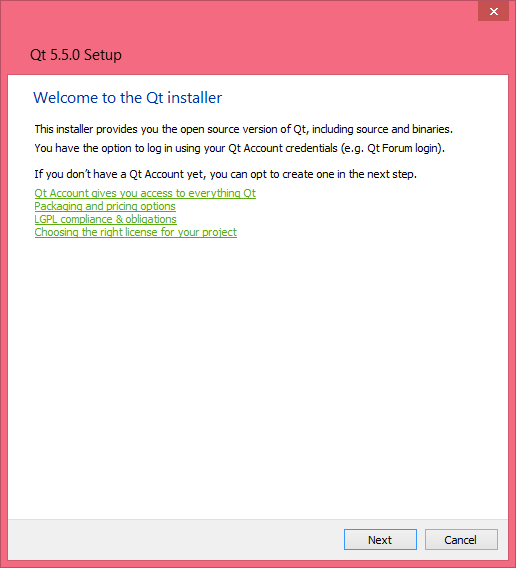
\includegraphics[width=0.4\textwidth]{install-qt-1}
\end{center}
 



\paragraph{Langkah 2}
  Pilih \textbf{Next} dan akan muncul halaman Qt Acount jika anda tidak
  ingin mendatarkan diri dapat di lewati dengan memilih \textbf{skip}.

\begin{center}
	 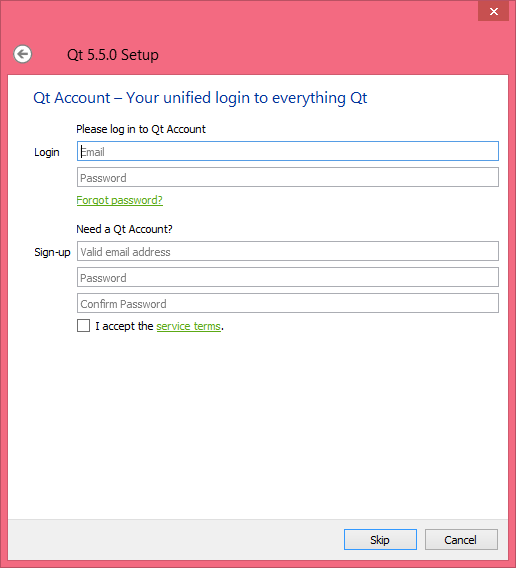
\includegraphics[width=0.4\textwidth]{install-qt-2}
\end{center}
 


  
\paragraph{Langkah 3}
  Masuk ke halaman Setup terus \textbf{next} saja.

  
\begin{center}
	 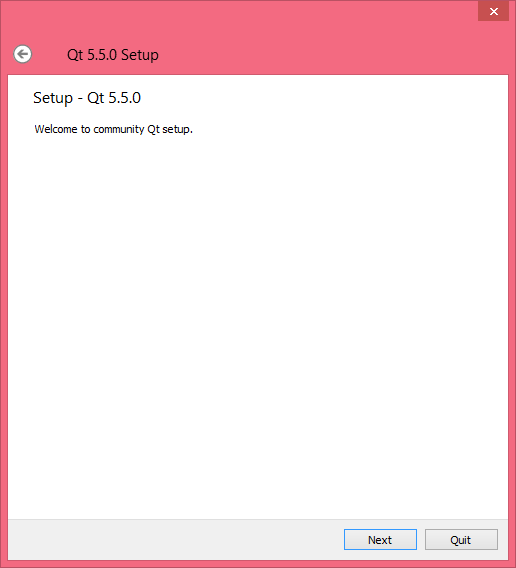
\includegraphics[width=0.4\textwidth]{install-qt-3}
\end{center}
 


  
\paragraph{Langkah 4}
  Installer akan menginstall aplikasi sampai selesai apabila telah
  selesai maka klik finish untuk mengakhiri proses pemasangan aplikasi.


  


\begin{center}

	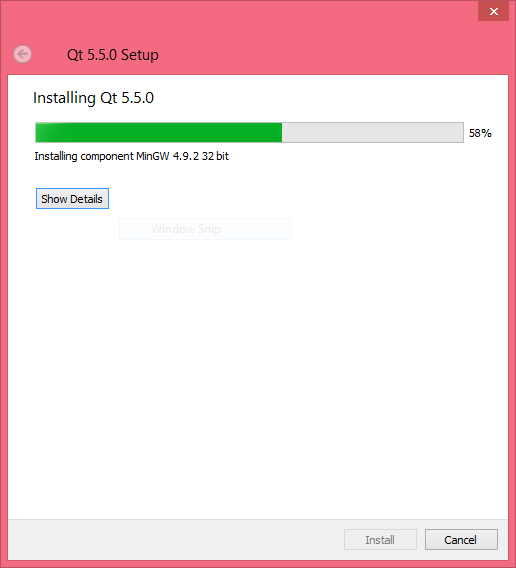
\includegraphics[width=0.4\textwidth]{install-qt-4}
\end{center}

\section{Program Console Pertama dengan Qt
Creator}\label{program-console-pertama-dengan-qt-creator}



  Untuk mencoba membuat aplikasi dengan Qt Creator maka kita perlu
  dengan membuat menu file \textgreater{} new Project dan pilih project
  aplication \textgreater{} Qt console aplication

  \begin{center}

  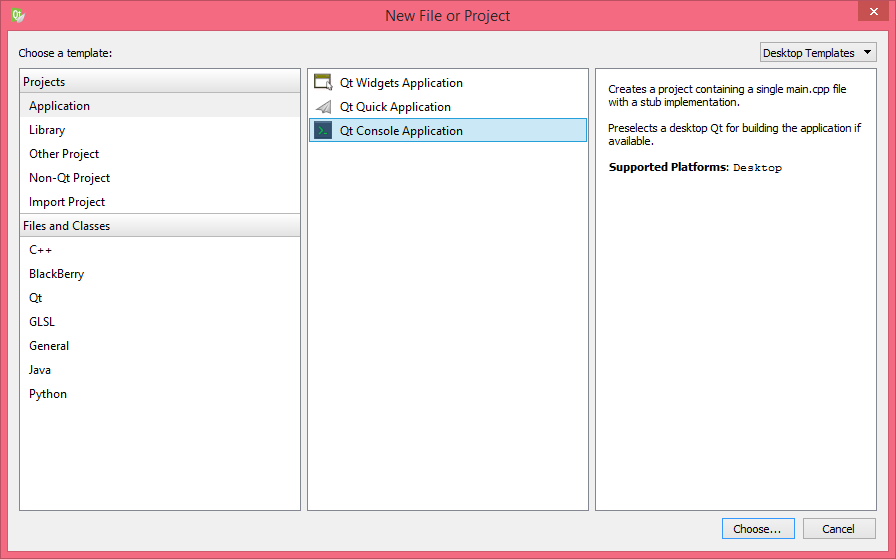
\includegraphics[width=0.8\textwidth]{qt-console-aplication}

  \end{center}

  kemudian beri nama dengan Program yang akan kita buat dan direktori
  tempat aplikasi yang kita buat.

  \begin{center}

  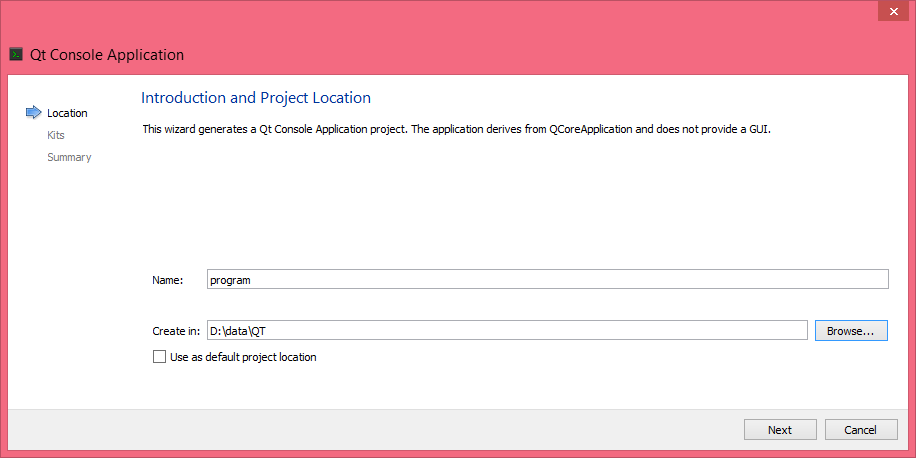
\includegraphics[width=0.8\textwidth]{qt-console-aplication-2}

  \end{center}

  Klik Next, kemudian pilih compiler yang akan kita gunakan. Disini
  penulis menggunakan MinGW sebagai compilernya.


\begin{quotation}
{\LARGE \ding{46}}	\textbf{Tips}
	
	Simulator 	 atau compiler yang lengkap teridir dari
	
	\begin{dinglist}{51}
		
		\item
		Qt Simulator MingGW 4.4
		\item
		Qt Simulator VS 2008, 2010, 2011, 2012 2013, 2014
		\item
		Android SDK dan NDK
	\end{dinglist}
\end{quotation}




\begin{center}

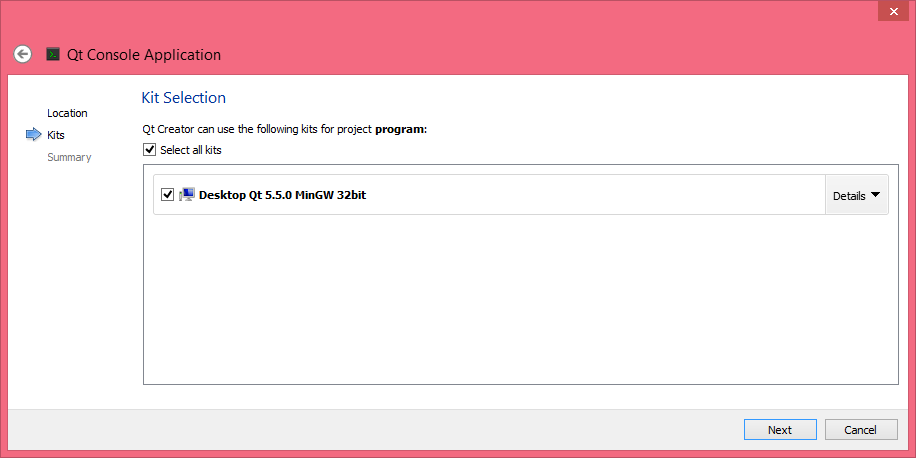
\includegraphics[width=0.8\textwidth]{qt-console-aplication-3}

\end{center}

\begin{enumerate}

\setcounter{enumi}{3}

\item
  Kemudian pilih jenis sub version yang akan kita gunakan, jika Anda
  tidak mengunakan sub version maka pilih none pada add to subversion.
\end{enumerate}

\begin{figure}[htbp]
\centering
\shadowimage[width=8cm]{qt-console-aplication-4}
\caption{Langkah 1 Setup Qt Creator }
\end{figure}

\begin{enumerate}

\setcounter{enumi}{4}

\item
  Apabila di lakukan dengan benar maka akan muncul Qt Editor sebagai
  berikut ini.
\end{enumerate}

\begin{center}

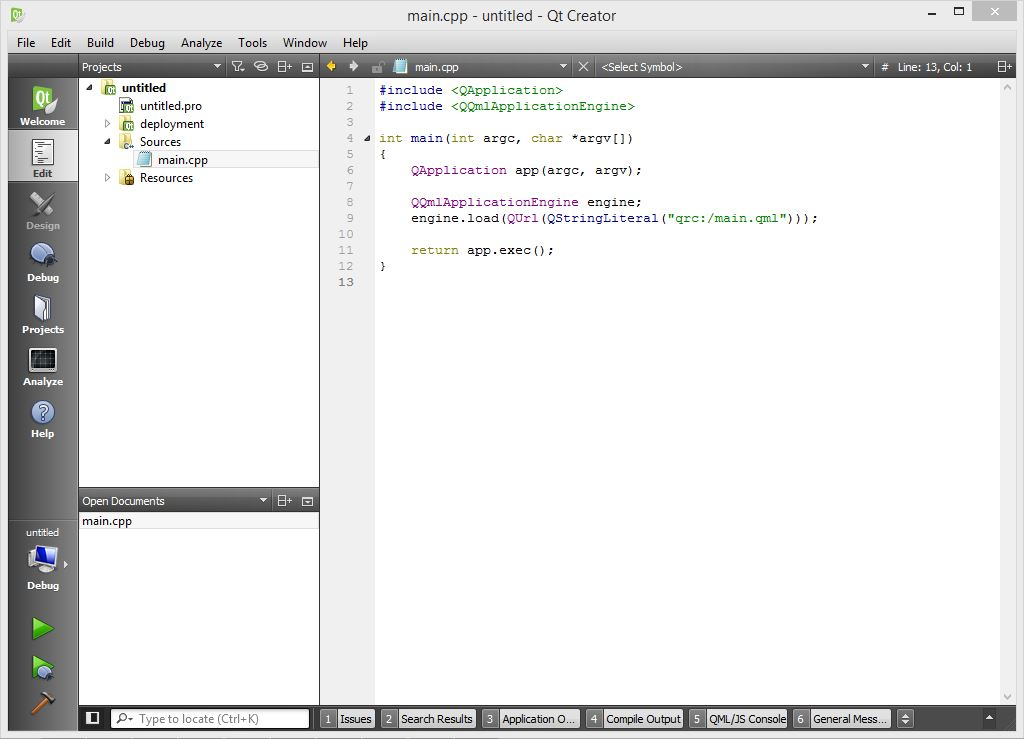
\includegraphics[width=0.8\textwidth]{qt-creator}

\end{center}

\section{Struktur Program C++}\label{struktur-program-cpp}

Program Bahasa C/C++ tidak mengenal aturan penulisan di kolom/baris
tertentu, jadi bisa dimulai dari kolom/baris manapun. Namun demikian,
untuk mempermudah pembacaan program dan untukkeperluan dokumentasi,
sebaiknya penulisan program di bahasa C/C++ diatur sedemikian rupa
sehingga mudah dan enak dibaca. Berikut adalah struktur dasar program
yang dibuat dengan bahasa C++.

\begin{lstlisting}[language=c++, caption=Struktur Program C++]
#include <header>  
using namespace std;    
int main(int argc, char *argv[])
{  
deklarasi variabel;   
deklarasi konstanta;  
perintah perintah;  
//komentar  
return 0;  
}  
\end{lstlisting}

\subsection*{Penjelasan :}

\subsubsection*{ 1. \#include <header>}

\texttt{\#include} adalah salah satu pengarah preprocessor directive
yang tersedia pada C++. Preprocessor selalu dijalankan terlebih dahulu
pada saat proses kompilasi terjadi. Bentuk umumnya:

\begin{lstlisting}[language=c++, numbers=none]
# include <nama_file>
\end{lstlisting}

Bagian tersebut tidak diakhiri dengan tanda semicolon, karena bentuk
tersebut bukanlah suatu bentuk pernyataan, tetapi merupakan preprocessor
directive. Baris tersebut menginstruksikan kepada kompiler untuk
menyisipkan file lain dalam hal ini file yang berakhiran .h (file
header) yaitu file yang berisi C++ standard library. Pada C++ ekstensi
.h tidak dituliskan.

Beberap contoh pengikutsertaan berkas adalah.

\begin{dinglist}{241}

\item
  \texttt{\#include\ \textless{}iostream\textgreater{}} : diperlukan
  pada program yang melibatkan objek \texttt{cout} dan \texttt{cin}
\item
  \texttt{\#include\ \textless{}conio\textgreater{}}: diperlukan bila
  melibatkan \texttt{clrscr()}, yaitu perintah untuk membersihkan layar
  dan fungsi \texttt{getch()} untuk menerima sembarang input keyboard
  dari user.
\item
  \texttt{\#include\ \textless{}iomanip\textgreater{}} : diperlukan bila
  melibatkan \texttt{setw()} yang bermanfaat untuk mengatur lebar dari
  suatu tampilan data.
\item
  \texttt{\#include\ \textless{}math\textgreater{}} : diperlukan pada
  program yang menggunakan operasi \texttt{sqrt()} yang bermanfaat untuk
  operasi matematika kuadrat.
\end{dinglist}

\subsubsection*{2. using namespace std;}\label{using-namespace-std}

Semua elemen standard C++ library dinyatakan dalam apa yang disebut
namespace, namespace tersebut bernama std. Jadi artinya untuk mengakses
semua fungsionalitas std kita menuliskan bahwa kita menggunakan
namespace std.

\subsubsection*{3. int main ()}\label{int-main}

Program C++ terdiri dari satu atau lebih fungsi, dan di antara salah
satunya harus ada fungsi main dan hanya boleh ada satu main pada tiap
program C++. Setiap program C++ akan dan pasti akan memulai eksekusi
programnya pada fungsi main ini, meskipun main bukan fungsi yang pertama
ditulis di program. Melihat bentuk seperti itu dapat kita ambil
kesimpulan bahwa batang tubuh program utama berada didalam fungsi
main(). Berarti dalam setiap pembuatan program utama, maka dapat
dipastikan seorangpemrogram menggunakan minimal sebuah fungsi.

Tanda \{ dan pada akhir program terdapat tanda \}. Tanda \{ harus ada
pada setiap awal dari sebuah fungsi dan tentu saja harus diakhiri dengan
tanda \}. Tanda ini digunakan untuk menunjukkan cakupan(scope) dari
sebuah fungsi,dimana untukmenunjukkan fungsi ini dimulai danberakhir.

\subsubsection*{4. Komentar}\label{komentar}

Komentar tidak pernah dicompile oleh compiler. Dalam C++ terdapat 2
jenis komentar, yaitu:

\begin{lstlisting}[language=c++, numbers=none]

  /* Komentar anda diletakkan
   di dalam ini bisa mengapit
    lebih dari satu  baris */

  // Komentar anda diletakkan disini
  // ( hanya bisa sebaris )
\end{lstlisting}

Programmer sering sekali memasukkan komentar di dalam code agar program
lebih mudah dibaca. Komentar juga membantu orang lain untuk membaca dan
mengerti isi dari code. Komentar tidak menyebabkan komputer melakukan
suatu instruksi ketika program dijalankan.

\subsubsection*{5. Tanda Semicolon (;)}\label{tanda-semicolon}

Tanda semicolon `` \texttt{;} '' digunakan untuk mengakhiri sebuah
pernyataan. Setiap pernyataan harus diakhiri dengan sebuah tanda
semicolon.

\subsubsection*{9. return 0}\label{return-0}

Pernyataan return menyebabkan fungsi utama untuk menyelesaikan
kegiatannya lalu mengembalikanhasil dari fungsi utama. Kode kembalian
biasanya angka 0 atau 1. Jika angka yang dikembalikan 0 berartiprogram
berakhir dengan tidak ada error, sedangkan jika 1 maka program berakhir
dengan error.

\subsubsection{Contoh Structur program C++}

Untuk lebih jelasnya silahkan coba ketik program berikut pada project
baru.

\begin{lstlisting}[language=c++, caption= struktur program C++]
#include <QtCore/QCoreApplication>  
#include <iostream>  
using namespace std;  
int main (int argc, char *argv [])  
{  
QCoreApplication a (argc, argv);  
cout<<"Hello World"<<endl;  
cout<<"Selamat Belajar C/C++ ";  
cout<<"enter my World";  
return a.exec ();  
}
\end{lstlisting}

Kemudian jalankan dengan menekan tombol Run (CTRL + R)

\begin{lcverbatim}
Hello world
Selamat belajar C/C++ enter my world
\end{lcverbatim}


Tampilan Hello World diakhiri dengan tanda enter baru kemudian
dilanjutkan dengan tulisan berikutnya yaitu Selamat Belajar C/C++ enter
my World. Artinya perintah \texttt{endl} merupakan perintah untuk
memberi tanda enter. Sedangkan untuk tulisan Selamat Belajar C/C++ dan
tulisan enter my World yang pada source code terpisah dengan perintah
\texttt{cout}, pada tampilan hasil program tetap sama dan tidak ada
enter diantaranya. Hal ini karena tidak ada perintah untuk menampilkan
enter diantara kedua kalimat tersebut. Penulisan pada kode tidak akan
mempengaruhi hasil output program.

	
	\chapter{Tipe Data, Identifier dan Operator}
	\textbf{Agenda}

Pada bab ini kita akan membahas beberapa topik yang berhubungan dengan tipe data dan Indentifier yaitu:

\minitoc

\section{Tipe Data dan Identifier}\label{tipe-data-dan-identifier}

\index{Program}Program adalah kumpulan instruksi yang disusun sedemikian rupa sehingga
mempunyai urutan nalar yang tepat untuk menyelesaikan suatu persoalan.
Instruksi-instruksi yang digunakan dalam pemrograman mengacu pada suatu
bahasa pemrograman tertentu, pada buku ini menggunakan bahasa
pemrograman C++, sehingga penulisan program pada buku ini mengikuti tata
bahasa C++.

Segala sesuatu yang diproses oleh program adalah data. Dalam hal ini
data adalah elemen-elemen yang digunakan untuk menjelaskan segala
sesuatu yang mempunyai besaran (ukuran/ nilai), seperti misalnya
\textbf{umur} besarannya bisa berupa biangan desimal \textbf{42.5}
(maksudnya 42\textonehalf{} tahun), \textbf{golongan} seorang karyawan besarannya
bisa berupa sebuah karakter A (maksudnya goongan A) dan sebagainya.
Bahasa C++ menyimpan besaran-besaran tersebut di memori utama untuk
dikelola oleh program, sehingga perlu dilakukan pengaturan pemakaian
memori, oleh karena itu dalam bahasa pemrograman selalu terdapat
istilah-istilah yang bernama \textbf{Tipe Data}, \textbf{Variabel} dan
\textbf{Konstanta}\index{konstanta}.

Identifier (pengenal) adalah suatu nama yang digunakan program untuk
merujuk ke suatu lokasi memori tertentu agar nilai pada lokasi tersebut
dapat diakses. Alamat lokasi memori sebenarnya berupa angka angka
heksadesimal\index{heksadesimal}, namun pada bahasa pemrograman
setingkat C++ (middle level programming language)
\index{middle level programming language} dan di atasnya, telah
mengubahnya dalam bentuk identifier (pengenal) yaitu berupa suatu huruf
atau kata (label) sehingga kita tidak perlu mengetahu alamat yang
sesungguhnya dan dengan identifier\index{identifier} (label) akan lebih mudah untuk
diingat.

\section{Tipe Data Bahasa C++}\label{tipe-data-bahasa-c}

Data yang dapat dikelola oleh program bisa bermacam-macam, seperti
misalnya bilangan bulat (\emph{integer}), bilangan dengan desimal
(\emph{floating point}), huruf (\emph{character}), dan sebagainya. Oleh
sebab itu ketika kita akan memakai suatu lokasi memori tertentu untuk
menyimpan nilai diperlukan 2 hal, yaitu \texttt{identifier} sebagai
pengenal (label) lokasi memori yang digunakan dan \texttt{tipe\ data},
yaitu besaran yang menentukan ukuran memori yang dialokasikan. Sekali
suatu identifier sudah dialokasikan dengan tipe data tertentu besarnya
ruang yang digunakan tidak bisa diubah. Bahasa C++ mengenal tipe-tipe
tabel berikut ini.


\begin{longtable}[]{@{}lll@{}}
\toprule
Tipe Data & Ukuran & Jangkauan Nilai Yang dapat Ditampung\tabularnewline
\midrule
\endhead
bool & 1 byte & True or false\tabularnewline
unsigned short int & 2 bytes & 0 to 65,535\tabularnewline
short int & 2 bytes & --32,768 to 32,767\tabularnewline
unsigned long int & 4 bytes & 0 to 4,294,967,295\tabularnewline
long int & 4 bytes & --2,147,483,648 to 2,147,483,647\tabularnewline
int (16 bit) & 2 bytes & --32,768 to 32,767\tabularnewline
int (32 bit) & 4 bytes & --2,147,483,648 to 2,147,483,647\tabularnewline
unsigned int (16 bit) & 2 bytes & 0 to 65,535\tabularnewline
unsigned int (32 bit) & 4 bytes & 0 to 4,294,967,295\tabularnewline
char & 1 byte & 256 character values\tabularnewline
float & 4 bytes & 1.2e--38 to 3.4e38\tabularnewline
double & 8 bytes & 2.2e--308 to 1.8e308\tabularnewline
\bottomrule

\end{longtable}


\section{Variabel dan Konstanta}\label{variabel-dan-konstanta}

Nilai yang tersimpan di memori dan dikenal melalui identifier tersebut
terdiri dari variabel dan konstanta. Perbedaan diantara keduanya adalah
bahwa variabel (sesuai dengan namanya) nilainya dapat diubah-ubah pada
saat program dieksekusi, sedangkan konstanta nilainya tidak dapat diubah
(\texttt{konstan\ =\ tetap}).

Sebelum suatu variabel atau konstanta dapat digunakan, tempat pada
memori harus dipesan terlebih dahulu, mekanisme ini dinamalan deklarasi.
Deklarasi dilakukan dengan cara menuliskan tipe data (ukuran memori yang
dibutuhkan) dan diikuti dengan nama pengenal (nama variabel), jika
dikehendaki bisa juga suatu variabel langsung diinisialisasi dengan
suatu nilai. Pengenal (identifier) bisa terdiri dari sebuah huruf atau
kombinasi antara huruf dengan angka dengan syarat.

\begin{itemize}

\item
  Harus diawali dengan huruf
\item
  Tidak boleh memakai karakter khusus kecuali \$ dan garis bawah (\_)
\item
  Tidak boleh sama dengan kata kunci yang digunakan pada C++
\item
  Bersifat case sensitif (huruf besar dan kecil dibedakan)
\end{itemize}

Walaupun demikian, sebaiknya memberikan nama pengenal variabel sesuai
dengan isi dari variabel tersebut, sebab walaupun nama variabel
``\textbf{c21i8k}'' untuk menyimpan nama mahasiswa adalah valid
(diperbolehkan), namun akan lebih mudah dimengerti jika identifier yang
dipilih adalah ``\textbf{nama}''.

Konstanta mirip dengan variabel, hanya saja nilainya konstan, tidak
dapat diubah-ubah. Untuk dapat membuat konstanta diperlukan inisialisasi
ketika konstanta dibuat dan setelah itu nilainya tidak dapat diubah. C++
mempunyai 2 macam konstanta, yaitu konstanta literal dan konstanta
simbolik. Berikut ini adalah contoh deklarasi variabel:

\begin{lstlisting}[language=c++, numbers=none]
int harga;
\end{lstlisting}

Yang dimaksud dengan konstanta literal adalah suatu nilai yang ditulis
pada kode program. Sebagai contoh misalnya :

\begin{lstlisting}[language=c++, numbers=none]
int usiaku = 42;
\end{lstlisting}

Nilai 42 tidak dapat menerima nilai lain dan nilai tersebut bersifat
tetap. Perhatikan dalam hal ini identifier ``usiaku'' adalah variabel
(bukan konstanta), yang dinamakan konstanta literal adalah nilai ``42''
tersebut.

Konstanta simbolik adalah konstanta yang direpresentasikan dengan suatu
nama, sama seperti variabel, namun berbeda dengan variabel setelah suatu
konstanta diinisialisasi dengan suatu nilai maka nilainya tidak dapat
diubah. Ada 2 cara untuk mendeklarasikan konstanta simbolik, yaitu
dengan menggunakan preprocessor directive \texttt{\#define} dan yang
kedua adalah dengan memakai kata kunci \texttt{const}. Berikut ini
contoh mendeklarasikan dan menginisialisasi konstanta :

\begin{lstlisting}[language=c++, numbers=none]
#define kapasitas 15
\end{lstlisting}

Perhatikan bahwa \texttt{kapasitas} tidak mempunyai tipe data tertentu
(int, char dsb.). Preprosessor akan melakukan substitusi berupa teks,
setiap ada akses terhadap kata \texttt{kapasitas}, akan digantikan
dengan teks 15. Karena preprosesor bekerja sebelum kompiler, kompiler
tidak mengenal konstanta \texttt{kapasitas}, yang dikenal hanyalah
bilangan 15.

\begin{quotation}

\includegraphics{../manuscript/images/tips}\textbf{TIPS} 

Walaupun
dengan memakai preprocessor directive \texttt{\#define} tampak mudah,
namun sebaiknya cara ini tidak digunakan, karena sudah dinyatakan usang
pada standard C++ .
\end{quotation}
 

Cara yang kedua untuk menginisialisasi sebuah konstanta adalah dengan
memakai kata kunci const seperti berikut :

\begin{lstlisting}[language=c++, numbers=none]
const int usiaku = 42;
\end{lstlisting}

Contoh diatas adalah mendeklarasikan konstanta simbolik bernama usiaku
bertipe int dan diinisialisasi dengan nilai 42. Setelah baris ini simbol
(identifier) bernama usiaku tidak dapat diubah-ubah nilainya. Keuntungan
pembuatan konstanta dengan cara ini adalah lebih mudah dipelihara dan
mencegah adanya kesalahan dan yang paling penting adalah bahwa konstanta
ini mempunyai tipe data dan kompiler dapat mengharuskan konstanta ini
diperlakukan sebagai tipe data tersebut.

\subsubsection*{Contoh Tipe data dan Identifier.}

\begin{enumerate}

\item
  Buka Qt Creator dan buat project Qt Console Application baru dengan
  nama contoh \ref{contoh2-1}, kemudian tulis kode berikut.

\lstinputlisting[language=c++, caption=Tipe data dan Identifier, label=contoh2-1]{../code/contoh2-1.cpp}

\item
  Kemudian jalankan kode diatas dengan menekan tombol Ctrl+R, outputnya
  adalah sebagai berikut.

\begin{lcverbatim}
Panjang =15
lebar =12
\end{lcverbatim}

\end{enumerate}


\subsubsection*{Keterangan}

\begin{itemize}

\item
  Pada program di atas variabel panjang dan lebar dideklarasikan bertipe
  int.
\item
  Kemudian variabel panjang diberi nilai 15 (integer) dan lebar diberi
  nilai 12 (integer), tampak bahwa nilai dari variabel tersebut dapat
  diubah.
\item
  Pada baris berikutnya nilai dari variabel dapat diakses untuk dicetak
  ke layar.
\end{itemize}

\section{Statement}\label{statement}

Dalam bahasa C++, sebuah statement mengontrol urutan pengerjaan
eksekusi, mengevaluasi ekspresi atau tidak mengejakan apapun (\emph{null
statement}). Semua statement C++ diakhiri dengan titik koma (;), sebagai
contoh misalnya :

\begin{lstlisting}[language=c++, numbers=none]
x = a + b;
\end{lstlisting}

Pernyataan tersebut bukanlah suatu pernyataan persamaan aljabar dalam
matematika yang artinya x sama dengan a + b, melainkan memberi nilai x
dengan hasil penjumlahan a dengan b. Pada statement ini terjadi 2 urutan
pengerjaan, yaitu pertama menambahkan a dengan b, kemudian yang kedua
memberikan hasil perhitungan tersebut ke variabel x dengan operator
pengerjaan (=). Walaupun pada pernyataan tersebut terdapat 2 pekerjaan,
namun merupakan sebuah statement dan oleh karena itu diakhiri hanya
dengan sebuah titik koma (;) saja. Hasil penjumlahan a dengan b ini
disebut ekspresi, sedangkan sama dengan (=) dan plus (+) dinamakan
operator yang akan dibahas berikut ini.

\begin{quotation}

\includegraphics{../manuscript/images/pencil} \textbf{CATATAN}
 
 Operator pengerjaan = akan mengambil nilai apapun yang ada disebelah
 kanannya kenudian memberikannya kepada apapun yang berada di sebelah
 kirinya. C++ mengenal juga operator pembanding == yang mempunyai
 arti berbeda dengan operator sama dengan =, akan dibahas lebih
 detail pada sub bab berikut ini.
\end{quotation}


\section{Operator dan Ekspresi}\label{operator-dan-ekspresi}

Operator adalah suatu simbol yang digunakan untuk melakukan suatu
operasi. Operator mempunyai beberapa kategori, antara lain : Aritmatika,
Pengerjaan, Hubungan dan Logika. Operator Aritmatika adalah operator
yang digunakan untuk melakukan operasi aritmatika seperti misalnya
penjumlahan, pengurangan, perkalian dan pembagian. Simbol untuk operator
aritmatika ini adalah : +, -, *, / dan \%. Berikut ini adalah
operator-operator yang dikenal pada bahasa pemrograman C++.

\begin{longtable}[]{@{}llll@{}}
\toprule
\begin{minipage}[b]{0.52\columnwidth}\raggedright\strut
Kategori
\strut\end{minipage} &
\begin{minipage}[b]{0.17\columnwidth}\raggedright\strut
Operator
\strut\end{minipage} &
\begin{minipage}[b]{0.14\columnwidth}\raggedright\strut
Arah Proses
\strut\end{minipage} &
\begin{minipage}[b]{0.05\columnwidth}\raggedright\strut
Jenjang
\strut\end{minipage}\tabularnewline
\midrule
\endhead
\begin{minipage}[t]{0.52\columnwidth}\raggedright\strut
Kurung, indeks larik dan elemen struktur data
\strut\end{minipage} &
\begin{minipage}[t]{0.17\columnwidth}\raggedright\strut
() {[}{]} . -\textgreater{}
\strut\end{minipage} &
\begin{minipage}[t]{0.14\columnwidth}\raggedright\strut
Kiri - Kanan
\strut\end{minipage} &
\begin{minipage}[t]{0.05\columnwidth}\raggedright\strut
1
\strut\end{minipage}\tabularnewline
\begin{minipage}[t]{0.52\columnwidth}\raggedright\strut
Operator Unary
\strut\end{minipage} &
\begin{minipage}[t]{0.17\columnwidth}\raggedright\strut
! \textasciitilde{} - ++ --
\strut\end{minipage} &
\begin{minipage}[t]{0.14\columnwidth}\raggedright\strut
Kanan -- Kiri
\strut\end{minipage} &
\begin{minipage}[t]{0.05\columnwidth}\raggedright\strut
2
\strut\end{minipage}\tabularnewline
\begin{minipage}[t]{0.52\columnwidth}\raggedright\strut
Operator Aritmatika Perkalian, Pembagian dan Sisa Pembagian
\strut\end{minipage} &
\begin{minipage}[t]{0.17\columnwidth}\raggedright\strut
* / \%
\strut\end{minipage} &
\begin{minipage}[t]{0.14\columnwidth}\raggedright\strut
Kiri -- Kanan
\strut\end{minipage} &
\begin{minipage}[t]{0.05\columnwidth}\raggedright\strut
3
\strut\end{minipage}\tabularnewline
\begin{minipage}[t]{0.52\columnwidth}\raggedright\strut
Operator aritmatika Pertambahan dan Pengurangan
\strut\end{minipage} &
\begin{minipage}[t]{0.17\columnwidth}\raggedright\strut
+ -
\strut\end{minipage} &
\begin{minipage}[t]{0.14\columnwidth}\raggedright\strut
Kiri -- Kanan
\strut\end{minipage} &
\begin{minipage}[t]{0.05\columnwidth}\raggedright\strut
4
\strut\end{minipage}\tabularnewline
\begin{minipage}[t]{0.52\columnwidth}\raggedright\strut
Operator Bitwise Pergeseran Bit
\strut\end{minipage} &
\begin{minipage}[t]{0.17\columnwidth}\raggedright\strut
\textless{}\textless{} \textgreater{}\textgreater{}
\strut\end{minipage} &
\begin{minipage}[t]{0.14\columnwidth}\raggedright\strut
Kiri -- Kanan
\strut\end{minipage} &
\begin{minipage}[t]{0.05\columnwidth}\raggedright\strut
5
\strut\end{minipage}\tabularnewline
\begin{minipage}[t]{0.52\columnwidth}\raggedright\strut
Operator Hubungan
\strut\end{minipage} &
\begin{minipage}[t]{0.17\columnwidth}\raggedright\strut
\textless{} \textless{}= \textgreater{} \textgreater{}=
\strut\end{minipage} &
\begin{minipage}[t]{0.14\columnwidth}\raggedright\strut
Kiri -- Kanan
\strut\end{minipage} &
\begin{minipage}[t]{0.05\columnwidth}\raggedright\strut
6
\strut\end{minipage}\tabularnewline
\begin{minipage}[t]{0.52\columnwidth}\raggedright\strut
Operator Hubungan Kesamaan dan Ketidaksamaan
\strut\end{minipage} &
\begin{minipage}[t]{0.17\columnwidth}\raggedright\strut
== !=
\strut\end{minipage} &
\begin{minipage}[t]{0.14\columnwidth}\raggedright\strut
Kiri -- Kanan
\strut\end{minipage} &
\begin{minipage}[t]{0.05\columnwidth}\raggedright\strut
7
\strut\end{minipage}\tabularnewline
\begin{minipage}[t]{0.52\columnwidth}\raggedright\strut
Operator Bitwise AND
\strut\end{minipage} &
\begin{minipage}[t]{0.17\columnwidth}\raggedright\strut
\&
\strut\end{minipage} &
\begin{minipage}[t]{0.14\columnwidth}\raggedright\strut
Kiri -- Kanan
\strut\end{minipage} &
\begin{minipage}[t]{0.05\columnwidth}\raggedright\strut
8
\strut\end{minipage}\tabularnewline
\begin{minipage}[t]{0.52\columnwidth}\raggedright\strut
Operator Bitwise XOR
\strut\end{minipage} &
\begin{minipage}[t]{0.17\columnwidth}\raggedright\strut
\^{}
\strut\end{minipage} &
\begin{minipage}[t]{0.14\columnwidth}\raggedright\strut
Kiri -- Kanan
\strut\end{minipage} &
\begin{minipage}[t]{0.05\columnwidth}\raggedright\strut
9
\strut\end{minipage}\tabularnewline
\begin{minipage}[t]{0.52\columnwidth}\raggedright\strut
Operator Bitwise OR
\strut\end{minipage} &
\begin{minipage}[t]{0.17\columnwidth}\raggedright\strut
\texttt{\textbar{}}
\strut\end{minipage} &
\begin{minipage}[t]{0.14\columnwidth}\raggedright\strut
Kiri -- Kanan
\strut\end{minipage} &
\begin{minipage}[t]{0.05\columnwidth}\raggedright\strut
10
\strut\end{minipage}\tabularnewline
\begin{minipage}[t]{0.52\columnwidth}\raggedright\strut
Operator Kondisi AND
\strut\end{minipage} &
\begin{minipage}[t]{0.17\columnwidth}\raggedright\strut
\&\&
\strut\end{minipage} &
\begin{minipage}[t]{0.14\columnwidth}\raggedright\strut
Kiri -- Kanan
\strut\end{minipage} &
\begin{minipage}[t]{0.05\columnwidth}\raggedright\strut
11
\strut\end{minipage}\tabularnewline
\begin{minipage}[t]{0.52\columnwidth}\raggedright\strut
Operator Kondisi OR
\strut\end{minipage} &
\begin{minipage}[t]{0.17\columnwidth}\raggedright\strut
\texttt{\textbar{}\textbar{}}
\strut\end{minipage} &
\begin{minipage}[t]{0.14\columnwidth}\raggedright\strut
Kiri -- Kanan
\strut\end{minipage} &
\begin{minipage}[t]{0.05\columnwidth}\raggedright\strut
12
\strut\end{minipage}\tabularnewline
\begin{minipage}[t]{0.52\columnwidth}\raggedright\strut
Operator Ternary ?
\strut\end{minipage} &
\begin{minipage}[t]{0.17\columnwidth}\raggedright\strut
\texttt{\textbar{}}
\strut\end{minipage} &
\begin{minipage}[t]{0.14\columnwidth}\raggedright\strut
Kanan -- Kiri
\strut\end{minipage} &
\begin{minipage}[t]{0.05\columnwidth}\raggedright\strut
13
\strut\end{minipage}\tabularnewline
\begin{minipage}[t]{0.52\columnwidth}\raggedright\strut
Operator Pengerjaan Aritmatika
\strut\end{minipage} &
\begin{minipage}[t]{0.17\columnwidth}\raggedright\strut
= += -= *= /= \%=
\strut\end{minipage} &
\begin{minipage}[t]{0.14\columnwidth}\raggedright\strut
Kanan -- Kiri
\strut\end{minipage} &
\begin{minipage}[t]{0.05\columnwidth}\raggedright\strut
14
\strut\end{minipage}\tabularnewline
\begin{minipage}[t]{0.52\columnwidth}\raggedright\strut
Operator Pengerjaan Bitwise
\strut\end{minipage} &
\begin{minipage}[t]{0.17\columnwidth}\raggedright\strut
\texttt{\&=\ \^{}=\ \textbar{}=\ \textless{}\textless{}=\ \textgreater{}\textgreater{}=}
\strut\end{minipage} &
\begin{minipage}[t]{0.14\columnwidth}\raggedright\strut
Kanan -- Kiri
\strut\end{minipage} &
\begin{minipage}[t]{0.05\columnwidth}\raggedright\strut
15
\strut\end{minipage}\tabularnewline
\begin{minipage}[t]{0.52\columnwidth}\raggedright\strut
Operator Koma
\strut\end{minipage} &
\begin{minipage}[t]{0.17\columnwidth}\raggedright\strut
,
\strut\end{minipage} &
\begin{minipage}[t]{0.14\columnwidth}\raggedright\strut
Kiri -- Kanan
\strut\end{minipage} &
\begin{minipage}[t]{0.05\columnwidth}\raggedright\strut
16
\strut\end{minipage}\tabularnewline
\bottomrule
\end{longtable}

Ekspresi adalah suatu peryataan yang menghasilkan suatu nilai, bisa
berasal dari sebuah variabel maupun kumpulan variabel-variabel yang
dioperasikan dengan suatu operator, jadi hasil akhir dari suatu ekspresi
adalah suatu nilai yang mempunyai besaran dan tipe data tertentu.

Pernyataan berikut ini yang disebut ekspresi adalah 15, 12 dan ``panjang
* lebar'' yang menghasilkan nilai 15, 12 dan 180:

\begin{lstlisting}[language=c++, numbers=none]
panjang = 15;
lebar = 12;
luas = panjang * lebar ;
\end{lstlisting}

\textbf{Keterangan :}

\begin{itemize}

\item
  Pada baris pertama dan kedua di atas digunakan hanya sebuah operator
  \texttt{=} (yaitu jenjang ke 14), arah proses dari kanan ke kiri,
  sehingga yang dilakukan :
\item
  Ekspresi : \texttt{15}, diberikan kepada variabel \texttt{panjang}
  (dibaca dari kanan ke kiri).
\item
  Ekspresi : \texttt{12}, diberikan kepada variabel \texttt{lebar}
  (dibaca dari kanan ke kiri).
\item
  Pada baris ketiga terdapat 2 operator, yaitu operator =  (jenjang
  ke 14) dan \texttt{*} operator = (yaitu jenjang ke 3).
  Jenjang menunjukkan operator yang akan dikerjakan terlebih dahulu,
  jika dalam sebuah ungkapan terdapat lebih dari satu jenis operator.
  Jenjang nomor 1 adalah jenjang yang paling tinggi, maka pada
  pernyataan di atas yang akan dikerjakan terlebih dahulu adalah orator
  \texttt{*} baru kemudian operator =, sehingga yang dilakukan:
  - Ekspresi : \texttt{panjang\ *\ lebar} , berarti \texttt{panjang}
  dikalikan \texttt{lebar} (dibaca dari kiri ke kanan), menghasilkan
  nilai integer \texttt{180}. - Berikutnya operator = mengoperasikan
  hasil ekspresi tersebut, yaitu nilai integer \texttt{180} diberikan
  kepada variabel \texttt{luas} (dibaca dari kanan ke kiri).
\end{itemize}

\begin{quotation}

\includegraphics{../manuscript/images/tips}\textbf{TIPS}

Operator
( dan ) dapat dipakai untuk merubah jenjang suatu ekspresi
menjadi jenjang tertinggi, sehingga akan diproses terlebih dahulu.
\end{quotation}


\subsection{ Operator Unary}\label{a-operator-unary}

Operator unary adalah operator yang hanya menggunakan sebuah operand
saja, operator unary yang dipakai pada kebanyakan bahasa pemrograman
adalah operator unary minus (-). Operator unary ditulis sebelum operand,
operator unary ``-'' berbeda dengan operator aritmatika ``-'' yang
membutuhkan dua operand. Dalam bahasa C++ disediakan bermacam-macam
operator unary.

\begin{longtable}[]{@{}ll@{}}
\toprule
Operator & Arti\tabularnewline
\midrule
\endhead
- & Unary minus\tabularnewline
++ & Peningkatan dengan nilai penambahan 1\tabularnewline
-- & Penurunan dengan nilai pengurangan 1\tabularnewline
! & Unary not\tabularnewline
\textasciitilde{} & Operator unary komplemen satu (bitwise
NOT)\tabularnewline
\bottomrule
\end{longtable}

\subsection{Operator Unary Minus}\label{b-operator-unary-minus}

Operator ini dipakai untuk memberi nilai minus suatu nilai numerik
(bukan pengurangan). Misalnya ungkapan : \texttt{A\ +\ -\ B\ *\ C} akan
diartikan \texttt{A\ +\ (-B)\ *\ C}. Operator unary ``-'' ditulis di
depan operand.

\subsection{Operator Unary ++ dan --}\label{c-operator-unary-dan}

Operator unary ``++'' dan ``--'' merupakan operator khusus yang ada di
bahasa C. Operator ``++'' akan menambahkan nilai 1 ke pengenal yang
menggunakannya sedangkan operator ``--'' akan mengurangi dengan nilai
numerik 1. Operator unary tersebut jika dituliskan sebelum operand
disebut \emph{pre increment} sedangkan jika ditulis setelah operand
disebut \emph{post increment}. Perhatikan perbedaannya pada contoh
dibawah ini :

\begin{longtable}[]{@{}ll@{}}
\toprule
Post Increment & Pre Increment\tabularnewline
\midrule
\endhead
x = 5; & x = 5;\tabularnewline
a = x++; & a = ++x;\tabularnewline
------------------- & ----------------\tabularnewline
\textbf{Hasil:} & \textbf{Hasil:}\tabularnewline
x = 6 dan a = 5 & x = 6 dan a = 6\tabularnewline
\bottomrule
\end{longtable}

\subsection{Operator Pengerjaan}\label{d-operator-pengerjaan}

Operator pengerjaan atau disebut assignment operator, digunakan untuk
menempatkan nilai dari suatu ekspresi ke suatu pengenal. Operator yang
umum dipakai pada bahasa pemrograman adalah operator pengerjaan ``=''.
Selain operator pengerjaan ``='', bahasa C++ menyediakan beberapa
operator pengerjaan yang lain seperti tabel di bawah ini.

\begin{longtable}[]{@{}lll@{}}
\toprule
Operator & Contoh & Maksud/ Ekuivalen dengan\tabularnewline
\midrule
\endhead
= & a = b + c & Mengerjakan b+c ke a\tabularnewline
+= & a += 1 & a = a + 1\tabularnewline
-= & a -= b & a = a -- b\tabularnewline
*= & a *= b & a = a * b\tabularnewline
/= & a /= b & a = a / b\tabularnewline
\%= & a \%= b & a = a \% b\tabularnewline
\bottomrule
\end{longtable}

Tabel berikut ini memberikan contoh pemakaian operator-operator di atas,
misalnya variabel a dan b bernilai 10.

\begin{longtable}[]{@{}lll@{}}
\toprule
Statement & Ekuivalen dengan & Hasil Ungkapan\tabularnewline
\midrule
\endhead
a += 3 & a = a + 3 & a = 10 + 3 = 13\tabularnewline
a -= 2 & a = a - 2 & a = 10 -- 2 = 8\tabularnewline
a *= b/2 & a = a * (b/2) & a = 10 * (10/2) = 50\tabularnewline
a /= b -- 8 & a = a / (j -- 8) & a = 10 / (10-8) = 5\tabularnewline
\bottomrule
\end{longtable}

Dari contoh di atas terlihat bahwa operator pengerjaan mempunyai jenjang
yang lebih rendah dibanding operator aritmatika, sehingga operator
aritmatika dikerjakan terlebih dahulu.

C++ mengijinkan operator pengerjaan ditulis lebih dari satu kali pada
sebuah statement, misalnya :

\begin{lstlisting}[language=c++, numbers=none]
x = y = a * b;
\end{lstlisting}

Dalam hal ini yang dikerjakan adalah a dikalikan b terlebih dahulu
meudian hasilnya diberikan kepada variabel y dan hasil ekspresi y = a *
b diberikan kepada variabel x. sehingga misalnya a bernilai 8 dan b
bernilai 7, maka baik variabel x maupun y keduanya bernilai 15.

\subsection{Operator Hubungan}\label{e-operator-hubungan}

Operator hubungan (\emph{relational operator}) digunakan untuk
menunjukkan hubungan antara dua buah operand, hasil dari operator ini
adalah True atau False.

\begin{longtable}[]{@{}lll@{}}
\toprule
Operator & Jenjang & Arti\tabularnewline
\midrule
\endhead
\textless{} & 6 & Lebih kecil dari\tabularnewline
\textless{}= & 6 & Lebih kecil atau sama dengan\tabularnewline
\textgreater{} & 6 & Lebih besar dari\tabularnewline
\textgreater{}= & 6 & Lebih besar atau sama dengan\tabularnewline
== & 7 & Sama dengan\tabularnewline
!= & 7 & Tidak sama dengan\tabularnewline
\bottomrule
\end{longtable}

Berikut ini contoh hasil ekspresi jika a bernilai 5, b bernilai 7 dan c
bernilai `a'

\begin{longtable}[]{@{}lll@{}}
\toprule
Ungkapan Hubungan & Hasil & Nilai\tabularnewline
\midrule
\endhead
a == 5 & Benar & 1\tabularnewline
a == b & Salah & 0\tabularnewline
b \textless{} 7 & Salah & 0\tabularnewline
a \textless{}= 7 & Benar & 1\tabularnewline
(a+b) != 35 & Benar & 1\tabularnewline
c != `A' & Benar & 1\tabularnewline
c \textless{}= `z' & Benar & 1\tabularnewline
\bottomrule
\end{longtable}

\subsection{Operator Logika}\label{f-operator-logika}

Jika operator hubungan membandingkan hubungan antara dua buah operand,
maka operator logika (\emph{logical operator}) digunakan untuk
menggabungkan logika hasil dari operator-operator hubungan. Operator
logika menggabungkan \textbf{dua buah} nilai logika. Nilai logika adalah
nilai benar (True) atau salah (False).

\begin{longtable}[]{@{}lll@{}}
\toprule
Operator & Jenjang & Arti\tabularnewline
\midrule
\endhead
\&\& & 11 & Logika DAN (AND)\tabularnewline
\texttt{\textbar{}\textbar{}} & 12 & Logika ATAU (OR)\tabularnewline
\bottomrule
\end{longtable}

Selain dua operator logika ini, operator unary \textquotedblleft ! \textquotedblright (logika NOT) dapat digunakan untuk operasi logika.

\begin{longtable}[]{@{}lllll@{}}
\toprule
x & y & x \&\& y & x \texttt{\textbar{}\textbar{}} y & !x\tabularnewline
\midrule
\endhead
TRUE & TRUE & TRUE & TRUE & FALSE\tabularnewline
TRUE & FALSE & FALSE & TRUE & FALSE\tabularnewline
FALSE & TRUE & FALSE & TRUE & TRUE\tabularnewline
FALSE & FALSE & FALSE & FALSE & TRUE\tabularnewline
\bottomrule
\end{longtable}

Contoh : Misalnya A bernilai 5, B bernilai 7 dan C bernilai \textquotedblleft a \textquotedblright maka ungkapan dibawah ini mempunyai hasil akhir benar (True).

\begin{lstlisting}[language=c++, numbers=none]
A < B || B == 7 && C > 'z'
\end{lstlisting}

Hasil akhir benar (True) dari ekspresi logika tersebut didapat dari
langkah-langkah sebagai berikut:

\begin{enumerate}


\item
  Jenjang operator hubungan lebih tinggi dibandingkan dengan operator
  logika, jadi operator hubungan dikerjakan terlebih dahulu.
\item
  Operator logika ``\&\&'' mempunyai jenjang lebih tinggi dari operator
  ``\textbar{}\textbar{}'', sehingga operator ``\&\&'' dikerjakan
  terlebih dahulu.
\item
  Bagian yang paling akhir dikerjakan adalah operator
  ``\textbar{}\textbar{}'', sehingga hasil akhir logika bernilai logika
  benar atau True.
\end{enumerate}



	
	\chapter{Control Statement}
	\textbf{📋 Apa yang akan dipelajari}

Pada bab ini kita akan mempelajari tentang Control Statement (Struktur Kendali) dalam C++:

\begin{itemize}
\item Percabangan (if, if-else, switch)
\item Perulangan (for, while, do-while)
\item Kata kunci break dan continue
\end{itemize}

\minitoc

\section{🎯 Pengenalan Control Statement}

Program tidak selalu berjalan secara berurutan dari atas ke bawah. Kadang-kadang kita perlu:
\begin{itemize}
\item \textbf{Percabangan} - memilih jalur program berdasarkan kondisi
\item \textbf{Perulangan} - mengulang perintah tertentu
\item \textbf{Kombinasi} - menggabungkan percabangan dan perulangan
\end{itemize}

Control statement adalah konsep fundamental dalam pemrograman yang memungkinkan program untuk membuat keputusan dan mengulang operasi\footnote{Dijkstra, E. W. (1968). "Go To Statement Considered Harmful". Communications of the ACM.}.

Control Statement adalah pengatur aliran program yang memungkinkan kita:
\begin{itemize}
\item Mengulang perintah jika kondisi tertentu terpenuhi
\item Melanjutkan program jika kondisi terpenuhi
\item Memilih dari beberapa alternatif berdasarkan kondisi
\end{itemize}

\section{🔄 Percabangan (Conditional Statements)}\label{percabangan}

Percabangan adalah perintah yang memungkinkan program memilih jalur yang berbeda berdasarkan kondisi tertentu. 

\subsection{Apa itu Percabangan?}

Percabangan memungkinkan program untuk:
\begin{itemize}
\item Menjalankan kode tertentu jika kondisi terpenuhi
\item Menjalankan kode lain jika kondisi tidak terpenuhi
\item Memilih dari beberapa alternatif berdasarkan nilai tertentu
\end{itemize}

\subsection{Jenis-jenis Percabangan dalam C++}

C++ memiliki tiga jenis perintah percabangan:
\begin{itemize}
\item \textbf{if} - menjalankan kode jika kondisi benar
\item \textbf{if-else} - menjalankan kode berbeda berdasarkan kondisi
\item \textbf{switch} - memilih dari beberapa alternatif berdasarkan nilai
\end{itemize}

\subsection{🔀 Percabangan dengan if}\label{percabangan-dengan-if}

Percabangan \textbf{if} adalah yang paling sederhana. Program akan menjalankan kode di dalam blok if jika kondisi bernilai benar (true). Konsep ini pertama kali diperkenalkan dalam bahasa ALGOL 60\footnote{Naur, P. (1960). "Report on the Algorithmic Language ALGOL 60". Communications of the ACM.}.

\subsubsection{Sintaks if}

\lstinputlisting[language=c++, numbers=none]{../code/control-if-syntax.cpp}

\subsubsection{Cara Kerja if}

\begin{itemize}
\item Program mengecek kondisi dalam kurung
\item Jika kondisi \textbf{benar} (true), kode dalam blok dijalankan
\item Jika kondisi \textbf{salah} (false), kode dalam blok dilewati
\item Program melanjutkan ke baris setelah blok if
\end{itemize}

Flowchart untuk statment percabangan if seperti pada gambar berikut


\begin{tikzpicture}[node distance = 2cm, auto]
\node [ling] (init){start};
\node [decision, below of=init] (decide) {\textless{}ekspresi \_bool\textgreater{}};
\node [block, below of=decide, node distance=3cm] (statement) {Statement};
\node [ling, below of=statement] (stop) {stop};

%garis
\path [line] (init) -- (decide);
\path [line] (init) -- (decide);
\path [line] (decide) -- node {Yes}(statement);
%\path [line] (statement) |- node [near start] {No} (decide);
\path[line] (statement) -- (stop);
\end{tikzpicture}


\subsection*{💡 Contoh Percabangan dengan if}

\begin{enumerate}
\item Buka Qt Creator dan buat project Qt Console Application baru dengan nama "contoh"
\item Tulis kode berikut:

\lstinputlisting[language=c++, caption=Contoh percabangan dengan if, label=contoh2-3]{../code/contoh2-3.cpp}

\item Jalankan program dengan menekan Ctrl + R. Outputnya:

\begin{lcverbatim}
Masukan nomor: 15
15 lebih besar dari 10
\end{lcverbatim}

\subsubsection*{Penjelasan Program}
\begin{itemize}
\item Program meminta input angka dari pengguna
\item Jika angka > 10, program menampilkan pesan "lebih besar dari 10"
\item Jika angka ≤ 10, program tidak menampilkan apa-apa
\end{itemize}
\end{enumerate}
\subsection{🔄 Percabangan dengan if-else}\label{percabangan-dengan-if-..-else}

Percabangan \textbf{if-else} memungkinkan program menjalankan kode yang berbeda berdasarkan kondisi.

\subsubsection{Sintaks if-else}

\lstinputlisting[language=c++]{../code/control-if-else-syntax.cpp}

\subsubsection{Cara Kerja if-else}

\begin{itemize}
\item Program mengecek kondisi dalam kurung
\item Jika kondisi \textbf{benar}, kode dalam blok if dijalankan
\item Jika kondisi \textbf{salah}, kode dalam blok else dijalankan
\item Program selalu menjalankan salah satu blok (if atau else)
\end{itemize}

Flowchart untuk statment ini adalah :

\begin{quotation}
{\LARGE \ding{45}} \textbf{💡 CATATAN PENTING}

Di dalam blok \texttt{if()} maupun \texttt{else} bisa diisi dengan perintah \texttt{if()} lagi. Bentuk \texttt{if()} dalam \texttt{if()} ini sering disebut dengan \textbf{nested if} (if bersarang).
\end{quotation}

\begin{tikzpicture}[node distance = 2cm, auto]
\node [ling] (init){start};
\node [decision, below of=init, node distance=2cm] (decide) {\textless{}ekspresi \_bool\textgreater{}};
\node [block, below of=decide, node distance=3cm] (statement) {Statement};
\node [block, right of=decide, node distance=3cm] (statement2) {Statement2};
\node [ling, below of=statement, node distance=2cm] (stop) {stop};

%garis
\path [line] (init) -- (decide);
\path [line] (init) -- (decide);
\path [line] (decide) -- node {Ya}(statement);
%\path [line] (statement) |- node [near start] {No} (decide);
\path[line] (statement) -- (stop);
\path[line] (statement) -| node {tidak}(statement2);
\path[line] (statement2) -- (decide);
\end{tikzpicture}

\subsubsection*{💡 Contoh Program if-else}

\begin{enumerate}
\item Edit contoh \ref{contoh2-3} dengan menambahkan kode berikut:

\lstinputlisting[language=c++, firstline=13, lastline=14, caption=Contoh percabangan if-else, label=contoh2-4]{../code/contoh2-4.cpp}

\item Jalankan program dengan menekan Ctrl + R. Outputnya:

\begin{lcverbatim}
Masukan nomor: 4
4 kurang besar dari 10
\end{lcverbatim}

\subsubsection*{Penjelasan Program}
\begin{itemize}
\item Jika angka > 10, program menampilkan "lebih besar dari 10"
\item Jika angka ≤ 10, program menampilkan "kurang besar dari 10"
\item Program selalu memberikan respons, tidak ada kondisi yang dilewati
\end{itemize}
\end{enumerate}

\subsection{🔄 Percabangan dengan if Bersarang (Nested if)}

If bersarang adalah kondisi if yang berada di dalam blok if atau else lainnya. Ini memungkinkan kita membuat percabangan yang lebih kompleks.

\subsubsection{Cara Kerja Nested if}

\begin{itemize}
\item Program mengecek kondisi if pertama
\item Jika benar, program mengecek kondisi if kedua
\item Jika salah, program bisa mengecek kondisi if lain atau menjalankan else
\item Bisa dibuat bertingkat sesuai kebutuhan
\end{itemize}

Flowchart untuk statement if bersarang:

\begin{tikzpicture}[node distance = 1cm, auto]
\node [ling] (init){start};
\node [decision, below of=init, node distance=3cm] (decide) {\textless{}ekspresi \_bool\textgreater{}};
\node [block, below of=decide, node distance=3cm] (statement) {Statement};

\node [decision, right of=decide, node distance=3cm] (decide1) {\textless{}ekspresi \_bool\textgreater{}};
\node [block, below of=decide1, node distance=3cm] (statement1) {Statement1};

\node [block, right of=decide1, node distance=6cm] (statement2) {Statement2};
\node [ling, below of=statement, node distance=2cm] (stop) {stop};

%garis
\path [line] (init) -- (decide);
\path [line] (decide) -- node{Tidak}(decide1);
\path [line,dashed](decide1) -- node{tidak\dots dst \dots tidak }(statement2);
\path [line] (decide) -- node{Ya}(statement);
\path [line] (decide1) -- node {Ya} (statement1);
\path[line] (statement) -- (stop);

\path[line] (statement2) |- (stop);
\path[line] (statement1) |- (stop);
\path [line] (decide) -- node {Ya}(statement);

\end{tikzpicture}

\subsection{🔀 Percabangan dengan switch}\label{percabangan-dengan-switch}

Percabangan \textbf{switch} digunakan sebagai alternatif dari \texttt{if-else} ketika kita memiliki banyak pilihan berdasarkan nilai tertentu. Switch statement diperkenalkan dalam bahasa C dan kemudian diadopsi oleh C++\footnote{Kernighan, B. W., \& Ritchie, D. M. (1988). "The C Programming Language" (2nd ed.). Prentice Hall.}.

\subsubsection{Kapan Menggunakan switch}

\begin{itemize}
\item Ketika ada banyak pilihan berdasarkan nilai yang sama
\item Lebih efisien daripada if-else bertingkat
\item Hanya bisa membandingkan nilai yang sama (==), bukan operator pembanding (<, >, dll)
\item Ekspresi harus menghasilkan nilai bulat (int, char, enum)
\end{itemize}

\subsubsection{Keuntungan switch}

\begin{itemize}
\item Lebih mudah dibaca untuk banyak pilihan
\item Lebih efisien dalam eksekusi
\item Struktur yang lebih rapi
\end{itemize}

\subsubsection{Sintaks switch}

\lstinputlisting[language=c++, numbers=none]{../code/control-switch-syntax.cpp}

\subsubsection{Cara Kerja switch}

\begin{enumerate}
\item Program mengevaluasi \textbf{ekspresi} dalam switch
\item Membandingkan hasil dengan nilai di setiap \textbf{case}
\item Jika ada yang cocok, menjalankan pernyataan di case tersebut
\item \textbf{break} menghentikan eksekusi switch
\item Jika tidak ada yang cocok, menjalankan \textbf{default}
\end{enumerate}

\subsubsection{Pentingnya break}

\begin{itemize}
\item \textbf{break} menghentikan eksekusi switch
\item Tanpa break, program akan melanjutkan ke case berikutnya
\item Ini bisa menyebabkan eksekusi yang tidak diinginkan
\end{itemize}

Flowchart untuk statement ini adalah :

\begin{tikzpicture}[node distance = 1cm, auto]
\node [blok] (ekspresi) {\textless{}nilai\_ekspresi1\textgreater{}};
\node [blok,below of=ekspresi] (ekspresi1) {\textless{}nilai\_ekspresi2\textgreater{}};
\node [blok,below of=ekspresi1] (ekspresi2) {\textless{}nilai\_ekspresi3\textgreater{}};
\node [blok,below of=ekspresi2] (ekspresi3) {\textless{}nilai\_ekspresi4\textgreater{}};
\node [blok,below of=ekspresi3, node distance=2cm] (ekspresi4) {\textless{}nilai\_lainya\textgreater{}};

\node [titik, left of=ekspresi2, node distance=2cm] (titik) {};
\node [decision, left of=titik, node distance=2cm] (decide) {\textless{}ekspresi\textgreater{}};

\node [blok, right of=ekspresi, node distance=4cm] (statement) {\textless{}statement1\textgreater{}};
\node [blok,below of=statement] (statement1) {\textless{}statement2\textgreater{}};
\node [blok,below of=statement1] (statement2) {\textless{}statement3\textgreater{}};
\node [blok,below of=statement2] (statement3) {\textless{}statement4\textgreater{}};
\node [blok,below of=statement3, node distance=2cm] (statement4) {\textless{}statement\textgreater{}};

\node [ling, above of=decide, node distance=3cm] (start) {start};
\node [ling, right of=statement4, node distance=3cm] (stop) {stop};


\path[line](start) -- (decide);
\path[line](titik) |- (ekspresi);
\path[line](titik) |- (ekspresi1);
\path[line](titik) |- (ekspresi2);
\path[line](titik) |- (ekspresi3);
\path[line](titik) |- (ekspresi4);
\path[line,dashed](ekspresi3) -- node{dst}(ekspresi4);

\path[line](ekspresi) -- (statement);
\path[line](ekspresi1) -- (statement1);
\path[line](ekspresi2) -- (statement2);
\path[line](ekspresi3) -- (statement3);
\path[line](ekspresi4) -- (statement4);
\path[line,dashed](statement3) -- node{dst}(statement4);

\path[line](statement) -| (stop);
\path[line](statement1) -| (stop);
\path[line](statement2) -| (stop);
\path[line](statement3) -| (stop);
\path[line](statement4) -- (stop);

\path[line](decide) -- (titik);
\end{tikzpicture}



\subsection{💡 Contoh Program switch}

\begin{enumerate}
\item Buka Qt Creator dan buat project Qt Console Application baru dengan nama "contoh"
\item Tulis kode berikut:

\lstinputlisting[language=c++, caption=Contoh program switch, label=contoh2-2]{../code/contoh2-2.cpp}

\item Jalankan program dengan menekan Ctrl + R. Outputnya:

\begin{lcverbatim}
sabtu
\end{lcverbatim}
\end{enumerate}

\subsubsection*{Penjelasan Program}

\begin{itemize}
\item Variabel \texttt{hari} dideklarasikan bertipe \texttt{int} dengan nilai \texttt{6}
\item Program mengevaluasi nilai \texttt{hari} dalam switch
\item Karena nilai = 6, program menjalankan \texttt{case 6}
\item Program menampilkan "sabtu" ke layar
\end{itemize}

\section{🔄 Perulangan (Loops)}\label{perulangan}

Perulangan digunakan untuk mengulang suatu perintah sebanyak yang diinginkan tanpa harus menulis ulang kode yang sama.

\subsection{Apa itu Perulangan?}

Perulangan memungkinkan program untuk:
\begin{itemize}
\item Mengulang kode tertentu berkali-kali
\item Menjalankan kode sampai kondisi tertentu terpenuhi
\item Menghemat penulisan kode yang berulang
\end{itemize}

\subsection{Jenis-jenis Perulangan dalam C++}

C++ memiliki tiga jenis perintah perulangan:
\begin{itemize}
\item \textbf{for} - perulangan dengan jumlah yang diketahui
\item \textbf{while} - perulangan selama kondisi benar
\item \textbf{do-while} - perulangan yang minimal dijalankan sekali
\end{itemize}

\subsection{🔄 Perulangan dengan for}\label{perulangan-dengan-for}

Perulangan \textbf{for} digunakan ketika kita sudah mengetahui berapa kali perulangan akan dijalankan. For loop adalah salah satu konstruksi perulangan yang paling umum digunakan dalam pemrograman\footnote{Knuth, D. E. (1997). "The Art of Computer Programming, Volume 1: Fundamental Algorithms" (3rd ed.). Addison-Wesley.}.

\subsubsection{Kapan Menggunakan for}

\begin{itemize}
\item Jumlah perulangan sudah diketahui
\item Perulangan dengan counter yang teratur
\item Iterasi melalui array atau range tertentu
\end{itemize}

\subsubsection{Sintaks for}

\lstinputlisting[language=c++, numbers=none]{../code/control-for-syntax.cpp}

\subsubsection{Komponen for}

\begin{itemize}
\item \textbf{nilai\_awal} - inisialisasi variabel counter
\item \textbf{kondisi} - syarat untuk melanjutkan perulangan
\item \textbf{perubahan} - cara mengubah nilai counter (biasanya increment/decrement)
\end{itemize}

\begin{figure}[htbp]
\centering
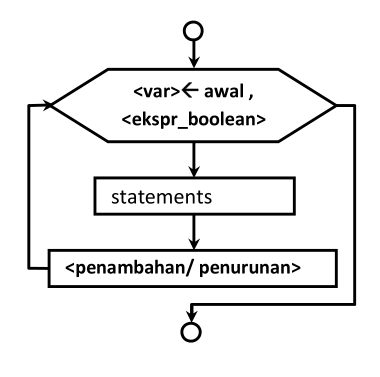
\includegraphics[width=8cm]{Capture2-8}
\caption{flowchart perulangan dengan for}
\end{figure}

\subsection{🔄 Perulangan dengan while}\label{perulangan-dengan-while}

Perulangan \textbf{while} digunakan untuk mengulangi perintah selama kondisi masih bernilai benar.

\subsubsection{Kapan Menggunakan while}

\begin{itemize}
\item Jumlah perulangan tidak diketahui
\item Perulangan berdasarkan kondisi tertentu
\item Perulangan yang berhenti ketika kondisi menjadi salah
\end{itemize}

\subsubsection{Sintaks while}

\lstinputlisting[language=c++, numbers=none]{../code/control-while-syntax.cpp}

\subsubsection{Cara Kerja while}

\begin{itemize}
\item Program mengecek kondisi sebelum masuk perulangan
\item Jika kondisi benar, kode dalam blok dijalankan
\item Setelah kode selesai, kondisi dicek lagi
\item Perulangan berhenti ketika kondisi menjadi salah
\end{itemize}

\begin{figure}[htbp]
\centering
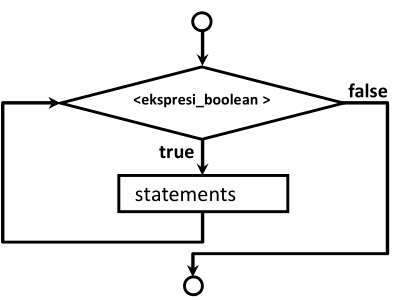
\includegraphics[width=8cm]{Capture2-9}
\caption{flowchart perulangan dengan while}
\end{figure}

\subsection{🔄 Perulangan dengan do-while}\label{perulangan-dengan-do-while}

Perulangan \textbf{do-while} mirip dengan while, tetapi kondisi dicek di akhir perulangan. Ini berarti kode minimal akan dijalankan sekali.

\subsubsection{Kapan Menggunakan do-while}

\begin{itemize}
\item Ketika kode minimal harus dijalankan sekali
\item Perulangan yang kondisi pengecekannya di akhir
\item Menu atau input yang perlu diproses minimal sekali
\end{itemize}

\subsubsection{Sintaks do-while}

\lstinputlisting[language=c++, numbers=none]{../code/control-do-while-syntax.cpp}

\subsubsection{Cara Kerja do-while}

\begin{itemize}
\item Program menjalankan kode dalam blok do terlebih dahulu
\item Setelah kode selesai, kondisi dicek
\item Jika kondisi benar, perulangan dilanjutkan
\item Jika kondisi salah, perulangan berhenti
\end{itemize}

\begin{figure}[htbp]
\centering
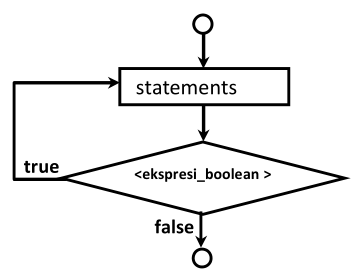
\includegraphics[width=8cm]{Capture2-10}
\caption{flowchart perulangan dengan do\dots while}
\end{figure}

\subsection{📊 Perbandingan while vs do-while}

\begin{center}
\begin{tabular}{|l|l|l|}
\hline
\textbf{Aspek} & \textbf{while} & \textbf{do-while} \\
\hline
Pengecekan kondisi & Di awal & Di akhir \\
\hline
Minimal eksekusi & 0 kali & 1 kali \\
\hline
Kapan digunakan & Kondisi mungkin salah di awal & Kode harus dijalankan minimal sekali \\
\hline
\end{tabular}
\end{center}

\subsubsection{Perbedaan Utama}

\begin{itemize}
\item \textbf{while}: kondisi dicek sebelum masuk perulangan
\item \textbf{do-while}: kondisi dicek setelah menjalankan kode
\item \textbf{while}: mungkin tidak menjalankan kode sama sekali
\item \textbf{do-while}: minimal menjalankan kode sekali
\end{itemize}

\subsection{⏭️ Kata Kunci break dan continue}\label{kata-kunci-continue-dan-break}

Kata kunci \textbf{break} dan \textbf{continue} digunakan untuk mengontrol aliran perulangan.

\subsubsection{Kata Kunci break}

\begin{itemize}
\item \textbf{break} menghentikan perulangan secara total
\item Program keluar dari perulangan dan melanjutkan ke baris setelah perulangan
\item Bisa digunakan dalam for, while, do-while, dan switch
\end{itemize}

\subsubsection{Kata Kunci continue}

\begin{itemize}
\item \textbf{continue} melompati iterasi saat ini
\item Program melanjutkan ke iterasi berikutnya
\item Kode setelah continue dalam iterasi yang sama tidak dijalankan
\end{itemize}

\subsubsection{Sintaks break dan continue}

\lstinputlisting[language=c++]{../code/02-control-statement-code-1.c++}

\subsection{💡 Contoh Program break dan continue}

\begin{enumerate}
\item Buka Qt Creator dan buat project Qt Console Application baru dengan nama "contoh"
\item Tulis kode berikut:

\lstinputlisting[language=c++, caption=Contoh penggunaan break dan continue, label=contoh2-5]{../code/contoh2-5.cpp}

\item Jalankan program dengan menekan Ctrl + R. Outputnya:

\begin{lcverbatim}
1 2 3 4 6 7 8 9 10
Loop berhenti karena break
\end{lcverbatim}
\end{enumerate}

\subsubsection*{Penjelasan Program}
\begin{itemize}
\item Program menggunakan perulangan for dari 1 sampai 10
\item Jika i == 5, program menggunakan continue untuk melompati angka 5
\item Jika i == 10, program menggunakan break untuk menghentikan perulangan
\item Hasilnya: angka 1-4, 6-9 ditampilkan, lalu loop berhenti
\end{itemize}

\section{🎯 Praktik Terbaik Control Statement}

\subsection{💡 Tips Menulis Control Statement yang Baik}

\begin{enumerate}
\item \textbf{Gunakan kondisi yang jelas} - Hindari kondisi yang membingungkan
\item \textbf{Tulis kode yang mudah dibaca} - Gunakan indentasi yang konsisten
\item \textbf{Hindari nested if yang terlalu dalam} - Maksimal 3-4 tingkat
\item \textbf{Gunakan switch untuk banyak pilihan} - Lebih efisien daripada if-else bertingkat
\item \textbf{Selalu gunakan kurung kurawal} - Meskipun hanya satu baris kode
\end{enumerate}

\subsection{⚠️ Kesalahan Umum yang Harus Dihindari}

\begin{itemize}
\item \textbf{Lupa break dalam switch} - Bisa menyebabkan fall-through
\item \textbf{Infinite loop} - Perulangan yang tidak pernah berhenti
\item \textbf{Kondisi yang selalu benar/salah} - Perulangan atau percabangan yang tidak efektif
\item \textbf{Indentasi yang salah} - Membuat kode sulit dibaca
\end{itemize}

\section{📊 Ringkasan Control Statement}

\subsection{🔄 Jenis-jenis Control Statement}

\begin{center}
\begin{tabular}{|l|l|l|}
\hline
\textbf{Jenis} & \textbf{Kegunaan} & \textbf{Contoh} \\
\hline
if & Percabangan sederhana & if (x > 0) \\
\hline
if-else & Percabangan dengan alternatif & if (x > 0) else \\
\hline
switch & Banyak pilihan & switch (x) case 1: \\
\hline
for & Perulangan dengan counter & for (int i=0; i<n; i++) \\
\hline
while & Perulangan dengan kondisi & while (x > 0) \\
\hline
do-while & Perulangan minimal sekali & do \{ \} while (x > 0) \\
\hline
break & Menghentikan perulangan & break; \\
\hline
continue & Melompati iterasi & continue; \\
\hline
\end{tabular}
\end{center}

\subsection{🎯 Kapan Menggunakan Setiap Jenis}

\begin{itemize}
\item \textbf{if}: Ketika ada satu kondisi yang perlu dicek
\item \textbf{if-else}: Ketika ada dua alternatif yang berbeda
\item \textbf{switch}: Ketika ada banyak pilihan berdasarkan nilai yang sama
\item \textbf{for}: Ketika jumlah perulangan sudah diketahui
\item \textbf{while}: Ketika jumlah perulangan tidak diketahui
\item \textbf{do-while}: Ketika kode minimal harus dijalankan sekali
\item \textbf{break}: Ketika perlu menghentikan perulangan secara paksa
\item \textbf{continue}: Ketika perlu melompati iterasi tertentu
\end{itemize}

\section{🔍 Latihan dan Soal}

\subsection{📝 Latihan 1: Program Kalkulator Sederhana}

Buat program kalkulator sederhana yang menerima dua angka dan operator (+, -, *, /) dari pengguna, kemudian menampilkan hasilnya.

\subsection{📝 Latihan 2: Program Menentukan Grade}

Buat program yang menerima nilai (0-100) dan menampilkan grade:
\begin{itemize}
\item A: 90-100
\item B: 80-89
\item C: 70-79
\item D: 60-69
\item E: 0-59
\end{itemize}

\subsection{📝 Latihan 3: Program Menampilkan Pola}

Buat program yang menampilkan pola bintang seperti berikut:
\begin{lcverbatim}
*
**
***
****
*****
\end{lcverbatim}

\section{📚 Referensi dan Bacaan Lanjutan}

Control statement adalah konsep fundamental dalam pemrograman yang telah dikembangkan sejak awal era komputer. Konsep ini pertama kali diperkenalkan dalam bahasa pemrograman FORTRAN pada tahun 1957\footnote{Backus, J. W. (1957). "The FORTRAN Automatic Coding System". Proceedings of the Western Joint Computer Conference.} dan kemudian dikembangkan lebih lanjut dalam bahasa ALGOL\footnote{Naur, P. (1960). "Report on the Algorithmic Language ALGOL 60". Communications of the ACM.}.

Dalam konteks C++, control statement mengikuti tradisi bahasa C yang dikembangkan oleh Dennis Ritchie di Bell Labs pada tahun 1972\footnote{Ritchie, D. M. (1993). "The Development of the C Language". ACM SIGPLAN Notices.}. Bjarne Stroustrup kemudian mengembangkan C++ dengan menambahkan fitur object-oriented programming sambil mempertahankan sintaks control statement yang familiar\footnote{Stroustrup, B. (1994). "The Design and Evolution of C++". Addison-Wesley.}.

Untuk pemahaman yang lebih mendalam tentang control statement dalam C++, pembaca dapat merujuk pada:

\begin{itemize}
\item \textbf{The C++ Programming Language} oleh Bjarne Stroustrup\footnote{Stroustrup, B. (2013). "The C++ Programming Language" (4th ed.). Addison-Wesley.}
\item \textbf{Effective C++} oleh Scott Meyers\footnote{Meyers, S. (2005). "Effective C++" (3rd ed.). Addison-Wesley.}
\item \textbf{C++ Primer} oleh Stanley Lippman\footnote{Lippman, S. B., Lajoie, J., \& Moo, B. E. (2012). "C++ Primer" (5th ed.). Addison-Wesley.}
\end{itemize}

\section{🎉 Kesimpulan}

Control statement adalah alat fundamental yang memungkinkan program untuk membuat keputusan dan mengulang operasi. Dengan menguasai konsep ini, Anda telah memiliki fondasi yang kuat untuk mengembangkan program yang lebih kompleks dan dinamis.

\begin{center}
\textbf{Selamat! Anda telah menguasai dasar-dasar Control Statement dalam C++} 🎯
\end{center}

\vspace{1cm}

\begin{center}
\textit{--- Bab selanjutnya: Array dan String ---}
\end{center}
	
	\chapter{Array dan String}\label{array-dan-string}
	\textbf{📋 Apa yang akan dipelajari}

Pada bab ini kita akan mempelajari tentang Array dan String dalam C++:

\begin{itemize}
\item Pengenalan Array dan cara kerjanya
\item Array 1 dimensi dan multi-dimensi
\item String dan operasinya
\item Manipulasi array dan string
\end{itemize}

\minitoc

\section{📊 Array (Larik)}\label{array}

\subsection{Apa itu Array?}

Array adalah tipe data terstruktur yang menyimpan sejumlah data dengan tipe yang sama dalam satu nama variabel.

\subsection{Karakteristik Array}

\begin{itemize}
\item \textbf{Tipe data sama} - semua elemen memiliki tipe data yang sama
\item \textbf{Jumlah tetap} - ukuran array ditentukan saat deklarasi
\item \textbf{Indeks} - setiap elemen diakses melalui indeks
\item \textbf{Memori berurutan} - elemen tersusun berurutan di memori
\end{itemize}

\subsection{Analoginya}

Array seperti \textbf{lemari dengan laci-laci}:
\begin{itemize}
\item Lemari = nama array
\item Laci = elemen array
\item Nomor laci = indeks array
\item Isi laci = nilai elemen
\end{itemize}

\subsection{Cara Kerja Array di Memori}

Array menyimpan data secara berurutan di memori komputer. Ketika array dideklarasikan, komputer mengalokasikan tempat yang berdekatan di memori.

\subsubsection{Ilustrasi Array di Memori}

Ilustrasi array satu dimensi pada memori komputer seperti gambar \ref{gambar3-1}.

\begin{figure}[htbp]
\centering
\shadowimage[width=8cm]{Capture3-1}
\label{gambar3-1}
\caption{Ilustrasi array satu dimensi pada memori komputer}
\end{figure}

\subsubsection{Karakteristik Penyimpanan}

\begin{itemize}
\item \textbf{Berurutan} - elemen tersusun berurutan di memori
\item \textbf{Berdekatan} - alamat memori yang bersebelahan
\item \textbf{Jarak tetap} - jarak antar elemen sesuai ukuran tipe data
\item \textbf{Indeks dimulai dari 0} - elemen pertama memiliki indeks 0
\end{itemize}

\subsubsection{Contoh Ukuran Memori}

\begin{itemize}
\item \textbf{int} - jarak antar elemen 2-4 byte
\item \textbf{char} - jarak antar elemen 1 byte
\item \textbf{double} - jarak antar elemen 8 byte
\end{itemize}

\subsection{📊 Array 1 Dimensi}\label{array-1-dimensi}

Array 1 dimensi adalah array yang memiliki satu indeks untuk mengakses elemennya.

\subsubsection{Cara Mengakses Array}

\begin{itemize}
\item \textbf{Berurutan} - mengakses elemen satu per satu
\item \textbf{Random} - mengakses elemen berdasarkan indeks tertentu
\item \textbf{Pengisian} - menyimpan nilai ke indeks tertentu
\item \textbf{Pengambilan} - membaca nilai dari indeks tertentu
\end{itemize}

\subsubsection{Analoginya}

Array 1 dimensi seperti \textbf{deretan kotak}:
\begin{itemize}
\item Setiap kotak memiliki nomor (indeks)
\item Kotak bisa diisi dengan barang (nilai)
\item Kita bisa mengambil barang dari kotak tertentu
\item Kita bisa mengisi barang ke kotak tertentu
\end{itemize}

\subsubsection{Deklarasi Array 1 Dimensi}\label{deklarasi-array-satu-dimensi}

\subsubsection{Sintaks Deklarasi}

\lstinputlisting[language=c++]{../code/03-array-string-code-1.c++}

\subsubsection{Komponen Deklarasi}

\begin{itemize}
\item \textbf{tipe\_data} - jenis tipe data elemen array (int, char, float, dll)
\item \textbf{nama\_array} - nama variabel array
\item \textbf{ukuran} - jumlah maksimal elemen array
\end{itemize}

\subsubsection{Contoh Deklarasi Array}

\lstinputlisting[language=c++]{../code/03-array-string-code-2.c++}

\subsubsection{Penjelasan Contoh}

\begin{description}
\item[\texttt{char huruf[9]}] 
Array karakter dengan 9 elemen (indeks 0-8), membutuhkan 9 byte memori

\item[\texttt{int umur[10]}] 
Array integer dengan 10 elemen (indeks 0-9), membutuhkan 40 byte memori

\item[\texttt{int kondisi[2] = \{0,1\}}] 
Array integer dengan 2 elemen yang langsung diinisialisasi:
\begin{itemize}
\item kondisi[0] = 0
\item kondisi[1] = 1
\end{itemize}

\item[\texttt{int arr\_dinamis[] = \{1,2,3\}}] 
Array dinamis dengan ukuran otomatis berdasarkan inisialisasi (3 elemen)
\end{description}

Tanda \texttt{{[}{]}} disebut juga ``elemen yang ke- ''. Misalnya
\texttt{kondisi{[}0{]}} berarti elemen yang ke nol. Array yang sudah
dipesan, misalnya 10 tempat tidak harus diisi semuanya, bisa saja hanya
diisi 5 elemen saja, baik secara berurutan maupun tidak. Namun pada
kondisi yang tidak sepenuhnya terisi tersebut, tempat pemesanan di
memori tetap sebanyak 10 tempat, jadi tempat yang tidak terisi tetap
akan terpesan dan dibiarkan kosong.

\subsubsection*{Contoh  Input dan Output Array}

Buatlah project baru dan tulis kode berikut:

\lstinputlisting[language=c++, caption=Input dan Output Array, label=contoh3-1]{../code/contoh2-1.cpp}

\textbf{Hasil:}
\begin{lcverbatim}
Memasukan nilai
Nilai Angka ke - 1 : 1
Nilai Angka ke - 2 : 2
Nilai Angka ke - 3 : 3
Nilai Angka ke - 4 : 4
Nilai Angka ke - 5 : 5
Membaca nilai:
Nilai Angka : 1
Nilai Angka : 2
Nilai Angka : 3
Nilai Angka : 4
Nilai Angka : 5
\end{lcverbatim}

\subsubsection*{Keterangan}

\begin{itemize}
\item
  Pada program diatas, kita membuat sebuah variabel array bernama
  \texttt{nilai} yang berisi \texttt{5} elemen bertipe \texttt{integer}.
  Kemudian untuk memasukkan nilai ke masing-masing elemen, digunakan
  perintah perulangan untuk mengakses indeksnya yang dimulai dari indeks
  ke \texttt{0}. Perulangan dilakukan dari indeks ke \texttt{0} sampai
  dengan indeks ke \texttt{4} (dalam hal ini
  \texttt{x\ \textless{}\ 5}). Mengapa sampai dengan indeks ke
  \texttt{4}? Hal ini karena \texttt{5} elemen array yang kita
  deklarasikan dimulai dari indeks ke \texttt{0}. Terdapat \texttt{5}
  elemen array, berarti indeks ke \texttt{0}, \texttt{1}, \texttt{2},
  \texttt{3}, dan \texttt{4}.
\item
  Setelah kita masukkan nilai ke masing-masing elemen, maka kita hanya
  perlu membaca datanya lagi, yaitu dengan melakukan perulangan kembali
  dengan cara mengakses indeks elemen-elemennya seperti pada saat kita
  memasukkan elemen-elemen tersebut kedalam \emph{array}. Perulangan
  untuk membaca isi elemen array juga diulang dari 0 sampai 4, yang
  artinya juga 5 elemen. Pada masing-masing perulangan tersebut,
  ditampilkan isi elemen ke layar dengan perintah
  \texttt{cout\textless{}\textless{}}.
\end{itemize}

\subsubsection*{Contoh  Manipulasi Array}

Buatlah project baru dan tulis kode berikut:

\lstinputlisting[language=c++, caption=Manipulasi Array, label=contoh3-2]{../code/contoh3-2.cpp}


\textbf{Hasil:}

\begin{lcverbatim}
elemen ke-1 ? 1
bil[0] = 1 dan alamatnya: 0x28fe68
bil[1] = 5 dan alamatnya: 0x28fe6c
bil[2] = 25 dan alamatnya: 0x28fe70
bil[3] = 50 dan alamatnya: 0x28fe74
bil[4] = 40 dan alamatnya: 0x28fe78
bil[5] = 50 dan alamatnya: 0x28fe7c
bil[6] = 60 dan alamatnya: 0x28fe80
\end{lcverbatim}

\subsubsection*{Keterangan}

\begin{itemize}

\item
  Program \ref{contoh3-2} memasukkan nilai-nilai integer kedalam array bernama
  bil yang berisi \texttt{7} elemen (dari indeks \texttt{0-6}).
\item
  Dalam array satu dimensi, suatu elemen array dapat diisi dengan isi
  elemen array pada indeks tertentu seperti pada contoh
  \texttt{bil{[}2{]}\ =\ bil{[}1{]}\ +\ 20;}. Pada contoh \ref{contoh3-2},
  \texttt{bil{[}2{]}} diisi dengan \texttt{bil{[}1{]}} yang berisi
  \texttt{25} ditambah dengan \texttt{20}, yaitu \texttt{55}.
\item
  Pada program \texttt{bil{[}3{]}\ =\ bil{[}bil{[}1{]}{]}}, artinya
  bilangan elemen ke-3 diisi dengan elemen array yang ke --
  \texttt{bil{[}1{]}}. Bilangan elemen ke-1, bernilai 5, yang berarti
  \texttt{bil{[}3{]}\ =\ bil{[}5{]}}. \texttt{Bil{[}5{]}} bernilai
  \texttt{50}, berarti \texttt{bil{[}3{]}\ =\ 50} juga.
\item
  Terlihat bahwa jarak antar elemen array \texttt{bil} berjarak
  \texttt{4\ bytes}.
\item
  Cara untuk menampilkan alamat \emph{array} adalah dengan menggunakan
  operator \texttt{\&}.
\end{itemize}
\begin{quotation}
{\LARGE \ding{46}} \textbf{TIPS} 

Dalam
bahasa C++, tidak terdapat \emph{error handling} terhadap batasan nilai
indeks, apakah indeks tersebut berada di dalam indeks array yang sudah
didefinisikan atau belum. Hal ini merupakan tanggung jawab programmer.
Sehingga jika programmer mengakses indeks yang salah, maka nilai yang
dihasilkan akan berbeda atau rusak karena mengakses alamat memori yang
tidak sesuai.
\end{quotation}
 

\subsubsection*{Contoh  Penanganan Batas Indeks Elemen Array}

Buatlah program beikut ini:

\lstinputlisting[language=c++, caption=Penanganan Batas Indeks Elemen Array, label=contoh3-3]{../code/contoh3-3.cpp}

\subsubsection*{Hasil dan Keterangan.}

\begin{itemize}

\item
  Progarm akan HANG-UP. Hal ini terjadi karena compiler tidak
  bertanggungjawab dengan pengaksesan indeks array yang melebihi batas
  yang dipesankan di memory.
\item
  Mengapa kompiler tidak menampilkan error pada saat kompilasi? Hal ini
  karena secara sintaks, program diatas tidaklah memiliki error
  penulisan. Error yang terjadi pada program diatas adalah runtime
  error, yaitu error yang terjadi / yang bisa dideteksi saat program
  sudah berjalan!
\end{itemize}

\subsection{Inisialisasi Array Satu Dimensi}\label{inisialisasi-array-satu-dimensi}

Array satu dimensi dapat diisi secara langsung ditulis pada program.
Pengisian data seperti itu sering disebut dengan inisialisasi data
array. Cara menginisialisasi data pada array adalah dengan menuliskannya
secara langsung pada source code program. Berikut contohnya:

\lstinputlisting[language=c++]{../code/03-array-string-code-3.c++}

Pada contoh diatas, semua elemen array bertipe integer yang berjumlah 5
buah tersebut diisi dengan nilai 0 semuanya. Cara lain menginisialisasi
array satu dimensi adalah sebagai berikut:

\lstinputlisting[language=c++]{../code/03-array-string-code-4.c++}

Nah, bagaimana jika kita ingin menginisialisasi elemen terakhirnya saja?
Kita tidak bisa melakukannya secara langsung. Yang harus dilakukan
adalah dengan menginisialisasinya satu-persatu seperti contoh berikut:

\lstinputlisting[language=c++]{../code/03-array-string-code-5.c++}

Pada contoh diatas, elemen terakhir diinilisasi dengan nilai 6. Kita
tidak bisa langsung mengisi dengan cara
\texttt{int\ IntegerArray{[}5{]}\ =\ \{6\}}, karena jika di isi dengan
cara demikian, maka isi elemen indeks ke-0 bernilai 6, sedangkan elemen
lainnya bernilai 0.

\subsubsection*{Contoh  Inisialisasi Array dengan nilai \textbackslash{}0}

Buatlah program berikut:

\lstinputlisting[language=c++, caption=Inisialisasi Array dengan nilai \textbackslash{}0, label=contoh3-4]{../code/contoh3-4.cpp}

\textbf{Hasil:}

\begin{lcverbatim}
Elemen ke-0: 0
Elemen ke-1: 1
Elemen ke-2: 2
Elemen ke-3: 3
Elemen ke-4: 4
Elemen ke-5: 5
Elemen ke-6: 6
\end{lcverbatim}

\subsubsection*{Keterangan}

Pada program diatas elemen array bernama bil yang dipesan sebanyak 7
elemen, di inisialisasi dengan nilai 0. Setelah di inisialisasi dengan
nilai 0, maka semua elemen array tersebut juga akan berisi dengan nilai
0. Hal ini dibuktikan dengan cara perulangan semua elemen array dan
ditampilkan dengan \texttt{cout}.

\subsubsection*{Contoh  Inisialisasi Array dua nilai elemen pertama}

Buka Qt Creator dan buat project Qt Console Application baru dengan
nama contoh \ref{contoh3-1}, kemudian tulis kode berikut.

\lstinputlisting[language=c++, caption=Inisialisasi Array dua nilai elemen pertama, label=contoh3-5]{../code/contoh3-5.cpp}

\textbf{Hasil:}

\begin{lcverbatim}
Elemen ke-0: 2
Elemen ke-1: 5
Elemen ke-2: 0
Elemen ke-3: 0
Elemen ke-4: 0
Elemen ke-5: 0
Elemen ke-6: 0
\end{lcverbatim}

\subsubsection*{Keterangan}

Inisialisasi elemen array dapat dilakukan hanya pada dua elemen pertama
saja, hal ini dilakukan dengan cara memberikan dua nilai pertama,
selanjutnya semua elemen lainnya yang tidak di inisialisasi secara
otomatis bernilai 0.

\begin{quotation}
{\LARGE \ding{46}} \textbf{TIPS}

Untuk
semua array pada C++, inisialisasi satu buah elemen saja pada array akan
membuat semua elemen array lainnya berisi nilai 0.
\end{quotation}
 

\textbf{Contoh:}

\lstinputlisting[language=c++]{../code/03-array-string-code-6.c++}

Maka hasilnya adalah:

\lstinputlisting[language=c++]{../code/03-array-string-code-7.c++}

Pada array satu dimensi, kita tidak dapat melakukan inisialisasi pada
array melebihi batas jumlah elemen array yang dipesan.

Pada array satu dimensi, kita juga dapat membuat array 1 dimensi tanpa
menyebutkan jumlah elemen array yang dipesan. Namun perlu di ingat bahwa
semua elemen harus di inisialisai terlebih dahulu.

Contoh:

\lstinputlisting[language=c++]{../code/03-array-string-code-8.c++}

\subsubsection*{Contoh  Tanpa inisialisasi, array langsung ditampilkan}

Tulislah program berikut ini:

\lstinputlisting[language=c++, caption=Tanpa inisialisasi array langsung ditampilkan, label=contoh3-6]{../code/03-array-string-contoh3-6.c++}

\textbf{Hasil:}

\begin{lcverbatim}
Elemen ke-0: 2
Elemen ke-1: 5
Elemen ke-2: 0
Elemen ke-3: 0
Elemen ke-4: v
\end{lcverbatim}

\subsubsection*{Keterangan}

Pada program C++, elemen array yang sudah dipesan dimemory pasti sudah
berisi data. Namun nilai datanya bersifat acak. Sehingga jika kita
mendeklarasikan sebuah elemen array tanpa di inisialisasi, maka nilai
masing-masing elemen akan bersifat acak juga seperti pada hasil program
diatas. Untuk itulah inisialisasi elemen array sangatlah penting.

\begin{quotation}
{\LARGE \ding{46}}  \textbf{TIPS}
 
 Inisialisasi pada elemen array yang dideklarsikan \textbf{SANGATLAH
 PENTING} untuk menghindari nilai \textbf{ACAK}!
\end{quotation}


\subsubsection*{Contoh  Penggunaan tipe data enum pada Array satu dimensi}

Buatlah program berikut:

\lstinputlisting[language=c++, caption=Penggunaan tipe data enum pada Array satu dimensi, label=contoh3-7]{../code/03-array-string-contoh3-7.c++}

\textbf{Hasil:}

\begin{lcverbatim}
Nilai hari selasa adalah = 30
\end{lcverbatim}

\subsubsection*{Keterangan.}

Pada program diatas, kita membuat sebuah tipe data enum bernama Hari
yang memiliki 7 elemen. Masing-masing elemen \texttt{enum} sama saja
seperti indeks array yaitu \texttt{0-6}. Kemudian kita membuat sebuah
array bernama \texttt{ArrayHari} yang berisi 7 elemen juga dan berisi
nilai \texttt{10-70}. Karena kita memanggil \\
\texttt{ArrayHari{[}Selasa{]}} berarti sama artinya dengan
\texttt{ArrayHari{[}2{]}}. Mengapa 2? Karena indeks Selasa adalah 2.
Sehingga muncullah output berupa 30, karena 30 berada pada indeks ke-2
dari \texttt{ArrayHari}.

Arti dari program diatas menunjukkan kita dapat mengakses indeks
\emph{array} dengan menggunakan \texttt{tipe\ data\ enum}, karena tipe
data \texttt{enum} pada kenyataannya akan dikonversikan kedalam nilai
\texttt{integer}, mulai dari \texttt{0}.

\subsection{Pengalamatan dan Pengkopian Array 1 Dimensi}\label{pengalamatan-dan-pengkopian-array-1-dimensi}

Array tidak bisa disalin begitu saja antara array satu yang ada nilainya
ke array lain yang kosong. Hal ini dikerenakan array bukanlah tipe data
primitif biasa. Array merupakan tipe data referensi dimana data yang
berada didalam elemen array berjumlah lebih dari satu buah dan diakses
dengan menggunakan alamat memory. Compiler C++ akan mencatat alamat
pertama dari indeks pertama array yang kita deklarasikan.

Contoh:

\lstinputlisting[language=c++]{../code/03-array-string-code-11.c++}

Maka variabel array data tersebut akan dicatat alamat elemen
\texttt{data{[}0{]}} pada memory. Jika kita mengakses elemen keduanya,
yaitu \texttt{data{[}1{]}}, maka compiler akan melakukan kalkulasi untuk
mendapatkan alamat \texttt{data{[}1{]}}, yaitu dengan cara menambahkan
alamat \texttt{data{[}0{]}} dengan lebar tipe data array yang kita
deklarasikan. Pada contoh diatas, kita membuat array bertipe integer.
Karena integer berukuran 4 byte, maka jika \texttt{data{[}0{]}}
beralamat di alamat \texttt{1000}, maka \texttt{data{[}1{]}} beralamat
di \texttt{1000\ +\ 4\ =\ 1004} dan seterusnya.

Lalu bagaimana cara mengkopikan isi elemen array dari satu variabel ke
variable array 1 dimensi lainnya? Kita harus menggunakan cara manual,
yaitu mengkopikan masing-masing elemennya satu persatu dengan perulangan
manual sesuai dengan jumlah elemen array yang dibuat.

\subsubsection*{Contoh  Percobaan Penyalinan Array 1 dimensi}

Buatlah program berikut:

\lstinputlisting[language=c++, caption=Percobaan Penyalinan Array 1 dimensi, label=contoh3-8]{../code/03-array-string-contoh3-8.c++}

\textbf{Hasil:}

\begin{figure}[htbp]
\centering
\shadowimage[width=8cm]{Capture3-8}

\end{figure}

\subsubsection*{Keterangan}

Program tidak bisa dijalankan karena terdapat \textbf{error}, bahwa
array tidak bisa dilakukan operasi assigment. Artinya kita tidak bisa
mengkopi antar array begitu saja.

\subsubsection*{Contoh  Penyalinan Array 1 dimensi dengan Perulangan}

Buatlah program berikut ini:

\lstinputlisting[language=c++, caption=Penyalinan Array 1 dimensi dengan Perulangan, label=contoh3-9]{../code/03-array-string-contoh3-9.c++}

\textbf{Hasil:}

\begin{lcverbatim}
1
2
3
4
5
6
\end{lcverbatim}

\subsubsection*{Keterangan}

\begin{itemize}

\item
  Cara penyalinan array adalah dengan melakukan perulangan sebanyak
  elemen array yang akan disalin dan menyalinnya secara manual
  satu-persatu pada indeks yang sama.
\item
  Kemudian ditampilkan sesuai dengan indeksnya. Elemen array yang
  dikopikan masih tetap memiliki array yang asli. Untuk menghapusnya,
  maka harus dilakukan secara manual.
\end{itemize}

\subsection{Array Multi Dimensi}\label{array-multi-dimensi}

Array multi dimensi berarti array yang kita deklasaikan dapat
dikembangkan ke array dimensi 2 dan seteruanya. Array multi dimensi
merupakan topik yang menarik dalam matematika. Setiap dimensi dalam
array direpresentasikan sebagai sub bagian dalam array. Oleh karena itu,
array dua dimensi array memiliki dua sub bagian, sebuah array
tiga-dimensi memiliki tiga sub bagian dan sebagainya. Sebuah contoh
bentuk nyata yang baik dari array dua dimensi adalah sebuah papan catur.
Satu dimensinya merupakan delapan baris, sedangkan dimensi lainnya
merupakan delapan kolom.

Contoh deklarasi array dua dimensi yang menggambarkan papan catur
adalah:

\lstinputlisting[language=c++]{../code/03-array-string-code-14.c++}

yang digambarkan dalam bentuk gambar \ref{fig:gambar3-2}.

\begin{figure}[htbp]
\centering
\shadowimage[width=8cm]{Capture3-11}
\caption{Contoh deklarasi array dua dimensi yang menggambarkan papan catur}
\label{fig:gambar3-2}
\end{figure}

Array dua dimensi sering kali digambarkan/dianalogikan sebagai sebuah
matriks atau bentuk grid. Jika array berdimensi satu hanya terdiri dari
1 baris dan banyak kolom, array berdimensi dua terdiri dari banyak baris
dan banyak kolom yang bertipe sama. Ilustrasi array dua dimensi dapat
dilihat sebagai berikut.

Berikut adalah gambar array berdimensi (baris x kolom = 3 x 4)

\begin{figure}[htbp]
\centering
\shadowimage[width=8cm]{Capture3-12}
\label{gambar3-3}
\caption{array dimensi 3 x 4}
\end{figure}

\subsection{Deklarasi Array Dua Dimensi}\label{deklarasi-array-dua-dimensi}

\lstinputlisting[language=c++]{../code/03-array-string-code-15.c++}

\textbf{Contoh:}

\lstinputlisting[language=c++]{../code/03-array-string-code-16.c++}

Array dua dimensi dapat mewakili bentuk suatu matriks, contoh matriks:


$x=
\begin{bmatrix}
8 &5& 9 & 6 & \\
8 & 2 & 1 & 0
\end{bmatrix}$

selanjutnya dapat dideklarasikan sebagai berikut:

\lstinputlisting[language=c++]{../code/03-array-string-code-17.c++}

atau diklarasikan dengan langsung menginisialisasi nilai
elemen-elemen-nya sebagai berikut:

\lstinputlisting[language=c++]{../code/03-array-string-code-18.c++}

Selanjutnya larik dua dimensi x dapat digambarkan sebagai berikut:

\lstinputlisting[language=c++]{../code/03-array-string-code-19.c++}

Array dua dimensi dapat digunakan untuk menampung tipe data numerik atau
non numerik.

Berikut adalah berbagai bentuk pembuatan array dua dimensi dengan tipe
data numerik ataupun non numerik.

Array dua dimensi bertipe data numerik

\lstinputlisting[language=c++]{../code/03-array-string-code-20.c++}

Jika data array integer yang diinputkan kurang dari deklarasi

\lstinputlisting[language=c++]{../code/03-array-string-code-21.c++}

Maka tiga data yang kurang akan diisi dengan angka 0

Array 2 dimensi dapat juga digunakan untuk menyimpan data karakter
(character). Pendeklarasian array 2 dimensi character adalah sebagai
berikut:

\lstinputlisting[language=c++]{../code/03-array-string-code-22.c++}

Akan ditampilkan sebagai:

\begin{tabular}{|c|c|c|c|c|}
\hline
A &B &C& D& E \\ \hline
F &G &H &I& J \\ \hline
K &L &M& N& O \\ \hline

\end{tabular}

Array 2 dimensi juga dapat dideklarasikan sebagai berikut:

\lstinputlisting[language=c++]{../code/03-array-string-code-23.c++}

Array diatas akan ditampilkan sebagai:

\begin{tabular}{|c|c|c|c|c|c|c|c|c|c|c|}
\hline
J & a & k & a & r & t & a & \textbackslash{0} & & & \\ \hline
B & a & n & d & u & n & g & \textbackslash{0} & & & \\ \hline
S & u & r & a & b & a & y & a &\textbackslash{0}  & &\\ \hline
S & e & m & a & r & a & n & g & \textbackslash{0} & & \\ \hline
Y & o & g & y & a & k & a & r & t & a &   \textbackslash{0} \\ \hline

\end{tabular}


Jika jumlah nilai character lebih banyak daripada deklarasi

\lstinputlisting[language=c++]{../code/03-array-string-code-24.c++}

{\LARGE \ding{55}}  Akan terjadi ERROR!

\begin{figure}[htbp]
\centering
\shadowimage[width=8cm]{Capture3-10}

\end{figure}

Jika data array character yang diinputkan kurang dari deklarasi

\lstinputlisting[language=c++]{../code/03-array-string-code-25.c++}

Maka tiga data yang kurang akan diisi dengan karakter NULL atau `\textbackslash{}0'

Jika data array integer yang diinputkan lebih dari deklarasi

\lstinputlisting[language=c++]{../code/03-array-string-code-26.c++}

{\LARGE \ding{55}} Matriks yang jumlah datanya lebih akan menyebabkan ERROR


\begin{figure}
\centering
\shadowimage[width=8cm]{Capture3-9}
\end{figure}




Array 2 dimensi juga dapat dideklarasikan secara dinamis. Dinamis bisa
dilakukan pada baris array 2 dimensi. Namun kita tidak bisa
mendeklarasikan array 2 dimensi secara dinamis pada kolom. Contoh
pendeklarasian baris dinamis adalah :

\lstinputlisting[language=c++]{../code/03-array-string-code-27.c++}

Akan ditampilkan sebagai:

\begin{tabular}{|c|c|c|c|c|}
\hline
5&12&17&10&7 \\ \hline
15&6&25&2&19 \\ \hline
4&9&20&22&11 \\ \hline
\end{tabular}


Contoh matriks dengan deklarasi baris dinamis lainnya:

\lstinputlisting[language=c++]{../code/03-array-string-code-28.c++}

Pada contoh diatas, jika kita hitung jumlah datanya adalah 18 buah,
padahal jika kita bagi per lima kolom, maka data 18 akan lebih 3 buah
(18/5 = 3). Sehingga secara otomatis terdapat 3 baris dan sisa 3 buah
data berikutnya akan membuat baris baru. Array dua dimensi tersebut akan
ditampilkan sebagai:


\begin{tabular}{|c|c|c|c|c|}
\hline
5 & 12 & 17 & 10 & 7 \\ \hline
15 & 6 & 25 & 2 & 19 \\ \hline
4 & 9 & 20 & 22 & 11 \\ \hline
77 & 88 & 99 & 0 & 0 \\ \hline

\end{tabular}

\subsubsection{Pengaksesan Array 2 Dimensi}\label{pengaksesan-array-2-dimensi}

Pengaksesan elemen-elemen array 2 dimensi dilakukan dengan cara
perulangan. Perulangan yang dilakukan harus disesuaikan dengan jumlah
dimensinya. Maka array 2 dimensi berarti perulangan yang dilakukan harus
dua kali. Terdapat outer loop yang digunakan untuk mengakses baris array
2 dimensi, dan inner loop yang digunakan untuk mengakses kolom array 2
dimensi.

\subsubsection*{Contoh  Deklarasi dan Menampilkan Array 2 Dimensi}

Buatlah program berikut:

\lstinputlisting[language=c++, caption=Deklarasi dan Menampilkan Array 2 Dimensi, label=contoh3-10]{../code/03-array-string-contoh3-10.c++}

\textbf{Hasil:}

\begin{lcverbatim}
51217107
15625219
4 91 52
\end{lcverbatim}


\subsubsection*{Keterangan}

Program diatas mendeklarasikan sebuah variabel array 2 dimensi bernama
matriks berukuran 3 baris dan 5 kolom. Kemudian matriks tersebut
langsung diinisialisasi dengan data integer sejumlah 15 data. Setelah
diinisialisasi kemudian dilakukan pengaksesan terhadap array 2 dimensi
tersebut dengan cara melakukan dua buah perulangan. Perulangan pertama
disebut outer loop yang digunakan untuk mengakses indeks baris variabel
matriks, sedangkan perulangan kedua disebut inner loop yang digunakan
untuk mengakses indeks kolom variabel matriks. Kemudian untuk
menampilkan data nya digunakan perintah cout dan untuk setiap data
elemen array diberikan karakter tab yang digunakan untuk memberi jarak
antar output data. Karakter tab pada bahasa C menggunakan escape
character `\textbackslash{}t'.

\subsubsection*{Contoh  Penyalinan Array 2 Dimensi ke Array 2 Dimensi lainnya}

Misalkan terdapat array 2 dimensi sebagai berikut
matriks\texttt{{[}3{]}{[}5{]}}

\begin{tabular}{|c|c|c|c|c|}
\hline
1 & 2 & 3 & 4 & 5 \\ \hline
6 & 7 & 8 & 9 & 10 \\ \hline
11 & 12 & 13 & 14 & 15 \\ \hline

\end{tabular}

Buatlah program berikut:

\lstinputlisting[language=c++, caption=Penyalinan Array 2 Dimensi ke Array 2 Dimensi lainnya, label=contoh3-11]{../code/03-array-string-contoh3-11.c++}

\textbf{Hasil:}

\begin{lcverbatim}
12345
678910
1112131416
\end{lcverbatim}

\subsubsection*{Keterangan}

Program diatas menyalin data dari matriks 2 dimensi ke matriks 2 dimensi
lainnya dengan menggunakan perulangan bertingkat. Perulangan bertingkat
memiliki 2 buah loop, yang pertama (\emph{outer loop}) digunakan untuk
mengakses baris matriks, dan inner loop digunakan untuk mengakses kolom
matriks. Kemudian untuk masing-masing elemen matriks dimasukkan kedalam
variabel array matrikshasil tepat pada baris dan kolom yang sesuai.

\subsubsection*{Contoh  Penyalinan array 2 dimensi ke dalam array 1 dimensi.}

Buatlah program berikut ini:

\lstinputlisting[language=c++, caption=Penyalinan array 2 dimensi ke dalam array 1 dimensi, label=contoh3-12]{../code/03-array-string-contoh3-12.c++}

\textbf{Hasil:}

\begin{lcverbatim}
1
2
3
4
5
6
7
8
9
10
11
12
13
14
15
\end{lcverbatim}

\subsubsection*{Keterangan}

\begin{itemize}

\item
  Untuk menyalin array 2 dimensi ke 1 dimensi, maka harus diperlukan
  sebuah array 1 dimensi baru yang berukuran total sesuai dengan hasil
  perkalian antara ukuran baris matriks dua dimensi dikalikan kolomnya.
  Misal array 2 dimensi berukuran 3 x 5, maka harus dibuat array 1
  dimensi berukuran minimal 15.
\item
  Kemudian untuk mengkopikan dari array 2 dimensi matriks ke array 1
  dimensi matrikshasil, harus dilakukan perulangan sesuai dengan baris
  dan kolom matriks. Indeks array matrikshasil diperoleh dari penambahan
  nilai counter yang diinisialisasi dari -1, dan berjalan mulai dari 0
  sampai dengan 14.
\end{itemize}

\subsection{Akses Array 2 dimensi}
 
Cara Pengaksesan Array dapat dilakukan dengan 2 cara:

\begin{enumerate}
\item Pengaksesan Baris demi Baris

Cara ini menelusuri elemen array dua dimensi per dimulai dari baris
pertama lalu kekanan sesuai dengan jumlah kolomnya. Setelah eleman dalam
baris tersebut habis, maka penelusuran akan berganti baris ke baris
berikutnya dan demikian seterusnya. Cara ini membutuhkan 2 buah loop,
dimana outer loop digunakan untuk mengakses indeks baris, dan inner loop
digunakan untuk mengakses indeks kolom.

Berikut adalah contohnya:

\lstinputlisting[language=c++, caption=Pengaksesan Baris demi Baris, label=contoh3-13]{../code/03-array-string-contoh3-13.c++}

\textbf{Hasil:}

\begin{lcverbatim}
1 2 3
4 5 6
\end{lcverbatim}

\item Pengaksesan Kolom demi Kolom

Cara ini menelusuri elemen array dua dimensi per dimulai dari kolom
pertama lalu kebawah sesuai dengan jumlah barisnya. Setelah eleman dalam
kolom tersebut habis, maka penelusuran akan berganti kolom ke kolom
berikutnya dan demikian seterusnya. Cara ini membutuhkan 2 buah loop,
dimana outer loop digunakan untuk mengakses indeks kolom, dan inner loop
digunakan untuk mengakses indeks baris.

\textbf{Contoh:}

\lstinputlisting[language=c++, caption=Pengaksesan Kolom demi Kolom, label=contoh3-14]{../code/03-array-string-contoh3-14.c++}

\textbf{Hasil:}

\begin{lcverbatim}
1 4
2 5
3 6
\end{lcverbatim}

\end{enumerate}







\section{String}\label{string}

\index{String}String adalah kumpulan dari nilai-nilai karakter yang berurutan dalam
bentuk satu dimensi, nilai string ini haruslah ditulis didalam tanda
petik dua (") misalnya: ``ini string''. Suatu nilai string disimpan di
memori dengan diakhiri oleh nilai ``\textbackslash{}''0(null), misalnya nilai string
``ANTO'' disimpan dimemori dalam bentuk

\begin{tabular}{|c|c|c|c|c|}
\hline
A & N & T & 0 & \textbackslash{0}\\ \hline
\end{tabular}


Dengan mengetahui nilai string diakhiri oleh nilai `\textbackslash{}0', maka akhir
nilai dari suatu string dapat dideteksi.

Untuk mendeklarasikan sebuah string terdapat dua cara:

\begin{enumerate}


\item
  Menggunakan \index{array of character}array of character yang sering disebut 
  \index{C-style}C-style string
\item
  Menggunakan tipe data string pada C++
\end{enumerate}

\subsection{Array of Character}\label{array-of-character}

Cara menggunakan array of character sama seperti mendeklarasikan
variabel bertipe array namun bertipe data character seperti yang sudah
dijelaskan pada bagian-bagian sebelumnya. Array of character memiliki
sifat-sifat array lainnya yaitu bersifat statis dan letaknya berurutan
di dalam memory komputer. String berjenis array of character selalu
dibuat dengan menggunakan array satu dimensi yang dapat terdiri dari
karakter-karakter yang ditulis dengan menggunakan tanda petik tunggal
(') atau satu kesatuan string yang ditulis dengan tanda petik ganda
('').

\subsubsection*{Contoh pendeklarasian array of character}

\lstinputlisting[language=c++]{../code/03-array-string-code-34.c++}

Pada sebuah string, terdapat karakter \texttt{\textbackslash{}0} yang
dapat digunakan untuk mengetahui kapan berakhirnya suatu string. Berikut
adalah contoh penggunaaanya.

\subsubsection*{Contoh  Penggunaan karakter \textbackslash{0}}

Buatlah program berikut:

\lstinputlisting[language=c++, caption=Penggunaan karakter \textbackslash{0, label=contoh3-15]{../code/03-array-string-contoh3-15.c++}

\textbf{Hasil:}

\begin{lcverbatim}
String
\end{lcverbatim}

\subsubsection*{Keterangan}

Program diatas dapat mengetahui kapan berakhirnya suatu string, dalam
arti kita dapat mengetahui panjang suatu string dengan melakukan
perulangan untuk setiap karakter yang ada pada array sampai ditemukannya
katakter `\textbackslash{}0'.

\subsubsection*{Contoh  String tanpa karakter \textbackslash{0}}

Buatlah program berikut:

\lstinputlisting[language=c++, caption=String tanpa karakter \textbackslash{0, label=contoh3-16]{../code/03-array-string-contoh3-16.c++}

\textbf{Hasil:}

\begin{figure}[htbp]
\centering
\shadowimage[width=8cm]{Capture2-7}

\end{figure}

\subsubsection*{Keterangan}

Terlihat bahwa kita tidak bisa membuat array fa character tepat sesuai
dengan jumlah karakter yang kita inisialisasikan. Jika dilihat kata
``String'' berjumlah 6 huruf, sedangkan kita sudah mendeklarasikan
variabel \texttt{string{[}6{]}} namun ternyata jumlah elemennya masih
dianggap terlalu sedikit. Hal ini terjadi karena minimal kita harus
mengalokasikan sejumlah 7 buah elemen. Elemen ke-7 digunakan untuk
menyimpan tanda akhir string atau karakter \textbackslash0 tersebut.

\subsubsection*{Contoh  Mengisi Array of Character}

Buatlah program berikut:

\lstinputlisting[language=c++, caption=Mengisi Array of Character, label=contoh3-17]{../code/03-array-string-contoh3-17.c++}

\textbf{Hasil:}
\begin{lcverbatim}
Isi data string: Wachid
hasil data string: Wachid
\end{lcverbatim}


\subsubsection*{Keterangan}

\begin{itemize}

\item
  Pada program diatas kita mendeklarasikan variabel array of string
  bernama buffer yang berukuran 6 elemen. Variabel buffer diatas
  merupakan variabel berjenis string C-style yang diinisialisasi dengan
  karakter \textbackslash{0} atau karakter\index{NULL} NULL.
\item
  Problem lainnya adalah jika kita menginputkan data string yang
  mengandung spasi, maka cin hanya akan membaca data string sebelum
  spasi saja.
\end{itemize}

\textbf{Contoh:}

\lstinputlisting[language=c++]{../code/03-array-string-code-38.c++}

\subsubsection*{Contoh  Pengisian variabel array of character dengan maksimum jumlah karakter.}

Tulislah program berikut:

\lstinputlisting[language=c++, caption=Pengisian variabel array of character dengan maksimum jumlah
karakter, label=contoh3-18]{../code/03-array-string-contoh3-18.c++}

\textbf{Hasil:}
\begin{lcverbatim}
Isi data string: Nur Wachid
hasil data string: Nur Wachid
\end{lcverbatim}


\subsubsection*{Keterangan}

Pada contoh program diatas, kita menggunakan perintah
\texttt{cin.get(buffer,49)}. Perintah diatas ``memaksa'' agar perintah
\texttt{cin} mengambil semua data inputan ke dalam variabel buffer
sampai sejumlah 49 karakter. Jika karakter yang diinputkan lebih dari 50
karakter, maka otomatis karakter yang disimpan kedalam variabel buffer
hanyalah berjumlah 50 karakter pertama saja.

\section{Fungsi-fungsi String}\label{fungsi-fungsi-string}

Bahasa C++ menggunakan fungsi-fungsi pustaka yang disediakan untuk
mengoperasikan suatu nilai string yang dimasukkan dalam file header
string.h. Beberapa fungsi string yang terdapat pada header string.h
adalah sebagai berikut:

\lstinputlisting[language=c++]{../code/03-array-string-code-40.c++}

Berfungsi untuk menentukkan panjang suatu nilai string.

Bentuk umum:
\texttt{int\ strlen(\textless{}identifier\ string\textgreater{});}

\lstinputlisting[language=c++]{../code/03-array-string-code-41.c++}

Berfungsi untuk menentukan panjang suatu nilai tipe data class string

Bentuk umum method:
\texttt{\textless{}nama\_var\_string\textgreater{}.length();}

\subsubsection*{Contoh  Penggunaan fungsi strlen()}

Buatlah program berikut ini:

\lstinputlisting[language=c++, caption=Penggunaan fungsi strlen(), label=contoh3-19]{../code/03-array-string-contoh3-19.c++}

\textbf{Hasil:}

\begin{lcverbatim}
Masukkan kalimat apapun
yang anda sukai (max 100 huruf): Nur Wachid 
panjang huruf adalah: 10 karakter
\end{lcverbatim}
 

\subsubsection*{Keterangan}

Fungsi strlen menerima satu parameter yang hanya bertipe array of
character. Fungsi ini tidak bisa menerima parameter berupa tipe data C++
string.

\subsubsection*{Contoh  Penggunaan fungsi length pada tipe data string C++}

Buatlah program berikut ini:

\lstinputlisting[language=c++, caption=Penggunaan fungsi length pada tipe data string C++, label=contoh3-20]{../code/03-array-string-contoh3-20.c++}

\textbf{Hasil:}

\begin{lcverbatim}
Masukkan kalimat apapun yang anda sukai
(max 100 huruf): Nur Wachid 
panjang huruf adalah: 10 karakter
\end{lcverbatim}
 

\subsubsection*{Keterangan}

\begin{itemize}

\item
  Program diatas tidak menggunakan array of character, melainkan
  menggunakan tipe data C++ \texttt{class\ string}. Tipe data ini
  spesial karena berupa tipe data object oriented. Untuk menggunakan
  tipe data ini kita harus menginclude-kan
  \texttt{\#include\ \textless{}string\textgreater{}} pada bagian
  \emph{preprocessor directive}.
\item
  Kemudian untuk mengakses panjang karakternya digunakan method (fungsi)
  dari object string bernama \texttt{length()}. Fungsi \texttt{length}
  sama dengan fungsi \texttt{strlen} yaitu mengambil jumlah karakter
  dalam string tersebut.
\end{itemize}

\subsection{strcpy() dan strncpy()}\label{strcpy-dan-strncpy}

Dalam bahasa C++, untuk menyalin nilai suatu string tidak dapat langsung
menuliskannya seperti halnya kompiler lain, sehingga proses menyalin
atau mengerjakan suatu nilai string ke variabel string yang lain
diperlukan suatu fungsi pustaka yang bernama \texttt{strcpy()}.

\begin{enumerate}

\item
  Bentuk umum:
  \texttt{void\ strcpy(\textless{}stringhasil\textgreater{},\textless{}stringsumber\textgreater{});}
\item
  Bentuk umum:
  \texttt{void\ strncpy(\textless{}stringhasil\textgreater{},\textless{}stringsumber\textgreater{});}
\end{enumerate}

\subsubsection*{Contoh  Penggunaan fungsi strcpy()}

Buatlah program berikut ini:

\lstinputlisting[language=c++, caption=Penggunaan fungsi strcpy(), label=contoh3-21]{../code/03-array-string-contoh3-21.c++}

\textbf{Hasil:}
\begin{lcverbatim}
String pertama : STRING
String Kedua : STRING
\end{lcverbatim}


\subsubsection*{Keterangan}

\begin{itemize}
\item
  Program diatas digunakan untuk mengkopikan nilai dari array of
  character data ke data2 dengan menggunakan perintah \texttt{strcpy}.
  Hal itu terbukti dengan hasil akhir dimana string pertama dan kedua
  bernilai sama, yaitu ``STRING''.
\item
  Jika variabel sesumber lebih besar daripada variabel hasil,
  \texttt{trcpy\ ()} akan error karena melebihi buffer. Untuk melindungi
  hal ini, digunakan fungsi \texttt{strncpy\ ()} Fungsi ini dapat
  memberikan parameter jumlah maksimum karakter untuk penyalinan.
  \texttt{strncpy\ ()} akan menyalin sampai karakter null pertama atau
  jumlah maksimum. Contoh Error:

  \begin{itemize}
  
  \item
    \texttt{char\ data{[}5{]}\ =\ \{\textquotesingle{}\textbackslash{}0\textquotesingle{}\};}
  \item
    \texttt{char\ data2{[}{]}="STRING";}
  \end{itemize}
\item
  Hal ini terjadi karena data2 berjumlah 6 karakter, sedangkan data
  berjumlah 5 karakter. Jadi ketika data2 dikopikan ke data, maka akan
  terjadi error karena tempatnya kurang.
\end{itemize}

\subsubsection*{Contoh  Penggunaan fungsi strncpy()}

Buatlah program beriku:

\lstinputlisting[language=c++, caption=Penggunaan fungsi strncpy(), label=contoh3-22]{../code/03-array-string-contoh3-22.c++}

\textbf{Hasil:}
\begin{lcverbatim}
 String pertama : STRING
 String Kedua : STRINGKU
\end{lcverbatim}


\subsubsection*{Keterangan}

\begin{itemize}

\item
  Fungsi \texttt{strncpy} dapat digunakan untuk menyalin dari satu array
  of character ke array of character lainnya dengan memberikan penanda
  batas maksimal penyalinan. Pada contoh diatas, string ``STRINGKU''
  hendak disalin ke variabel data yang hanya berisi 6 elemen. Karena
  fungsi \texttt{strncpy} hanya dibatasi menyalin 5 karakter saja, maka
  yang tersalin adalah \texttt{STRIN} saja.
\item
  Karakter ke-6 pada variabel data digunakan untuk menyimpan karakter
 NULL atau \textbackslash0.
\end{itemize}

\subsection{strcat()}\label{strcat}

\textbf{Bentuk umum}:
\texttt{strcat(\textless{}string\ hasil\textgreater{},\ \textless{}string\ sumber\textgreater{});}

String dalam C++ tidak bisa digabungkan begitu saja dengan menggunakan
operator + seperti pada bahasa pemrograman Pascal. Jika dipaksakan
menggunakan operator + akan ditampilkan pesan kesalahan sebagai berikut
ini.

\subsubsection*{Contoh  Penggunaan fungsi strcat()}

Buatlah program beriku:

\lstinputlisting[language=c++, caption=Penggunaan fungsi strcat(), label=contoh3-23]{../code/03-array-string-contoh3-23.c++}

\textbf{Hasil:}

\begin{figure}[htbp]
\centering
\shadowimage[width=8cm]{Capture3-6}

\end{figure}

\subsubsection*{Keterangan}

Opearator + tidak bisa digunakan untuk menggabungkan dua buah string.
Untuk menggabungkan dua string, digunakan fungsi \texttt{strcat()}.

\subsubsection*{Contoh  Penggunaan fungsi strcat()}

Buatlah program berikut:

\lstinputlisting[language=c++, caption=Penggunaan fungsi strcat(), label=contoh3-24]{../code/03-array-string-contoh3-24.c++}

\textbf{Hasil:}

\begin{lcverbatim}
Jadi gabungannya adalah:
Kami kelompok belajar Qt C++
\end{lcverbatim}


\subsubsection*{Keterangan}

\begin{itemize}

\item
  Program diatas menggunakan fungsi \texttt{strcat} dimana fungsi
  tersebut akan menggabungkan dua buah string. Parameter string pertama
  juga digunakan untuk menampung string gabungan kedua string tersebut.
  Sehingga pada akhirnya variabel string1 lah yang ditampilkan ke layar.
\item
  Variabel \texttt{string1} diberi ukuran 100 karena jika tidak diberi
  ukuran elemen maka \texttt{string1} tidak bisa memperbesar ukurannya
  di memory komputer sehingga akan menyebabkan program \textbf{HANG}.
\end{itemize}

\begin{quotation}
{\LARGE \ding{46}} \textbf{TIPS}

Beberapa fungsi yang \texttt{\#include\ string.h} dan dapat digunakan
untuk memanipulasi \emph{array of character} adalah:

\emph{strrev()}

Bentuk umum: \texttt{strrev(string)}

Digunakan untuk membalik susunan string, misal: anton menjadi notna

\emph{strlwr()}

Bentuk umum: \texttt{strlwr(string)}

Digunakan untuk mengubah string menjadi huruf kecil semua

\emph{strupr}

Bentuk umum: \texttt{strupr(string)}

Digunakan untuk mengubah string menjadi huruf besar semua

\emph{strchr()}

Bentuk umum: \texttt{strchr(stringsumber,karakter\ yang\ dicari)}

Dalam bahasa C++ disediakan suatu fungsi pustaka yaitu \texttt{strchr()}
untuk mencari nilai suatu karakter yang ada di suatu string. Hasil dari
fungsi ini adalah alamat letak dari karakter pertama di nilai string
yang sama dengan karakter yang dicari.

\emph{strcmp()}

Bentuk umum: \texttt{strcmp(string1,string2);}

Untuk membandingkan dua nilai string tidak bisa menggunakan operator
hubungan, karena operator tersebut tidak untuk operasi string. Untuk
membandingkan dua nilai string kita gunakan fungsi pustaka
\texttt{strcmp()} dengan hasil sebagai berikut:

\begin{itemize}

\item
Hasil \textless{} 0, Jika string1 \textless{} string2
\item
Hasil = 0, Jika string1 = string2
\item
Hasil \textgreater{} 0, Jika string1 \textgreater{} string2
\end{itemize}
\end{quotation}


\subsection{Fungsi mengubah string menjadi numerik dan sebaliknya}\label{fungsi-mengubah-string-menjadi-numerik-dan-sebaliknya}

Pada bahasa C++ tipe data \emph{array of character} bisa dikonversi
menjadi \texttt{numerik} dan sebaliknya numerik bisa dikonversi menjadi
\texttt{array\ of\ character}. Caranya adalah
\texttt{\#include\ \textless{}stdlib\textgreater{}}. Fungsi-fungsi
konversi dari string ke numerik adalah:

\lstinputlisting[language=c++]{../code/03-array-string-code-48.c++}

Sedangkan kebalikannya, fungsi untuk mengubah numerik menjadi string
adalah:

\lstinputlisting[language=c++]{../code/03-array-string-code-49.c++}

Fungsi diatas menerima parameter
\texttt{\textless{}var\ numerik\textgreater{}},
\texttt{\textless{}var\ array\ of\ character\textgreater{}}, dan
\texttt{\textless{}basis\ bilangan\textgreater{}}

\subsection{Class string pada C++}\label{class-string-pada-c}

C++ library standar memiliki kelas string yang membuat bekerja dengan
string lebih mudah dengan menyediakan satu set encapsulasi dari data,
dan fungsi untuk memanipulasi data \index{String}string. Kelas ini dikenal dengan
\texttt{std::} string yang dapat menangani rincian alokasi memori dan
membuat kopi string, atau menempatkan mereka di memory dengan lebih
mudah.

\subsubsection*{Contoh  Pembuatan variabel string C++, penyalinan string, dan
penggabungan string}

Buatlah program berikut:

\lstinputlisting[language=c++, caption=Pembuatan variabel string C++ penyalinan string dan
penggabungan string, label=contoh3-25]{../code/03-array-string-contoh3-25.c++}

\textbf{Hasil:}

\begin{lcverbatim}
Isi str1 : Ini string C++
Isi str1 : Ini string C++
Isi str1 : Ini string C++
Halo, Ini string C++
\end{lcverbatim}

\subsubsection*{Keterangan}

\begin{itemize}

\item
  Tanpa perlu dipelajari lebih dalam, kita dapat melihat bahwa class
  string pada C++ jelas jauh lebih cepat penggunaannya dan mudah dalam
  pembuatan serta penyalinan seperti semudah mengoperasikan variabel
  bertipe integer saja. Demikian pula, \emph{concatenating}
  (penggabungan) dua string dapat dilakukan dengan hanya menambahkan
  mereka, sama juga seperti kita akan melakukan penjumlahan dengan
  integer apapun.
\item
  Syarat untuk dapat menggunakan class string adalah harus
  mengincludekan \texttt{\#include\ \textless{}string\textgreater{}},
  seperti yang dapat dilihat pada kode program diatas.
\end{itemize}
\begin{quotation}
{\LARGE \ding{46}}  \textbf{TIPS} 
 
 Class
 string memiliki beberapa fitur / manfaat, yaitu: 
\begin{itemize}
\item Mengurangi kesulitan dalam upaya penciptaan dan
memanipulasi string
\item Meningkatkan stabilitas aplikasi
yang sedang diprogram dalam pengelolaan dan alokasi memori internal
\item Mudah dalam menyalin, memotong, menemukan, dan
penghapusan string
\item Memberikan kesempatan pada
programmer untuk lebih fokus pada pengembangan aplikasi daripada
kesulitan dalam manipulasi string
\end{itemize} 
 
\end{quotation}


\subsubsection*{Contoh  Penggunaan class string untuk manipulasi data}

Buatlah program berikut:

\lstinputlisting[language=c++, caption=Penggunaan class string untuk manipulasi data, label=contoh3-26]{../code/03-array-string-contoh3-26.c++}

\textbf{Hasil:}

 \begin{lcverbatim}
 Halooooooo
 saya belajar
 C
 \end{lcverbatim}

\subsubsection*{Keterangan}

Dapat dilihat langsung pada baris komentar program diatas.

\subsubsection*{Contoh  Penggabungan string dengan menggunakan class string}

Buatlah program berikut:

\lstinputlisting[language=c++, caption=Penggabungan string dengan menggunakan class string, label=contoh3-27]{../code/03-array-string-contoh3-27.c++}

\textbf{Hasil:}
\begin{lcverbatim}
Percobaan 1 Percobaan 2
Percobaan 1 Percobaan 2 Percobaan 3 Percebaan tampung
\end{lcverbatim}


\subsubsection*{Keterangan}

\begin{itemize}

\item
  Pada program diatas, terdapat dua buah variabel bertipe string, yaitu
  \texttt{satu} dan \texttt{dua}. Tipe data string tidak mendukung
  penggabungan string dengan mudah yaitu dengan menggunakan operator +.
  Pada contoh diatas, variabel satu ditambah isinya dengan variabel dua
  dan disimpan kembali pada variabel satu. Sehingga variabel satu berisi
  string gabungan ``Percobaan 1 Percobaan 2''.
\item
  Kemudian dibuat suatu variabel tampung yang kemudian juga digabungkan
  kedalam variabel satu. Cara penggabungan (concatenation) string dapat
  dilakukan juga dengan cara kedua, yaitu dengan menggunakan
  \texttt{method\ append}. \texttt{Method\ append} ini dimiliki oleh
  semua variabel bertipe class string dan dapat langsung digunakan
  dengan memasukkan parameter bertipe string juga.
\end{itemize}

\subsubsection*{Contoh  Pengaksesan isi nilai class string}

Buatlah program berikut:

\lstinputlisting[language=c++, caption=Pengaksesan isi nilai class string, label=contoh3-28]{../code/03-array-string-contoh3-28.c++}

\textbf{Hasil:}

\begin{lcverbatim}
I
n
d
o
n
e
s
i
a


R
a
y
a

C-style: Indonesia Raya
\end{lcverbatim}

\subsubsection*{Keterangan}

\begin{itemize}

\item
  Variabel string yang bertipe class string juga memiliki sifat yang
  sama dengan variabel string dengan model C-string style. Keduanya
  merupakan gabungan dari karakter-karakter yang berbentuk array
  berdimensi satu. Sehingga jika kita memiliki variabel string satu
  seperti pada program, kita dapat mengakses semua elemen-elemen
  karakter penyusun string tersebut dengan menggunakan perulangan dan
  kemudian kita akses indeks dari masing-masing elemen array
  characternya.
\item
  Pada bagian kedua, kita juga bisa mengkonversi dari tipe data class
  string menjadi tipe data array of character atau tipe data C-style
  string dengan menggunakan method dari class string, yaitu
  \texttt{c\_str()}.
\end{itemize}

\subsubsection*{Contoh  Menemukan substring pada sebuah string besar}

Tulislah program berikut ini:

\lstinputlisting[language=c++, caption=Menemukan substring pada sebuah string besar, label=contoh3-29]{../code/03-array-string-contoh3-29.c++}

\textbf{Hasil:}

\begin{lcverbatim}
Contoh string adalah:
Kata pak Hari, "hari ini matahari cerah sekali!"
Ketemu pertama kata "hari" pada offset 16
Mencari semua kata substring "hari"
Kata "hari" ada di offset 16
Kata "hari" ada di offset 29
Mencari semua karakter 'a'
'a' ditemukan pada posisi 1
'a' ditemukan pada posisi 3
'a' ditemukan pada posisi 6
'a' ditemukan pada posisi 10
'a' ditemukan pada posisi 17
'a' ditemukan pada posisi 26
'a' ditemukan pada posisi 28
'a' ditemukan pada posisi 30
'a' ditemukan pada posisi 37
'a' ditemukan pada posisi 43
\end{lcverbatim}

\subsubsection*{Keterangan}

\begin{itemize}

\item
  Program diatas membuat sebuah variabel string bernama strSample yang
  diisi dengan kalimat : ``Kata pak Hari, ``hari ini matahari cerah
  sekali!''\,''. Kemudian program akan mencari kata ``hari'' yang
  pertama ditemukan pada kalimat tersebut dengan menggunakan method
  find(\texttt{\textless{}kata\ yang\ dicari\textgreater{}},\texttt{\textless{}posisi\ indeks\ dimulainya\ pencarian\textgreater{}}).
  Method ini bersifat case-sensitive sehingga kata ``Hari'' dengan
  ``hari'' berbeda. Pencarian dimulai dari huruf pertama, sehingga kata
  ``hari'' ditemukan pada huruf ke 16, bukan ke-9, karena karakter ke-9
  kata ``Hari'' menggunakan huruf besar.
\item
  Pencarian berikutnya adalah pencarian semua kata ``hari''. Karena kata
  ``hari'' ada lebih dari satu buah, maka pencarian harus diloop, karena
  method find membutuhkan indeks mulainya pencarian. Untuk setiap kata
  ``hari'' yang ditemukan, kemudian ditampilkan posisi indeksnya ke
  layar.
\item
  Selain dapat menerima parameter berupa substring, method find juga
  dapat menerima parameter berupa character dengan proses pencarian yang
  sama dengan proses pencarian dengan parameter substring.
\end{itemize}

\subsubsection*{Contoh  Membalik kata / kalimat.}

Tulislah program berikut ini:

\lstinputlisting[language=c++, caption=Membalik kata / kalimat, label=contoh3-30]{../code/03-array-string-contoh3-30.c++}

\textbf{Hasil:}

\begin{lcverbatim}
String asli:
String ini akan dibalik!
Setelah dibalik:
!kilabid naka ini gnirtS
\end{lcverbatim}

\subsubsection*{Keterangan}

Untuk membalik kalimat bertipe string, kita harus menggunakan \index{library}library
header \index{algoritm}algoritm, sehingga kita harus mengincludekan library tersebut
\texttt{\#include\ \textless{}algorithm\textgreater{}}. Setelah itu
untuk menggunakannya kita gunakan perintah
\emph{reverse}(\texttt{\textless{}indeks\ string\ pertam\textgreater{}},\texttt{\textless{}indeks\ string\ terakhir\textgreater{}}).
Perintah reverse tersebut akan benar-benar mengganti string asli menjadi
terbalik, sehingga variable string kita akan berubah berisi kalimat yang
sudah terbalik.

\subsubsection*{Contoh  Konversi huruf besar dan kecil.}

Tulislah program berikut ini:

\lstinputlisting[language=c++, caption=Konversi huruf besar dan kecil, label=contoh3-31]{../code/03-array-string-contoh3-31.c++}

\textbf{Hasil:}

\begin{lcverbatim}
Masukkan sebuah string:
Ini KoK tulisaNya AlaY BaNGet yA!
Hasil konversi ke huruf besar:
INI KOK TULISANYA ALAY BANGET YA!

Hasil konversi ke huruf kecil:
ini kok tulisanya alay banget ya!
\end{lcverbatim}

\subsubsection*{Keterangan}

Program diatas menunjukkan function transform pada library algoritm
dapat digunakan untuk mengkonversi string dari besar ke kecil dan dari
kecil ke besar.

	
	\chapter{Fungsi}
	\textbf{Agenda}

Pada Bab ini kita akan mempelajari tentang funtion bahasa C++ seperti berikut ini

\minitoc

Fungsi (Function) adalah sekumpulan program yang diberi nama, sehingga
dengan demikian jika program itu diperlukan dapat dipanggil kembali.
Walaupun Pemrograman Berorientasi Objek telah menggeser perhatian dari
fungsi ini, namun fungsi tetap saja merupakan bagian paling inti dalam
suatu program. Fungsi global bisa berada di luar kelas maupun objek.

Fungsi dapat melakukan manipulasi terhadap data dan dapat mengembalikan
suatu nilai. Semua program yang ditulis dengan bahasa C++ paling tidak
mempunyai sebuah fungsi, yaitu \texttt{main()}, fungsi ini akan
dipanggil secara otomatis ketika program dieksekusi, sedangkan fungsi
yang lain baru akan bekerja ketia fungsi tersebut dipanggil. Karena
fungsi ini bukan merupakan bagian dari objek, maka fungsi ini dipanggil
secara global, dapat diakses dari manapun dalam program yang ditulis

Setiap fungsi diberi nama, dan ketika dalam suatu program dijumpai nama
tersebut, maka eksekusi program akan dialihkan ke tubuh (isi) fungsi
tersebut, setelah selesai, yaitu ditandai dengan statemen
\texttt{return} atau tanda kurung kurawal tutup, maka akan kembali ke
progam utama melanjutkan ke baris program berikutnya. Peristiwa ini
dinamakan pemanggilan fungsi, berikut ini adalah ilustrasi mengenai
pemanggilan fugsi :

\begin{figure}[htbp]
\centering
\includegraphics[width=0.8\textwidth]{images/capture4-1.png}
\caption{Ilustrasi penanganan fungsi}
\end{figure}

Fungsi yang baik mengerjakan sebuah pekerjaan yang spesifik, mudah
dipahami dan mudah dikenali berdasarkan nama fungsi tersebut. Pekerjaan
yang kompleks seharusnya dipecah-pecah menjadi beberapa fungsi yang
nantinya dapat dipanggil ketika diperlukan.

Fungsi terdiri dari 2 macam, yaitu fungsi yang dibuat sendiri
(\emph{user-defined}) dan fungsi standard (\emph{built-in}).Fungsi
standard merupakan bagian dari paket kompiler yang kita pakai yang sudah
tersedia untuk digunakan, sedangkan fungsi yang dibuat sendiri adalah
fungsi yang kita tulis sebelum dapat dipergunakan.

\section{Konsep Dasar Fungsi}\label{konsep-dasar-fungsi}

Fungsi sebenarnya mirip dengan prosedur (pada bhs. Pascal), dan kedua
hal ini disebut sebagai \texttt{Subrutin}. Kedua jenis subrutin ini
(fungsi dan prosedur) memiliki kegunaan yang sama, yaitu melakukan tugas
tertentu. Perbedaannya fungsi selalu mengembalikan suatu nilai setelah
dipanggil sedangkan prosedur tidak.

Kita memerlukan subrutin, karena dalam program yang besar akan lebih
baik jika tugas tertentu dilakukan oleh subrutin tertentu, dengan
demikian program akan menjadi lebih mudah dibaca dan dipelihara.
\begin{quotation}

\includegraphics{images/pencil}	\textbf{Catatan :}
	
	Fungsi bisa dikatakan sebagai bentuk
	lain dari instruksi yang dapat memberikan sebuah nilai apabila diberi
	masukan yang dibutuhkan. Masukan tersebut dikenal dengan istiah
	Parameter.
\end{quotation}
 

Fungsi-fungsi merupakan elemen utama dari program bahasa C++. Program
dari bahasa C++ dibentuk dari kumpulan fungsi, mulai dari fungsi utama
dengan nama \texttt{main()}, fungsi-fungsi pustaka (standar) dan
fungsi-fungsi yang dibuat sendiri oleh pemrogram (UDF = \emph{User
Defined Function}). Fungsi-fungsi banyak digunakan dengan dua alasan
utama, yaitu:

\begin{enumerate}

\item
  Fungsi-fungsi menjadikan program C++ mempunyai struktur yang jelas.
  Dengan memisahkan langkah--langkah detail ke satu atau lebih
  fungsi--fungsi, maka fungsi utama (\texttt{main()}) akan menjadi lebih
  pendek, jelas dan mudah dimengerti. Hal seperti ini menunjukan suatu
  struktur program yang baik.
\item
  Fungsi-fungsi dapat digunakan untuk menghindari penulisan program yang
  sama ditulis secara berulang-ulang. Selanjutnya bagian program yang
  membutuhkan langkah-langkah yang sama tidak perlu selalu dituliskan,
  melainkan cukup memanggil fungsi-fungsi tersebut.
\end{enumerate}

Suatu fungsi harus diberi nama supaya dapat dipanggil dari bagian
program yang membutuhkannya. Tugas yang dilakukan oleh suatu fungsi
dapat berupa tugas input/output, penyeleksian atau tugas-tugas
perhitungan dan sebagainya.

\section{Mendefinisikan Fungsi}\label{mendefinisikan-fungsi}

Secara umum, fungsi terdiri dari dua komponen yaitu definisi fungsi dan
tubuh fungsi. Isi dari definisi fungsi adalah : tipe dari fungsi, nama
dari suatu fungsi dan paramter-parameter yang digunakan. Tubuh dari
fungsi berisikan statemen-statemen yang akan melakukan tugas yang
diberikan oleh fungsi tersebut. Tubuh suatu fungsi diawali dengan tanda
kurung kurawal buka dan diakhiri dengan tanda kurung kurawal tutup.
Beikut ini adalah bentuk umum dari suatu fungsi:

\begin{lstlisting}[language=c++, numbers=none]
<tipe> <nama_fungsi>([<paramter1>, <paramter2> ,...])
{
<tubuh fungsi>
[return <ekspresi>]
}
\end{lstlisting}

Definisi fungsi ditulis sebelum dituliskan tubuh fungsi dan tidak
diakhiri dengan tanda titik koma. Tipe dari definisi fungsi sesuai
dengan tipe data dari nilai yang dikembalikan jika fungsi itu mempunyai
statment \texttt{return}, jika tidak terdapat statement \texttt{return}
tipe ini diberi tipe \texttt{void}. Nama suatu fungsi dibentuk sendiri
oleh pemrogram sesuai dengan syarat penamaan identifier yang telah
dibahas pada bab 2 dan nama fungsi yang baik mencerminkan pekerjaan dari
fungsi tersebut. Parameter suatu fungsi dapat dituliskan dengan
dipisahkan oleh tanda koma, bisa mempunyai beberapa parameter namun
dapat juga tidak mempunyai parameter sama sekali. Parameter dibutuhkan
jika dalam tubuh fungsi memerlukan nilai dari luar fungsi. Parameter ini
dinamakan parameter formal. Berikut ini adalah contoh cara
mendefinisikan fungsi.

\begin{lstlisting}[language=c++, numbers=none]
int terbesar(int bil1, int bil2)
{
int hasil;
if (bil1>bil2)
kembali = bil1;
else
kembali = bil2;
return kembali;
}
\end{lstlisting}

\section{Deklarasi Fungsi
(Prototype)}\label{deklarasi-fungsi-prototype}

Suatu fungsi harus dideklarasikan sebelum digunakan, jika suatu fungsi
tidak dideklarasikan maka fungsi tersebut tidak akan bisa dipanggil.
Deklarasi tersebut akan memberitahukan kepada kompiler mengenai nama
fungsi, tipe data kembalian dan parameter dari fungsi, sedangkan
definisi dari fungsi memberitahukan kepada kompiler mengenai cara kerja
fungsi. Deklarasi fungsi ini dinamakan prototipe (\emph{prototype}).

Ada tiga cara mendeklarasikan fungsi (membuat \emph{prototype}), yaitu :

\begin{itemize}

\item
  Menuliskan prototipe ke dalam sebuah file, kemudian menggunakan
  directive \texttt{\#include} untuk menyertakannya.
\item
  Tuliskan prototype di dalam file yang memakai fungsi tersebut.
\item
  Definisikan fungsi di file yang memakai fungsi tersebut di posisi
  sebelum pemanggilnya, dengan demikian definisi fungsi ini bertidak
  sebagai prototype itu sendiri.
\end{itemize}

Meskipun kita dapat mendefiniskan fungsi sebelum digunakan, sehingga
bisa menghindari pembuatan prototype, namun cara ini merupakan cara yang
tidak baik karena tiga alasan. Pertama, menampilkan fungsi dalam sebuah
file dengan urutan tertentu adalah tidak baik, karena akan menyulitkan
ketika terjadi perubahan program.

Kedua, ada kemungkinan fungsi pertama memerlukan pemanggilan fungsi
kedua, tetapi ada juga kemungkinan fungsi kedua memanggil fungsi yang
pertama. Pada kasus semacam ini tidak mungkin menempatkan definisi
fungsi pada urutan yang benar tanpa membuat prototype.

Ketiga, penggunaan prototype merupakan teknik penelusuran kesalahan yang
baik dan handal. Ketika suatu prototype mendeklarasikan fungsi dengan
parameter tertentu dan nilai kembalian tertentu, maka kompiler akan
menjaga konsistensinya dengan definisi fungsi tanpa harus menunggu
program dijalankan.

Compiler C++ dapat memeriksa tipe data melalui parameter-parameter
(actual parameter) yang dikirimkan dari program yang menggunakannya,
dengan terlebih dahulu menyebutkan prototype fungsi tersebut. Jika
terjadi kesalahan perbedaan antara tipe-tipe data parameter nyata yang
dikirim dengan tipe-tipe data parameter formalnya, maka dapat diketahui
melalui ketidakcocokan antara compiler untuk tipe data tersebut.

Prototype fungsi standard berada di file-file judulnya, dalam fungsi
pustaka sebagai contoh, fungsi pustaka \texttt{printf()}, prototypenya
berada di dalam file judul \texttt{stdio.h}. Pencantuman prototype
fungsi dapat menggunakan preprocessor directive \texttt{\#include}.

\subsubsection*{Contoh  Membuat Fungsi yang mengembalikan nilai.}

\begin{enumerate}

\item
  Buka Qt Creator dan buat project Qt Console Application baru dengan
  nama Contoh \ref{membuat-fungsi-yang-mengembalikan-nilai}, kemudian tulis kode berikut.

\begin{lstlisting}[language=c++, caption=Membuat Fungsi yang mengembalikan nilai, label=membuat-fungsi-yang-mengembalikan-nilai]
#include <QtCore/QCoreApplication>
#include <iostream>
int absolut(int bil);
int main(int argc, char *argv[])
{
  using namespace std;
  QCoreApplication a(argc, argv);
  int bilangan = -10;
    cout << "Bilangan : " << bilangan << endl;
    cout << "Dimutlakkan menjadi : " << absolut(bilangan) << endl;
  return a.exec();
  }
  int absolut(int bil){
    if(bil<0)
    return - bil;
    else
    return bil;
}
\end{lstlisting}
\item
  Kemudian jalankan kode diatas dengan menekan tombol Ctrl + R, outputnya
  adalah sebagai berikut.
\end{enumerate}
\begin{lcverbatim}
Bilangan : -10
Dimutlakkan menjadi : 10
\end{lcverbatim}


\textbf{Analisa Program :}

\begin{itemize}

\item
  Pada program diatas baris ketiga tertulis :
  \texttt{int\ absolut(int\ bil);} inilah yang disebut sebagai
  prototype, ditulis sebelum fungsi yang memakainya, yaitu
  \texttt{main()}.\\
\item
  Pada tubuh pogram, terdapat pemanggilan fungsi :


\begin{lstlisting}[language=c++, numbers=none]
	cout << "Dimutlakkan menjadi : " << absolut(bilangan)
	<< endl;
\end{lstlisting}

Tampak pada hasil eksekusi bahwa nama fungsi tersebut digantikan dengan
nilai 10, yaitu nilai kembalian fungsi, ini menunjukkan bahwa fungsi
\texttt{absolut()}mengembalikan nilai.


\item
  Di bawah fungsi \texttt{main()} terdapat sebuah blok program dengan
  nama \texttt{absolut()}, inilah yang\\
  dinamakan definisi fungsi.

\end{itemize}
\begin{quotation}
		
\includegraphics{images/pencil}	 \textbf{Catatan :}
		
		Nama parameter pada prototype tidak
		harus sama dengan nama parameter pada definisi fungsi, oleh karena itu
		prototype tersebut di atas boleh juga dituliskan seperti berikut :
		
\begin{lstlisting}[language=c++, numbers=none]
int absolut(int x);
\end{lstlisting}
	
	 
\end{quotation}


\section{Hasil Balik Fungsi}\label{hasil-balik-fungsi}

Suatu fungsi dalam menyelesaikan tugasnya, dapat hanya melakukan suatu
tugas tanpa memberikan suatu nilai kembalian atau melakukan suatu tugas
yang kemudian memberikan suatu nilai kembalian. Fungsi yang hanya
menampilkan hasil di layar merupakan suatu fungsi yang hanya melakukan
tugasnya saja tanpa memberikan hasil balik. Untuk membuat fungsi yang
tidak mempunyai nilai kembalian digunakan tipe data void untuk tipe
fungsi tersebut dan pada tubuh definisi fungsi tidak ada satmenet
return.

\subsubsection*{Contoh  Membuat Fungsi yang tidak mengembalikan nilai.}

\begin{enumerate}

\item
  Buka Qt Creator dan buat project Qt Console Application baru dengan
  nama contoh \ref{membuat-fungsi-yang-tidak-mengembalikan-nilai}, kemudian tulis kode berikut.

\begin{lstlisting}[language=c++, caption=Membuat Fungsi yang tidak mengembalikan nilai, label=membuat-fungsi-yang-tidak-mengembalikan-nilai]
#include <QtCore/QCoreApplication>
#include <iostream>
void hello(int kali);
int main(int argc, char *argv[])
{
QCoreApplication a(argc, argv);
hello(3);
return a.exec();
}
void hello(int kali){
using namespace std;
for(int x=0;x<kali;x++)
cout << "Hello World!" << endl;
}      
\end{lstlisting}
\item
  Kemudian jalankan kode diatas dengan menekan tombol Ctrl+R, outputnya
  adalah sebagai berikut.
\end{enumerate}
\begin{lcverbatim}
Hello World!
Hello World!
Hello World!
\end{lcverbatim}


\textbf{Keterangan Program :}

\begin{itemize}
\item
  Pada program diatas baris ketiga tertulis :
  \texttt{void\ hello(int\ kali)}; tampak tipe dari fungsi ini adalah
  void, berarti tidak mengembalikan nilai.
\item
  Pada tubuh pogram, terdapat pemanggilan fungsi :


\texttt{hello(3);}

Tampak pada hasil eksekusi bahwa nama fungsi ini dieksekusi bukan
diakses nilainya (dicetak dengan cout), ini menunjukkan bahwa fungsi
\texttt{hello()} tersebut tidak mengembalikan nilai.


\item
  Di bawah fungsi \texttt{main()} terdapat sebuah blok program dengan
  nama \texttt{hello()}, pada tubuh fungsi ini tidak ada perintah
  \texttt{return} sama sekali, karena memang tidak mengembalikan nilai.
\end{itemize}

Jika suatu fungsi memberikan nilai kembalian, maka nilai kembalian yang
diberikan oleh fungsi dapat dilakukan oleh statemen return yang diikuti
oleh nilai hasil baliknya. Contoh fungsi yang mengembalikan nilai adalah
seperti contoh 1 di atas.

\section{Ruang Lingkup Variabel}\label{ruang-lingkup-variabel}

Variabel-variabel memiliki ruang lingkup yang berbeda-beda, sesuai
dengan ruang lingkup variabel, jenis-jenis variable dapat dibagi menjadi
tiga:

\subsection{Variable Lokal}\label{variable-lokal}

Variable lokal merupakan variable yang hanya berlaku untuk pernyataan di
dalam satu blok statemen saja, tidak dapat dipergunakan oleh blok lain,
pendeklarasianya variabel lokal berada di dalam blok statement (dalam
kurung kurawal) yang bersangkutan. Variabel lokal akan dihapus dari
memori jika proses sudah meninggalkan blok statemen letak variable
lokalnya.

\subsubsection*{Contoh  Variabel Lokal.}

\begin{enumerate}

\item
  Buka Qt Creator dan buat project Qt Console Application baru dengan
  nama Contoh \ref{variabel-lokal}, kemudian tulis kode berikut.

\begin{lstlisting}[language=c++, caption=Variabel Lokal, label=variabel-lokal]
#include <QtCore/QCoreApplication>
#include <iostream>
float kali(float a, float b); /*prototype fungsi*/
int main(int argc, char *argv[])
{
using namespace std;
QCoreApplication a(argc, argv);
float hasil;
hasil = kali(4,7);
cout << "Hasil = " << hasil << endl;
return a.exec();
}
float kali(float a, float b)
{
float c;
c = a * b;
return c;
}
\end{lstlisting}
\item
  Kemudian jalankan kode diatas dengan menekan tombol Ctrl+R, outputnya
  adalah sebagai berikut.
\end{enumerate}

\begin{lcverbatim}
Hasil = 28
\end{lcverbatim}


\textbf{Analisa Program:}

\begin{itemize}

\item
  Variable a, b dan c merupakan variabel lokal pada fungsi
  \texttt{kali()}. Variabel ini tidak dikenal pada fungsi utama sehingga
  variabel ini tidak dapat digunakan pada fungsi \texttt{main()} di
  atas, sebaliknya variabel hasil adalah variabel yang sifatnya lokal
  pada fungsi \texttt{main()}, sehingga tidak dikenal pada fungsi
  \texttt{kali()}.\\
\item
  Jika variabel a atau b atau c dibaca pada fungsi \texttt{main()} maka
  akan terjadi kesalahan, yaitu bahwa variabel-variabel tersebut tidak
  dikenal (tidak dideklarasikan), demikian juga jika variabel hasil
  diakses di dalam fungsi \texttt{kali()}, maka variabel tersebut juga
  tidak akan dikenal.\\
\item
  Variabel lokal sifat kerjanya hanya sekali. Jadi ketika fungsi
  \texttt{kali()} selesai dieksekusi, maka variabel a, b dan c
  dibebaskan dari memori, ketika fungsi ini dipanggil kembali di waktu
  lain, maka akan terjadi deklarasi (pemesanan tempat) lagi dan dianggap
  sebagai variabel baru.
\end{itemize}

\subsection{Variable Global}\label{variable-global}

Sesuai dengan namanya, variable global maksudnya adalah suatu variable
yang dapat dikenali oleh semua bagian dari program, tidak hanya terbatas
pada satu blok statemen saja. Supaya menjadi variabel global, maka
variabel global ini dideklarasikan di luar suatu blok ataupun di luar
fungsi-fungsi yang mengguanakanya.

\subsubsection*{Contoh  Variabel Global.}

\begin{enumerate}

\item
  Buka Qt Creator dan buat project Qt Console Application baru dengan
  nama Contoh \ref{variabel-global}, kemudian tulis kode berikut.

\begin{lstlisting}[language=c++, caption=Variabel Global, label=variabel-global]
#include <QtCore/QCoreApplication>
#include <iostream>
void kali(float a, float b); /*prototype fungsi*/
float hasil; /*variabel global*/
int main(int argc, char *argv[])
{
  using namespace std;
  QCoreApplication a(argc, argv);
  kali(4,7);
  cout << "Variabel global hasil = " << hasil << endl;
  return a.exec();
  }
  void kali(float a, float b)
  {
  hasil = a * b;
}
\end{lstlisting}
\item
  Kemudian jalankan kode diatas dengan menekan tombol Ctrl+R, outputnya
  adalah sebagai berikut.
\end{enumerate}
\begin{lcverbatim}
Variabel global hasil = 28
\end{lcverbatim}


\textbf{Analisa Program:}

\begin{itemize}

\item
  Variabel hasil dideklarasikan di luar blok program (di luar kurung
  kurawal), maka variabel hasil merupakan variabel global yang dikenal
  di blok manapun.
\item
  Ketika variabel hasil mengalami manipulasi di dalam fungsi
  \texttt{kali()}, maka sebenarnya yang diubah adalah variabel hasil
  yang sama, sehingga ketika ditampilkan dengan cout variabel ini
  menghasilkan nilai perkalian antara a dan b seperti apa yang dilakukan
  di dalam fungsi \texttt{kali()}.
\item
  Perlu diperhatikan bahwa variabel hasil bersifat global bagi fungsi
  \texttt{main()} maupun fungsi \texttt{kali()} karena deklarasi
  variabel hasil tersebut diletakkan di atas kedua fungsi-fungsi
  tersebut. Jadi letak deklarasi suatu vaiabel yang diluar blok,
  menentukan cakupan sifat global variabel tersebut.
\end{itemize}

\subsection{ Variabel statik}\label{variabel-statik}

Jika dilihat dari prinsip kerjanya, variabel statik bertentangan dengan
variable lokal, variable lokal tidak lagi digunakan setelah suatu proses
dalam blok selesai, namun variable static adalah jenis variabel yang
masih tetap ada nilainya dan akan tetap dipertahankan nilainya walaupun
sudah keluar dari proses. Sebenarnya variabel statik ini merupakan
pengubah (modifer) dari variable lokal atau global, sehingga variabel
statik dapat bersifat statik lokal atau statik global tergantung dari
letak pendeklarasianya.

\subsubsection*{Contoh  Variabel Statik.}

Buka Qt Creator dan buat project Qt Console Application baru dengan nama
contoh \ref{variabel=static}, kemudian tulis kode berikut.

\begin{lstlisting}[language=c++, caption=Variabel Statik, label=variabel=static]
#include <QtCore/QCoreApplication>
#include <iostream>
long int kali(long int i); /*prototype*/
int main(int argc, char *argv[])
{
using namespace std;
QCoreApplication a(argc, argv);
int i,n;
long int fak;
n = 5;
/*menghitun n faktorial (5!)*/
if(n<=0)
fak=0;
else
for(i=1;i<=n;i++)
fak = kali(i);
cout << n << " Faktorial = " << fak << endl;
return a.exec();
}
/*---Fungsi kali---*/
long int kali(long int i)
{
static long int f=1;
f = f * i;
}
\end{lstlisting}

Kemudian jalankan kode diatas dengan menekan tombol Ctrl+R, outputnya
adalah sebagai berikut.

\begin{lcverbatim}
5 Faktorial = 120
\end{lcverbatim} 

\textbf{Analisa Program:}

\begin{itemize}

\item
  Dari contoh program ini, variable \texttt{f} di fungsi
  \texttt{kali\ ()} merupakan variable lokal yang bersifat statik yang
  mempunyai nilai awal \texttt{1}. Pada fungsi ini nilai variabel
  \texttt{f} yang lama akan dikalikan dengan nilai variable i untuk
  mendapatkan nialai \texttt{f} yang baru.\\
\item
  Pada fungsi utama, fungsi \texttt{kali()} akan dipanggil sebanyak n
  kali dengan nilai yang dikirim ke fungsi berupa nilai 1 sampai dengan
  nilai \texttt{n} (pada contoh ini \texttt{n\ =\ 5}), sehingga akan
  dihasilkan suatu niali n!.\\
\item
  Supaya nilai variable \texttt{f} yang lama masih tetap dipertahankan,
  maka variable ini perlu dibuat menjadi variable statik. Jika variabel
  ini tidak bersifat static, maka setiap kali fungsi \texttt{kali()}
  dipanggil, nilai variable \texttt{f} akan mempunyai nilai awal 1 lagi.
\end{itemize}

Penggunaan variabel lokal lebih disarankan, karena penggunaan variabel
global akan memnyebabkan dampak-dampak sebagai berikut :

\begin{enumerate}


\item
  Memboroskan memori computer karena computer masih menyimpan nilainya
  walaupun sudah tidak diperlukan lagi.
\item
  Mudah terjadi kesalahan program karena satu perubahan dapat
  menyebabkan perubahan menyeluruh pada program.
\item
  Pembuatan fungsi lebih sulit, karena harus diketahui variable global
  apa saja yang digunakan.
\item
  Pendeteksian kesalahan program lebih sulit dilakukan.
\end{enumerate}

\section{Pengiriman Parameter}\label{pengiriman-parameter}

Seperti contoh program-program di atas, fungsi dapat menerima nilai
melalui parameter formal dan dapat mengembalikan nilai melalui statment
\texttt{return}. Ketika fungsi dipanggil, fungsi tersebut akan melakukan
suatu pekerjaan dan mengirimkan suatu nilai hasil suatu pekerjaan
tersebut yang dinamakan nilai kembalian (\texttt{return\ value}). Jika
kita mendeklarasikan seperti berikut:

\begin{lstlisting}[language=c++, numbers=none]
int fungsiku();  
\end{lstlisting}

Ini berarti kita mendeklarasikan fungsi bernama fungsiku yang akan
mengembalikan nilai bertipe integer. Jika kita mendeklarasikan seperti
berikut:

\begin{lstlisting}[language=c++, numbers=none]
int fungsiku(int nilaiInt, float nilaiFloat);  
\end{lstlisting}

Ini berarti kita mendeklarasikan fungsi bernama fungsiku yang juga akan
mengembalikan nilai bertipe integer dan selain itu juga menerima 2 buah
nilai yang satu bernama nilaiInt bertipe int dan yang lainnya adalah
bernama nilaiFloat bertipe float. Variabel-variabel penerima nilai ini
disebut parameter formal, daftar nilai-nilai yang diterima oleh fungsi
ini dinamakan parameter list. Pada contoh di atas, paremeter list
tersebut adalah : nilaiInt yaitu sebuah variabel bertipe int dan
nilaiFloat yaitu sebuah variabel bertipe float.

Ketika kita mengirimka nilai ke dalam suatu fungsi, yaitu ketika
memanggil fungsi sambil menuliskan nilai yang dikirim di dalam tanda
kurung, parameter ini dinamakan parameter aktual atau argumen. Sebagai
contoh misalnya :

\begin{lstlisting}[language=c++, numbers=none]
Hasil = fungsiku(10, 12.5);  
\end{lstlisting}

Tampak bahwa nilai 10 (bertipe int) dan nilai 12.5 (bertipe float)
dikirim sebagai parameter aktual atau argumen, tipe-tipe data dari
parameter aktual ini harus sesuai dengan tipe-tipe data yang
dideklarasikan pada parameter formal. Pada contoh ini nilai 10 dikirim
ke parameter formal pertama dan nilai 12.5 dikirim ke parameter formal
kedua dan keduanya sudah sesuai dengan tipe data yang dideklarasikan
pada fungsi \texttt{fungsiku()}.

Pengiriman parameter ke suatu fungsi dapat dilakukan dengan dua cara,
yaitu yang disebut pengiriman secara nilai (by value) atau pengiriman
secara acuan (by reference). Pada pengiriman secara nilai, yang
dikirimkan adalah nilai (value) dari parameter tersebut, jadi pada waktu
memanggil fungsi, parameter dapat langsung diisi suatu nilai tidak harus
menggunakan suatu variabel, sedangkan pengiriman secara acuan yang
dikirimkan adalah alamat dari variabel yang menyimpan nilai yang
dikirmkan tersebut.

Hasil dari suatu fungsi dapat diperoleh dari nilai kembaliannya (return)
atau dengan variabel global. Seperti contoh pada Contoh 4, hasil proses
dari suatu fungsi tersebut dapat diperoleh karena variabel yang dipakai
dalam fungsi bersifat global. Selain dengan cara tersebut di atas, hasil
dari suatu fungsi dapat juga diperoleh dari parameter aktual yang
dikirimkan ke parameter formal, karena parameter formal seolah-olah akan
mengirimkan kembali nilai hasil proses dalam fungsi. Pengiriman
parameter yang seolah-olah akan mengirimkan kembali nilai hasil proses
dalam fungsi ini dinamakan pengiriman parameter secara acuan (pass by
reference). Lebih jauh mengenai pengiriman parameter secara acuan ini
akan dibahas pada Bab 5 yaitu mengenai Pointer dan References.

\section{Parameter Default}\label{parameter-default}

Pada pembahasan sebelumnya, sudah dijelaskan bahwa untuk setiap
parameter formal yang telah dideklarasikan pada prototype, harus
mendapatkan nilai yang dikirim pada saat pemanggilan fungsi melalui
parameter aktual bahkan tipe data dari parameter aktual tersebut harus
sesuai dengan tipe data yang dideklarasikan pada parameter formal.

Sebenarnya dengan memberikan nilai default yang dinamakan default
parameter, suatu parameter formal bisa mempunyai suatu nilai default
ketika tidak ada nilai yang diterima dari parameter aktual. Misalnya
deklarasi prototype seperti berikut :

\begin{lstlisting}[language=c++, numbers=none]
int fungsiku(int nilaiInt = 10);  
\end{lstlisting}

Ini berarti, \texttt{fungsiku()} akan mengembalikan suatu nilai bertipe
int dan menerima nilai parameter bertipe int, jika tidak ada nilai yang
diterima maka akan digunakan nilai default yaitu 10. Karena nama
parameter tidak diwajibkan pada prototype, maka prototype tersebut juga
boleh ditulis :

\begin{lstlisting}[language=c++, numbers=none]
int fungsiku(int = 10);  
\end{lstlisting}

Pemakaian parameter default ini tidak mengubah definisi fungsi, header
dari definisi fungsi tersebut tetap seperti berikut:

\begin{lstlisting}[language=c++, numbers=none]
int fungsiku(int x);  
\end{lstlisting}

Jika pemanggilan fungsi \texttt{fungsiku()} tidak disertai parameter
aktual maka kompiler akan memberikan nilai default 10 pada x. Seperti
sudah dijelaskan pada contph 1, nama dari default parameter tidak harus
sama dengan nama pada header definisi fungsi, nilai default dikerjakan
berdasarkan posisi parameter bukan nama parameter.

Semua parameter fungsi dapat diberikan nilai default, dengan syarat jika
tidak ada nilai default untuk parameter di kanannya maka parameter
tersebut tidak boleh diberikan nilai default. Misalnya jika prototype
suatu fungsi adalah sepoerti berikut:

\begin{lstlisting}
int fungsiku(int a, int b, int c);  
\end{lstlisting}

Berarti kita hanya boleh memberikan nilai default untuk b jika kita
telah memberikan nilai default untuk c. Nilai default untuk a hanya
boleh diberikan jika kita telah memberikan nilai default untuk b dan c.

\subsubsection*{Contoh Default Parameter.}

Buka Qt Creator dan buat project Qt Console Application baru dengan nama
contoh \ref{default-parameter}, kemudian tulis kode berikut.

\begin{lstlisting}[language=c++, caption=Default Parameter, label=default-parameter]
#include <QtCore/QCoreApplication>
#include <iostream>
int volume(int,int=1,int=1); /*prototype*/
int main(int argc, char *argv[])
{
  using namespace std;
  QCoreApplication a(argc, argv);
  int panjang,lebar,tinggi;
  panjang = 10;
  lebar = 15;
  tinggi = 25;
  /*menghitun volume*/
  cout << "Volume 1 --> " << volume(panjang,lebar,tinggi)<< endl;
  cout << "Volume 2 --> " << volume(panjang,lebar)<< endl;
  cout << "Volume 3 --> " << volume(panjang)<< endl;
  return a.exec();
  }
  /*---Fungsi volume---*/
  int volume(int p, int l, int t)
  {
  return p * l * t;
}
   
\end{lstlisting}

Kemudian jalankan kode diatas dengan menekan tombol Ctrl+R, outputnya
adalah sebagai berikut.
\begin{lcverbatim}
 Volume 1 --> 3750
 Volume 2 --> 150
 Volume 3 -->  10
\end{lcverbatim}


\textbf{Analisa Program:}

\begin{itemize}

\item
  Dari contoh program ini, Volume 1 dihasilkan dari 10 x 15 x 25 karena
  semua parameter formal menerima nilai, maka hasilnya 3750.\\
\item
  Dari contoh program ini, Volume 1 dihasilkan dari 10 x 15 x 1 karena
  parameter formal ketiga tidak menerima nilai, maka hasilnya 150.\\
\item
  Dari contoh program ini, Volume 1 dihasilkan dari 10 x 1 x 1 karena
  parameter formal kedua dan ketiga tidak menerima nilai, maka hasilnya
  10.
\end{itemize}

	
	\chapter{Pointer dan References}\label{pointer-dan-references}
	\textbf{Agenda}

Pada chapter ini kita akan membahas beberapa topik yang berhubungan
dengan pointer dan reference yaitu:

\minitoc

\section{Apa itu Pointer?}\label{apa-itu-pointer}

\index{Pointer}Pointer adalah variabel yang dapat menyimpan alamat memory. Untuk dapat
memahami pointer lebih jauh anda perlu mengenal sedikit tentang memory
komputer.

\section{Memory Komputer}\label{memory-komputer}

Memory Komputer dibagi menjadi beberapa lokasi memory yang berurutan dan
mempunyai nomor tertentu. Setiap variabel akan disimpan di lokasi yang
unik dalam memory yang disebut alamat memory (memory address). Contoh
pada gambar dibawah ini menunjukan variabel dengan nama umur yang
bertipe unsigned long.

Setiap lokasi dalam memory dapat menyimpan data dengan ukuran 1 byte (8
bit), untuk menympan data bertipe unsigned long dibutuhkan memory dengan
ukuran 4 bytes (32 bit). Dari contoh diatas byte pertama dari variabel
umur disimpan pada alamat memory 102, maka alamat memory dari variabel
umur adalah 102.

\subsection{Mengambil Alamat Memory dari Variabel}\label{mengambil-alamat-memory-dari-variabel}

Tiap komputer mempunyai skema yang berbeda untuk penomoran memory,
sebagai programmer anda tidak perlu tahu skema alamat dalam memory untuk
menyimpan variabel karena kompiler akan melakukan pekerjaan tersebut
untuk anda. Jika anda ingin mengetahui pada alamat memory yang mana
variabel anda disimpan maka anda dapat menggunakan operator \index{address-of(\&)}address-of(\&).

\subsubsection*{Contoh  Menampilkan alamat memory menggunakan address-of operator.}

Buka Qt Creator dan buat project Qt Console Application baru dengan nama
contoh \ref{contoh5-1}, kemudian tulis kode berikut.

\begin{lstlisting}[language=c++, caption=Menampilkan alamat memory menggunakan address-of operator, label=contoh5-1]
#include <QtCore/QCoreApplication>
#include <iostream>
int main(int argc, char *argv[])
{
  using namespace std;
  QCoreApplication a(argc, argv);
  unsigned short bil1 =20;
  ulong bil2 = 200000;
  long bil3 = -670000;
  cout << "bil1 = " << bil1 << " address = " << &bil1 << endl;
  cout << "bil2 = " << bil2 << " address = " << &bil2 << endl;
  cout << "bil3 = " << bil3 << " address = " << &bil3 << endl;
  return a.exec();
}
\end{lstlisting}

Kemudian jalankan kode diatas dengan menekan tombol Ctrl+R, outputnya
adalah sebagai berikut.

\begin{lcverbatim}
bil1 = 20 address = 0x28fe96 
bil2 = 200000 address = 0x28fe90 
bil3 = -670000 address = 0x28fe8c
\end{lcverbatim}

\subsubsection*{Analisa Program }

\begin{itemize}

\item
  Pada program diatas operator address of (\&) digunakan untuk
  mengetahui alamat memory tempat variabel bil disimpan.
\item
  Ketika anda mendeklarasikan variabel dengan tipe tertentu maka
  compiler akan menentukan ukuran dari memory yang diperlukan untuk
  menyimpan data dan secara otomatis menetapkan alamat memory dimana
  variabel tersebut akan disimpan.
\end{itemize}

\subsection{Menyimpan Alamat Variabel pada Pointer}\label{menyimpan-alamat-variabel-pada-pointer}

Setiap variabel mempunyai alamat, bahkan jika anda tidak tau secara
spesifik alamat memory dari variabel tersebut, anda tetap dapat
menyimpan alamat variabel kedalam pointer. Sebagai contoh untuk
mendeklarasikan pointer yang menunjuk ke variabel tertentu yang bertipe
integer, anda dapat menuliskannya sebagai berikut.

\begin{lstlisting}[language=c++, numbers=none]
int *pBil = 0;
\end{lstlisting}

Statement diatas bertujuan untuk membuat pointer variabel yang menunjuk
ke alamat variabel bertipe integer. Tanda bintang (*) digunakan untuk
mendeklarasikan variabel pointer.

Pada contoh diatas pemberian nilai 0 berarti anda mendeklarasikan null
pointer, setiap pointer ketika dideklarasikan harus diinisialiasi
nilainya. Jika anda belum tahu alamat yang akan ditunjuk oleh pointer
maka anda dapat memberi nilai 0. Pointer yang tidak diinisialisasi
disebut dengan wild pointer karena bisa menunjuk ke alamat manapun, wild
pointer harus dihindari karena sangat berbahaya.

\begin{quotation}

\includegraphics{tips} \textbf{TIPS} 
	 
	 Selalu lakukan inisialisasi ketika membuat pointer.
\end{quotation}


\subsection{Memberi Nama Pointer}\label{memberi-nama-pointer}

Karena pointer juga merupakan variabel maka aturan penamaan pointer juga
sama dengan aturan penamaan variabel biasa. Kesepakatan tidak tertulis
programmer dalam pemberian nama pointer adalah diawali dengan huruf p
misal (pBil, pUmur).

Contoh dibawah ini adalah cara deklarasi dan inisialiasi pointer.

\begin{lstlisting}[language=c++, numbers=none]
int *pBil = 0; //membuat variabel pointer dan inisialisasi null
int bil = 12; //deklarasi variabel
pBil = &bil; //menunjuk ke alamat variabel bil
\end{lstlisting}

Pada baris yang ketiga dapat anda lihat bahwa pointer pBil menunjuk ke
alamat dari variabel bil, tanda address-of (\&) digunakan untuk
mengambil alamat memory dari variabel bil. Anda dapat menuliskan
statement diatas dengan lebih singkat sebagai berikut:

\begin{lstlisting}[language=c++, numbers=none]
int bil = 12; //deklarasi variable
int *pBil = &bil; //menunjuk ke alamat variabel bil
\end{lstlisting}

\subsection{Mengambil Nilai dari
Variabel}\label{mengambil-nilai-dari-variabel}

Mengambil nilai dari variabel dengan menggunakan pointer disebut dengan
\texttt{indirection} karena anda secara tidak langsung mengakses nilai
dari variabel melalui \texttt{pointer}. Sebagai contoh anda dapat
mengakses nilai dari variabel bil diatas menggunakan pointer
\texttt{pBil.}

Operator \emph{indirection (})* disebut juga dengan operator
\emph{dereferensi}, ketika pointer di dereferensi maka nilai dari
variabel yang alamatnya ditunjuk oleh pointer dapat diambil.

\begin{lstlisting}[language=c++, numbers=none]
int number = *pBil; //mengambil nilai variabel yg alamatnya disimpan padapointer pBil
\end{lstlisting}

Pada kode ditas dapat dilihat bahwa nilai dari \texttt{*pBil} akan sama
dengan nilai bil, karena pointer \texttt{pBil} mereferensi ke alamat
dimana variabel bil disimpan, maka number akan bernilai 12.

\begin{lstlisting}[language=c++, numbers=none]
*pBil = 20; //nilai dari variabel bil juga akan berubah menjadi 20
\end{lstlisting}

Pada kode diatas nilai dari variabel bil akan berubah menjadi 20, karena
variabel bil direferensi oleh pointer \texttt{pBil}.

\subsubsection*{Contoh  Memanipulasi data menggunakan Pointer}

Buka Qt Creator, buat project Qt Console Application dengan nama contoh
\ref{contoh5-2}. Kemudian tulis kode berikut.

\begin{lstlisting}[language=c++, caption=Memanipulasi data menggunakan Pointer, label=contoh5-2]
#include <QtCore/QCoreApplication>
#include <iostream>
int main(int argc, char *argv[])
{
  using namespace std;
  QCoreApplication a(argc, argv);
  ushort umur;
  ushort *pUmur = 0;
  umur = 17;
  cout << "Umur : " << umur << endl;
  pUmur = &umur;
  cout << "pUmur : " << *pUmur << endl;
  cout << "Merubah nilai pUmur.." << endl;
  *pUmur = 28;
  cout << "Umur : " << umur << endl;
  cout << "pUmur : " << *pUmur << endl;
  cout << "Merubah nilai umur.." << endl;
  umur = 30;
  cout << "Umur : " << umur << endl;
  cout << "pUmur : " << *pUmur << endl;
  return a.exec();
}
\end{lstlisting}

Tekan Ctrl+R untuk menjalankan kode diatas, outputnya adalah sebagai
berikut.

\begin{lcverbatim}
Umur : 17
pUmur : 17
Merubah nilai pUmur..
Umur : 28
pUmur : 28
Merubah nilai umur..
Umur : 30
pUmur : 30
\end{lcverbatim}

\subsubsection*{Analisa Program}

\begin{itemize}

\item
  Pada program diatas pointer \texttt{pUmur} mereferensi/menunjuk ke
  alamat dimana nilai variabel umur disimpan.
\item
  Untuk mengakses nilai dari variabel umur lewat pointer dapat
  menggunakan dereference operator (*).
\item
  Ketika nilai dereference pointer \texttt{*pUmur} diubah menjadi 28,
  maka akan mempengaruhi nilai pada variabel umur yang akan menjadi 28
  juga.
\item
  Ketika nilai variabel umur diubah menjadi 30, dan anda mengakses
  nilainya dengan menggunakan pointer \texttt{*pUmur} maka nilainya juga
  akan berubah menjadi 30.
\end{itemize}

\subsection{Mengganti alamat yang direferensi oleh
Pointer}\label{mengganti-alamat-yang-direferensi-oleh-pointer}

Anda juga dapat mengganti alamat variabel yang direferensi oleh pointer
tertentu tanpa harus mengetahui nilai dari variabel tersebut.

\subsubsection*{Contoh  Mengganti alamat yang di referensi oleh pointer}

Buat project Qt Console Application baru, beri nama contoh \ref{contoh5-3}, kemudian
tulis kode berikut

\begin{lstlisting}[language=c++, caption=Mengganti alamat yang di referensi oleh pointer, label=contoh5-3]
#include <QtCore/QCoreApplication>
#include <iostream>
int main(int argc, char *argv[])
{
  using namespace std;
  QCoreApplication a(argc, argv);
  ushort umur1 = 17, umur2 = 28;
  ushort *pUmur = &umur1; //ganti referensi
  cout << "umur1 : " << umur1 << " alamat : " << &umur1 << endl;
  cout << "pUmur : " << *pUmur << " alamat : " << pUmur << endl;
  pUmur = &umur2;
  cout << "umur2 : " << umur2 << " alamat : " << &umur2 << endl;
  cout << "pUmur : " << *pUmur << " alamat : " << pUmur << endl;
  return a.exec();
}
\end{lstlisting}

Tekan Ctrl+R untuk menjalankan program diatas, outputnya adalah sebagai
berikut.

\begin{lcverbatim}
umur1 : 17 alamat : 0x28fe92
pUmur : 17 alamat : 0x28fe92
umur2 : 28 alamat : 0x28fe90
pUmur : 28 alamat : 0x28fe90
\end{lcverbatim}

\subsubsection*{Analisa}

\begin{itemize}

\item
  Pada program diatas dapat dilihat bahwa pertama kali pointer pUmur
  mereferensi pada alamat variabel \texttt{umur1}, sehingga ketika
  dicetak nilai dari \texttt{*pUmur} sama dengan nilai variabel
  \texttt{umur1}.
\item
  Anda dapat mengganti referensi dari \texttt{pUmur} yang tadinya
  menunjuk ke alamat variabel \texttt{umur1} menjadi menunjuk ke alamat
  variabel \texttt{umur2}, sehingga ketika \texttt{*pUmur} dicetak
  menghasilkan nilai yang sama dengan variabel \texttt{umur2}.
\end{itemize}

\section{Pointer dan Array}\label{pointer-dan-array}

Pada C++ nama dari array adalah konstan pointer yang menunjuk pada
elemen pertama dari array, misal untuk deklarasi array berikut

\begin{lstlisting}[language=c++, numbers=none]
int Numbers[5];
\end{lstlisting}

Numbers adalah pointer yang menunjuk alamat \texttt{\&Numbers{[}0{]}}
yang merupakan alamat dari elemen pertama array diatas.

Anda dapat menggunakan nama array sebagai konstan pointer, misalnya
Numbers+3 adalah cara penulisan untuk mengakses pointer yang menunjuk ke
\texttt{Numbers{[}3{]}}.

\subsubsection*{Contoh  Pointer dan Array}

Buat project Qt Console Application dengan nama contoh \ref{contoh5-4}, kemudian tulis
kode berikut.

\begin{lstlisting}[language=c++, caption=Pointer dan Array, label=pointer-dan-array, label=contoh5-4]
#include <QtCore/QCoreApplication>
#include <iostream>
int main(int argc, char *argv[])
{
  using namespace std;
  QCoreApplication a(argc, argv);
  const int ARRAY_LENGTH = 5;
  int numbers[ARRAY_LENGTH] = {100,200,222,111,777};
  //mengakses alamat pertama dari array (numbers[0])
  cout << "Alamat numbers[0] : " << numbers << endl;
  //mengakses nilai dari elemen pertama array (numbers[0])
  cout << "Nilai numbers[0] : " << *numbers << endl;
  //mengakses alamat numbers[4]
  cout << "Alamat numbers[4] : " << numbers+4 << endl;
  //mengakses nilai dari numbers[4]
  cout << "Nilai numbers[4] : " << *(numbers+4) << endl;
  const int *pNumber = numbers;
  //menggunakan pointer untuk mencetak semua elemen array
  for(int i=0; i<ARRAY_LENGTH; i++)
  {
    cout << "numbers[" << i << "] = " << *(pNumber+i) << endl;
  }
  return a.exec();
}
\end{lstlisting}

Tekan Ctrl+R untuk menjalankan program, outputnya adalah sebagai
berikut.

\begin{lcverbatim}
Alamat numbers[0] : 0x28fe78
Nilai numbers[0] : 100
Alamat numbers[4] : 0x28fe88
Nilai numbers[4] : 777
numbers[0] = 100
numbers[1] = 200
numbers[2] = 222
numbers[3] = 111
numbers[4] = 777
\end{lcverbatim}

\subsubsection*{Keterangan}

Nama dari array numbers merupakan konstan pointer yang menunjuk alamat
element pertama pada array (\texttt{numbers{[}0{]}}), jadi jika anda
ingin mengetahui nilai dari elemen pertama array anda dapat menggunakan
dereference operator \texttt{*numbers}.

Anda dapat menggunakan nama array \texttt{numbers+4} untuk menunjuk ke
alamat elemen \texttt{numbers{[}4{]}}, untuk menampilkan nilai
\texttt{numbers{[}4{]}} anda dapat menuliskan \texttt{*(numbers+4)}.

\section{Kapan kita menggunakan pointer?}\label{kapan-kita-menggunakan-pointer}

Setelah kita mempelajari cara penggunaan pointer sekarang kita akan
melihat kapan pointer biasa digunakan dalam pemrograman.

\begin{itemize}

\item
  Pengaturan data pada free store / heap memory.
\item
  Mengakses class member dan data function.
\item
  Passing variabel dengan reference pada function.
\end{itemize}

\subsection{Mengalokasikan tempat dengan keyword new}\label{mengalokasikan-tempat-dengan-keyword-new}

Anda dapat mengalokasikan memory pada free store / heap memory dengan
menggunakan keyword `new' diikuti dengan tipe data dari objek yang akan
anda simpan sehingga compiler dapat mengetahui berapa banyak memory yang
dibutuhkan untuk menyimpan data tersebut. Contoh penggunaan keyword
`new' dapat dilihat pada kode berikut:

\begin{lstlisting}[language=c++, numbers=none]
//mengalokasikan memory di heap untuk menyimpan data integer
int *pBil = new int;
//nilai 19 akan disimpan di heap yg sudah dialokasikan
*pBil = 19;
\end{lstlisting}

\subsection{Membersihkan memory dengan keyword delete}\label{membersihkan-memory-dengan-keyword-delete}

Ketika anda sudah selesai menggunakan objek yang ada di memory, anda
harus mengosongkan kembali memory tersebut agar dapat digunakan kembali.
Anda dapat menggunakan keyword `delete' untuk mengembalikan memory yang
anda gunakan ke heap / free store.

Penting untuk anda ketahui bahwa memory yang dialokasikan menggunakan
keyword `new' tidak akan dibersihkan secara otomatis, maka sebagai
programmer anda harus disiplin untuk membebaskan memory yang sudah tidak
digunakan.

Ketika anda menghapus memory maka pointer tetap menunjuk ke alamat
memory yang sudah anda hapus, agar tidak terjadi kesalahan setelah
menghapus memory anda disarankan untuk memberi nilai null (0) pada
pointer.

\subsubsection*{Contoh  Mengalokasikan, menggunakan, dan mendelete Pointer}

Buat project Qt Console Application dengan nama contoh \ref{contoh5-5}, kemudian tulis
kode berikut:

\begin{lstlisting}[language=c++, caption=Mengalokasikan menggunakan dan mendelete Pointer, label=contoh5-5]
#include <QtCore/QCoreApplication>
#include <iostream>
int main(int argc, char *argv[])
{
  using namespace std;
  QCoreApplication a(argc, argv);
  int bil = 20;
  //pointer yang menunjuk ke alamat lokal
  int *pBil = &bil;
  cout << "bil : " << bil << endl;
  cout << "pBil : " << *pBil << endl;
  //mengalokasikan memory di heap untuk menyimpan data integer
  int *pHeap = new int;
  //nilai 19 akan disimpan di heap yg sudah dialokasikan
  *pHeap = 19;
  cout << "Nilai pHeap : " << *pHeap << endl;
  delete pHeap;
  pHeap = 0; //null pointer
  //mengalokasikan memory
  pHeap = new int;
  *pHeap = 100;
  cout << "Nilai pHeap : " << *pHeap << endl;
  delete pHeap;
  return a.exec();
}
\end{lstlisting}

Tekan Ctrl+R untuk menjalankan program, outputnya adalah sebagai
berikut.

\begin{lcverbatim}
bil : 20
pBil : 20
Nilai pHeap : 19
Nilai pHeap : 100
\end{lcverbatim}

\subsubsection*{Analisa:}

\begin{itemize}

\item
  \texttt{pHeap} adalah pointer yang menunjuk ke alamat memory yang
  sudah dialokasikan dengan keyword `new', anda dapat menyimpan nilai
  kedalam memory yang dialokasikan dengan \texttt{*pHeap=19}
\item
  Setelah selesai digunakan anda harus membersihkan memory dengan
  menggunakan keyword `delete', jangan lupa menginisialisasi pointer
  dengan null (0) agar tidak terus menunjuk ke alamat memory yang sudah
  dihapus.
\end{itemize}


 
 \begin{quotation}
 
\includegraphics{tips} 	 \textbf{TIPS}
 	 
 	 Setelah menghapus objek di memory dengan keyword delete anda harus
 	 menginisialisasi pointer yang sudah tidak digunakan dengan nilai null
 	 (0).
 \end{quotation} 

\subsection{Membuat objek pada heap}\label{membuat-objek-pada-heap}

Selain tipe data primitive (int, float, byte, dll) anda juga dapat
menyimpan data bertipe class kedalam free store / heap, misal jika anda
ingin membuat objek bertipe class Mahasiswa anda dapat mendeklarasikan
pointer untuk class tersebut dan mengalokasikan memory di heap untuk
menyimpan objek tersebut. Sintaks penulisanya sama dengan sebelumnya.

\begin{lstlisting}[language=c++, numbers=none]
Mahasiswa *mhs = new Mahasiswa;
\end{lstlisting}

Ketika anda menggunakan keyword `new' untuk membuat pointer yang
menunjuk ke objek maka otomatis default konstruktor dari class tersebut
akan dipanggil.

Ketika anda menghapus pointer yang menunjuk ke objek dengan keyword
`delete', maka destruktor akan dipanggil, ini akan memberi kesempatan
bagi programmer untuk membersihkan heap memory dari variabel yang sudah
tidak digunakan.

\subsubsection*{Contoh  Membuat dan menghapus objek dari Heap}

Buat project Qt Console Application dengan nama contoh \ref{contoh5-6}, kemudian tulis
kode berikut:

\begin{lstlisting}[language=c++, caption=Membuat dan menghapus objek dari Heap, label=contoh5-6]
#include <QtCore/QCoreApplication>
#include <iostream>
using namespace std;
class Mahasiswa
{
public:
Mahasiswa();
~Mahasiswa();
private:
float ipk;
};
Mahasiswa::Mahasiswa()
{
cout << "Konstruktor dipanggil.." << endl;
ipk=3.5;
}
Mahasiswa::~Mahasiswa()
{
cout << "Destruktor dipanggil.." << endl;
}
int main(int argc, char *argv[])
{
QCoreApplication a(argc, argv);
cout << "Deklarasi object tanpa pointer " << endl;
Mahasiswa mhs1;
cout << "Mengalokasikan heap memory untuk menyimpan objek " << endl;
Mahasiswa *mhs2 = new Mahasiswa;
cout << "Delete objek di memory " << endl;
delete mhs2;
mhs2 = 0; //null pointer
return a.exec();
}
\end{lstlisting}

Tekan Ctrl+R untuk menjalankan program, outputnya adalah sebagai
berikut.

\begin{lcverbatim}
Deklarasi object tanpa pointer
Konstruktor dipanggil..
Mengalokasikan heap memory untuk menyimpan objek
Konstruktor dipanggil..
Delete objek di memory
Destruktor dipanggil..
\end{lcverbatim}

\subsubsection*{Analisa}

\begin{itemize}

\item
  Pada program diatas kita membuat class Mahasiswa yang mempunyai objek
  konstruktor dan destruktor.
\item
  Pertama kali kita mendeklarasikan object mhs1 pada local variable
  (stack), pembuatan object ini menyebabkan konstruktor dipanggil.
\item
  Kemudian dibuat pointer yang menunjuk ke objek di heap dengan nama
  mhs2, ketika objek mhs2 dibuat, objek konstruktor dipanggil. Ketika
  anda menghapus objek di heap menggunakan delete maka objek destruktor
  akan dipanggil.
\item
  Objek desktruktor untuk mhs1 akan dipanggil ketika fungsi main
  berakhir.
\end{itemize}

\subsection{Menggunakan const Pointer}\label{menggunakan-const-pointer}

Anda dapat menggunakan keyword `const' pada pointer dengan menuliskannya
sebelum atau sesudah tipe data, atau keduanya. Contoh deklarasi const
pointer dapat dilihat pada kode dibawah ini:

\begin{lstlisting}[language=c++, numbers=none]
const int * pBil1;
int * const pBil2;
const int * const pBil3;
\end{lstlisting}

Tiga statement diatas memiliki pengertian yang berbeda, yaitu:

\begin{itemize}

\item
  Statement pertama : \texttt{pBil1} adalah pointer yang menunjuk ke
  konstan integer, jadi nilai yang ditunjuk oleh pointer tidak dapat
  diubah.
\item
  Statement kedua : \texttt{pBil2} adalah konstan pointer yang menunjuk
  ke variabel integer, nilai variabel integer dapat diubah namun pBil2
  tidak dapat menunjuk ke variabel lain.
\item
  Statement ketiga : \texttt{pBil3} adalah konstan pointer yang menunjuk
  ke konstan variabel bertipe integer, nilai variabel tidak dapat diubah
  dan pointer \texttt{pBil3} tidak dapat menunjuk ke variabel lain.
\end{itemize}

\begin{quotation}

\includegraphics{tips}	\textbf{TIPS}
	
	Lihat
	letak penulisan keyword const, jika sebelum tipe data maka nilai
	konstan, jika setelah tipe data maka alamat pointer yang konstan.
\end{quotation}
 

\section{Apa itu Reference}\label{apa-itu-reference}

Pada pembahasan sebelumnya kita membahas penggunaan pointer untuk
mengakses objek secara tidak langsung (indirect). Fungsi reference mirip
seperti \index{pointer}pointer namun dengan penulisan yang relatif lebih mudah.

Reference adalah alias, ketika anda membuat reference anda
menginisialisasi dengan nama dari objek yg dijadikan target. Reference
adalah alternatif nama dari objek target, jika anda merubah reference
maka objek target juga akan berubah.

Cara penulisan reference adalah menambahkan operator (\&) didepan nama
variabel, contohnya :

\begin{lstlisting}[language=c++, numbers=none]
int &rBil = intBil;
\end{lstlisting}

Statement diatas dapat diartikan ``rBil adalah referensi dari variabel
intBil'', reference berbeda dengan variabel biasa karena reference harus
diinisialisasi ketika dibuat.

\subsubsection*{Contoh  Membuat dan Menggunakan Reference.}

Buat project Qt Console Application dengan nama contoh \ref{contoh5-7}, kemudian tulis
kode berikut:

\begin{lstlisting}[language=c++, caption=Membuat dan Menggunakan Reference, label=contoh5-7]
#include <QtCore/QCoreApplication>
#include <iostream>
using namespace std;
int main(int argc, char *argv[])
{
QCoreApplication a(argc, argv);
int bil1 = 18;
int &rBil = bil1;
cout << "Nilai bil1 : " << bil1 << endl;
cout << "Nilai &rBil : " << rBil << endl;
bil1 = 19;
cout << "Nilai bil1 : " << bil1 << endl;
cout << "Nilai &rBil : " << rBil << endl;
rBil = 33;
cout << "Nilai bil1 : " << bil1 << endl;
cout << "Nilai &rBil : " << rBil << endl;
cout << "Menampilkan alamat memory :" << endl;
cout << "&bil1 : " << &bil1 << endl;
cout << "&rBil : " << &rBil << endl;
return a.exec();
}
\end{lstlisting}

Tekan Ctrl+R untuk menjalankan program, outputnya adalah sebagai
berikut.

\begin{lcverbatim}
Nilai bil1 : 18
Nilai &rBil : 18
Nilai bil1 : 19
Nilai &rBil : 19
Nilai bil1 : 33
Nilai &rBil : 33
Menampilkan alamat memory :
&bil1 : 0x28fe90
&rBil : 0x28fe90
\end{lcverbatim}

\subsubsection*{Analisa}

\begin{itemize}

\item
  Pertama kita mendeklarasikan referensi \texttt{rBil=bil1}, maka ketika
  dicetak nilai \texttt{rBil} sama dengan nilai variabel \texttt{bil1}
  karena \texttt{rBil} merupakan reference / alias dari \texttt{bil1}.
\item
  Ketika variabel \texttt{bil1} nilainya dirubah menjadi \texttt{19},
  maka otomatis nilai dari \texttt{rBil} juga berubah menjadi
  \texttt{19}.
\item
  Demikian pula ketika \texttt{rBil} nilainya dirubah menjadi
  \texttt{33}, maka nilai dari \texttt{bil1} juga ikut berubah.
\item
  Anda juga dapat menampilkan alamat memory dari variabel dan variabel
  reference dengan menambahkan keyword (\&) didepan variabel.
\end{itemize}

\subsection{Re-assign Reference Variable}\label{re-assign-reference-variable}

Variabel reference tidak dapat di re-assign (ditetapkan ulang). Agar
lebih jelas perhatikan contoh dibawah ini:

\subsubsection*{Contoh  Re-assign Reference Value}

Buat project Qt Console Application dengan nama contoh \ref{contoh5-8}, kemudian tulis
kode berikut:

\begin{lstlisting}[language=c++, caption=Re-assign Reference Value, label=contoh5-8]
#include <QtCore/QCoreApplication>
#include <iostream>
int main(int argc, char *argv[])
{
  using namespace std;
  QCoreApplication a(argc, argv);
  int bil = 14;
  int &rBil = bil;
  cout << "rBil : " << rBil << endl;
  int bil2 = 19;
  rBil = bil2; //tebak hasilnya !
  cout << "rBil : " << rBil << endl;
  cout << "bil : " << bil << endl;
  return a.exec();
}
\end{lstlisting}

Tekan Ctrl+R untuk menjalankan program, outputnya adalah sebagai
berikut.

\begin{lcverbatim}
rBil : 14
rBil : 19
bil : 19
\end{lcverbatim}

\subsubsection*{Analisa}

Variabel reference \texttt{rBil} yang sudah diinisialisasi dengan
\texttt{bil1} coba di re-assign dengan \texttt{bil2} dan gagal, karena
\texttt{rBil=bil2} tidak menjadikan referensinya berubah tetapi nilai
\texttt{bil2} yang mengganti nilai \texttt{rBil} dan \texttt{bil1}.

\subsection{Passing function argument dengan reference}\label{passing-function-argument-dengan-reference}

Pada chapter sebelumnya tentang \texttt{function}, kita sudah membahas
beberapa keterbatasan dari \texttt{function} diantaranya, argument hanya
dapat di-\emph{passing by value}, dan return statement hanya dapat
mengembalikan satu nilai saja.

\emph{Passing reference value} pada \texttt{function} dapat mengatasi
masalah diatas. Contoh dibawah ini akan menunjukan perbedaan penggunaan
passing by value dan passing by reference (dengan pointer dan variaabel
reference).

\subsubsection*{Contoh  Passing by Value.}

Buat project Qt Console Application dengan nama contoh \ref{contoh5-9}, kemudian tulis
kode berikut:

\begin{lstlisting}[language=c++, caption=Passing by Value, label=contoh5-9]
#include <QtCore/QCoreApplication>
#include <iostream>
using namespace std;
void Tukar(int x,int y);
int main(int argc, char *argv[])
{
  QCoreApplication a(argc, argv);
  int x=12, y=21;
  cout << "Pada main, sebelum ditukar x=" << x << ", y=" << y << endl;
  Tukar(x,y);
  cout << "Pada main, setelah ditukar x=" << x << ", y=" << y << endl;
  return a.exec();
}
  void Tukar(int x,int y)
{
  int tampung;
  cout << "Pada fungsi, sebelum ditukar, x=" << x << ", y=" << y << endl;
  tampung = x;
  x=y;
  y=tampung;
  cout << "Pada fungsi, Setelah ditukar, x=" << x << ", y=" << y << endl;
}
\end{lstlisting}

Tekan Ctrl+R untuk menjalankan program, outputnya adalah sebagai
berikut.

\begin{lcverbatim}
Pada main, sebelum ditukar x=12, y=21
Pada fungsi, sebelum ditukar, x=12, y=21
Pada fungsi, Setelah ditukar, x=21, y=12
Pada main, setelah ditukar x=12, y=21
\end{lcverbatim}

\subsubsection*{Keterangan}

Pada kode diatas dapat dilihat bahwa \emph{passing by value} ke fungsi
\texttt{Tukar()} tidak akan mempengaruhi variabel \texttt{x} dan
\texttt{y} yang ada pada fungsi main, dan hanya berpengaruh pada scope
fungsi \texttt{Tukar()}. saja.

\subsubsection*{Contoh Passing by reference dengan pointer}

Buat project Qt Console Application dengan nama contoh \ref{contoh5-10}, kemudian
tulis kode berikut:

\begin{lstlisting}[language=c++, caption=Passing by reference dengan pointer, label=contoh5-10]
#include <QtCore/QCoreApplication>
#include <iostream>
using namespace std;
void Tukar(int *x, int *y);
int main(int argc, char *argv[])
{
  QCoreApplication a(argc, argv);
  int x=12, y=21;
  cout << "main func, x=" << x << ", y=" << y << endl;
  Tukar(&x,&y);
  cout << "main func, x=" << x << ", y=" << y << endl;
  return a.exec();
}
  void Tukar(int *x, int *y)
{
  int tampung;
  cout << "Pada fungsi, sebelum ditukar x=" << *x << ",y=" << *y << endl;
  tampung = *x;
  *x = *y;
  *y = tampung;
  cout << "Pada fungsi, sesudah ditukar x=" << *x << ",y=" << *y << endl;
}
\end{lstlisting}

Tekan Ctrl+R untuk menjalankan program, outputnya adalah sebagai
berikut.

\begin{lcverbatim}
main func, x=12, y=21
Pada fungsi, sebelum ditukar x=12,y=21
Pada fungsi, sesudah ditukar x=21,y=12
main func, x=21, y=11
\end{lcverbatim}

\subsubsection*{Analisa}

Pada kode diatas kita melakukan passing by reference untuk passing
parameter ke fungsi \texttt{Tukar()} menggunakan pointer, dapat anda
lihat bahwa setelah fungsi \texttt{Tukar()} dijalankan variabel
\texttt{x} dan \texttt{y} di main function nilainya sudah berhasil
ditukar.

\subsubsection*{Contoh  Menjalankan fungsi Tukar() dengan reference}

Buat project Qt Console Application dengan nama contoh \ref{contoh5-11}, kemudian
tulis kode berikut:

\begin{lstlisting}[language=c++, caption=Menjalankan fungsi Tukar() dengan reference, label=contoh5-11]
#include <QtCore/QCoreApplication>
#include <iostream>
using namespace std;
void Tukar(int &x, int &y);
int main(int argc, char *argv[])
{
  QCoreApplication a(argc, argv);
  int x=12, y=21;
  cout << "main func, sebelum ditukar x=" << x << ", y=" << y << endl;
  Tukar(x,y);
  cout << "main func, setelah ditukar x=" << x << ", y=" << y << endl;
  return a.exec();
}
  void Tukar(int &x, int &y)
{
  int tampung;
  cout << "Pada function, sebelum ditukar x=" << x << ", y=" << y << endl;
  tampung = x;
  x = y;
  y = tampung;
  cout << "Sesudah function, sebelum ditukar x=" << x << ", y=" << y << endl;
}
\end{lstlisting}

Tekan Ctrl+R untuk menjalankan program, outputnya adalah sebagai
berikut.

\begin{lcverbatim}
main func, sebelum ditukar x=12, y=21
Pada function, sebelum ditukar x=12, y=21
Sesudah function, sebelum ditukar x=21, y=12
main func, setelah ditukar x=21, y=11
\end{lcverbatim}

\subsubsection*{Analisa}

Pada kode diatas kita juga berhasil menukar nilai x dan y menggunakan
fungsi tukar sama dengan kode sebelumnya. Ini karena passing parameter
menggunakan variabel reference.

\subsection{Function yang mengembalikan beberapa nilai}\label{function-yang-mengembalikan-beberapa-nilai}

Seperti yang sudah kita bahas sebelumnya bahwa salah satu keterbatasan
dari function adalah hanya dapat mengembalikan satu nilai saja.
Bagaimana jika anda ingin mengembalikan lebih dari satu nilai pada
function? Untuk memecahkan masalah tersebut anda dapat menggunakan
function pass by reference. Karena function pass by reference dapat
memanipulasi objek asli. Agar lebih jelas coba kerjakan contoh dibawah
ini.

\subsubsection*{Contoh  Mengembalikan beberapa nilai dengan pointer}

Buat project Qt Console Application dengan nama contoh \ref{contoh5-12}, kemudian
tulis kode berikut:

\begin{lstlisting}[language=c++, caption=Mengembalikan beberapa nilai dengan pointer, label=contoh5-12]
#include <QtCore/QCoreApplication>
#include <iostream>
using namespace std;
int Hitung(int number, int *pLuasPersegi, int *pVolumeKubus);
int main(int argc, char *argv[])
{
    QCoreApplication a(argc, argv);
    int number, pLuasPersegi, pVolumeKubus;
    short error;
    cout << "Masukan number : ";
    cin >> number;
    error = Hitung(number,&pLuasPersegi,&pVolumeKubus);
    if(!error)
    {
        cout << "Number : " << number << endl;
        cout << "pLuasPersegi : " << pLuasPersegi << endl;
        cout << "pVolumeKubus : " << pVolumeKubus << endl;
    }
    else
        cout << "Terjadi Error !! ";
    return a.exec();
    }
    int Hitung(int number, int *pLuasPersegi, int *pVolumeKubus)
    {
    short status;
    if(number > 0)
    {
        *pLuasPersegi = number * number;
        *pVolumeKubus = number * number * number;
        status = 0;
    }
    else
    {
        status = 1;
    }
    return status;
}
\end{lstlisting}

Tekan Ctrl+R untuk menjalankan program, outputnya adalah sebagai
berikut.

\begin{lcverbatim}
Masukan number : 5
Number : 5
pLuasPersegi : 25
pVolumeKubus : 125
\end{lcverbatim}

\subsubsection*{Analisa}

\begin{itemize}

\item
  Inputan untuk variabel number harus lebih besar dari 0, jika tidak
  program akan menghasilkan pesan error.
\item
  Dapat dilihat bahwa function \texttt{Hitung()} mengembalikan 3 nilai
  yaitu : nilai kembalian dari \texttt{function} itu sendiri yang
  bertipe \texttt{integer}, \texttt{pLuasPersegi}, dan
  \texttt{pVolumeKubus} yang merupakan parameter bertipe pointer.
\item
  \texttt{pLuasPersegi} dan \texttt{pVolumeKubus} nilainya dapat bukan
  karena nilai kembalian dari function, tapi karena parameter by
  reference dari function yang berupa pointer, sehingga ketika nilai
  \texttt{pLuasPersegi} dan \texttt{pVolumeKubus} diubah di dalam
  function nilai variabel asli di main function juga berubah.
\end{itemize}

\subsubsection*{Contoh  Mengembalikan beberapa nilai dengan reference variabel}

Buat project Qt Console Application dengan nama contoh \ref{contoh5-13}, kemudian
tulis kode berikut:

\begin{lstlisting}[language=c++, caption=Mengembalikan beberapa nilai dengan reference variabel, label=contoh5-13]
#include <QtCore/QCoreApplication>
#include <iostream>
using namespace std;
enum ERR_STATUS {SUCCESS, ERROR};
ERR_STATUS Hitung(int,int &,int &);
int main(int argc, char *argv[])
{
    QCoreApplication a(argc, argv);
    ERR_STATUS status;
    int number, rLuasPersegi, rVolumeKubus;
    cout << "Masukan number : ";
    cin >> number;
    status = Hitung(number,rLuasPersegi,rVolumeKubus);
    if(status==SUCCESS)
    {
        cout << "Number : " << number << endl;
        cout << "pLuasPersegi : " << rLuasPersegi << endl;
        cout << "pVolumeKubus : " << rVolumeKubus << endl;
    }
    else
        cout << "Terjadi Error !!";
    return a.exec();
    }
    ERR_STATUS Hitung(int number, int &rLuasPersegi, int &rVolumeKubus)
    {
    ERR_STATUS status;
    if(number > 0)
    {
        rLuasPersegi = number * number;
        rVolumeKubus = number * number * number;
        status = SUCCESS;
        }
    else
        status = ERROR;
    return status;
}
\end{lstlisting}

Tekan Ctrl+R untuk menjalankan program, outputnya adalah sebagai
berikut.

\begin{lcverbatim}
Masukan number : 5
Number : 5
pLuasPersegi : 25
pVolumeKubus : 125
\end{lcverbatim}

\subsubsection*{Analisa}

\begin{itemize}

\item
  Hasil program diatas sama dengan contoh \ref{contoh5-13} sebelumnya, namun
  perbedaannya adalah program diatas menggunakan parameter reference
  pada function \texttt{Hitung()} sehingga ketika variabel
  \texttt{rLuasPersegi} dan \texttt{rVolumeKubus} pada function diubah
  nilainya maka variabel di function main juga ikut berubah.
\item
  Keyword enum digunakan untuk membuat objek enumerasi untuk mempermudah
  pembacaan program.
\end{itemize}

\subsection{Passing By Reference untuk Efisiensi}\label{passing-by-reference-untuk-efisiensi}

Setiap kali anda melakukan passing objek by value, copy dari objek
tersebut akan dibuat kembali. Untuk tipe data objek yang besar (struct
atau class yang dibuat sendri oleh user) ini akan menurunkan performa
dari program. Untuk melakukan passing parameter objek melalui function
disarankan menggunakan reference pada objek.

\subsubsection*{Contoh  Passing Object By Value}

Buat project Qt Console Application dengan nama contoh \ref{contoh5-14}, kemudian
tulis kode berikut:

\begin{lstlisting}[language=c++, caption=Passing Object By Value, label=contoh5-14]
#include <QtCore/QCoreApplication>
#include <iostream>
using namespace std;
class Mahasiswa
{
public:
Mahasiswa();
Mahasiswa(Mahasiswa&);
~Mahasiswa();
};
Mahasiswa::Mahasiswa()
{
    cout << "Memanggil Mahasiswa Konstruktor " << endl;
    }
Mahasiswa::Mahasiswa(Mahasiswa &)
{
    cout << "Memanggil Copy Konstruktor " << endl;
}
Mahasiswa::~Mahasiswa()
{
    cout << "Memanggil Mahasiswa Destruktor " << endl;
}
Mahasiswa FunctionMhs(Mahasiswa objMhs);
int main(int argc, char *argv[])
{
    QCoreApplication a(argc, argv);
    cout << "Membuat object mahasiswa " << endl;
    Mahasiswa objMhs1;
    FunctionMhs(objMhs1);
    return a.exec();
    }
    Mahasiswa FunctionMhs(Mahasiswa objMhs)
    {
        cout << "Mengembalikan FunctionMhs .." << endl;
    return objMhs;
}
\end{lstlisting}

Tekan Ctrl+R untuk menjalankan program, outputnya adalah sebagai
berikut.

\begin{lcverbatim}
Membuat object mahasiswa
Memanggil Mahasiswa Konstruktor
Memanggil Copy Konstruktor
Mengembalikan FunctionMhs ..
Memanggil Copy Konstruktor
Memanggil Mahasiswa Destruktor
Memanggil Mahasiswa Destruktor
\end{lcverbatim}

\subsubsection*{Analisa}

\begin{itemize}

\item
  Dapat kita lihat diatas bahwa \emph{passing object by value} tidak
  efisien karena setiap kali function dipanggil dan mengembalikan nilai
  harus melakukan copy terhadap objek objMhs1.
\item
  Hal ini dapat dilihat dari output yang dihasilkan, copy konstruktor
  dipanggil sebanyak 2 kali, saat pemanggilan function dan pengembalian
  nilai function.
\item
  Cara yang lebih efisien akan dibahas pada contoh program selanjutnya.
\end{itemize}

\subsubsection*{Contoh  Passing Object By Reference}

Buat project Qt Console Application dengan nama contoh \ref{contoh5-15}, kemudian
tulis kode berikut:

\begin{lstlisting}[language=c++, caption=Passing Object By Reference, label=contoh5-15]
#include <QtCore/QCoreApplication>
#include <iostream>
using namespace std;
  class Mahasiswa
  {
    public:
    Mahasiswa();
    Mahasiswa(Mahasiswa&);
    ~Mahasiswa();
  };
    Mahasiswa::Mahasiswa()
  {
    classout << "Memanggil Mahasiswa Konstruktor " << endl;
  }
    Mahasiswa::Mahasiswa(Mahasiswa &)
  {
    cout << "Memanggil Copy Konstruktor " << endl;
  }
    Mahasiswa::~Mahasiswa()
  {
    cout << "Memanggil Mahasiswa Destruktor " << endl;
  }
  Mahasiswa &FunctionMhs(Mahasiswa &objMhs);
  int main(int argc, char *argv[])
  {
    QCoreApplication a(argc, argv);
    cout << "Membuat object mahasiswa " << endl;
    Mahasiswa objMhs1;
    FunctionMhs(objMhs1);
    return a.exec();
    }
      Mahasiswa &FunctionMhs(Mahasiswa &objMhs)
    {
      cout << "Mengembalikan FunctionMhs .." << endl;
    return objMhs;
}
\end{lstlisting}

Tekan Ctrl+R untuk menjalankan program, outputnya adalah sebagai
berikut.

\begin{lcverbatim}
Membuat object mahasiswa
Memanggil Mahasiswa Konstruktor
Mengembalikan FunctionMhs ..
\end{lcverbatim}

\subsubsection*{Analisa}

\begin{itemize}

\item
  Dengan menambahkan reference pada function dan parameter yang
  dikirimkan, performa aplikasi anda dapat lebih efektif karena objek
  tidak perlu dicopy ketika function dijalankan dan saat function
  tersebut mengembalikan nilai.
\item
  Output yang dihasilkan lebih sedikit karena tidak perlu memanggil copy
  objek konstruktor.
\end{itemize}


%--------------------------------------------------------
% Bagian OOP mempelajari tentang class, objek, inherinitance,
% Operator, overloading, Polymorphism, casting, database
%--------------------------------------------------------------
	\part{Objek Oriented Programming (OOP)}
%-------------------------------------------------
\section*{Pemrograman Berorientasi Objek}

Bagian ini akan membahas konsep-konsep lanjutan dalam pemrograman C++ yang berfokus pada Object-Oriented Programming (OOP). Dalam bagian ini, Anda akan mempelajari:

\begin{itemize}
\item \textbf{Class dan Object} - Konsep dasar OOP dan implementasinya
\item \textbf{Inheritance} - Pewarisan sifat dan hierarki class
\item \textbf{Operator Overloading} - Mendefinisikan ulang operator
\item \textbf{Polymorphism} - Kemampuan objek berperilaku berbeda
\item \textbf{Design Patterns} - Solusi terbukti untuk masalah umum
\item \textbf{Casting dan Database} - Konversi tipe data dan akses database
\end{itemize}

\begin{quote}
\textit{"Object-Oriented Programming adalah cara berpikir yang memandang dunia sebagai kumpulan objek yang saling berinteraksi."}
\end{quote}

\vspace{1cm}

\begin{center}
\textbf{--- Mari kita eksplorasi dunia OOP dengan C++ ---}
\end{center}
%------------------------------------------------	
	\chapter{Class dan Object}\label{class-dan-object}
	\textbf{Agenda}

Pada bab ini kita akan mempelajari konsep dari Pemrograman Berorientasi Objek
tentang class dan objek seperti berikut ini.

\minitoc

\section{Pemrograman Berorientasi
Obyek}\label{pemrograman-berorientasi-obyek}

Bahasa C++ memang berbeda dengan bahasa C. Bahasa C++ memiliki
keunggulan dan perubahan yang besar dibandingkan dengan bahasa C. Salah
satu perubahan mendasarnya adalah bahasa C++ dibuat untuk mendukung
pemrograman berorientasi obyek.

Program adalah kumpulan instruksi yang disusun dengan urutan nalar yang
tepat untuk menyelesaikan suatu persoalan. Dalam pembuatan program,
pemrogram mempunyai cara pandang terhadap eksekusi sebuah program yang
disebut sebagai paradigma pemrograman. Sebagai contoh dalam paradigma
pemrograman berorientasi objek (OOP), pemrogram bisa melihat bahwa
sebuah program adalah kumpulan objek yang saling berinteraksi, sedangkan
dalam paradigma pemrograman terstruktur, pemrogram melihat bahwa sebuah
program adalah suatu urutan instruksi yang dieksekusi secara berurutan.

Pemrograman Berorientasi Objek merupakan suatu paradigma pemrograman
yang sudah sangat populer, meskipun metodologi pemrograman ini lebih
baru dibandingkan dengan metodologi pemrograman terstruktur, tidak
berarti pemrograman terstruktur harus ditinggalkan, karena sebenarnya
secara internal pemrograman berorientasi objek juga dibangun dengan
teknik pemrograman terstruktur, selain itu logika pemanipulasian objek
kadang-kadang diekspresikan dengan pemrograman terstruktur juga.
Pemrograman berorientasi obyek memiliki kelebihan, yaitu:

\begin{itemize}

\item
  Membuat suatu representasi teknis sedekat mungkin dengan pandangan
  konseptual dari dunia nyata.
\item
  membuat kerangka analisis dan spesifikasi yang stabil.
\item
  Memudahkan pengembangan dan perubahan programmer.
\end{itemize}

Tanpa kita sadari, dunia ini penuh dengan obyek. Obyek yang ada
misalnya: sepeda, matahari, rumah, orang, anjing, topi, meja, dan masih
banyak lagi. Ciri khas dari masing-masing obyek yang ada adalah dapat
dilihat dan dapat digunakan. Setiap obyek pada dunia nyata juga memiliki
ciri khas yang membedakannya dengan obyek lain terutama yang berbeda
jenis. Sebagai contoh, obyek meja tulis, meja makan, dan meja belajar
memiliki ciri yang sama, yaitu memiliki berat, memiliki kaki meja,
memiliki warna meja, dan lain-lain. Kemudian obyek-obyek meja tersebut
juga dapat menerima dan dilakukan operasi/kegiatan terhadapnya, misalnya
kegiatan mengubah warna meja, kegiatan memotong atau menambah kaki meja
dan lain-lain. Jadi sebuah obyek memiliki sifat yang melekat padanya dan
memiliki hal yang dapat dikenakan atau dilakukannya. Antara obyek meja
dengan obyek mobil memiliki perbedaan yang sangat besar.

Pemrograman berorientasi objek adalah suatu cara yang dipakai untuk
mengorganisasikan program kedalam suatu komponen logis (kelas), yang
pada saat akan digunakan harus diinstansiasi menjadi sebuah objek (yaitu
sebuah instan/ instance dari sebuah kelas). Sebuah kelas mempunyai
anggota (data) dan metoda (fungsi yang bekerja untuk data tersebut),
dengan kata lain Pemrograman Berorientasi Objek mengemas data (variabel
/ data member) dan prosedur (fungsi / function member / method) dalam
sebuah objek sehingga kode program menjadi lebih fleksibel dan mudah
dipelihara. Dalam Pemrograman Berorientasi Objek, objek yang dibuat
melakukan suatu proses terhadap masukan tertentu dan mengeluarkan hasil
tertentu dan pemakai tidak melihat bagaimana cara objek tersebut
melakukan proses (karena program dibungkus di dalam objek).

\section{Kelas}\label{kelas}

Kelas adalah Blue Print dari objek, yaitu prototype yang mendefinisikan
variabel-variabel dan metodametoda (sub program) secara umum. Untuk
dapat digunakan, suatu kelas harus diinstansiasi menjadi objek. Setiap
objek yang diinstansiasi dari kelas yang sama akan mempunyai sifat dan
tingkah laku yang sama.

Secara umum, ada dua bagian utama pada sebuah class C++, yaitu class
declaration dan class body. Deklarasi kelas mendefinisikan nama class
dan attributnya, sedangkan class body mendeklarasikan variabel dan
method.

\section{Object}\label{object}

Objek adalah suatu pengenal (identifier) yang menyatukan atribut (sering
juga disebut property atau state) dengan tingkah laku (yang disebut
behaviour atau method). Penyatuan State dan Behaviour ini pada konsep
Pemrograman Berorientasi Objek disebut dengan istilah enkapsulasi
(encapsulation). Object mempunyai dua karakteristik, yaitu :

\begin{itemize}

\item
  Memiliki attribut, sebagai status (keadaan), yang kemudain disebut
  state.
\item
  Memiliki tingkah laku, yang disebut behaviour.
\end{itemize}

\textbf{Contoh:}

Object Sepeda

\begin{itemize}

\item
  Object Sepeda memiliki attribut (state) : pedal, roda, jeruji, warna,
  stang, jumlah roda.
\item
  Object Sepeda memiliki tingkah laku (behaviour): kecepatan menaik,
  kecepatan menurun, memberhentikan, menjalankan, mengganti gigi.
\end{itemize}

\section{Class dan Object}\label{class-dan-object-1}

Sering ada pertanyaan, class dan obyek duluan yang mana? Padahal
kenyataannya: class adalah blueprint/prototype saja. Class merupakan
definisi tentang state dan behaviour suatu objek. Bisa juga disebut
class adalah kumpulan object yang memiliki atribut dan service yang
sama. Sedangkan object adalah ``barang nyata'' dari sebuah class.

\textbf{Contoh class:} manusia sedangkan object-nya adalah kita, misalnya: Anton,
Rudi, dan Amir.

Class memiliki sifat pewarisan, yang berarti sifat dari satu class dapat
diturunkan ke class lain. Contoh pewarisan adalah class dosen memiliki
semua atribut/state dan services dari class manusia. Dari contoh di
atas, dapat dikatakan bahwa class dosen mewarisi semua atribut dan
service dari class manusia. Class manusia adalah class induk, class
dosen adalah class anak.

\section{Pembuatan Class pada C++}\label{pembuatan-class-pada-c}

Class pada C++ bisa dianggap sebagai tipe data baru. Selain tipe data
yang sudah dibawakan oleh C++, kita juga dapat membuat tipe data baru.
Jika pada bahasa C/C++ tipe data baru dibuat menggunakan struct, pada
C++ tipe data baru bisa dibuat dengan menggunakan class. Konsep ini
merupakan konsep berorientasi obyek.

Struktur sederhana sebuah class pada C++:

\begin{lstlisting}[language=c++, numbers=none]
class <namaclass>{
//bagian member variabel / property class
<tipedat <namavariabel>;
//bagian member function / method
<tipedat <namafunction>(<parameter>){
//isi program dalam fungsi
}
};
\end{lstlisting}

Contoh class:

\begin{lstlisting}[language=c++, numbers=none]
class Kucing{
//bagian member variabel yang bersifat private
private:
int umur;
int berat;
string jenis_kelamin;
string nama_kucing;
//bagian member function/method yang bersifat public
public:
void Bersuara();
int tampilkanUmur();
}
\end{lstlisting}

\begin{quotation}

\includegraphics{../manuscript/images/tips}		\textbf{TIPS}

\begin{itemize}
\item Untuk membuat
nama class, biasakanlah menggunakan huruf besar.
				
\textbf{ Contohnya:}
				
 Kucing,Rumah, Handphone, dan lain-lain.
				
\item Untuk membuat nama
variabel biasakanlah menggunakan nama yang mewakili property yang
dimiliki dan melekat pada nama kelasnya. Pada contoh diatas, class
Kucing memiliki berat, umur, dan nama yang melekat erat padanya. Setiap
kucing yang ada didunia ini pada umumnya memiliki berat, umur, dan nama
yang berbeda-beda satu sama lain. Untuk menamai member variabel, jika
nama variabel hanya terdiri dari satu kata gunakanlah huruf kecil,
sedangkan jika terdiri dari lebih dari satu kata, gunakan huruf kecil
pada huruf kata pertama, sedangkan untuk kata selanjutnya gunakan huruf
besar pada huruf-huruf pertamanya.
				
 \textbf{Contoh: }string namaKucing, float
ipkMahasiswa, int berat, dan lain-lain.
				
\item Untuk membuat
nama member function, gunakanlah cara penulisan yang tepat untuk
menggambarkan secara benar setiap nama function yang ada. Biasakanlah
memberi nama function sesuai dengan behaviour yang memang dikerjakannya.
Contohnya: \texttt{void\ cariData(string\ judul)}, atau
				\texttt{int\ ambilNilai()} dan lain-lain.
			\end{itemize}
			
	\end{quotation}


\section{Mendefinisikan Obyek}\label{mendefinisikan-obyek}

Setelah kita selesai membuat class baru, maka kita bisa menggunakan
class tersebut adalah dengan menginisialisasinya (dengan membuat sebuah
atau beberapa obyek) dari class tersebut. Membuat obyek bisa dianggap
seperti membuat variabel yang bertipe class yang kita buat. Contoh:

\begin{lstlisting}[language=c++, numbers=none]
Kucing kucingku;
Orang anton;
Mobil kijang;
\end{lstlisting}

Class dan obyek adalah berbeda. Class merupakan template dari member
variabel dan member function yang dapat dibuat wujud nyatanya dalam
sebuah obyek. Pada contoh diatas, Kucing adalah class. Kucing tidak bisa
langsung digunakan dalam program. Untuk bisa menggunakan Kucing, yang
harus dilakukan adalah membuat obyeknya, yaitu kucingku. Pada dunia
nyata kucingku bisa disebut sesuai dengan nama kucing yang kia pelihara.
Jadi contoh diatas mungkin bisa diubah menjadi Kucing katty. Dimana
katty adalah obyek dari class Kucing yang dapat digunakan dalam program.

\section{Mengakses Member Variabel}\label{mengakses-member-variabel}

Setelah kita membuat obyek seperti:

\begin{lstlisting}[language=c++, numbers=none]
Kucing katty;
\end{lstlisting}

Cara mengakses member variabel adalah dengan menggunakan tanda titik
(.). Contoh jika kita hendak mengisi data berat badan katty dengan nilai
8 kg, maka yang harus dilakukan adalah:

\begin{lstlisting}[language=c++, numbers=none]
Katty.berat = 8;
\end{lstlisting}

Demikian juga dengan nama, umur, dan jenis kelamin.

\begin{lstlisting}[language=c++, numbers=none]
Katty.nama = "Katty";
Katty.jenis_kelamin = "jantan";
Katty.umur = 2;
\end{lstlisting}

\section{Mengakses Member
Function/Method}\label{mengakses-member-functionmethod}

Sedangkan cara untuk mengakses member function dari suatu class adalah
dengan juga menggunakan tanda titik pada obyeknya. Contoh:

\begin{lstlisting}[language=c++, numbers=none]
katty.Bersuara();
katty.tampilkanUmur();
\end{lstlisting}

\subsubsection*{Contoh  Pembuatan class Sepeda}

Buatlah project baru dan tulis kode berikut:

\begin{lstlisting}[language=c++, caption=Pembuatan class Sepeda, label=contoh6-1]
#include <QtCore/QCoreApplication>
#include <iostream>
using namespace std;
class Sepeda{
private:
int kecepatan;
int gigi;
string merk;
public:
void ubahKecepatan(int kec);
void ubahGigi(int g);
void setMerk(string m);
void tampilSepeda();
};
void Sepeda::ubahKecepatan(int kec){
this->kecepatan = kec;
}
void Sepeda::ubahGigi(int g){
this->gigi = g;
}
void Sepeda::setMerk(string m){
this->merk = m;
}
void Sepeda::tampilSepeda(){
cout <<"Kecepatan: "<<this->kecepatan<<endl<<
"Merk: "<<this->merk<<endl<<
"Gigi: "<<this->gigi;
}
int main(int argc, char *argv[])
{
QCoreApplication a(argc, argv);
Sepeda objSpd;
objSpd.ubahGigi(2);
objSpd.ubahKecepatan(30);
objSpd.setMerk("Federal");
objSpd.tampilSepeda();
return a.exec();
}
\end{lstlisting}

\textbf{Hasil:}

\begin{lcverbatim}
Kecepatan: 30 Merk: Federal
\end{lcverbatim}

\textbf{Keterangan:}

\begin{itemize}

\item
  Program diatas membuat sebuah class bernama Sepeda. Di dalam class
  Sepeda, terdapat dua bagian, bagian pertama berisi semua member
  variabel yang bersifat private, yaitu kecepatan, gigi, dan merk. Pada
  bagian kedua terdapat member function yang hanya beisi judul method
  saja sedangkan implementasinya diletakkan diluar class Sepeda.
\item
  Diluar kelas Sepeda, kita mendefinisikan semua implementasi method
  dari semua member function yang sudah kita definisikan diatas. Untuk
  mengakses member function dari luar kelasnya, digunakan tanda
  \texttt{::} setelah nama class. Implementasi method bisa menggunakan
  cara lain yang akan dijelaskan dibagian-bagian berikutnya.
\item
  Pada function main, kita membuat obyek dari class Sepeda yang bernama
  objSpd dan kemudian kita akses semua member functionnya.
\item
  Sebelum menampilkan hasil kita isi terlebih dahulu kecepatan, gigi,
  dan merk dari Sepeda yang kita buat.
\item
  Keyword this mengacu pada class itu sendiri (class Sepeda) dan
  merupakan variabel pointer. Keyword tersebut digunakan untuk mengakses
  semua member variabel dan member method class Sepeda.
\end{itemize}
\begin{quotation}

\includegraphics{../manuscript/images/tips}	\textbf{TIPS} 
	
	Keyword
	\texttt{this} pada class Sepeda merupakan kata kunci untuk mengakses
	class yang didefinisikan (kelas dirinya sendiri). Tanda
	\texttt{-\textgreater{}} merupakan tanda bahwa \texttt{this} merupakan
	obyek pointer. Cara lain untuk mengakses kelas itu sendiri adalah dengan
	menggunakan \texttt{\textless{}namakelas\textgreater{}::} diikuti nama
	method / variabel member .
\end{quotation}
 
 
  

Contoh :

\begin{lstlisting}[language=c++, numbers=none]
void Sepeda::ubahKecepatan(int kec){
Sepeda::kecepatan = kec;
}
\end{lstlisting}

\subsubsection*{Contoh  Pembuatan obyek Sepeda.}

Buatlah project baru dan tulis kode berikut:

\begin{lstlisting}[language=c++, caption=Pembuatan obyek Sepeda, label=contoh6-2]
#include <QtCore/QCoreApplication>
#include <iostream>
using namespace std;
class Sepeda{
private:
int kecepatan;
int gigi;
string merk;
public:
void ubahKecepatan(int kec);
void ubahGigi(int g);
void setMerk(string m);
void tampilSepeda();
};
void Sepeda::ubahKecepatan(int kec){
this->kecepatan = kec;
}
void Sepeda::ubahGigi(int g){
this->gigi = g;
}
void Sepeda::setMerk(string m){
this->merk = m;
}
void Sepeda::tampilSepeda(){
cout <<"Kecepatan: "<<this->kecepatan<<endl<<
"Merk: "<<this->merk<<endl<<
"Gigi: "<<this->gigi;
}
int main(int argc, char *argv[])
{
QCoreApplication a(argc, argv);
cout<<"Sepeda pertama:\n";
Sepeda objSpd;
objSpd.ubahGigi(2);
objSpd.ubahKecepatan(30);
objSpd.setMerk("Federal");
objSpd.tampilSepeda();
cout<<"\nSepeda kedua:\n";
Sepeda objSpd2;
objSpd2.ubahGigi(1);
objSpd2.ubahKecepatan(45);
objSpd2.setMerk("Polygon");
objSpd2.tampilSepeda();
return a.exec();
}
\end{lstlisting}

\textbf{Hasil:}

\begin{lcverbatim}
Sepeda pertama:
Kecepatan: 30
Merk: Federal
Gigi: 2
Sepeda kedua:
Kecepatan: 45
Merk: Polygon
\end{lcverbatim}

\textbf{Keterangan:}

\begin{itemize}

\item
  Program diatas merupakan pengembangan dari program sebelumnya dimana
  kita membuat satu lagi variabel \texttt{objSpd2}.
\item
  Terlihat bahwa masing-masing obyek sepeda yang terbuat memiliki data
  yang berbeda-beda satu sama lain.
\item
  Artinya class hanyalah merupakan template / blueprint saja, dimana
  data-data dan tingkah laku dari kelas haruslah dilakukan oleh
  obyeknya. Jadi obyek adalah bentuk nyata dari sebuah kelas yang
  memiliki data dan method yang berbeda-beda satu sama lain.
\end{itemize}

\subsubsection*{Contoh  Pembuatan Obyek Array Sepeda}

Buatlah program beikut ini:

\begin{lstlisting}[language=c++, caption=Pembuatan Obyek Array Sepeda, label=contoh6-3]
#include <QtCore/QCoreApplication>
#include <iostream>
using namespace std;
class Sepeda{
private:
int kecepatan;
int gigi;
string merk;
public:
void ubahKecepatan(int kec);
void ubahGigi(int g);
void setMerk(string m);
void tampilSepeda();
};
void Sepeda::ubahKecepatan(int kec){
this->kecepatan = kec;
}
void Sepeda::ubahGigi(int g){
this->gigi = g;
}
void Sepeda::setMerk(string m){
this->merk = m;
}
void Sepeda::tampilSepeda(){
cout <<"Kecepatan: "<<this->kecepatan<<endl<<
"Merk: "<<this->merk<<endl<<
"Gigi: "<<this->gigi;
}
int main(int argc, char *argv[])
{
QCoreApplication a(argc, argv);
cout<<"Sepeda pertama:\n";
Sepeda objSpdArray[5];
for(int i=0;i<5;i++){
objSpdArray[i].setMerk("Merk-"+i);
objSpdArray[i].ubahGigi(i+10);
objSpdArray[i].ubahKecepatan(i+30);
}
for(int i=0;i<5;i++){
cout<<"Tampilan Sepeda ke-"<<(i+1)<<endl;
objSpdArray[i].tampilSepeda();
cout<<endl;
}
return a.exec();
}
\end{lstlisting}

\textbf{Hasil:}
\begin{lcverbatim}
Sepeda pertama:
Tampilan Sepeda ke-1
Kecepatan: 30
Merk: Merk-
Gigi: 10
Tampilan Sepeda ke-2
Kecepatan: 31
Merk: erk-
Gigi: 11
Tampilan Sepeda ke-3
Kecepatan: 32
Merk: rk-
Gigi: 12
Tampilan Sepeda ke-4
Kecepatan: 33
Merk: k-
Gigi: 13
Tampilan Sepeda ke-5
Kecepatan: 34
Merk: -
Gigi: 14
\end{lcverbatim}

\textbf{Keterangan:}

\begin{itemize}

\item
  Program diatas merupakan pengembangan lagi dari Contoh \ref{contoh6-3}.
\item
  Program diatas membuat obyek dari class Sepeda dalam bentuk Array 1
  dimensi yang bertipe Sepeda.
\item
  Array yang bertipe class Sepeda tersebut tetap memiliki indeks dari 0
  sampai dengan n-1
\item
  Masing-masing obyek elemen array \texttt{objSpdArray} berisi data-data
  yang berbeda-beda satu sama lainnya.
\end{itemize}

\begin{quotation}

\includegraphics{../manuscript/images/tips}	\textbf{TIPS}
	
	Kita juga
	dapat melakukan assigment / penugasan terhadap obyek ke obyek lain.
	Contoh kita memiliki class Sepeda dan kita membuat obyek spd1 dan spd2.
	
	\begin{lstlisting}[language=c++, numbers=none]
	Sepeda spd1,spd2;
	spd1.setMerk("X");
	spd1.ubahKecepatan(50);
	spd1.ubahGigi(4);
	\end{lstlisting}
	
	maka bisa dilakukan:
	
	\begin{lstlisting}[language=c++, numbers=none]
	spd2 = spd1;
	\end{lstlisting}
	
	Jika \texttt{spd2} ditampilkan, dengan \texttt{sp2.tampilSepeda()}, maka
	nilai yang ditampilkan akan sama persis dengan nilai \texttt{spd1}.
\end{quotation}


Class yang kita definisikan memiliki member method. Semua member method
tersebut dapat kita gunakan. Apa yang kita buat dalam member method akan
membuat kompiler mendaftarkan semua method yang kita buat kedalam memory
sehingga hanya method yang kita daftarkan saja yang bisa kita akses dari
class kita.

\section{Hak Akses Member Variabel dan Method
Variabel}\label{hak-akses-member-variabel-dan-method-variabel}

Pada pemrograman berorientasi obyek, terdapat konsep penting yang
bernama \emph{enkapsulasi}. Konsep tersebut berarti kita ``membungkus''
semua member variabel dan member method kedalam suatu class termasuk hak
akses terhadap mereka. Apa arti hak akses? Hak akses adalah bagaimana
class yang terenkapsulasi tersebut ``menyembunyikan'' hal-hal yang tidak
perlu / tidak boleh dilihat dari luar class. Dengan adanya hak akses
tersebut semua data dan method akan terlindungi dan tidak termodifikasi.
Kita dapat analogikan dengan kasus nyata sebuah benda, misalnya AC. AC
merupakan alat elektronik yang rumit dan mampu mendinginkan ruangan.
Jika seseorang memasang AC maka AC akan melindungi dirinya dengan hak
akses. Kita sebagai orang awam tentang AC hanya diperbolehkan mengakses
yang diperbolehkan saja untuk mengantisipasi hal-hal yang tidak
diinginkan seperti misalnya AC akan rusak. Kita hanya diberikan
tombol-tombol sederhana dan mungkin remote untuk mengatur semua tentang
AC, kita tidak bisa mengakses hardwarenya, kabel didalamnya, PCB nya,
kondensatornya dan lain-lain. Yang bisa melakukan itu adalah para ahli
AC. Dengan demikian AC sudah berusaha melindungi dirinya dari
tangan-tangan orang awam yang memang tidak berhak.

Demikian pula pada class, class juga memiliki dua bagian: member
variabel dan member method. Kedua bagian ini berbeda fungsinya. Member
variabel digunakan untuk menyimpan sifat-sifat yang dimiliki dan melekat
pada class sedangkan method digunakan untuk melakukan operasi/kegiatan
terhadap class tersebut. Jika kita bandingan dengan AC, maka method bisa
dibilang sebagai remote/tombol. Sehingga untuk mengakses data-data yang
ada pada class kita sangat direkomendasikan untuk menggunakan method
bukan mengaksesnya secara langsung.

Class pada C++ memiliki cara melindungi dirinya yaitu dengan menggunakan
keyword private, protected dan public. Keyword private atau protected
biasanya digunakan pada semua variabel member sedangkan keyword
protected atau public digunakan pada semua variabel method. Dengan
menggunakan keyword private, maka bagian private tersebut tidak akan
bisa diakses dari luar class, harus dari dalam class tersebut atau
berada dalam method class tersebut, sedangkan jika public maka bisa
akses dari luar class.

\subsubsection*{Contoh  Perbedaan private dan public pada member variabel}
\begin{enumerate}
	

	\item Buatlah program berikut:
	
\begin{lstlisting}[language=c++, caption=Public pada member variabel, label=contoh6-4]
#include <QtCore/QCoreApplication>
#include <iostream>
using namespace std;
class Sepeda{
private:
int kecepatan;
int gigi;
string merk;
public:
int pkecepatan;
int pgigi;
string pmerk;
};
int main(int argc, char *argv[])
{
QCoreApplication a(argc, argv);
cout<<"Pengaksesan public:\n";
Sepeda s;
s.pgigi = 3;
s.pkecepatan = 30;
s.pmerk = "Polygon";
cout<<"Gigi: "<<s.pgigi<<endl;
cout<<"Kecepatan: "<<s.pkecepatan<<endl;
cout<<"Merk: "<<s.pmerk<<endl;
return a.exec();
}
\end{lstlisting}
	
\item 	\textbf{Hasil:}
	
	\begin{lcverbatim}
Pengaksesan public:
Gigi: 3
Kecepatan: 30
Merk: Polygon
	\end{lcverbatim}
	
\item 	\textbf{Keterangan:}
	
	Semua variabel member yang bersifat public dapat diakses dan diisi
	dengan baik dari luar class, dalam hal ini adalah function
	\texttt{int\ main()}. Function \texttt{int\ main()} berada diluar class
	Sepeda Akan terjadi hal yang berbeda jika kita mengakses semua variabel
	member yang bersifat private.
	
\item 	Ubahlah program pada Contoh \ref{contoh6-4} diatas menjadi seperti berikut ini:
	
\begin{lstlisting}[language=c++, caption=Privat pada member variabel, label=contoh6-5]
#include <QtCore/QCoreApplication>
#include <iostream>
using namespace std;
class Sepeda{
private:
int kecepatan;
int gigi;
string merk;
public:
int pkecepatan;
int pgigi;
string pmerk;
};
int main(int argc, char *argv[])
{
QCoreApplication a(argc, argv);
cout<<"Pengaksesan public:\n";
Sepeda s;
s.gigi = 3;
s.kecepatan = 30;
s.merk = "Federal";
cout<<"Gigi: "<<s.gigi<<endl;
cout<<"Kecepatan: "<<s.kecepatan<<endl;
cout<<"Merk: "<<s.merk<<endl;
return a.exec();
}
\end{lstlisting}
	
\item 	\textbf{Hasil:}
	
	\begin{figure}[htbp]
		\centering
\shadowimage[width=8cm]{../manuscript/images/capture6-1.PNG}

	\end{figure}
	
\item 	\textbf{Keterangan:}
	
	Akan terjadi compile time error, karena kita mengakses variabel member
	yang bersifat \emph{private}. Berarti class Sepeda sudah bisa menerapkan
	fungsi enkapsulasi dan melindungi data-datanya dari pengaksesan
	langsung.
\end{enumerate}




\section{Member Function / Member
Method}\label{member-function-member-method}

Seperti yang sudah dijelaskan, member method merupakan bagian yang harus
dideklarasikan sebagai bagian public. Salah satu kegunaan member
function adalah mengakses semua member variabel dan tetap mendukung
enkapsulasi. Cara untuk membuat member method adalah dengan
mendeklarasikannya pada bagian public, sedangkan implementasi kodingnya
berada diluar kelas. Berikut adalah contohya.

\begin{lstlisting}[language=c++, numbers=none]
class Sepeda{
private:
int kecepatan;
int gigi;
string merk;
public:
void setKecepatan(int k);
void setGigi(int g);
void setMerk(string m);
};
\end{lstlisting}

Di dalam pemrograman beriorientasi obyek pada umumnya member function
minimal selalu mewakili semua member variabelnya. Misal kita memiliki 1
buah member variabel bernama umur, maka minimal kita akan memiliki satu
buah member function, misalnya bernama ubahUmur(int u).

\subsubsection*{Contoh  Member function dan implementasinya.}

Buatlah program berikut ini:

\begin{lstlisting}[language=c++, caption=Member function dan implementasinya, label=contoh6-6]
#include <QtCore/QCoreApplication>
#include <iostream>
using namespace std;
//pembuatan class Sepeda
class Sepeda{
private:
//daftar member variabel
int kecepatan;
int gigi;
string merk;
public:
//daftar member function
void ubahKecepatan(int kec);
void ubahGigi(int g);
void setMerk(string m);
void tampilSepeda();
};
//implementasi member function berada diluar class Sepeda
//function ubahKecepatan menerima input jumlah kecepatan
//mengubah kecepatan Sepeda
void Sepeda::ubahKecepatan(int kec){
this->kecepatan = kec;
}
//function ubahGigi menerima input jumlah gigi
//mengubah gigi Sepeda
void Sepeda::ubahGigi(int g){
this->gigi = g;
}
//function setMerk menerima input string merk
//mengisi merk Sepeda
void Sepeda::setMerk(string m){
this->merk = m;
}
//function tampilSepeda tidak menerima input
//fungsinya hanya untuk menampilkan informasi obyek Sepeda
void Sepeda::tampilSepeda(){
cout <<"Kecepatan: "<<this->kecepatan<<endl<<
"Merk: "<<this->merk<<endl<<
"Gigi: "<<this->gigi;
}
//function main
int main(int argc, char *argv[])
{
QCoreApplication a(argc, argv);
Sepeda objSpd;
objSpd.ubahGigi(2);
objSpd.ubahKecepatan(30);
objSpd.setMerk("Federal");
objSpd.tampilSepeda();
return a.exec();

}
\end{lstlisting}

\textbf{Hasil:}
\begin{lcverbatim}
Kecepatan: 30
Merk: Federal
\end{lcverbatim}


\textbf{Keterangan:}

\begin{itemize}

\item
  Semua member variabel yang dimiliki tidak diakses secara langsung dari
  function main, tapi melalui method-methodnya.
\item
  Pada program diatas setiap member variabel memiliki minimal satu buah
  method member
\item
  Terdapat satu buah method tambahan yang berfungsi untuk menampilkan
  semua informasi mengenai sepeda
\item
  Setiap method member dapat menerima input dan mengeluarkan output.
\item
  Kata kunci \texttt{this-\textgreater{}} pada method member berfungsi
  untuk mengakses semua member variabel yang terdapat pada class Sepeda
  yang biasanya bersifat private.
\item
  Implementasi method member berada diluar class Sepeda dan dimulai
  dengan nama classnya kemudian diikuti tanda :: yang artinya mengakses
  member method.
\end{itemize}

\section{Accessor dan Mutator
Method}\label{accessor-dan-mutator-method}

Pada pemrograman berorientasi obyek dengan C++, kita memiliki method
member. Tujuan dari method member selain memberi tingkah laku dari class
tersebut adalah melakukan akses terhadap semua member variabel yang
bersifat private agar tetap bisa diakses dari luar class.

Member method yang berkaitan dengan member variabel ada 2 jenis, yaitu
member method yang berfungsi untuk mengeset / mengisi nilai member
variabel dan member method yang berfungsi untuk mengambil nilai member
variabel.

\subsection{Accessor method}\label{accessor-method}

method ini berfungsi untuk mengambil nilai dari sebuah member variabel.
Asesor method biasanya dinamai :

\begin{lstlisting}[language=c++, numbers=none]
<tipedataMemberVariabel> get<NamaMemberVariabel>();
\end{lstlisting}

\textbf{Contoh:}

\begin{lstlisting}[language=c++, numbers=none]
int getUmur();
\end{lstlisting}

\subsection{Mutator method}\label{mutator-method}

method ini berfungsi untuk mengisi / mengeset nilai kepada sebuah member
variabel

Mutator method biasanya dinamai :

\begin{lstlisting}[language=c++, numbers=none]
void set<NamaMemberVariabel>(<tipedataMemberVariabel> <namavariabel>);
\end{lstlisting}

\textbf{Contoh:}

\begin{lstlisting}[language=c++, numbers=none]
void setUmur(int u);
\end{lstlisting}

\subsubsection*{Contoh  Penggunaan accessor dan mutator method}

Tulislah program berikut ini:

\begin{lstlisting}[language=c++, caption=Penggunaan accessor dan mutator method, label=contoh6-7]
#include <QtCore/QCoreApplication>
#include <iostream>
using namespace std;
class Kucing{
private:
int umur;
float berat;
string nama;
public:
//asesor method
int getUmur();
float getBerat();
string getNama();
//mutator method
void setUmur(int u);
void setBerat(float b);
void setNama(string s);
//method tambahan
void berlari();
};
//implementasi
int Kucing::getUmur(){
return this->umur;
}
float Kucing::getBerat(){
return this->berat;
}
string Kucing::getNama(){
return this->nama;
}
void Kucing::setUmur(int u){
this->umur = u;
}
void Kucing::setBerat(float b){
this->berat = b;
}
void Kucing::setNama(string s){
this->nama = s;
}
void Kucing::berlari(){
cout<<"Kucing "<<this->getNama()<<" sedang berlari!";
}
int main(int argc, char *argv[])
{
QCoreApplication a(argc, argv);
Kucing mycat;
mycat.setNama("Katty");;
mycat.setBerat(4);
mycat.setUmur(2);
cout<<"Kucingku bernama "<<mycat.getNama()<<", dia berbobot "<<
mycat.getBerat()<<" kg dan sudah berumur "<<mycat.getUmur()
    <<" tahun sekarang."<<endl;
mycat.berlari();
return a.exec();
}
\end{lstlisting}

\textbf{Hasil:}
\begin{lstlisting}
	Kucingku bernama Katty,
	dia berbobot 4 kg dan sudah berumur 2 tahun sekarang.
\end{lstlisting}
 

\textbf{Keterangan:}

\begin{itemize}

\item
  Program diatas memperlihatkan bagaimana setiap member variabel
  memiliki tepat dua buah method member, dimana setiap method member
  yang satu berfungsi sebagai asesor method dan yang lain berfungsi
  sebagai mutator method.
\item
  Terdapat sebuah method tambahan yaitu berlari yang hendak
  menggambarkan bahwa selain asesor dan mutator kita masih diperbolehkan
  membuat method lainnya.
\item
  Asesor method mengambil data member variabel sehingga dibuat fungsi
  berupa function non void, sedangkan mutator method mengeset data
  member variabel sehingga dibuat fungsi berupa function void yang
  menerima parameter yang sesuai dengan tipe data member variabelnya.
\end{itemize}

\section{Constructor dan
Destructor}\label{constructor-dan-destructor}

Kita dapat mendeklarasikan variabel biasa dan kemudian melakukan
inisialisasi terhadap variabel tersebut dengan mudah. Contoh:

\begin{lstlisting}[language=c++, numbers=none]
int umur = 5;
\end{lstlisting}

Inisialisasi variabel berfungsi untuk mengisi suatu nilai awal terhadap
suatu variabel yang kita deklarasikan. Variabel tersebut masih bisa kita
ubah-ubah lagi nilainya dikemudian waktu. Nah bagaimana untuk
menginisialisasi variabel member pada suatu class? Caranya dengan
membuat method yang berjenis constructor method. Sedangkan untuk
mendealokasi dan melakukan finalisasi sebuah class kita gunakan
destructor method. Constructor berfungsi untuk menginisialisasi obyek
dari class dan mempersiapkan ruang memory, sedangkan destructor
menghapus dan membersihkan obyek ketika sudah tidak terpakai dan
membebaskan memory yang tadinya terpakai.

Constructor method merupakan method yang namanya sama dengan nama
classnya dan bersifat public tapi tidak berjenis void ataupun non void.
Constructor dapat menerima parameter namun tidak bisa mengembalikan
nilai apapun.

Desktruktor method merupakan method kebalikan dari constructor yang juga
bernama sama dengan nama classnya namun diawali dengan tanda
\textasciitilde{}. Destructor tidak boleh memiliki parameter apapun.

Contoh jika kita memiliki class bernama Sepeda, maka kita dapat membuat
constructor dengan nama Sepeda() juga. Sedangkan destructor method sama
dengan constructor namun diawali dengan tanda \texttt{\textasciitilde{}}
didepannya. Contoh:

\begin{lstlisting}[language=c++, numbers=none]
class Sepeda{
private:
//member variabel
public:
//konstruktor
Sepeda();
//destruktor
~Sepeda();
};
\end{lstlisting}

\subsection{Default Constructor}\label{default-constructor}

Pada bahasa C++ semua class yang telah dibuat PASTI memiliki constructor
walaupun tidak kita buat. Compiler bahasa C++ pasti membuatnya walau
secara implisit. Constructor yang bernama sama dengan nama classnya dan
tidak berparameter disebut default constructor. Secara default pasti
semua class ada default constructornya. Kapan kita menggunakan
constructor? Setiap kali kita membuat obyek baru (melakukan instansiasi
obyek), maka kita memanggil constructor default.

\textbf{Contoh:}

\begin{lstlisting}[language=c++, numbers=none]
Sepeda sepedaku;
\end{lstlisting}

Berarti kita memanggil default konstruktor bernama Sepeda() tanpa
parameter apapun. Jika kita membuat konsruktor dengan menggunakan
parameter seperti misalnya:

\begin{lstlisting}[language=c++, numbers=none]
Sepeda(string merk, int berat);
\end{lstlisting}

Maka pada saat instansiasi kita menggunakan cara sebagai berikut:

\begin{lstlisting}[language=c++, numbers=none]
Sepeda sepedaku("Federal",2);
\end{lstlisting}

Arti instasiasi diatas adalah kita memanggil konstruktor yang
berparameter dua buah, string dan integer.

\subsubsection*{Contoh  Menggunakan Constructor dan Destructor.}

Buatlah program berikut:

\begin{lstlisting}[language=c++, caption=Menggunakan Constructor dan Destructor, label=contoh6-8]
#include <QtCore/QCoreApplication>
#include <iostream>
using namespace std;
class Kucing{
private:
int umur;
float berat;
string nama;
public:
//konstruktor
Kucing(int umur);
//desktruktor
~Kucing();
    //asesor method
int getUmur();
float getBerat();
string getNama();
//mutator method
void setUmur(int u);
void setBerat(float b);
void setNama(string s);
};
//implementasi konstruktor dan desktruktor
Kucing::Kucing(int u){
this->umur = u;
}
Kucing::~Kucing(){
}
//implementasi function
int Kucing::getUmur(){
return this->umur;
}
float Kucing::getBerat(){
return this->berat;
}
string Kucing::getNama(){
return this->nama;
}
void Kucing::setUmur(int u){
this->umur = u;
}
void Kucing::setBerat(float b){
this->berat = b;
}
void Kucing::setNama(string s){
this->nama = s;
}
int main(int argc, char *argv[])
{
QCoreApplication a(argc, argv);
Kucing mycat(2);
mycat.setNama("Katty");;
mycat.setBerat(4);
cout<<"Kucingku bernama "<<mycat.getNama()<<", dia berbobot "<<
mycat.getBerat()<<" kg dan sudah berumur "<<mycat.getUmur()
<<" tahun sekarang."<<endl;
mycat.setUmur(7);
cout<<"Lima tahun telah berlalu, sekarang kucingku sudah berumur:
"<<mycat.getUmur()<<" tahun";
return a.exec();
}
\end{lstlisting}

\textbf{Hasil:}
\begin{lstlisting}
	Kucingku bernama Katty, dia berbobot 4 kg dan sudah
	berumur 2 tahun sekarang.
\end{lstlisting}
 

\textbf{Keterangan:}

\begin{itemize}

\item
  Program diatas menunjukkan pemakaian konstruktor dan desktruktor.
  Constructor digunakan untuk menginisialisasi umur kucing pada saat
  awal pertama obyek dibuat, kemudian pada akhirnya kita juga tetap
  dapat mengubah umur kucing dibagian akhir program.
\item
  Destruktor yang kita buat merupakan default desktruktor dimana
  desktruktor tidak boleh memiliki parameter apapun.
\end{itemize}

\begin{quotation}

\includegraphics{../manuscript/images/tips}	\textbf{TIPS} 
	
	Jika kita
	sudah membuat konstruktor yang memiliki parameter pada class kita, maka
	secara otomatis default constructor yang dibuat oleh compiler tidak ada
	lagi, sehingga ketika kita melakukan instansiasi pada class Kucing
	diatas tanpa parameter pasti akan error.
\end{quotation}


Contoh, tambahkan satu baris berikut ini pada bagian akhir kode pada
Contoh \ref{contoh6-1} sebelum \texttt{return\ a.exec()}.

\begin{lstlisting}[language=c++, numbers=none]
Kucing kucingku2;
\end{lstlisting}

Ketika dilakukan kompilasi akan menghasilkan error sebagai berikut:

\begin{figure}[htbp]
\centering
\includegraphics[width=0.8\textwidth]{../manuscript/images/capture6-2.PNG}

\end{figure}

Error diatas mengatakan bahwa class Kucing tidak memiliki function yang
bernama \texttt{Kucing::Kucing()}, yang artinya method constructor
defaultnya sudah hilang. Agar kita dapat menggunakan baris
\texttt{Kucing\ kucingku2;} maka kita harus menambah method constructor
lagi yang tidak berparameter.

\subsubsection*{Contoh  Percobaan Menambah Constructor Method.}

Buatlah program berikut:

\begin{lstlisting}[language=c++, caption=Percobaan Menambah Constructor Method, label=contoh6-9]
#include <QtCore/QCoreApplication>
#include <iostream>
using namespace std;
class Kucing{
private:
int umur;
float berat;
string nama;
public:
//konstruktor
Kucing(int umur);
Kucing();
//desktruktor
~Kucing();
//asesor method
int getUmur();
float getBerat();
string getNama();
//mutator method
    void setUmur(int u);
void setBerat(float b);
void setNama(string s);
};
//implementasi konstruktor dan desktruktor
Kucing::Kucing(int u){
this->umur = u;
}
Kucing::Kucing(){
}
Kucing::~Kucing(){
cout<<"Obyek sudah dihancurkan!";
}
//implementasi function
int Kucing::getUmur(){
return this->umur;
}
float Kucing::getBerat(){
return this->berat;
}
string Kucing::getNama(){
return this->nama;
}
void Kucing::setUmur(int u){
this->umur = u;
}
void Kucing::setBerat(float b){
this->berat = b;
}
void Kucing::setNama(string s){
this->nama = s;
}
int main(int argc, char *argv[])
{
QCoreApplication a(argc, argv);
Kucing mycat(2);
mycat.setNama("Katty");;
mycat.setBerat(4);
cout<<"Kucingku bernama "<<mycat.getNama()<<", dia berbobot "<<
mycat.getBerat()<<" kg dan sudah berumur "<<mycat.getUmur()
<<" tahun sekarang."<<endl;
mycat.setUmur(7);
cout<<"Lima tahun telah berlalu, sekarang kucingku sudah berumur:
"<<mycat.getUmur()<<" tahun"<<endl;
Kucing kucingku2;
kucingku2.setNama("Frizky");
cout<<"Nama kucing keduaku: "<<kucingku2.getNama();
return a.exec();
}
\end{lstlisting}

\textbf{Hasil:}

\begin{lcverbatim}
Kucingku bernama Katty, dia berbobot 4 kg dan 
sudah berumur 2 tahun sekarang.
Lima tahun telah berlalu, sekarang kucingku 
sudah berumur:7 tahun
\end{lcverbatim}

\textbf{Keterangan:}

\begin{itemize}

\item
  Pada program C++, kita dapat membuat konstruktor method lebih dari
  satu, asal tidak sama. Konsep diatas dinamakan dengan polymorfisme
  (OVERLOADING) yang akan dibahas lebih lanjut dibab-bab berikutnya.
\item
  Dengan mendefinisikan konstruktor tanpa parameter maka kita dapat
  menginstansiasi obyek dengan cara biasa, seperti pada contoh Kucing
  kucingku2;
\end{itemize}

\subsection{Constructor Dengan nilai
Default}\label{constructor-dengan-nilai-default}

Constructor dapat memiliki nilai default sehingga jika konstruktor yang
dipanggil tidak diisi nilai, maka nilai-nilai lainnya akan tetap
diinisialisasi dengan nilai defaultnya. Hal ini diperlukan untuk
mempermudah menginisialisasi data variabel member. Penggunaan nilai
default ini juga memungkinkan kita untuk tidak memasukkan semua
parameter pada pemanggilan konstruktor.

\subsubsection*{Contoh  Penggunaan Constructor dengan Nilai Default}

Buatlah program berikut:

\begin{lstlisting}[language=c++, caption=Penggunaan Constructor dengan Nilai Default, label=contoh6-10]
#include <QtCore/QCoreApplication>
#include <iostream>
using namespace std;
class Buku{
private:
int jmlhal;
string pengarang;
string judul;
public:
Buku(string pengarang="unknown", string judul="unknown",int jmlhal=1){
Buku::jmlhal = jmlhal;
Buku::pengarang = pengarang;
Buku::judul = judul;
}
void tampilInfo(){
cout<<"Judul: "<<Buku::judul<<endl;
cout<<"Pengarang: "<<Buku::pengarang<<endl;
cout<<"Jumlah halaman: "<<Buku::jmlhal<<endl;
}
};
int main(int argc, char *argv[])
{
QCoreApplication a(argc, argv);
Buku b1;
Buku b2("Antonius");
Buku b3("Robert","Membuat aplikasi C++");
Buku b4("Walter","Pemrograman C",100);
    b1.tampilInfo();
b2.tampilInfo();
b3.tampilInfo();
b4.tampilInfo();
return a.exec();
}
\end{lstlisting}

\textbf{Hasil:}

\begin{lcverbatim}
Judul: unknown
Pengarang: unknown
Jumlah halaman: 1
Judul: unknown
Pengarang: Antonius
Jumlah halaman: 1
Judul: Membuat aplikasi C++
Pengarang: Robert
Jumlah halaman: 1
Judul: Pemrograman C
Pengarang: Walter
Jumlah halaman: 100
\end{lcverbatim}
\textbf{Keterangan:}

\begin{itemize}

\item
  Program diatas menunukkan bahwa kita dapat membuat konstruktor dengan
  nilai default, yaitu dengan menggunakan parameter dan langsung
  diinisialisasi dengan menggunakan tanda sama dengan (=).
\item
  Pada pemanggilan konstruktor, terlihat bahwa jika konstruktor tidak
  diisi parameter apapun maka ketika data ditampilkan semua isi member
  variabel sesuai dengan nilai defaultnya.
\item
  Pada pemanggilan konstruktor kedua, yaitu dengan satu parameter
  string, maka string tersebut mengacu pada parameter pertama, yaitu
  Pengarang, sehingga judul dan jumlah halaman berisi nilai default.
\item
  Pada pemanggilan konstruktor ketiga, yaitu dengan dua parameter
  string, maka kedua parameter itu mengisi pengarang dan judulnya (hal
  ini sesuai dengan urutan penempatan pada pendefinisian method
  konstruktor pada program), sedangkan variabel member lain berisi
  default
\item
  Pada pemanggilan ketiga, ketiga parameter diisi sehingga semua nilai
  default berubah.
\end{itemize}
\begin{quotation}

\includegraphics{../manuscript/images/tips}	\textbf{TIPS} 
	
	Kita juga
	dapat memberi nilai default dengan cara lain, perhatikan contoh berikut:
	
\begin{lstlisting}[language=c++, caption=Memberi nilai default pada constructor, label=contoh6-11]
#include <QtCore/QCoreApplication>
#include <iostream>
using namespace std;
class Contoh{
private:
int x;
int y;
int z;
public:
Contoh():x(0),y(2),z(4){
}
void tampilInfo(){
cout<<"x="<<x<<" y="<<y<<" z="<<z;
}
};
int main(int argc, char *argv[])
{
QCoreApplication a(argc, argv);
Contoh aa;
aa.tampilInfo();
return a.exec();
}
\end{lstlisting}
	
	\textbf{Hasil:}
	
\begin{lcverbatim}
x=0 y=2 z=4
\end{lcverbatim}
	
	\textbf{Keterangan:}
	
	Terlihat bahwa kita bisa menginisialisasi isi dari variabel member yang
	kita miliki dengan cara menuliskannya pada bagian header method member
	seperti pada contoh \ref{contoh6-11}. Dan ketika class diinstasiasi maka otomatis
	konstruktor dipanggil dan semua nilai variabel member telah
	diinisialisasi seperti yang sudah dituliskan.
\end{quotation}


\subsection{const member method}\label{const-member-method}

Kita menggunakan kata kunci const untuk membuat suatu identifier
konstanta. Konstanta berarti suatu variabel yang tidak bisa diganti /
diubah nilainya pada saat program berjalan (runtime). Konstanta juga
dapat digunakan pada method member Dengan memberikan kata kunci const
setelah nama method, maka method tersebut juga tidak akan bisa diubah
nilainya pada saat class dijalankan. Kegunaan method const adalah pada
asesor method. Mengapa? Karena pada asesor method kita menggunakan
method tersebut untuk mengambil nilai dari member variabel, bukan untuk
mengubah nilainya. Sedangkan pada mutator method, method tersebut tidak
boleh dibuat const method karena method tersebut digunakan khusus untuk
mengubah nilai dari member function. Sehingga cara yang tepat untuk
mendeklarasikan asesor method adalah dengan cara memberi kata kunci
const pada akhir nama method tersebut. Contoh:

\begin{lstlisting}[language=c++, numbers=none]
//mutator
void setUmur(int u);
//asesor
int getUmur() const;
\end{lstlisting}

\subsubsection*{Contoh  Penggunaan const method.}

Buatlah program berikut ini:

\begin{lstlisting}[language=c++, caption=Penggunaan const method, label=contoh6-12]
#include <QtCore/QCoreApplication>
#include <iostream>
using namespace std;
class Kucing{
private:
int umur;
float berat;
string nama;
public:
//konstruktor
Kucing(int umur);
Kucing();
//desktruktor
~Kucing();
//asesor method
int getUmur() const;
float getBerat() const;
string getNama() const;
//mutator method
void setUmur(int u);
void setBerat(float b);
void setNama(string s);
};
//implementasi konstruktor dan desktruktor
Kucing::Kucing(int u){
this->umur = u;
}
Kucing::Kucing(){
}
Kucing::~Kucing(){
cout<<"Obyek sudah dihancurkan!";
}
//implementasi function
int Kucing::getUmur() const{
return this->umur;
}
float Kucing::getBerat() const{
return this->berat;
}
string Kucing::getNama() const{
return this->nama;
}
void Kucing::setUmur(int u){
this->umur = u;
}
void Kucing::setBerat(float b){
this->berat = b;
}
void Kucing::setNama(string s){
this->nama = s;
}
int main(int argc, char *argv[])
{
QCoreApplication a(argc, argv);
Kucing mycat(2);
mycat.setNama("Katty");;
mycat.setBerat(4);
cout<<"Kucingku bernama "<<mycat.getNama()<<", dia berbobot "<<
mycat.getBerat()<<" kg dan sudah berumur "<<mycat.getUmur()
<<" tahun sekarang."<<endl;
mycat.setUmur(7);
cout<<"Lima tahun telah berlalu, sekarang kucingku sudah berumur:
"<<mycat.getUmur()<<" tahun"<<endl;
Kucing kucingku2;
kucingku2.setNama("Frizky");
cout<<"Nama kucing keduaku: "<<kucingku2.getNama();
return a.exec();
}
\end{lstlisting}

\textbf{Hasil:}
\begin{lcverbatim}
Kucingku bernama Katty, 
dia berbobot 4 kg dan sudah
berumur 2 tahun sekarang. 
Lima tahun telah berlalu,
 sekarang kucingku sudah berumur: 7 tahun
\end{lcverbatim}


\textbf{Keterangan:}

\begin{itemize}
\item
  Program diatas hasilnya sama dengan program sebelumnya karena kita
  hanya mengubah bagian asesor method dengan cara menambah kata const
  dibelakangnya. Bagian implementasi method tersebut juga harus
  disesuaikan.
\item
  Dengan cara ini method asesor tersebut sudah bersifat read-only.
  Ubahlah bagian method \texttt{void\ getUmur()\ const}; Kita coba
  tambahkan baris program berikut sebelum return:

  this-\textgreater{}umur = 5.
  Kode lengkapnya adalah:
  
  \begin{lstlisting}[language=c++, numbers=none]
  int Kucing::getUmur() const{
  this->umur = 5;
  return this->umur;
  }
  \end{lstlisting}
  
  Jika kita kompilasi program diatas, maka akan terjadi error sebagai
  berikut:
  
  \begin{figure}[htbp]
  	\centering
\shadowimage[width=8cm]{../manuscript/images/capture6-3.PNG}

  \end{figure}
\end{itemize}



Mengapa hal ini terjadi? Karena method \texttt{getUmur} sudah dibuat
menjadi \emph{konstan}, yang artinya \emph{readonly}. Di dalam
\emph{method read-only} kita tidak diperbolehkan melakukan operasi
\emph{assigment} atau \emph{pemberian nilai}. Namun jika kita buang kata
kunci \texttt{const}, maka method \texttt{getUmur} ini tetap dapat
diubah nilainya. Dengan demikian kata kunci const benar-benar mampu
mengamankan method dari hal yang tidak diinginkan, karena pada dasarnya
method \emph{asesor} memang tidak boleh mengubah nilai, hanya boleh
membaca/mengambil nilai saja.

\section{Mendefinisikan Method
Member}\label{mendefinisikan-method-member}

Selama ini kita mendefinisikan method member pada luar class. Selain
cara diatas, kita juga bisa mendefinsikan method di dalam class itu
sendiri secara langsung. Hal tersebut dinamakan inline implementation.
Contoh inline implementation adalah:

\begin{lstlisting}[language=c++, numbers=none]
class Manusia{
private:
string nama;
public:
void setNama(string n){
    this->nama = n;
    }
    string getNama() const{
    return this->nama;
    }
}
\end{lstlisting}

Pada contoh diatas terlihat bahwa pada class Manusia implementasi kode
method setNama dan getNama langsung dituliskan didalam program tersebut.
Hal itu disebut inline implementation.

\subsubsection*{Contoh  Inline Implementation.}

Buatlah program berikut:

\begin{lstlisting}[language=c++, caption=Implementasi inline, label=contoh6-13]
#include <QtCore/QCoreApplication>
#include <iostream>
using namespace std;
class Manusia{
private:
string nama;
char jenis_kelamin;
public:
//konstruktor
Manusia(){
}
Manusia(string nama){
this->nama = nama;
}
//desktruktor
~Manusia(){
}
//accessor method
string getNama() const{
return this->nama;
}
char getJenis_Kelamin() const{
return this->jenis_kelamin;
}
//mutator method
void setNama(string n){
this->nama = n;
}
void setJenis_Kelamin(char jk){
this->jenis_kelamin = jk;
}
//method lain
    void tampilSemua(){
cout<<"Nama: "<<this->getNama()<<", "<<
"Jenis Kelamin: "<<this->getJenis_Kelamin()<<endl;
}
};
int main(int argc, char *argv[])
{
QCoreApplication a(argc, argv);
Manusia suami;
suami.setNama("Susanto");
suami.setJenis_Kelamin('L');
Manusia istri("Susanti");
istri.setJenis_Kelamin('P');
Manusia anak("Rudi");
anak.setJenis_Kelamin('L');
suami.tampilSemua();
istri.tampilSemua();
anak.tampilSemua();
return a.exec();
}
\end{lstlisting}

\textbf{Hasil:}
\begin{lcverbatim}
Nama: Susanto, Jenis Kelamin: L 
Nama: Susanti, Jenis Kelamin: P 
Nama: Rudi, Jenis Kelamin: L
\end{lcverbatim}
 

\textbf{Keterangan:}

\begin{itemize}

\item
  Program diatas hanya menjelaskan bagaimana kita dapat
  mengimplementasikan method member langsung didalam tubuh class, tidak
  diluar class.
\item
  Hal seperti ini biasa dilakukan pada bahasa pemrograman berorientasi
  obyek lain seperti misalnya Java.
\item
  Inline implementation tidak berbeda dengan non-inline implementation.
\end{itemize}

\section{Class yang bertipe Class
lain}\label{class-yang-bertipe-class-lain}

Sangatlah mungkin kita membentuk class yang kompleks. Di dalam class
tersebut member variabelnya dapat bertipe class lainnya. Contohnya
adalah kita membuat class Mobil yang tentunya memiliki variabel member
berupa class Roda, class Jok Mobil, class Mesin dan lain-lain. Contoh
lain adalah class Garis yang terdiri dari class Titik. Class
Bujursangkar juga dapat terdiri dari class Garis, dimana class Garis
juga terdiri dari class Titik. Class dapat menjadi solusi yang baik
untuk membuat tipe data baru yang memiliki member variabel dan member
method yang tentunya sangat berguna.

\subsubsection*{Contoh  Class Mobil dan Class Roda.}

Buatlah program berikut:

\begin{lstlisting}[language=c++, caption=Class Mobil dan Roda, label=contoh6-14]
#include <QtCore/QCoreApplication>
#include <iostream>
using namespace std;
class Roda{
private:
string merk_roda;
int diameter;
public:
Roda(string merk,int diamtr){
this->diameter = diamtr;
this->merk_roda = merk;
}
Roda(){
}
string getMerk(){
return this->merk_roda;
}
int getDiameter(){
return this->diameter;
}
void setMerkRoda(string m){
this->merk_roda = m;
}
void setDiameter(int d){
this->diameter = d;
}
};
class Mobil{
private:
string merk_mobil;
Roda roda_depan1;
Roda roda_depan2;
Roda roda_belakang1;
Roda roda_belakang2;
public:
//konstruktor
Mobil(){
}
Mobil(string merk, Roda roda[4]){
this->merk_mobil = merk;
this->roda_depan1 = roda[0];
this->roda_depan2 = roda[1];
this->roda_belakang1 = roda[2];
this->roda_belakang2 = roda[3];
}
Mobil(Roda r1, Roda r2, Roda r3, Roda r4){
this->roda_depan1 = r1;
this->roda_depan2 = r2;
this->roda_belakang1 = r3;
this->roda_belakang2 = r4;
}
//desktruktor
~Mobil(){
}
//accessor method
string getMerkMobil() const{
return this->merk_mobil;
    }
//mutator method
void setMerkMobil(string m){
this->merk_mobil = m;
}
void setRoda(Roda rd[4]){
this->roda_depan1 = rd[0];
this->roda_depan2 = rd[1];
this->roda_belakang1 = rd[2];
this->roda_belakang2 = rd[3];
}
//method lain
void tampilRoda(){
cout<<"Roda depan1:"<<endl;
cout<<"Merk: "<<this->roda_depan1.getMerk()<<endl;
cout<<"Diameter: "<<this->roda_depan1.getDiameter()<<endl;
cout<<"Roda depan2:"<<endl;
cout<<"Merk: "<<this->roda_depan2.getMerk()<<endl;
cout<<"Diameter: "<<this->roda_depan2.getDiameter()<<endl;
cout<<"Roda belakang1:"<<endl;
cout<<"Merk: "<<this->roda_belakang1.getMerk()<<endl;
cout<<"Diameter: "<<this->roda_belakang1.getDiameter()<<endl;
cout<<"Roda belakang2:"<<endl;
cout<<"Merk: "<<this->roda_belakang2.getMerk()<<endl;
cout<<"Diameter: "<<this->roda_belakang2.getDiameter()<<endl;
}
void tampilSemua(){
cout<<"Merk: "<<this->getMerkMobil()<<endl;
this->tampilRoda();
}
};
int main(int argc, char *argv[])
{
QCoreApplication a(argc, argv);
Roda r1("Bridgestone",40);
Roda r2("Bridgestone",40);
Roda r3("Bridgestone",40);
Roda r4("Bridgestone",40);
Mobil m1(r1,r2,r3,r4);
m1.setMerkMobil("Innova");
m1.tampilSemua();
return a.exec();
}
\end{lstlisting}

\textbf{Hasil:}

\begin{lcverbatim}
Merk: Innova
Roda depan1:
Merk: Bridgestone
Diameter: 40
Roda depan2:
Merk: Bridgestone
Diameter: 40
Roda belakang1:
Merk: Bridgestone
Diameter: 40
Roda belakang2:
Merk: Bridgestone
\end{lcverbatim}

\textbf{Keterangan:}

\begin{itemize}

\item
  Program diatas mendemonstrasikan kepada kita bahwa kita dapat membuat
  class yang memiliki variabel member yang bertipe class lain.
\item
  Cara mendeklarasikan variabel member bertipe class sama seperti cara
  mendefinisikan variabel member bertipe data biasa
\item
  Variabel member yang bertipe data class akan memiliki sifat-sifat
  class tersebut.
\item
  Pada contoh \ref{contoh6-14}, class Mobil memiliki variabel member
  bertipe class Roda, maka variabel member
  \texttt{roda\_depan1,\ roda\_depan2},
  \texttt{roda\_belakang1,\ dan\ roda\_belakang2} akan memiliki
  sifat-sifat class Roda, dimana kita dapa mengakses semua variabel
  member class Roda dan juga method member class Roda.
\item
  Cara mengakses variabel member dan method member class Roda sama
  seperti biasa, yaitu dengan menggunakan tanda titik (.). Namun perlu
  diingat bahwa kita tidak dapat langsung mengakses variabel member
  class Roda karena variabel member tersebut bersifat private. Yang
  dapat kita lakukan adalah mengakses method member yang menenkapsulasi
  variabel member class Roda. Pada contoh \ref{contoh6-14} kita mengakses method
  \texttt{getMerk()} dan \texttt{getDiameter()}.
\end{itemize}

\subsubsection*{Contoh  Class Titik dan Garis.}

Buatlah program berikut ini:

\begin{lstlisting}[language=c++, caption=Class titik dan Garis, label=class-titik-garis, label=contoh6-15]
#include <QtCore/QCoreApplication>
#include <iostream>
#include <math.h>
using namespace std;
class Titik{
private:
int x;
int y;
public:
Titik(int x,int y){
this->x = x;
this->y = y;
}
Titik(){
}
int getX(){
return this->x;
    }
int getY(){
return this->y;
}
void setX(int x){
this->x=x;
}
void setY(int y){
this->y=y;
}
//method tambahan
void printPoint(){
cout<<"("<<this->x<<" , "<<this->y<<")"<<endl;
}
bool isOrigin(){
return (this->x == 0 && this->y == 0);
}
};
class Garis{
private:
Titik p1;
Titik p2;
public:
Garis(int x1,int y1,int x2,int y2) {
p1.setX(x1);
p1.setY(y1);
p2.setX(x2);
p2.setY(y2);
}
Garis(){
}
Garis(Titik t1,Titik t2){
p1=t1;
p2=t2;
}
void setPoint1(Titik p1){
this->p1 = p1;
}
void setPoint2(Titik p2){
this->p2 = p2;
}
void setPoints(Titik p1,Titik p2){
this->p1 = p1;
this->p2 = p2;
}
Titik getPoint1(){
return this->p1;
}
Titik getPoint2(){
return this->p2;
}
void printLine(){
cout<<"awal: ";
this->p1.printPoint();
    cout<<"akhir: ";
this->p2.printPoint();
}
//Hitung panjang garis
float getLength(){
return sqrt((this->p1.getX() - this->p2.getX())*(this->p1.getX() - this-
>p2.getX()) + (this->p1.getY() - this->p2.getY())*(this->p1.getY() - this-
>p2.getY()));
}
};
int main(int argc, char *argv[])
{
QCoreApplication a(argc, argv);
Titik A(1,1);
cout<<"A ";
A.printPoint();
Titik B(5,1);
cout<<"B ";
B.printPoint();
Titik C(5,6);
cout<<"C ";
C.printPoint();
Titik D(1,6);
cout<<"D ";
D.printPoint();
Garis ab(A,B);
cout<<"ab ";
ab.printLine();
cout<<"Panjang garis ab: "<<ab.getLength()<<endl;
Garis bc(B,C);
cout<<"bc ";
bc.printLine();
cout<<"Panjang garis bc: "<<bc.getLength()<<endl;
Garis cd(D,C);
cout<<"cd ";
cd.printLine();
cout<<"Panjang garis cd: "<<cd.getLength()<<endl;
Garis da(D,A);
cout<<"da ";
da.printLine();
cout<<"Panjang garis da: "<<da.getLength()<<endl;
return a.exec();
}
\end{lstlisting}

\textbf{Hasil:}

\begin{lcverbatim}
A (1 , 1)
B (5 , 1)
C (5 , 6)
D (1 , 6)
ab awal: (1 , 1)
akhir: (5 , 1)
Panjang garis ab: 4
bc awal: (5 , 1)
akhir: (5 , 6)
Panjang garis bc: 5
cd awal: (1 , 6)
akhir: (5 , 6)
Panjang garis cd: 4
da awal: (1 , 6)
akhir: (1 , 1)
Panjang garis da: 5
\end{lcverbatim}

\textbf{Keterangan:}

\begin{itemize}

\item
  Program diatas juga menunjukkan contoh lain dari suatu class yang
  memiliki member variabel yang bertipe class lain. Pada contoh \ref{contoh6-15}
  class Garis memiliki variabel member yang berasal dari class Titik.
  Sehingga dari obyek Garis kita dapat mengakses semua method member
  class Titik.
\item
  Dengan menggunakan rumus matematis perhitungan jarak antara dua buah
  koordinat (titik), maka kita bisa menghitung panjang garis. Untuk
  perhitungan dibutuhkan function sqrt yang berarti akar kuadrat,
  sehingga kita harus memasukan \texttt{header\ math.h}
\item
  Method \texttt{isOrigin} pada class Titik digunakan untuk mengetahui
  apakah suatu koordinat berada di titik \texttt{0,0} atau tidak. Kita
  dapat menambahkan method lain yang sesuai kebutuhan kita.
\item
  Di dalam kelas Garis kita memiliki beberapa konstruktor, ada yang
  tidak berparameter, ada yang berparameter 2 Titik dan berparameter 4
  koordinat. Semuanya itu digunakan untuk tujuan yang sama, yaitu
  menciptakan obyek Titik pada member variabel class Garis, karena Garis
  pada dasarnya adalah terdiri dari 2 buah Titik.
\end{itemize}

\begin{quotation}

\includegraphics{../manuscript/images/tips.png} \textbf{TIPS} 
	
Pada bahasa C++ kita tidak dapat memanggil konstruktor dari dalam konstruktor
lain yang berada dalam satu class.
	
\textbf{Contoh:}
	
\begin{lstlisting}[language=c++, numbers=none]
class Halaman{
private:
int nohal;
int jenishal;
//1 -> halaman biasa, 2 -> halaman header
public:
Halaman(){
}
Halaman(int nohal){
this->nohal = nohal;
}
Halaman(int nohal,int jenishal){
Halaman(nohal); //memanggil konstruktor Halaman diatasnya!
this->jenishal = jenishal;
}
};
\end{lstlisting}
	
 Akan menghasilkan error!
\end{quotation}


	
	\chapter{Inheritance}\label{inheritance}
	\textbf{Agenda}

Pada bab ini kita akan mempelajari konsep dari Pemrograman Berorientasi Objek
tentang Pewarisan (Inheritance) seperti berikut ini.

\minitoc

\section{Pewarisan (Inheritance)}\label{pewarisan-inheritance}

Pemrograman Berorientasi Objek mempunyai fitur penting yang memudahkan
pemrogram dalam membuat program yaitu pewarisan (inheritance). Aspek
penting pewarisan dalam pemrograman berorientasi objek adalah pemakaian
kode program yang sudah ada (code reuse), yang akan dibahas pada bab ini
dan polimorfisme (polymorhism) yang akan dibahas pada bab berikutnya.
Kelas yang sudah ada dapat digunakan lagi untuk dikembangkan menjadi
kelas yang baru, dalam hal ini kelas yang sudah ada dinamakan kelas
dasar (base class) sedang kelas baru yang akan dibuat dinamakan kelas
turunan (derived class). Dengan demikian, semua anggota kelas dasar yang
tidak bersifat privat akan diwarisi oleh kelas turunannya dan pemrogram
tinggal menambahkan anggota-anggota baru untuk menambahkan
fungsionalitas kelas tersebut.

\section{Penulisan Penurunan}\label{penulisan-penurunan}

Untuk membuat kelas turunan dapat dilakukan dengan cara sama seperti
mendeklarasikan kelas biasa dengan menambahkan titik dua (:) setelah
nama kelas dan diikuti dengan jenis penurunan (public dsb.) dan nama
kelas dasar yang akan diturunkan, bentuk umum adalah seperti berikut:

\begin{lstlisting}[language=c++, numbers=none]
class <kelas_turunan> : <jenis_penurunan> <kelas_dasar>
\end{lstlisting}

Sebagai contoh misalnya akan dibuat kelas turunan Silinder dari kelas
dasar Lingkaran, maka dapat dituliskan :

\begin{lstlisting}[language=c++, numbers=none]
class Silinder : public Lingkaran
\end{lstlisting}

Mengenai jenis akses public ini akan dibahas nanti, sekarang kita akan
memakai public. Kelas dasar yang akan diturunkan harus sudah
dideklarasikan lebih dahulu, jika tidak maka kita akan menjumpai pesan
kesalahan kompiler.

\subsubsection*{Contoh Pewarisan (Inheritance).}

Buka Qt Creator dan buat project Qt Console Application baru dengan nama
Contoh \ref{Pewarisan-Inheritance}, kemudian tulis kode berikut.

\begin{lstlisting}[language=c++, caption=Pewarisan (Inheritance), label=Pewarisan-Inheritance]
#include <QtCore/QCoreApplication>
#include <iostream>
using namespace std;
class Lingkaran{
public:
//Konstruktor
Lingkaran(float radius = 0){
Lingkaran::radius = radius;
}
//Destruktor
    ~Lingkaran(){}
protected :
float radius;
public :
float getLuas(){
return 3.14 * radius * radius;
}
};
class Silinder : public Lingkaran{
public:
//Konstruktor
Silinder(float radius, float tinggi){
Silinder::radius = radius; //<-- warisan
Silinder::tinggi = tinggi; //<-- anggota baru
}
//Destruktor
~Silinder(){}
private:
float tinggi; //<-- anggota baru
public:
float getVolume(){ //<-- anggota baru
//getLuas() adalah warisan
return getLuas() * tinggi;
}
};
int main(int argc, char *argv[])
{
QCoreApplication a(argc, argv);
Silinder drum(50,125);
cout << "Volume drum = " << drum.getVolume() << " Cm2" << endl;
return a.exec();
}
\end{lstlisting}

Kemudian jalankan kode di atas dengan menekan tombol Ctrl+R, outputnya
adalah sebagai berikut.

\begin{lcverbatim}
Volume drum = 981250 Cm2
\end{lcverbatim}

\textbf{Keterangan Program :}

\begin{itemize}

\item
  Pada program diatas sudah dibuat kelas \texttt{Lingkaran}, dengan
  variabel anggota \texttt{radius} bertipe \texttt{float} dan fungsi
  anggota \texttt{getLuas()} yang mengembalikan nilai \texttt{float}.
\item
  Kelas kedua adalah \texttt{Silinder} yang merupakan turunan dari kelas
  \texttt{Lingkaran}, oleh karena itu deklarasi dituliskan :
  \texttt{class\ Silinder\ :\ Lingkaran}, dengan demikian kelas
  \texttt{Silinder} akan mewarisi anggota kelas \texttt{Lingkaran} yang
  tidak private, yaitu : variabel anggota \texttt{radius} bertipe
  \texttt{float} dan fungsi anggota \texttt{getLuas()} yang mengemalikan
  nilai \texttt{float}.
\item
  Tampak pada kelas \texttt{Silinder} ditambahkan variabel anggota
  tinggi bertipe \texttt{float} dan fungsi anggota \texttt{getVolume()}
  yang mengembalikan nilai \texttt{float}. Ini memberikan contoh
  penambahan fungsionalitas dari kelas yang sudah ada.
\item
  Pada fungsi anggota \texttt{getVolume()} pada kelas \texttt{Silinder},
  nilai kembalian dirumuskan \texttt{return\ getLuas()\ *\ tinggi}, ini
  menjelaskan bahwa fungsi \texttt{getLuas()} tersebut sekarang juga
  menjadi milik kelas \texttt{Silinder} (\emph{mendapat warisan}).
\item
  Pada hasil eksekusi, tampak bahwa fungsi \texttt{getVolume()}
  menghitung \emph{(3.14 * 50 * 50 )* 125} dan menghasilkan nilai
  981250. Ini berarti perhitungan \texttt{getLuas()} memakai fungsi
  anggota milik kelas Lingkaran yang diwariskan kepada kelas Silinder.
\end{itemize}

\section{Jenis Akses Penurunan
Kelas}\label{jenis-akses-penurunan-kelas}

Deklarasi kelas Silinder di atas adalah :
\texttt{class\ Silinder\ :\ public\ Lingkaran}, ini berarti semua
anggota yang bersifat \texttt{public} dan \texttt{protected} dari kelas
\texttt{Lingkaran} akan diwariskan kepada kelas \texttt{Silinder} dan
pada kelas \texttt{Silinder} anggota-anggota warisan tersebut akan tetap
mempunyai jenis akses seperti itu. Namun jika modifier akses public
dihilangkan maka berarti pewarisan memakai jenis akses private, sebab
secara default C++ memakai jenis akses private jika modifer akses tidak
dituliskan. Jika ini terjadi, maka akan terjadi perubahan modifier akses
terhadap anggota-anggota warisan tersebut di dalam kelas Silinder, yaitu
semua anggota yang diwariskan (baik berjenis public maupun protected)
akan berubah menjadi private di dalam kelas Silinder.

\subsubsection*{Contoh  Jenis Akses Public Pada Penurunan.}

Buka project Contoh \ref{Pewarisan-Inheritance} di atas, kemudian tambahkan (edit) kode berikut
pada fungsi
\texttt{main()\ :\ cout\ \textless{}\textless{}\ "Milik\ Base\ Class\ -\/-\textgreater{}\ "\ \textless{}\textless{}\ drum.getLuas()\ \textless{}\textless{}\ endl;}

\begin{lstlisting}[language=c++, caption=Jenis Akses Public Pada Penurunan, label=]
int main(int argc, char *argv[])
{
QCoreApplication a(argc, argv);
Silinder drum(50,125);
cout << "Milik Base Class --> " << drum.getLuas() << endl;
cout << "Volume drum = " << drum.getVolume() << " Cm2" << endl;
return a.exec();
}
\end{lstlisting}

Kemudian jalankan kode di atas dengan menekan tombol Ctrl+R, outputnya
adalah sebagai berikut.
\begin{lcverbatim}
Volume drum = 981250 Cm2
Milik Base Class --> 7850
\end{lcverbatim}


\textbf{Keterangan Program :}

Tampak pada program dapat mengakses metode warisan kelas Lingkaran dari
dalam program utama (main()). Ini menunjukkan bahwa metode tersebut
diwariskan ke kelas Silinder dan jenis aksesnya masih tetap sama yaitu
public.

Kemudian hapuslah jenis akses penurunan public (atau gantilah dengan
private) pada deklarasi kelas Silinder yang tadinya:

\begin{lstlisting}[language=c++, numbers=none]
class Silinder : public Lingkaran
\end{lstlisting}

Sehingga menjadi:

\begin{lstlisting}[language=c++, numbers=none]
class Silinder : Lingkaran
\end{lstlisting}

Kemudian jalankan kode diatas dengan menekan tombol Ctrl+R, maka tidak
akan ada output karena terjadi kesalahan kompilasi sebagai berikut.

\begin{figure}[htbp]
\centering
\includegraphics[width=0.8\textwidth]{images/capture7-1.png}

\end{figure}

\textbf{Keterangan Program :}

Tampak pada program metode warisan kelas Lingkaran bernama getLuas()
tidak dapat diakses dari dalam program utama (main()). Hal ini
disebabkan karena metode tersebut ketika diwariskan ke kelas Silinder
jenis aksesnya berubah menjadi private, yang berarti diwariskan akan
tetapi hanya dapat diakses dari dalam kelas Silinder, akibatnya ketika
akan diakses dari program utama (main()), terjadi kesalahan kompilasi
seperti di atas.

Berikut ini adalah perubahan jenis akses anggota dari kelas dasar ke
kelas turunan berdasarkan jenis akses penurunan:

\begin{quotation}

\includegraphics{images/tips}	\textbf{TIPS} 
	
	Pada
	umumnya jenis akses penurunan adalah \emph{public}, oleh karena itu
	biasakan menuliskan jenis akses public ketika akan menurunakan suatu
	kelas.
\end{quotation}
 

\section{Warisan}\label{warisan}

Anggota-anggota kelas (member variable dan member function) mempunyai
jenis akses private, protected dan public, jika tidak dituliskan pada
deklarasi anggota tersebut maka akan digunakan jenis akses private.
Dalam hal pewarisan (inheritance) pada pemrograman berorientasi objek,
seperti sudah dijelaskan di atas bahwa anggota yang diwariskan adalah
anggota dengan jenis akses public atau protected. Jenis akses public
pada suatu anggota artinya bahwa anggota tersebut dapat diakses dari
manapun dan akan diwariskan jika kelas tersebut diturunkan, sedangkan
jenis akses protected berarti anggota tersebut diwariskan kepada kelas
turunannya dan hanya bisa diakses dari dalam kelas turunan tersebut.
Berikut ini adalah tabel yang menjelaskan jenis akses dan aksesibilitas
suatu anggota:

\begin{longtable}[]{@{}llll@{}}
\toprule
Aksesibilitas & public & protected & private\tabularnewline
\midrule
\endhead
Dari dalam kelas itu sendiri & Ya & Ya & Ya\tabularnewline
Dari kelas beda turunan & Ya & Ya & Tidak\tabularnewline
Dari kelas beda tetapi bukan turunan & Ya & Tidak & Tidak\tabularnewline
\bottomrule
\end{longtable}

Perlu diketahui bahwa konstruktor dan destruktor tidak diwariskan. Hal
ini bisa dimaklumi, sebab konstruktor bekerja spesifik untuk kelas
tersebut. Pada C++ jelas bahwa nama konstruktor sama dengan nama
kelasnya, karena nama kelas turunan tidak mungkin sama dengan nama kelas
dasar, maka tidak mungkin konstruktor kelas dasar juga merupakan
konstruktor kelas turunan.

Namun demikian, pada konteks pewarisan, perlu diketahui bahwa itu tidak
berarti konstruktor kelas dasar dapat diabaikan, sebab bagaimanapun juga
dalam pembentukan objek konstruktor suatu kelas pasti bekerja (oleh
karena itu diberi nama ``konstruktor'' yang artinya pembentuk). Berikut
ini hal-hal yang perlu diperhatikan pada pewarisan mengenai konstruktor:

\subsection{Tiap Kelas Mempunyai
Konstruktor}\label{tiap-kelas-mempunyai-konstruktor}

Tidak ada kelas yang tidak mempunyai konstruktor. Adalah benar bahwa
secara eksplisit kita bisa menuliskan sebuah kelas tanpa mendeklarasikan
konstruktor sama sekali, namun itu tidak berarti bahwa kelas tersebut
tidak mempunyai kontruktor, sebab sebenarnya yang dieksekusi oleh
komputer bukan kode program yang kita tulis tersebut, melainkan hasil
kompilasi dari kode program tersebut. Pada waktu dikompilasi, kompiler
akan menambahkan konstruktor tanpa parameter yang tidak melakukan
apa-apa seperti berikut:

\begin{lstlisting}[language=c++, numbers=none]
<nama_kelas>(){}
\end{lstlisting}

\subsubsection*{Contoh  Konstruktor default.}

\begin{enumerate}

\item
  Buka Qt Creator, buat project Qt Console Application dengan nama
  Contoh \ref{Konstruktor-default}. Kemudian tulis kode berikut.

\begin{lstlisting}[language=c++, caption=Konstruktor default, label=Konstruktor-default]
#include <QtCore/QCoreApplication>
#include <iostream>
using namespace std;
class Kelasku{
public:
Kelasku(){} //<-- konstruktor ini boleh tidak ditulis
public:
    void hai(){
cout << "Hai, apa khabar...?" << endl;
}
};
int main(int argc, char *argv[])
{
QCoreApplication a(argc, argv);
Kelasku test;
test.hai();
return a.exec();
}
\end{lstlisting}
\item
  Tekan Ctrl+R untuk menjalankan kode di atas, outputnya adalah sebagai
  berikut.

\begin{lcverbatim}
 Hai, apa khabar...?
\end{lcverbatim}



\item
  Kemudian hapuslah konstruktor \texttt{Kelasku()\{\}}, kemudian tekan
  Ctrl+R untuk menjalankan kode di atas, outputnya adalah sebagai
  berikut.
  \begin{lcverbatim}
  Hai, apa khabar...?
  \end{lcverbatim}
\end{enumerate}



\textbf{Keterangan Program:}

Pada contoh program ini tampak bahwa ada konstruktor maupun tidak ada
konstruktor program di atas tetap bisa dijalankan dan tidak ada
perbedaan sama sekali. Hal ini disebabkan oleh karena jika suatu kelas
tidak mempunyai kontruktor, maka secara otomatis kompiler akan
menambahkan konstruktor default (yaitu konstruktor tanpa parameter dan
tanpa program apapun) pada hasil kompilasi, jadi pada contoh program di
atas hasil kompilasi dengan atau tanpa konstruktor adalah tetap sama.

\subsection{Konstruktor Kelas Turunan Pasti Memanggil Konstruktor
Kelas
Dasar}\label{konstruktor-kelas-turunan-pasti-memanggil-konstruktor-kelas-dasar}

Seperti dijelaskan di atas bahwa tidak ada kelas yang tidak mempunyai
konstruktor, demikian juga dengan kelas turunan. Pada waktu ada
pembentukan suatu objek dari suatu kelas turunan, secara otomatis ada
terlebih dahulu pembentukan objek kelas dasarnya karena harus ada
anggota-anggota yang diwariskan, dengan demikian bisa dimengerti bahwa
konstruktor kelas turunan pasti memanggil konstruktor kelas dasarnya.

Sama seperti pada penulisan kelas biasa, pada kelas turunan juga bisa
tidak dituliskan konstruktor secara eksplisit dan pada kasus ini pada
saat kompilasi kompiler akan menambahkan konstruktor kosong tanpa
parameter. Namun bentuk konstruktor kosong pada kelas turunan berbeda
dengan konstruktor kosong kelas biasa, karena pada konstruktor kosong
kelas turunan akan memanggil konstruktor kosong kelas dasarnya.

\subsubsection*{Contoh Konstruktor default kelas turunan.}

\begin{enumerate}

\item
  Buka Qt Creator, buka project Qt Console Application dengan nama
  Contoh \ref{Konstruktor-default} tadi. Kemudian ubah isi konstruktor kelas Kelasku dan
  tambahkan kelas Turunan berikut.

\begin{lstlisting}[language=c++, caption=Konstruktor default kelas turunan, label=Konstruktor-default-kelas-turunan]
#include <QtCore/QCoreApplication>
#include <iostream>
using namespace std;
class Kelasku{
public:
Kelasku(){
cout << "Konstruktor Kelas Dasar dijalankan..." << endl;
}
public:
void hai(){
cout << "Hai, apa khabar...?" << endl;
}
};
class Turunan : public Kelasku{
};
int main(int argc, char *argv[])
{
QCoreApplication a(argc, argv);
Turunan test; //<-- membuat objek dari kelas Turunan saja
return a.exec();
}
\end{lstlisting}
\item
  Tekan Ctrl+R untuk menjalankan kode di atas, outputnya adalah sebagai
  berikut.
\end{enumerate}

\begin{lcverbatim}
Konstruktor Kelas Dasar dijalankan...
\end{lcverbatim}


\textbf{Keterangan Program:}

\begin{itemize}
\item
  Pada contoh program ini tampak bahwa tidak ada objek yang dibuat dari
  kelas dasar, namun jika dilihat hasil eksekusinya, konstruktor yang
  dijalankan adalah konstruktor kelas dasar. Ini berarti bahwa ada
  pemanggilan kontruktor kelas dasar, yaitu pada waktu pembentukan objek
  kelas Turunan.
\item
  Berdasarkan kenyataan bahwa tiap kelas pasti punya kontruktor, maka
  ini berarti kelas Turunan juga mempunyai kontruktor namun konstruktor
  tersebut di dalamnya ada pemanggilan kontruktor kelas dasarnya.
\item
  Dari percobaan ini, bisa disimpulkan bahwa pada saat dikompilasi,
  karena kelas turunan secara eksplisit tidak dituliskan konstruktor,
  maka kompiler akan menambahakan konstukor kosong tanpa parameter yang
  memanggil konstruktor kelas dasarnya seperti berikut :

\begin{lstlisting}[language=c++, numbers=none]
Turunan():Kelasku()\{\} //<-- Konstruktor default kelas
Turunan
\end{lstlisting}
  
\end{itemize}

Karakteristik konstruktor kelas turunan ini penting untuk dipahami,
karena kadang-kadang kita lupa bahwa pada pembuatan kelas turunan pasti
di dalamnya ada pemanggilan konstruktor kelas dasarnya.

\subsubsection*{Contoh  Konstruktor default kelas turunan memanggil konstruktor kelas dasar.}

\begin{enumerate}

\item
  Buka Qt Creator, buka project Qt Console Application dengan nama
  Contoh \ref{Konstruktor-default} tadi. Kemudian ubah isi konstruktor kelas Kelasku seperti
  berikut.

\begin{lstlisting}[language=c++, caption=Konstruktor default kelas turunan memanggil konstruktor kelas dasar, label=Konstruktor-default-kelas-turunan-memanggil-konstruktor-kelas-dasar]
#include <QtCore/QCoreApplication>
#include <iostream>
using namespace std;
class Kelasku{
public:
Kelasku(string kata){
cout << "Konstruktor Kelas Dasar" << endl;
cout << "Mengucapkan : " << kata << endl;
}
public:
void hai(){
cout << "Hai, apa khabar...?" << endl;
}
};
class Turunan : public Kelasku{
};
int main(int argc, char *argv[])
{
QCoreApplication a(argc, argv);
Turunan test; //<-- membuat objek dari kelas Turunan saja
return a.exec();
}
\end{lstlisting}
\item
  Tekan Ctrl+R untuk menjalankan kode di atas, tidak akan ada output
  karena ada kesalahan dengan pesan kesalahan kompilasi sebagai berikut.
\end{enumerate}

\begin{figure}[htbp]
\centering
\includegraphics[width=0.8\textwidth]{images/capture7-2.png}

\end{figure}

\textbf{Keterangan Program:}

Seperti pada percobaan contoh 4, kelas Turunan tidak mempunyai
konstruktor secara eksplisit, sehingga dibuatkan konstruktor oleh
kompiler berupa :

\begin{lstlisting}[language=c++, numbers=none]
Turunan():Kelasku(){} //<-- Konstruktor default kelas Turunan
\end{lstlisting}

Namun masalahnya sekarang pada kelas dasar tidak mempunyai konstruktor
tanpa parameter seperti itu, sehingga kompiler manampilkan pesan :

\begin{lstlisting}[language=c++, numbers=none]
no maching function call to 'Kelasku::Kelasku()'
\end{lstlisting}

Maksud pesan ini adalah bahwa pada kelas Kelasku tidak terdapat
konstruktor Kelasku() dengan tanpa parameter. Ini juga membuktikan bahwa
konstruktor default mempunyai bentuk seperti yang sudah dijelaskan pada
Keterangan percobaan contoh 4.

Dengan demikian jelas bahwa konstruktor kelas dasar pasti dipanggil oleh
konstruktor default kelas turunan. Akan tetapi bagaimanakah jika pada
kelas turunan mempunyai konstruktor sendiri? Bisakah kita membuat
konstruktor sendiri pada kelas turunan tanpa memanggil konstruktor kelas
dasar? Tentu saja secara eksplisit bisa kita menuliskan konstruktor pada
kelas turunan tanpa memanggil konstruktor kelas dasar, namun tetap saja
kompiler nantinya akan menambahkan pemanggilan konstruktor default kelas
dasar (tanpa parameter) jika pada konstruktor kelas turunan tidak
memanggil salah satu kontuktor kelas dasarnya. Untuk meneliti mengenai
hal ini, tambahkan konstuktor yang ditulis secara eksplisit pada kelas
Turunan seperti berikut.

\subsubsection*{Contoh Konstruktor kelas turunan harus memanggil salah satu konstruktor kelas dasar.}

\begin{enumerate}

\item
  Buka Qt Creator, buka project Qt Console Application dengan nama
  Contoh \ref{Konstruktor-default} tadi. Kemudian tambahkan konstruktor pada kelas Turunan
  seperti berikut.

\begin{lstlisting}[language=c++, caption=Konstruktor kelas turunan harus memanggil salah satu konstruktor kelas dasar, label=Konstruktor-kelas-turunan-harus-memanggil-salah-satu-konstruktor-kelas-dasar]
#include <QtCore/QCoreApplication>
#include <iostream>
using namespace std;
class Kelasku{
public:
Kelasku(string kata){
cout << "Konstruktor Kelas Dasar" << endl;
cout << "Mengucapkan : " << kata << endl;
}
public:
void hai(){
cout << "Hai, apa khabar...?" << endl;
}
};
class Turunan : public Kelasku{
Turunan(){} //<-- membuat konstruktor pada kelas turunan
};
int main(int argc, char *argv[])
{
QCoreApplication a(argc, argv);
Turunan test; //<-- membuat objek dari kelas Turunan saja
return a.exec();
}
\end{lstlisting}
\item
  Tekan Ctrl+R untuk menjalankan kode di atas, tidak akan ada output
  karena ada kesalahan dengan pesan kesalahan kompilasi sebagai berikut.
  
  \begin{figure}[htbp]
  	\centering
  	\includegraphics[width=0.5\textwidth]{images/capture7-3.png}
  	
  \end{figure}
\end{enumerate}



\textbf{Keterangan Program:}

Pada program ini mencoba untuk menghindari pemanggilan kontruktor kelas
dasar dengan cara membuat sendiri konstruktor pada kelas Turunan yang
tidak memanggil konstuktor kelas dasar. Namun tetap saja kompiler
memberikan pesan kesalahan yang sama, yaitu :

\begin{lstlisting}[language=c++, numbers=none]
no maching function call to 'Kelasku::Kelasku()' 
\end{lstlisting}

Padahal jelas pada konstruktor yang ditulis pada kelas Turunan sama
sekali tidak pernah memanggil konstruktor tanpa kelas dasar parameter
tersebut. Percobaan ini membuktikan bahwa bagaimanapun juga pada kelas
turunan, konstruktor kelas dasar pasti dipanggil, dan jika secara
eksplisit tidak dituliskan pemanggilan konstruktor kelas dasar, maka
kompiler akan menambahkan pemanggilan konstruktor default (konstruktor
tanpa parameter) pada kelas dasar.

\begin{enumerate}

\setcounter{enumi}{2}
\item
  Sekarang ubahlah konstruktor kelas Turunan, agar secara eksplisit
  memanggil konstuktor yang ada pada kelas dasar seperti berkut :
\begin{lstlisting}[language=c++, numbers=none]
class Turunan : public Kelasku\{ public: //memanggil konstruktor kelas
\end{lstlisting}
  
  dasar dng sebuah parameter Turunan():Kelasku(``Hallo.. :-)'')\{\} \};
\end{enumerate}

Tekan Ctrl+R untuk menjalankan kode di atas, tidak akan ada output
karena ada kesalahan dengan pesan kesalahan kompilasi sebagai berikut.

\begin{lcverbatim}
Konstruktor Kelas Dasar 
Mengucapkan : Hallo.. :-)
\end{lcverbatim}
 

\textbf{Keterangan Program:}

\begin{itemize}

\item
  Pada program ini sekarang kelas Turunan mempunyai konstruktor yang
  memanggil konstruktor kelas dasar. Karena pada kelas dasar hanya
  mempunyai sebuah konstruktor dengan satu parameter bertipe string yang
  tanpa nilai default, maka yang dipanggil adalah konstruktor dengan
  sebuah parameter bertipe string.
\item
  Dengan demikian perlu selalu diingat, bahwa konstuktor kelas turunan
  harus memanggil salah satu konstruktor kelas dasar, jika tidak
  dilakukan maka kompiler akan menambahkan pemanggilan konstruktor
  default kelas dasar.
\end{itemize}

\section{Mengganti Metode Kelas Dasar Pada Kelas Turunan
(Overriding)}\label{mengganti-metode-kelas-dasar-pada-kelas-turunan-overriding}

Ada kalanya kelas turunan mempunyai implementasi lain untuk nama metode
yang sama dengan kelas dasarnya. Sebagai contoh misalnya, kelas
Lingkaran mempunyai implementasi (rumus) menghitung luas pada metode
\texttt{getLuas()} adalah : \texttt{3.14\ *\ radius\ *\ radius},
sedangkan kelas turunannya, mislanya Silinder mempunyai luas pada metode
\texttt{getLuas()} yang terdiri dari dua luas tutup dan luas selimut
dengan rumus
\texttt{2\ *\ (3.14\ *\ radius\ *\ radius)\ +\ (2\ *\ 3.14\ *\ radius)\ *\ tinggi}
seperti gambar ilustrasi berikut:

\begin{figure}[htbp]
\centering
\includegraphics[width=0.8\textwidth]{images/capture7-4.png}
\caption{Ilustrasi metode class dasar pada class turunan dalam objek lingkaran, silinder dan persegi}
\end{figure}

Dengan demikian kelas turunan Silinder harus membuat implementasi yang
berbeda untuk metode \texttt{getLuas()} supaya hasil dari metode
tersebut sesuai dengan objek Silinder. Membuat metode yang sama dengan
metode milik kelas dasarnya dinamakan Overriding (override artinya
mengesampingkan, atau boleh juga dikatakan menimpa) dengan demikian
metode yang dipanggil untuk objek dari kelas Silinder adalah metode yang
baru yang ditulis pada kelas Silinder.

Suatu metode bisa dikatakan override dari metode kelas dasarnya jika
memenuhi 2 syarat, yaitu \emph{nama metode} dan \emph{signature} dari
metode tersebut sama. Signature artinya daftar parameter yang ada pada
metode, yaitu banyaknya parameter maupun tipe data dari masing-masing
parameter tersebut.

\subsubsection*{Contoh Melakukan Overriding.}
\begin{enumerate}
	
	
	\item Buka project Qt Console Application projek Contoh \ref{Pewarisan-Inheritance} yang tadi sudah
	dibuat, kemudian ubah kode menjadi seperti berikut
	
\begin{lstlisting}[language=c++, caption=Melakukan Overriding]
#include <QtCore/QCoreApplication>
#include <iostream>
using namespace std;
class Lingkaran{
public:
//Konstruktor
Lingkaran(float radius = 0){
Lingkaran::radius = radius;
}
//Destruktor
~Lingkaran(){}
protected :
float radius;
public :
float getLuas(){
return 3.14 * radius * radius;
}
};
class Silinder : public Lingkaran{
public:
//Konstruktor
Silinder(float radius, float tinggi){
Silinder::radius = radius; //<-- warisan
Silinder::tinggi = tinggi; //<-- anggota baru
}
//Destruktor
~Silinder(){}
private:
float tinggi; //<-- anggota baru
public:
float getLuas(){ //<-- Overriding
float luasTutup = 3.14 * this->radius * this->radius;
float luasSelimut = 2 * 3.14 * this->radius * this->tinggi;
float luasSilinder = 2 * luasTutup + luasSelimut;
return luasSilinder;
}
float getVolume(){ //<-- anggota baru
//getLuas() sebenarnya sudah ditimpa
return getLuas() * tinggi;
}
};
int main(int argc, char *argv[])
{
QCoreApplication a(argc, argv);
Silinder drum(50,125);
cout << "Luas Silinder = " << drum.getLuas() << " Cm2" << endl;
cout << "Milik Base Class --> " << drum.getLuas() << endl;
cout << "Volume drum = " << drum.getVolume() << " Cm3" << endl;
return a.exec();
}
\end{lstlisting}
	
	
		\item
		Tekan Ctrl+R untuk menjalankan program diatas, outputnya adalah
		sebagai berikut.

	
	\begin{lcverbatim}
	Luas Silinder = 54950 Cm2
	Milik Base Class --> 54950
	Volume drum = 6.86875e+006 Cm3
	\end{lcverbatim}
	
	Bandingkan dengan hasil keluaan pada program di contoh 2 seperti berikut
	:
	
	\begin{lcverbatim}
	Volume drum = 981250 Cm2
	Milik Base Class –> 7850
	\end{lcverbatim}
\end{enumerate}


\textbf{Keterangan:}

\begin{itemize}

\item
  Pada program ini, pembuatan objek dilakukan dengan memberikan nilai
  radius=50 dan tinggi = 125, ini tampak pada program utama (main()) :
  \texttt{Silinder\ drum(50,125)}, sama dengan ketika membuat objek pada
  contoh 1. Namun tampak pada hasil eksekusi, Luas Silinder adalah
  \texttt{54950\ Cm2} karena menggunakan rumus baru, tetapi pada
  keluaran Milik Base Class nilainya juga sama yaitu \texttt{54950}, dan
  akibatnya volume drum yang seharusnya \texttt{981250\ Cm3} manjadi
  \texttt{6.86875e+006\ Cm3}. Ini semua terjadi karena pada kelas
  Silinder tidak lagi memakai rumus \texttt{getLuas()} milik kelas
  dasarnya. Pada satu sisi \texttt{getLuas()} pada kelas Silinder sudah
  benar, sesuai dengan yang diharapkan, namun ketika metode
  \texttt{getVolume()} menghitung volume memakai metode
  \texttt{getLuas()}, ternyata sudah berubah menjadi rumus luas Silinder
  yang akibatnya perhitungan volume menjadi sangat besar (salah).
\item
  Walaupun pada kasus ini menimbulkan masalah, tetapi percobaan ini
  memperlihatkan adanya overriding terhadap metode milik kelas dasar.
\end{itemize}

\section{Memanggil Metode Kelas
Dasar}\label{memanggil-metode-kelas-dasar}

Pada kasus contoh 7 di atas sebenarnya metode \texttt{getLuas()} masih
dibutuhkan pada kelas Silinder untuk menghitung volume
(\texttt{getVolume()}), bahkan sebenarnya untuk menghitung luas tutup,
yang sebenarnya juga luas lingkaran, masih membutuhkan metode
\texttt{getLuas()} milik kelas dasar Lingkaran. Namun karena adanya
kebutuhan yang berbeda pada kelas Silinder untuk menghitung luasnya maka
dilakukan overriding terhadap metode \texttt{getLuas()}. Untuk mengatasi
hal ini diperlukan suatu cara untuk tetap dapat mengakses anggota milik
kelas dasar, yaitu dengan cara menyebutkan nama kelas dasar kemudian
diikuti dengan dua titik dua (::) dan anggota yang akan diakases.

\begin{lstlisting}[language=c++, numbers=none]
<kelas_dasar>::<anggot
\end{lstlisting}

\subsubsection*{Contoh  Mengakses metode kelas dasar.}

\begin{enumerate}

\item
  Buka project Qt Console Application projek Contoh \ref{Pewarisan-Inheritance} yang baru saja
  dibuat, kemudian ubah kode pada metode : \texttt{getLuas()},
  \texttt{getVolume()} dan program utama. Berikut ini adalah potongan
  program yang mengalami perubahan saja:

\begin{lstlisting}[language=c++, caption=Mengakses metode kelas dasar]
public:
float getLuas(){ //<-- Overriding
float luasSelimut = 2 * 3.14 * this->radius * this->tinggi;
float luasSilinder = 2 * Lingkaran::getLuas() + luasSelimut;
return luasSilinder;
}
float getVolume(){ //<-- anggota baru
//getLuas() milik kelas dasar
return Lingkaran::getLuas() * tinggi;
}
};
int main(int argc, char *argv[])
{
QCoreApplication a(argc, argv);
Silinder drum(50,125);
cout << "Luas Silinder = " << drum.getLuas() << " Cm2" << endl;
cout << "Milik Base Class --> " << drum.Lingkaran::getLuas() << endl;
cout << "Volume drum = " << drum.getVolume() << " Cm3" << endl;
return a.exec();
}
\end{lstlisting}
\item
  Tekan Ctrl+R untuk menjalankan program diatas, outputnya adalah
  sebagai berikut.
\end{enumerate}

\begin{lcverbatim}
Luas Silinder = 54950 Cm2
Milik Base Class --> 54950
Volume drum = 981250 Cm3
\end{lcverbatim}

\textbf{Keterangan:}

\begin{itemize}
\item
  Sekarang keluaran ``Luas Silinder'' dengan ``Milik Base Class''
  berbeda, yaitu 54950 sedangkan ``Milik Base Class'' yang menghitung
  luas lingkaran adalah 7850. Walaupun keduanya sama-sama memanggil
  metode \texttt{getLuas()}, namun metode yang dipanggil pada ``Milik
  Base Class'' adalah metode milik kelas Lingkaran, yaitu dengan cara
  penulisan nama metode ditambahkan nama kelas dasar dan dua titik dua
  (::) didepannya seperti berikut:

\begin{lstlisting}[language=c++, numbers=none]
drum.Lingkaran::getLuas()
\end{lstlisting}
\item
  Pada waktu menghitung \texttt{getLuas()} pada kelas Silinder, bisa
  memanfaatkan metode \texttt{getLuas()} milik kelas dasar dengan cara
  memanggil metode milik kelas dasar, sehingga dengan demikian metode
  \texttt{getLuas()} ini seperti tampak pada kode program di atas, bisa
  menjadi lebih ringkas.
\item
  Demikian juga pada metode \texttt{getVolume()}, sekarang tidak ada
  kesalahan seperti tadi, karena rumus \texttt{getLuas()} yang digunakan
  sudah benar, yaitu metode \texttt{getLuas()} milik kelas dasar.
\item
  Dari percobaan contoh 7 ini tampak cara melakukan overriding dan cara
  memanggil anggota milik kelas dasar.
\end{itemize}

\section{Penyembunyian Metode Kelas
Dasar}\label{penyembunyian-metode-kelas-dasar}

Ketika terjadi overriding terhadap suatu metode kelas dasar, maka semua
metode milik kelas dasar yang bernama sama, yaitu metode-metode yang
dioverloading pada kelas dasar, akan disembunyikan (tidak diwariskan)
kepada kelas turunan.

\subsubsection*{Contoh Penyembunyian metode kelas dasar.}

\begin{enumerate}

\item
  Jalankan Qt Console Application projek, buat projek bernama Contoh \ref{Penyembunyian-metode-kelas-dasar}
  seperti berikut:

\begin{lstlisting}[language=c++, caption=Penyembunyian metode kelas dasar, label=Penyembunyian-metode-kelas-dasar]
#include <QtCore/QCoreApplication>
#include <iostream>
using namespace std;
class Dasar{
public:
void hallo() const{
cout << "Hallo" << endl;
}
void hallo(string kata) const{
cout << "Hallo " << kata << endl;
}
void hallo (string kata, string nama) const{
cout << "Hallo " << kata << " nama saya " << nama << endl;
}
};
    class Turunan : public Dasar{
public:
void hallo() const{ //<-- override terhadap salah satu metode
cout << "Ni hao ma" << endl;
}
};
int main(int argc, char *argv[])
{
QCoreApplication a(argc, argv);
Turunan agus;
agus.hallo();
//agus.hallo("apa kahabar");
//agus.hallo("apa kahabar","Agus");
return a.exec();
}
\end{lstlisting}
\item
  Tekan Ctrl+R untuk menjalankan program diatas, outputnya adalah
  sebagai berikut.
\end{enumerate}

\begin{lcverbatim}
 Ni hao ma
\end{lcverbatim}

\begin{enumerate}

\setcounter{enumi}{2}
\item
  Hilangkan tanda comment pada pemanggilan metode hallo pada dua baris
  di progam utama contoh \ref{Penyembunyian-metode-kelas-dasar} menjadi seperti berikut:

\begin{lstlisting}[language=c++, caption=Menghilangkan comment pada metode hallo]
int main(int argc, char *argv[])
{
QCoreApplication a(argc, argv);
Turunan agus;
agus.hallo();
agus.hallo("apa kahabar");
agus.hallo("apa kahabar","Agus");
return a.exec();
}
\end{lstlisting}
\item
  Tekan Ctrl+R untuk menjalankan program diatas, maka tidak akan ada
  output dan menucul pesan kesalahan saat kompilasi sepeti berikut.
\end{enumerate}

\begin{figure}[htbp]
\centering
\includegraphics[width=0.8\textwidth]{images/capture7-5.png}

\end{figure}

\textbf{Keterangan:}

Tampak pada hasil kompilasi kedua tidak dijalankan, pesan kesalahan
adalah tidak ditemukannya metode dengan sebuah parameter
\texttt{char{[}12{]}\ (string)} dan metode dengan dua buah parameter
kedua-duanya bertipe \texttt{char{[}12{]}\ (string)}. Padahal jelas
terlihat pada kelas Dasar terdapat kedua metode tersebut dan jenis
aksesnya adalah public, bahkan cara penurunannya pada kelas Dasar juga
menggunakan jenis akses public, seharusnya dengan cara demikian
metode-metode tersebut diwariskan kepada kelas Turunan. Percobaan ini
menunjukkan bahwa jika terjadi overriding terhadap suatu metode kelas
dasar, maka semua metode milik kelas dasar yang bernama sama, yaitu
metode-metode yang dioverloading pada kelas dasar, akan disembunyikan
(tidak diwariskan) kepada kelas turunan.

\section{Metode Virtual}\label{metode-virtual}

Metode Virtual adalah metode yang seharusnya dioverride oleh kelas
turunannya, dengan tujuan jika ada variabel pointer bertipe kelas
dasarnya yang berisi objek bertipe kelas turunan tersebut, maka metode
yang menanggapi adalah metode milik kelas turunan hasil override
tersebut. Ini sebenarnya bagian yang sangat penting yang diperlukan pada
polimorfisme yang akan dibahas pada bab berikutnya. Jika suatu metode
pada kelas dasar tidak virtual, kemudian pada kelas turunan melakukan
override terhadap metode tersebut, maka jika ada suatu variabel pointer
bertipe kelas dasar yang berisi objek bertipe kelas turunan memanggil
metode tersebut, yang menanggapi adalah metode milik kelas dasar.
Percobaan berikut ini merupakan penyederhanaan dari kelas Lingkaran
sebagai kelas dasardan kelas Silinder sebagai kelas turunan untuk
memahami metode virtual.

\subsubsection*{Contoh  Metode virtual dan non virtual.}

\begin{enumerate}

\item
  Jalankan Qt Console Application projek, buat projek bernama Contoh \ref{Metode-virtual-nonvirtual}
  seperti berikut:

\begin{lstlisting}[language=c++, caption=Metode virtual dan non virtual, label=Metode-virtual-nonvirtual]
#include <QtCore/QCoreApplication>
#include <iostream>
using namespace std;
class Lingkaran{
public:
virtual float getLuas(){
cout << "Luas Lingkaran" << endl;
return 0;
}
};
class Silinder : public Lingkaran{
public:
float getLuas(){
cout << "Luas Silinder" << endl;
return 0;
}
};
int main(int argc, char *argv[])
{
QCoreApplication a(argc, argv);
Lingkaran *objek1; //<-- variabel pointer bertipe kelas dasar
objek1 = new Silinder(); //<-- objek bertipe kelas turunan
objek1->getLuas(); //<-- memanggil metode yang dioverride
return a.exec();
}
\end{lstlisting}
\item
  Tekan Ctrl+R untuk menjalankan program diatas, hasil keluaran adalah
  sepeti berikut.

\begin{lcverbatim}
Luas Silinder
\end{lcverbatim} 
\item
  Sekarang hapuslah kata kunci pada contoh \ref{Metode-virtual-nonvirtual} virtual metode getLuas() pada kelas
  Lingkaran seperti berikut.

\begin{lstlisting}[language=c++, caption=Menghapus methode getluas]
class Lingkaran{
public:
float getLuas(){
cout << "Luas Lingkaran" << endl;
return 0;
}
};
\end{lstlisting}
\item
  Tekan Ctrl+R untuk menjalankan program diatas, hasil keluaran adalah
  sepeti berikut.


\begin{lcverbatim}
Luas Lingkaran
\end{lcverbatim} 
\end{enumerate}
\textbf{Keterangan:}

\begin{itemize}

\item
  Tampak pada program utama, variabel pointer bertipe kelas dasar
  (Lingkaran) digunakan untuk menunjuk objek bertipe kelas turunan
  (Silinder). Ketika dipanggil metode \texttt{getLuas()} yang ada di
  kelas dasar maupun turunan, maka metode mana yang menanggapi
  tergantung apakah metode tersebut bersifat virtual pada kelas dasar
  atau tidak.
\item
  Pada percobaan pertama, metode \texttt{getLuas()} pada kelas Lingkaran
  dibuat virtual, ketika program utama dijalankan, tampak bahwa yang
  menanggapi adalah metode milik kelas turunan (metode yang ada pada
  objek), yaitu mencetak ``Luas Silinder''.
\item
  Pada percobaan kedua, tidak ada perubahan kode program sama sekali
  kecuali menghilangkan kata kunci virtual pada metode
  \texttt{getLuas()} pada kelas Lingkaran, hasilnya tampak bahwa yang
  menanggapi adalah metode milik kelas dasar (metode yang ada pada kelas
  Lingkaran), yaitu mencetak ``Luas Lingkaran''.
\item
  Percobaan pertama, yaitu membuat metode virtual, adalah yang
  diperlukan pada proses polimorfisme yang akan dibahas pada bab
  berikutnya.
\end{itemize}
\begin{quotation}

\includegraphics{images/pencil}	\textbf{Catatan} 
	\begin{itemize}
		\item Kata
		kunci virtual tidak membuat metode tersebut harus dioverride.
		\item Pada kelas turunan metode virtual yang dioveride
		otomatis virtual walaupun tidak dtiulis, namun sebaiknya untuk kemudahan
		perawatan sebaiknya kata kunci virtual ditulis.
		\item Variabel pointer bertipe kelas dasar jika digunakan untuk menunjuk objek
		bertipe kelas turunan, untuk mengakses anggota kelas turunannya, ia
		hanya bisa memanggil metode virtual yang dioverride oleh kelas
		turunannya. Dengan kata lain, variabel tersebut tidak bisa memanggil
		metodemetode kelas turunan yang bukan merupakan override dari metode
		virtual kelas dasar.
	\end{itemize}
\end{quotation}
 

\section{Pemotongan (Slicing)}\label{pemotongan-slicing}

Perlu diperhatikan bahwa kemampuan untuk memanggil metode kelas turunan
dari variabel bertipe kelas dasar hanya berlaku untuk variabel pointer
dan variabel referensi, sedangkan variabel nilai (value variable) tidak
dapat mengakses metode virtual seperti itu.

Ketika kita membuat objek bertipe kelas turunan, sebenarnya sebelumnya
sudah dibuat objek bertipe kelas dasarnya, seperti sudah dibahas secara
tidak langsung pada bagian yang membicarakan konstruktor di atas. Jadi
ada bagian yang merupakan anggota kelas dasar dan ada bagaian yang
merupakan anggota kelas turunan. Sebagai contoh misalnya berikut ini
ilustrasi mengenai objek bertipe Silinder yang merupakan turunan dari
kelas Lingkaran yang dibahas pada contoh 10 di atas.

\begin{figure}[htbp]
\centering
\includegraphics[width=0.8\textwidth]{images/capture7-6.png}
\caption{Bagan pemotongan antara lingkaran dan silinder}
\end{figure}

Pada konversi dari suatu variabel ke variabel lain, bisa terjadi
Pemotongan (Silicing). Supaya lebih jelas lakukan percobaan berikut ini.

\subsubsection*{Contoh  Metode virtual dan non virtual.}

Jalankan Qt Console Application projek, buka projek bernama contoh \ref{Metode-virtual-nonvirtual}
yang dibuat tadi, kemudian ubah kode progam pada bagian program utama
seperti berikut:



\begin{lstlisting}[language=c++, caption=Metode virtual dan non virtual]
int main(int argc, char *argv[])
{
QCoreApplication a(argc, argv);
Silinder* s = new Silinder(); //<-- objek bertipe Silinder
Lingkaran* objek1 = s; //<-- variabel pointer bertipe kelas dasar
Lingkaran& objek2 = *s; //<-- variabel referensi bertipe kelas dasar
Lingkaran objek3 = *s; //<-- variabel nilai bertipe kelas dasar
cout << "Pointer : " ;
objek1->getLuas(); //<-- memanggil dai variabel pointer
cout << "Referensi : " ;
objek2.getLuas(); //<-- memanggil dai variabel referensi
cout << "Nilai : " ;
objek3.getLuas(); //<-- memanggil dai variabel nilai
return a.exec();
}
\end{lstlisting}

Tekan Ctrl+R untuk menjalankan program diatas, hasil keluaran adalah
sepeti berikut.

\begin{lcverbatim}
Pointer : Luas Silinder
Referensi : Luas Silinder
Nilai : Luas Lingkaran
\end{lcverbatim}

\textbf{Keterangan:}

\begin{itemize}

\item
  Tampak pada hasil percobaan, pointer dan referensi memanggil metode
  virtual, sehingga yang dieksekusi adalah metode \texttt{getLuas()}
  milik Silinder. Ini tampak pada 2 baris pertama hasil keluaran di
  atas. Sedangkan pada baris ke 3 metode yang dieksekusi adalah metode
  milik kelas dasar (Lingkaran) itu sendiri.
\item
  Variabel objek3 bertipe kelas dasar (Lingkaran), maka ketika menerima
  objek bertipe kelas turunan (Silinder) kompiler memotong (slices down)
  objek Silinder menjadi bentuk kelas dasar (Lingkaran) saja. Oleh
  karena itu ketika dipanggil metode \texttt{getLuas()} maka yang ada
  hanya anggota-anggota kelas dasar (Lingkaran). Potongan objek bertipe
  kelas turunan (Silinder) hilang, inilah efek dari variabel nilai yang
  diberi nilai objek kelas turunannya, efek ini disebut Pemotongan
  (Slicing) karena bagian kelas turunan (Silinder) dipotong keluar
  ketika dikonversikan menjadi kelas dasar (Lingkaran).
\end{itemize}

\section{Memakai static\_cast}\label{memakai-staticux5fcast}

Seperti tertulis pada catatan di atas, pointer bertipe kelas dasar yang
menunjuk objek bertipe kelas turunan tidak bisa memanggil metode-metode
kelas turunan yang bukan merupakan override dari metode virtual kelas
dasar. Namun dengan mekanisme casting hal ini bisa dilakukan.

Casting adalah mekanisme yang digunakan untuk mengubah tipe variabel
dari tipe data ke tipe data yang lain. \texttt{static\_cast} adalah
mekanisme yang dapat digunakan untuk mengkonversikan pointer ke tipe
pointer lain yang mempunyai hubungan kekerabatan (inheritance) dan
melakukan konversi secara ekplisit tipe data standar.
\texttt{static\_cast} pada saat kompilasi melakukan pemeriksaan untuk
memastikan bahwa pointer yang akan di-``cast'' mempunyai hubungan yang
benar. Dengan static\_cast sebuah pointer dapat di-``up-casted'' menjadi
tipe kelas dasar, atau bisa pula di-``down-casted'' menjadi bertipe
kelas turunan. Jika suatu variabel bertipe kelas dasar diberi nilai
objek bertipe kelas turunan sebagai berikut:

\begin{lstlisting}[language=c++, numbers=none]
Kelas_dasar* variabel1 = new Kelas_turunan();
\end{lstlisting}

Maka tipe data variabel tersebut bisa di-``down-casted'' menjadi tipe
data kelas turunan dengan cara:

\begin{lstlisting}[language=c++, numbers=none]
Kelas_turunan* variabel2 = static_cast<Kelas_turunan*>(variabel1);
\end{lstlisting}

\subsubsection*{Contoh  Memakai static\_cast.}

Jalankan Qt Console Application projek, buka projek bernama contoh \ref{Metode-virtual-nonvirtual} di
atas, ubah pada bagian program utama (main()) menjadi seperti berikut:

\begin{lstlisting}[language=c++, caption=Memakai static\_cast]
int main(int argc, char *argv[])
{
QCoreApplication a(argc, argv);
Lingkaran* objek1; //<-- variabel pointer bertipe kelas dasar
objek1 = new Silinder(); //<-- objek bertipe kelas turunan
objek1->getLuas(); //<-- memanggil metode yang dioverride
static_cast<Silinder*>(objek1)->getVolume(); //<-- casting mjd Silinder
return a.exec();
}
\end{lstlisting}

Tekan Ctrl+R untuk menjalankan program diatas, hasil keluaran adalah
sepeti berikut.

\begin{lcverbatim}
Luas Silinder
Volume Silinder
\end{lcverbatim}

\textbf{Keterangan:}

\begin{itemize}

\item
  Tampak pada program utama, variabel pointer bertipe kelas dasar
  (Lingkaran), yaitu K, di-``down-casted'' menjadi tipe data kelas
  turunan (Silinder). Ketika dipanggil metode \texttt{getVolume()} yang
  sebenanya tidak ada di kelas dasar tetapi hanya ada di kelas turunan,
  tampak bahwa metode \texttt{getVolume()} milik kelas Silinder
  menanggapinya.
\item
  Percobaan ini menunjukkan bahwa tipe data pointer dapat dikonversikan
  menjadi tipe data pointer lain.
\end{itemize}

\begin{quotation}
	
\includegraphics{images/pencil} \textbf{Catatan} 
	\begin{itemize}
		\item Casting terhadap pointer hanya bisa dilakukan terhadap tipe-tipe yang
		mempunyai hubungan kekerabatan (inheritance).
		\item  Dengan
		casting kita bisa memaksa variabel pointer bertipe kelas dasar yang
		digunakan untuk menunjuk objek bertipe kelas turunan untuk memanggil
		metode yang bukan merupakan override dari metode virtual kelas dasar,
		namun cara ini tidak cukup aman jika objek tersebut bukan dari kelas
		turunan.
	\end{itemize}
\end{quotation}



	
	\chapter{Operator Types dan Operator Overloading}\label{operator-types-dan-operator-overloading}
	\textbf{Agenda}

Pada chapter ini kita akan membahas beberapa topik tentang penggunaan
Operator Types dan Operator Overloading, adapun topik yang akan dibahas
adalah

\minitoc

\section{Operator pada C++}\label{operator-pada-cpp}

Pada bab awal kita sudah mempelajari berbagai macam operator (+, -, /,
\textgreater{}, \textless{}) yang dapat digunakan pada tipe data yang
sudah ada di C++ seperti \texttt{int}, \texttt{float}, \texttt{bool},
dll. Namun jika anda ingin menggunakan operator tersebut pada tipe data
yang anda definisikan sendiri seperti tipe data Class, maka anda dapat
menggunakan keyword operator .

\begin{lstlisting}[language=c++, numbers=none]
return_type operator operator_symbol (...parameter list...);
\end{lstlisting}

Penggunaan keyword operator sebenarnya mirip dengan penggunaan fungsi ,
hanya anda dapat menggunakan operator symbol seperti (+, -,
\textgreater{},\textless{} , =, dll). Mungkin anda bertanya kenapa harus
menggunakan keyword operator jika anda dapat menggunakan fungsi ?
Ilustrasi dibawah ini akan menunjukan kenapa kita membutuhkan operator.

\begin{lstlisting}[language=c++, numbers=none]
CKataString strKata1("Hello");
CKataString strKata2("World");
\end{lstlisting}

Jika anda menginginkan untuk menggabungkan kedua kata tersebut anda
dapat membuat function \texttt{Concatenate} seperti berikut:

\begin{lstlisting}[language=c++, numbers=none]
CKataString strGabung;
strGabung = strKata1.Concatenate(strKata2);
\end{lstlisting}

Selain cara seperti diatas akan lebih natural jika anda menulis kode
sebagai berikut:

\begin{lstlisting}[language=c++, numbers=none]
CKataString strGabung;
strGabung = strKata1 + strKata2;
\end{lstlisting}

Walaupun hasil dari kedua cara penulisan diatas sama, namun penggunaan
operator + untuk menggabungkan string akan lebih intuitif dan mudah
dipahami.

Ada 2 macam operator yang terdapat di C++ yaitu unary dan binary.

\subsection{Unary Operator}\label{unary-operator}

Unary operator hanya mempunyai single operand saja, cara penulisan unary
operator adalah sebagai berikut.

\begin{lstlisting}[language=c++, numbers=none]
return_type operator operator_type (parameter_type)
{
// ... implementation
}
\end{lstlisting}

Tipe dari unary operator yang dapat digunakan adalah

\begin{longtable}[]{@{}ll@{}}
\toprule
Operator & Name\tabularnewline
\midrule
\endhead
++ & Increment\tabularnewline
-- & Decerement\tabularnewline
* & Pointer Dereference\tabularnewline
-\textgreater{} & Member Selection\tabularnewline
! & Logika NOT\tabularnewline
\& & Address-of\tabularnewline
\textasciitilde{} & One's Complement\tabularnewline
+ & Unary Plus\tabularnewline
- & Unary Negation\tabularnewline
\bottomrule
\end{longtable}

Pada Labs1 akan ditunjukan penggunaan operator increment. Pada contoh
dibawah ini kita akan membuat Class Kalender yang mempunyai tiga class
member yang merepresentasikan hari, bulan, dan tahun (tipe integer),
anda dapat menggunakan operator ++ untuk menambahkan hari.

\subsubsection*{Contoh  Menggunakan Increment Operator (Notasi prefix).}

\begin{enumerate}

\item
  Buka Qt Creator dan buat project Qt Console Application baru dengan
  nama contoh \ref{coontoh-8.1}, kemudian tulis kode berikut.

\begin{lstlisting}[language=c++, caption=Menggunakan Increment Operator (Notasi prefix), label=coontoh-8.1]
#include <QtCore/QCoreApplication>
#include <iostream>
using namespace std;
class Kalender
{
private:
int _hari;
int _bulan;
int _tahun;
void AddHari(int hari)
{
_hari += hari;
if(_hari > 30)
{
AddBulan(_hari/30);
_hari %= 30;
}
}
void AddBulan(int bulan)
{
_bulan += bulan;
if(_bulan > 12)
{
AddTahun(_bulan/12);
_bulan %= 12;
}
}
void AddTahun(int tahun)
{
_tahun += tahun;
}
public:
Kalender(int hari,int bulan, int tahun):_hari(hari),_bulan(bulan),_tahun(tahun){ }
Kalender &operator ++ ()
{
AddHari(1);
return *this;
}
void TampilData()
{
cout << _hari << " / " << _bulan << " / " << _tahun << endl;
}
};
int main(int argc, char *argv[])
{
QCoreApplication a(argc, argv);
Kalender objKal(23,10,2010);
cout << "Membuat object kalender dan memberi inisialisasi" << endl;
objKal.TampilData();
cout << endl;
++objKal;
cout << "Tanggal setelah notasi prefik dijalankan " << endl;
objKal.TampilData();
return a.exec();
}
\end{lstlisting}
\item
  Kemudian jalankan kode diatas dengan menekan tombol Ctrl+R, outputnya
  adalah sebagai berikut.
\end{enumerate}

\begin{lcverbatim}
Membuat object kalender dan memberi inisialisasi
23 / 10 / 2010

Tanggal setelah notasi prefik dijalankan
24 / 10 / 2010
\end{lcverbatim}

\textbf{Keterangan:}

\begin{itemize}

\item
  Class Kalender berisi tiga member variabel yaitu \texttt{\_hari},
  \texttt{\_bulan}, dan \texttt{\_tahun} yang merepresentasikan waktu
  tertentu.
\item
  operator \texttt{++} digunakan untuk menambahkan 1 hari kedalam objek
  Kalender, dengan menggunakan operator \texttt{++} penulisan menjadi
  lebih intuitif dan mudah dipahami, misal untuk menambahkan 1 hari
  kedalam objek Kalender anda dapat menuliskan \texttt{++objKal}.
\item
  Untuk memanggil operator \texttt{++} pada program diatas digunakan
  notasi prefix (tanda ++ dituliskan sebelum nama objek).
\item
  Karena kode diatas menggunakan notasi prefix maka pada operator ++
  akan mengakses objek by reference.
\end{itemize}

Ada perbedaan penulisan notasi prefix dan postfix, sebagai contoh anda
dapat melihat kode dibawah ini.

\begin{lstlisting}[language=c++, numbers=none]
int bil1 = 22;
int bil2 = bil1++;
//mengcopy nilai lama dari bil1
cout << "bil2 : " << bil2;
//nilai bil1 setelah di increment
cout << "bil1 : " << bil1;
\end{lstlisting}

Nilai \texttt{bil2} adalah \texttt{22}, karena yang dimasukan kedalam
\texttt{bil2} adalah nilai lama dari \texttt{bil1}, baru setelah itu
\texttt{bil1} di increment.

Untuk contoh dibawah ini kita akan mencoba menggunakan notasi
\texttt{postfix}, dengan notasi \texttt{postfix} yang dilakukan adalah
menduplikat objek yang diinputkan, melakukan increment dan mengembalikan
objek tersebut by value.

\subsubsection*{Contoh  Menggunakan Operator Increment (notasi postfix).}

\begin{enumerate}

\item
  Buka Qt Creator dan buat project Qt Console Application baru dengan
  nama contoh \ref{contoh-8.2}, kemudian tulis kode berikut.

\begin{lstlisting}[language=c++, caption=Menggunakan Operator Increment (notasi postfix), label=contoh-8.2]
#include <QtCore/QCoreApplication>
#include <iostream>
using namespace std;
class Kalender
{
private:
int _hari;
int _bulan;
int _tahun;
void AddHari(int hari)
{
_hari += hari;
if(_hari > 30)
{
AddBulan(_hari/30);
_hari %= 30;
}
}
void AddBulan(int bulan)
{
_bulan += bulan;
if(_bulan > 12)
{
AddTahun(_bulan/12);
_bulan %= 12;
}
}
void AddTahun(int tahun)
{
_tahun += tahun;
}
public:
Kalender(int hari,int bulan, int tahun):_hari(hari),_bulan(bulan),_tahun(tahun){ }
Kalender operator ++ (int)
{
Kalender objKal(_hari,_bulan,_tahun);
AddHari(1);
return objKal;
}
void TampilData()
{
cout << _hari << " / " << _bulan << " / " << _tahun << endl;
}
};
int main(int argc, char *argv[])
{
QCoreApplication a(argc, argv);
Kalender objKal(23,10,2010);
cout << "Membuat object kalender dan memberi inisialisasi" << endl;
objKal.TampilData();
cout << endl;
cout << "Menggunakan notasi postfix" << endl;
//menggunakan notasi postfix
Kalender objLama(objKal++);
cout << "objLama : ";
objLama.TampilData();
cout << "objKal : ";
objKal.TampilData();
return a.exec();

}
\end{lstlisting}
\item
  Kemudian jalankan kode diatas dengan menekan tombol Ctrl+R, outputnya
  adalah sebagai berikut.
\end{enumerate}

\begin{lcverbatim}
Membuat object kalender dan memberi inisialisasi
23 / 10 / 2010

Menggunakan notasi postfix
objLama : 23 / 10 / 2010
objKal : 24 / 10 / 2010
\end{lcverbatim}

\textbf{Keterangan:}

\begin{itemize}

\item
  Output yang dihasilkan akan sama dengan kode sebelumnya, hanya saja
  penulisan operator \texttt{++} menggunakan notasi \texttt{postfix}.
\item
  Karena menggunakan \texttt{postfix} maka yang dilakukan pada operator
  \texttt{++} adalah mengkopi objek yang lama, menambahkan data,
  kemudian mengembalikan objek tersebut by value.
\end{itemize}

\section{Conversion Operator}\label{conversion-operator}

Bagaimana jika anda menginginkan statement
\texttt{int\ bil\ =\ Kalender(23,10,2010)} memiliki arti? Untuk itu anda
perlu mengkonversi dari objek Kalender menjadi tipe data integer, dengan
demikian anda akan dengan mudah mengirimkan data Kalender ke module lain
yang hanya menerima parameter bertipe integer.

Anda dapat melakukan konversi diatas dengan menggunakan conversion
operator yang mempunyai syntax sebagai berikut:

\begin{lstlisting}[language=c++, numbers=none]
operator conversion_type();
\end{lstlisting}

Jadi jika anda menghendaki mengkonversi tipe Kalender menjadi int anda
dapat menggunakan operator berikut.

\begin{lstlisting}[language=c++, numbers=none]
operator int()
{
// implementation
return intValue;
}
\end{lstlisting}

Contoh dibawah ini akan menunjukan bagaimana penggunaan conversion
operator untuk mengkonversi tipe Kalender menjadi int.

\subsubsection*{Contoh Conversion Operator untuk konversi class Kalender ke integer.}

Buka Qt Creator dan buat project Qt Console Application baru dengan nama
contoh \ref{contoh-8.3}, kemudian tulis kode berikut.

\begin{lstlisting}[language=c++, caption=Conversion Operator untuk konversi class Kalender ke integer, label=contoh-8.3]
#include <QtCore/QCoreApplication>
#include <iostream>
using namespace std;
class Kalender
{
private:
int _hari;
int _bulan;
int _tahun;
public:
Kalender(int hari,int bulan,int tahun) : _hari(hari), _bulan(bulan),
_tahun(tahun) {}
operator int()
{
return ((_tahun*1000) + (_bulan*100) + _hari);
}
void TampilData()
{
cout << _hari << " / " << _bulan << " / " << _tahun << endl;
}
};
int main(int argc, char *argv[])
{
QCoreApplication a(argc, argv);
Kalender objKal(23,10,2010);
cout << "Inisialisasi data : " << endl;
objKal.TampilData();
cout << endl; cout << endl;
int nData = objKal;
cout << "Integer yang sesuai dengan data " << nData << endl;
return a.exec();
}
\end{lstlisting}

\textbf{Hasilnya}
\begin{lcverbatim}
Inisialisasi data :
23 / 10 / 2010

Integer yang sesuai dengan data 2011023
\end{lcverbatim}


\textbf{Keterangan:}

\begin{itemize}

\item
  Pada operator \texttt{int()}, \texttt{variabel} \texttt{\_tahun},
  \texttt{\_bulan}, dan \texttt{\_hari} dikalikan dengan bilangan
  tertentu sehingga menghasilkan kembalian berupa \texttt{int}.
\item
  Statement int \texttt{nData\ =\ objKal} akan menjalankan operator
  \texttt{int} dan mengembalikan nilai integer dari objek Kalender.
\item
  Dengan menggunakan operator int akan lebih mudah membandingkan dua
  objek Kalender, karena objek tersebut dapat mengembalikan satu nilai
  integer.
\end{itemize}

\subsection{Binary Operator}\label{binary-operator}

Operator yang mengoperasikan dua operand disebut dengan binary operator,
cara penulisan binary operator sama dengan penulisan oprator yang
sebelumnya.

\begin{lstlisting}[language=c++, numbers=none]
return_type operator_type (parameter);
\end{lstlisting}

Ada beberapa macam binary operator yang dapat digunakan pada C++,
diantaranya :

\begin{longtable}[]{@{}ll@{}}
\toprule
Operator & Name\tabularnewline
\midrule
\endhead
+ & Addition\tabularnewline
+= & Addition/Assigment\tabularnewline
- & Substraction\tabularnewline
-= & Substraction/Assigment\tabularnewline
\textless{} & Less Than\tabularnewline
\textgreater{} & Greater Than\tabularnewline
\textless{}= & Less thar or equal to\tabularnewline
\textgreater{}= & Greater than or equal to\tabularnewline
== & Equal to\tabularnewline
!= & Inequality\tabularnewline
\bottomrule
\end{longtable}

Contoh program dibawah ini menggunakan operator Addition (+) untuk
menambahkan hari pada objek kalender, anda dapat menambahkan beberapa
hari kedepan, misal 5 atau 10 hari dari tanggal sekarang.

\subsubsection*{Contoh  Menggunakan Binary Addition Operator.}

\begin{enumerate}

\item
  Buka Qt Creator dan buat project Qt Console Application baru dengan
  nama contoh \ref{contoh-8.4}, kemudian tulis kode berikut.

\begin{lstlisting}[language=c++, caption=Menggunakan Binary Addition Operator, label=contoh-8.4]
#include <QtCore/QCoreApplication>
#include <iostream>
using namespace std;
class Kalender
{
private:
int _hari;
int _bulan;
int _tahun;
void TambahHari(int hari)
{
_hari += hari;
if(_hari>30)
{
TambahBulan(_hari/30);
_hari %= 30;
}
}
void TambahBulan(int bulan)
{
_bulan += bulan;
if(_bulan>12)
{
TambahTahun(_bulan/12);
_bulan %= 12;
}
}
void TambahTahun(int tahun)
{
_tahun += tahun;
}
public:
Kalender(int hari, int bulan, int tahun) : _hari(hari), _bulan(bulan),
_tahun(tahun) {}
Kalender operator + (int hari)
{
Kalender objKal(_hari,_bulan,_tahun);
objKal.TambahHari(hari);
return objKal;
}
void TampilTanggal()
{
cout << _hari << " / " << _bulan << " / " << _tahun << endl;
}
};
int main(int argc, char *argv[])
{
QCoreApplication a(argc, argv);
Kalender objKal(23,10,2011);
cout << "Inisialisasi Data " << endl;
objKal.TampilTanggal();
cout << "Menambahkan 25 hari kedepan " << endl;
Kalender objKalBaru(objKal + 25);
cout << "Hasil setelah ditambahkan 25 hari " << endl;
objKalBaru.TampilTanggal();
//cara penulisan yang lain
objKal=objKal+20;
objKal.TampilTanggal();
return a.exec();
}
\end{lstlisting}
\item
  Kemudian jalankan kode diatas dengan menekan tombol Ctrl+R, outputnya
  adalah sebagai berikut.
\end{enumerate}

\begin{lcverbatim}
Inisialisasi Data

23 / 10 / 2011 Menambahkan 25 hari kedepan
Hasil setelah ditambahkan 25 hari 18 / 11 / 2011 
13 / 11 / 2011
\end{lcverbatim}

\textbf{Keterangan:}

\begin{itemize}

\item
  Dengan menggunakan operator + anda dapat menambahkan hari pada objek
  Kalender, jumlah hari yang ditambahkan tergantung dari nilai yang
  diinputkan pada parameter.
\item
  Anda dapat menambah hari dengan menggunakan operator + pada objek
  Kalender, misal: \texttt{objKal\ =\ objKal\ +\ 25} atau dengan membuat
  objek baru untuk menampung nilai hasil penambahan Kalender
  \texttt{objKalBaru(objKal+20)}
\end{itemize}

\section{Addition-Assignment
Operator}\label{addition-assignment-operator}

Dengan menggunakan Addition-Assignment operator anda dapat menuliskan
sintaks a += b, yang sama artinya dengan a = a + b. Pada contoh program
dibawah ini operator \emph{Addition-Assignment} akan digunakan untuk
menambahkan hari pada objek Kalender.

\subsubsection*{Contoh  Menggunakan Addition Assigment Operator dan Substraction Assigment Operator.}

\begin{enumerate}

\item
  Buka Qt Creator dan buat project Qt Console Application baru dengan
  nama contoh \ref{contoh-8.5}, kemudian tulis kode berikut.

\begin{lstlisting}[language=c++, caption= Menggunakan Addition Assigment Operator dan Substraction
Assigment Operator, label=contoh-8.5]
#include <QtCore/QCoreApplication>
#include <iostream>
using namespace std;
class Kalender
{
private:
int _hari;
int _bulan;
int _tahun;
void TambahHari(int hari)
{
_hari += hari;
if(_hari>30)
{
TambahBulan(_hari/30);
_hari %= 30;
}
}
void TambahBulan(int bulan)
{
_bulan += bulan;
if(_bulan>12)
{
TambahTahun(_bulan/12);
_bulan %= 12;
}
}
void TambahTahun(int tahun)
{
_tahun += tahun;
}
public:
Kalender(int hari, int bulan, int tahun) : _hari(hari), _bulan(bulan),
_tahun(tahun) {}
void operator += (int hari)
{
TambahHari(hari);
}
void TampilTanggal()
{
cout << _hari <<   "/" << _bulan << "/" << _tahun << endl;
}
};
int main(int argc, char *argv[])
{
QCoreApplication a(argc, argv);
Kalender objKal(23,10,2011);
cout << "Inisialisasi Data" << endl;
objKal.TampilTanggal();
cout << "Menambahkan 25 hari kedepan" << endl;
objKal+=25;
cout << "Hasil setelah ditambahkan 25 hari" << endl;
objKal.TampilTanggal();
return a.exec();
}
\end{lstlisting}
\item
  Kemudian jalankan kode diatas dengan menekan tombol Ctrl+R, outputnya
  adalah sebagai berikut.
\end{enumerate}

\begin{lcverbatim}
Inisialisasi Data
23/10/2011
Menambahkan 25 hari kedepan
Hasil setelah ditambahkan 25 hari
18/11/2011
\end{lcverbatim}

\textbf{Keterangan:}

Pada kode diatas anda dapat menggunakan operator Addition-Assignment
pada objek Kalender, misal anda ingin menambahkan 25 hari pada objek
Kalender, anda dapat menuliskan kode \texttt{objKal\ +=\ 25;}

\section{Comparison Operator}\label{comparison-operator}

Pada kasus tertentu dimana anda ingin membandingkan dua objek bertipe
Kalender ada dapat menggunakan comparison operator.

\begin{lstlisting}[language=c++, numbers=none]
if (objKal1 == objKal2)
{
// Do something
}
else
{
// Do something else
}
\end{lstlisting}

Anda dapat menggunakan equality operator (==) atau inequality operator
(!=). Anda juga dapat membuat lebih dari satu equality atau inequality
operator yang mempunyai return value atau parameter yang berbeda, ini
disebut dengan overloading operator.

\subsubsection*{Contoh  Overloading Comparison Operator (Equality dan Inequality).}

\begin{enumerate}

\item
  Buka Qt Creator dan buat project Qt Console Application baru dengan
  nama contoh \ref{contoh-8.6}, kemudian tulis kode berikut.

\begin{lstlisting}[language=c++, caption=Overloading Comparison Operator (Equality dan Inequality, label=contoh-8.6]
#include <QtCore/QCoreApplication>
#include <iostream>
using namespace std;
class Kalender
{
private:
int _hari;
int _bulan;
int _tahun;
void TambahHari(int hari);
void TambahBulan(int bulan);
void TambahTahun(int tahun);
public:
Kalender(int hari,int bulan, int tahun) : _hari(hari), _bulan(bulan),
_tahun(tahun) {}
void TampilTanggal()
{
cout << _hari << " / " << _bulan << " / " << _tahun << endl;
}
operator int();
bool operator == (const Kalender &objKal);
bool operator == (int tglNumber);
bool operator != (const Kalender &objKal);
bool operator != (int tglNumber);
};
Kalender::operator int()
{
return ((_tahun*10000)+(_bulan*100)+_hari);
}
bool Kalender::operator ==(const Kalender &objKal)
{
return ((objKal._hari==_hari) && (objKal._bulan==_bulan) &&
(objKal._tahun==_tahun));
}
bool Kalender::operator ==(int tglNumber)
{
return tglNumber == (int)*this;
}
bool Kalender::operator !=(const Kalender &objKal)
{
return !(this->operator ==(objKal));
}
bool Kalender::operator !=(int tglNumber)
{
return !(this->operator ==(tglNumber));
}
void Kalender::TambahHari(int hari)
{
_hari += hari;
if(_hari>30)
{
TambahBulan(_hari/30);
_hari %= 30;
}
}
void Kalender::TambahBulan(int bulan)
{
_bulan += bulan;
if(_bulan>12)
{
TambahTahun(_bulan/12);
_bulan %= 12;
}
}
void Kalender::TambahTahun(int tahun)
{
_tahun += tahun;
}
int main(int argc, char *argv[])
{
QCoreApplication a(argc, argv);
Kalender objKal1(23,10,2010);
cout << "Inisialisasi Kalender 1" << endl;
objKal1.TampilTanggal();
cout << endl;
Kalender objKal2(23,10,2011);
cout << "Inisialisasi Kalender 2" << endl;
objKal2.TampilTanggal();
cout << endl;
//menggunakan operator tidak sama dengan
if(objKal1 != objKal2)
cout << "kalender1 dan kalender2 tidak sama !" << endl;
Kalender objKal3(23,10,2010);
cout << "Inisialisasi Kalender 3" << endl;
objKal3.TampilTanggal();
cout << endl;
//menggunakan operator sama dengan
if(objKal1==objKal3)
cout << "kalender1 dan kalender3 sama !" << endl;
int intKal3 = objKal3;
cout << "nilai integer yang ekuivalen dengan objKal3 adalah " << intKal3 << endl;
//menggunakan overloading operator sama dengan untuk membandingkan integer
if(objKal3 == intKal3)
cout << "Nilai integer dari objKal3 dan intKal3 sama" << endl;
//menggunakan overloading operator tidak sama dengan untuk membandingkan integer
if(objKal2 != intKal3)
cout << "Nilai integer dari objKal2 dan intKal3 tidak sama" << endl;
return a.exec();
}
\end{lstlisting}
\item
  Kemudian jalankan kode diatas dengan menekan tombol Ctrl+R, outputnya
  adalah sebagai berikut.
\end{enumerate}

\begin{lcverbatim}
Inisialisasi Kalender 1
23 / 10 / 2010

Inisialisasi Kalender 2
23 / 10 / 2011

kalender1 dan kalender2 tidak sama !
Inisialisasi Kalender 3
23 / 10 / 2010

kalender1 dan kalender3 sama !
nilai integer yang ekuivalen dengan objKal3 adalah 20101023
Nilai integer dari objKal3 dan intKal3 sama
Nilai integer dari objKal2 dan intKal3 tidak sama
\end{lcverbatim}

\textbf{Keterangan:}

\begin{itemize}

\item
  Pada kode diatas terdapat 4 comparison operator yang berbeda, walaupun
  masing-masing ada 2 \emph{inequality} dan \emph{equality} operator
  namun parameternya berbeda ini disebut sebagai \emph{overloading
  operator}.
\item
  Pada operator equality (==) yang pertama membandingkan dua objek
  Kalender dengan cara membandingkan member variabel hari, bulan, tahun
  pada masing-masing objek yang dibandingkan, sedangkan operator == yang
  kedua membandingkan objek Kalender yang terlebih dahulu sudah
  dikonversi menjadi int.
\item
  Anda dapat melihat bahwa kedua operator comparison diatas sama-sama
  dapat membandingkan isi dari 2 objek Kalender, baik dengan cara
  membandingkan member variabel maupun membandingkan nilai int (hasil
  konversi dari objek Kalender).
\end{itemize}

\section{Overloading Operator \textless{}, \textgreater{}, \textless{}=, \textgreater{}=}\label{overloading-operator}

Seperti pada contoh sebelumnya anda juga dapat menggunakan operator
\textless{}, \textgreater{}, \textless{}=, \textgreater{}= untuk
membandingkan objek Kalender. Agar mudah untuk dibandingkan maka objek
Kalender dikonversi terlebih dahulu menjadi tipe int.

\subsubsection*{Contoh  Menggunakan Operator \textless{}. \textgreater{}, \textless{}=, \textgreater{}=.}
\begin{enumerate}

\item
  Buka Qt Creator dan buat project Qt Console Application baru dengan
  nama contoh \ref{contoh-8.7}, kemudian tulis kode berikut.

\begin{lstlisting}[language=c++, caption=Menggunakan Operator Overloading, label=contoh-8.7]
#include <QtCore/QCoreApplication>
#include <iostream>
using namespace std;
class Kalender
{
private:
int _hari;
int _bulan;
int _tahun;
void TambahHari(int hari);
void TambahBulan(int bulan);
void TambahTahun(int tahun);
public:
Kalender(int hari,int bulan, int tahun) : _hari(hari), _bulan(bulan),
_tahun(tahun) {}
void TampilTanggal()
{
cout << _hari << " / " << _bulan << " / " << _tahun << endl;
}
operator int() const;
bool operator < (const Kalender &objKal) const;
bool operator <= (const Kalender &objKal) const;
bool operator > (const Kalender &objKal) const;
bool operator >= (const Kalender &objKal) const;
};
Kalender::operator int() const
{
return ((_tahun*10000)+(_bulan*100)+_hari);
}
bool Kalender::operator <(const Kalender &objKal) const
{
return (this->operator int() < objKal.operator int());
}
bool Kalender::operator >(const Kalender &objKal) const
{
return (this->operator int() > objKal.operator int());
}
bool Kalender::operator <=(const Kalender &objKal) const
{
return (this->operator int() <= objKal.operator int());
}
bool Kalender::operator >=(const Kalender &objKal) const
{
return (this->operator int() >= objKal.operator int());
}
int main(int argc, char *argv[])
{
QCoreApplication a(argc, argv);
Kalender objKal1(23,10,2010);
Kalender objKal2(16,10,1980);
Kalender objKal3(23,10,2010);
cout << "objKal1 berisi : " << endl;
objKal1.TampilTanggal();
cout << endl;
cout << "objKal2 berisi : " << endl;
objKal2.TampilTanggal();
cout << endl;
cout << "objKal3 berisi : " << endl;
objKal3.TampilTanggal();
cout << endl;
//menggunakan operator <
cout << "objKal1 < objKal2 = ";
cout << ((objKal1 < objKal2) ? "true" : "false") << endl;
//menggunakan operator >
cout << "objKal1 > objKal2 = ";
cout << ((objKal1 > objKal2) ? "true" : "false") << endl;
//menggunakan operator <=
cout << "objKal1 <= objKal3 = ";
cout << ((objKal1 <= objKal3) ? "true" : "false") << endl;
//menggunakan operator >=
cout << "objKal1 >= objKal3 = ";
cout << ((objKal1 >= objKal3) ? "true" : "false") << endl;
return a.exec();
}
\end{lstlisting}
\item
  Kemudian jalankan kode diatas dengan menekan tombol Ctrl+R, outputnya
  adalah sebagai berikut.
\end{enumerate}

\begin{lcverbatim}
objKal1 berisi :
23 / 10 / 2010

objKal2 berisi :
16 / 10 / 1980

objKal3 berisi :
23 / 10 / 2010

objKal1 < objKal2 = false
objKal1 > objKal2 = true
objKal1 <= objKal3 = true
objKal1 >= objKal3 = true
\end{lcverbatim}

\textbf{Keterangan}

\begin{itemize}

\item
  Pada program diatas penggunaan operator \textless{}, \textgreater{},
  \textless{}=, \textgreater{}= digunakan untuk membandingkan dua objek
  Kalender yang berbeda.
\item
  Untuk mempermudah membandingkan dua objek Kalender maka objek Kalender
  tersebut dikonversi terlebih dahulu menjadi \texttt{int}.
\end{itemize}

\section{Subscript Operator}\label{subscript-operator}

Subscript operator dapat digunakan jika anda ingin mengakses class
seperti ketika anda mengakses array, anda dapat menambahkan operator
\texttt{{[}{]}} pada objek yang anda buat untuk mengakses nilai dengan
index tertentu dari objek. Contoh dibawah ini akan menjelaskan
penggunaan subscript operator untuk membuat array yang dinamis.

\subsubsection*{Contoh  Subscript Operator untuk Dynamic Array.}

\begin{enumerate}

\item
  Buka Qt Creator dan buat project Qt Console Application baru dengan
  nama contoh \ref{contoh-8.8}, kemudian tulis kode berikut.

\begin{lstlisting}[language=c++, caption=Subscript Operator untuk Dynamic Array, label=contoh-8.8]
#include <QtCore/QCoreApplication>
#include <iostream>
using namespace std;
class COpArray
{
private:
int *_myArray;
int _numElement;
public:
COpArray(int numElement);
~COpArray();
int& operator[](int index);
};
int& COpArray::operator [](int index)
{
return _myArray[index];
}
COpArray::COpArray(int numElement)
{
_myArray = new int[numElement];
_numElement = numElement;
}
COpArray::~COpArray()
{
delete [] _myArray;
}
int main(int argc, char *argv[])
{
QCoreApplication a(argc, argv);
COpArray arrOp(5);
arrOp[0]=23;
arrOp[1]=16;
arrOp[2]=9;
arrOp[3]=20;
arrOp[4]=55;
cout << "The content array are : " << "{";
for(int i=0;i<5;++i)
{
cout << arrOp[i] << " ";
}
cout << "}" << endl;
return a.exec();
}
\end{lstlisting}
\item
  Kemudian jalankan kode diatas dengan menekan tombol Ctrl+R, outputnya
  adalah sebagai berikut.
\end{enumerate}

\begin{lcverbatim}
The content array are : {23 16 9 20 55 }
\end{lcverbatim}

\textbf{Keterangan}

Dengan menggunakan subscript operator anda dapat mengakses member
variable yang bertipe array pada class dengan menggunakan array-like
syntax (nama objek diikuti dengan tanda {[}{]}), misal:
\texttt{namaObjek{[}index{]}}.

\section{Function operator()}\label{function-operator}

Function operator digunakan jika anda ingin membuat objek bekerja
seperti function. Untuk lebih jelasnya penggunaan function
\texttt{operator()} anda dapat mencoba program dibawah ini.

\subsubsection*{Contoh  Menggunakan operator() untuk membuat function object.}

\begin{enumerate}

\item
  Buka Qt Creator dan buat project Qt Console Application baru dengan
  nama contoh \ref{contoh-8.9}, kemudian tulis kode berikut.

\begin{lstlisting}[language=c++, caption=Menggunakan operator() untuk membuat function object., label=contoh-8.9]
#include <QtCore/QCoreApplication>
#include <iostream>
using namespace std;
class CTampil
{
public:
void operator()(string msg) const
{
cout << msg << endl;
}
};
int main(int argc, char *argv[])
{
QCoreApplication a(argc, argv);
CTampil objTampil;
//penulisan ekuivalen dengan objTampil.operator ()("Hello Function Operator !");
objTampil("Hello Function Operator !");
return a.exec();
}
\end{lstlisting}
\item
  Kemudian jalankan kode diatas dengan menekan tombol Ctrl+R, outputnya
  adalah sebagai berikut.
\end{enumerate}

\begin{lcverbatim}
Hello Function Operator !
\end{lcverbatim}

\textbf{Analisis}

\begin{itemize}

\item
  Dengan membuat function operator maka anda dapat menggunakan objek
  seperti ketika anda menggunakan function.
\item
  Pada program diatas objek objTampil dapat dipanggil seperti function.
\end{itemize}

	
	\chapter{Polymorphism}\label{polymorphism}
	\textbf{Agenda}

Pada chapter ini kita akan membahas beberapa topik tentang 
teknis polimorfisme, adapun topik yang akan dibahas
adalah

\minitoc

Secara teknis polimorfisme merupakan suatu konsep untuk merelasikan
diatara kelas-kelas C++ melalui overriding metode-metode virtual,
sehingga dengan demikian satu tipe kelas dapat konversikan menjadi kelas
lain. Aspek penting pertama dalam Pewarisan (\emph{Inheritance}) adalah
pengoganisasian kelas yang mengijinkan kelas lain berbagi program dan
data (\emph{code reuse}) sehingga progam tidak harus dibangun ulang dari
awal. Aspek penting kedua dari Pewarisan (\emph{Inheritance}) adalah
pengelompokan fitur-fitur kelas yang serupa kedalam sebuah kelas dasar
(\emph{base class}) dan kemudian membuat kelas lain dengan cara
menurunkan kelas tersebut sehingga bentuk utama/ pokok dari kelas-kelas
turunan menjadi serupa dengan kelas dasar sedemikian rupa sehingga
\texttt{pointer} atau referensi bertipe kelas dasar dapat menerima nilai
berbagai macam bentuk objek bertipe kelas turunannya (berubah tipe
kelas) dan dapat mengeksekusi fitur-fitur yang serupa tesebut. Inilah
yang disebut dengan polimorfisme.

Berbeda dengan tipe data standard (int, float, double, bool, dsb.) yang
jenisnya terbatas dan sudah pasti dikenal dalam pemrograman C++, kelas
adalah tipe data terstruktur yang bisa dibuat sendiri oleh programer,
sehingga tidak terbatas ada berapa macam kelas dalam C++. Namun di sisi
lain, dalam pemrograman kita pasti perlu untuk dapat berhubungan antara
kelas satu dengan yang lain, sehingga diperlukan suatu kerangka yang
dapat memberikan arahan mengenai bentuk dan fitur dari suatu kelas
sehingga dengan demikian ada suatu pointer atau referensi yang dapat
menerima berbagai macam bentuk yang dinamakan polimorfisme.

Mekanisme untuk dapat terjadi polimorfisme adalah pewarisan
(inheritance), oleh karena itu polimorfisme hanya bisa terjadi diantara
kelas-kelas yang mempunyai hubungan kekerabatan, tepatnya pointer atau
referensi bertipe kelas dasar hanya dapat menerima berbagai macam bentuk
objek yang bertipe kelas-kelas turunannya, sehingga pointer atau
referensi tersebut dapat mengeksekusi fitur-fitur yang serupa dengannya.
Contoh sederhana dari polimorfisme adalah seperti sudah dibahas pada bab
\ref{inheritance} yaitu mengenai metode vitual pada percobaan contoh \ref{contoh7-10}.

Berikut ini akan dibahas secara lebih mendalam mengenai berbagai aspek
polimorfisme dari problem pada \texttt{single\ inheritance},
\texttt{multiple\ inheritance} hingga \texttt{abstract\ data\ type}.

\section{Problema Pewarisan Tunggal (Single Inheritance)}\label{problema-pewarisan-tunggal-single-inheritance}

Supaya terlihat sederhana, untuk menjelaskan masalah ini marilah kita
menggunakan ilustrasi mengenai kelas-kelas dengan perumpamaan kelas
binatang dan turunan-turunanya. Misalnya kelas Binatang mempunai hirarki
keturuan \textbf{Mamalia} dan \textbf{Burung}, kelas \texttt{Burung}
mempunyai member function \texttt{terbang()}, sedangkan kelas
\texttt{Mamalia} sudah diturunkan menjadi beberapa kelas diantaranya
\texttt{Kuda} dan \texttt{Anjing}. Kelas Kuda mempunyai member fucntion
\texttt{meringkik()} dan \texttt{melompat()}. Suatu saat terpikir untuk
membuat kelas \texttt{Kuda\_terbang} yang merupakan kombinasi antara
kelas \texttt{Burung} dan kelas \texttt{Kuda}, karena
\texttt{Kuda\_terbang} bisa \texttt{terbang()}, \texttt{meringkik()} dan
\texttt{melompat()}.

\begin{figure}[htbp]
\centering
\shadowimage[width=8cm]{capture8-1}
\caption{Problema Pewarisan Tunggal (Single Inheritance}
\end{figure}

Dengan single inheritance hal ini tidak bisa dilakukan dengan mudah,
karena hanya bisa menurunkan dari salah satu kelas yang sudah ada, kita
bisa membuat \texttt{Kuda\_terbang} adalah turunan Burung yang bisa
\texttt{tebang()} tetapi akibatnya tidak bisa \texttt{meringkik()} dan
\texttt{melompat()}, sebaliknya jika dibuat sebagai turunan dari Kuda
akan bisa \texttt{meringkik()} dan \texttt{melompat()} tatapi tidak bisa
\texttt{terbang()}.

Untuk memaksakan hal ini bisa dilakukan dengan membuat metode
\texttt{terbang()} di dalam kelas \texttt{Kuda\_terbang} dan kelas ini
diturunkan dari kelas Kuda. Ini akan dapat dilakukan, akan tetapi harga
yang harus dibayar sekarang adalah kita mempunyai metode
\texttt{terbang()} dalam dua kelas yang berbeda (\texttt{Burung} dan
\texttt{Kuda\_terbang}), jika ada perubahan di salah satu metode
\texttt{terbang()}, maka harus selalu diingat untuk merubah yang
lainnya, ini sangat berisiko akan adanya ketidakkonsistenan program.

Belum lagi nanti akan timbul masalah \emph{polimorfisme} ketika akan
dibuat daftar objek Kuda atau daftar objek Burung, kalau
\texttt{Kuda\_terbang} dapat dimasukkan ke dalam dafatar Kuda maka ia
tidak akan bisa dimasukkan kedalam daftar Burung. Akibatnya akan timbul
ide untuk mengubah metode \texttt{melompat()} pada Kuda menjadi
\texttt{berpindah()} kemudian melakukan override dalam kelas
Kuda\_terbang yang melakukan pekerjaan \texttt{terbang()} dan pada
turunan Kuda lainnya melakukan override \texttt{berpindah()} yang
melakukan pekerjaan \texttt{melompat()}. Kemudian karena seharusnya
\texttt{Kuda\_terbang} tetap dapat melompat kita membatasi jika jarak
dekat melompat jika jarak jauh terbang seperti berikut:

\begin{lstlisting}[language=c++, numbers=none]
Kuda_terbang::berpindah(long jarak)
{
if (jarak > sangat_jauh)
terbang(jarak);
else
melompat(jarak);
}
\end{lstlisting}

Tapi ini menjadikan terbatas, bagaimana jika nanti ternyata
Kuda\_terbang bisa \texttt{melompat()} lebih jauh atau
\texttt{terbang()} lebih dekat? Ini akan menjadi masalah.

Solusi lainnya untuk membahas keterbatasan \emph{single inheritance} ini
adalah membuat metode \texttt{terbang()} pada kelas Kuda dan pada kelas
ini tidak melakukan \texttt{terbang()}, baru nanti kalau berupa objek
Kuda\_terbang, barulah \texttt{terbang()} yang sesungguhnya dikerjakan.
Marilah kita melakukan percobaan berikut ini.

\subsubsection*{Contoh  Meletakkan metode kelas turunan di kelas dasar.}

\begin{enumerate}

\item
  Buka Qt Creator dan buat project Qt Console Application baru dengan
  nama contoh \ref{contoh9-1}, kemudian tulis kode berikut.

\lstinputlisting[language=c++, caption= Meletakkan metode kelas turunan di kelas dasar, label=contoh9-1]{../code/contoh9-1.cpp}


\item
  Kemudian jalankan kode diatas dengan menekan tombol Ctrl+R, outputnya
  adalah sebagai berikut.
\end{enumerate}

\begin{lcverbatim}
Pilih (0) Kuda atau (1) Kuda terbang : 0
Pilih (0) Kuda atau (1) Kuda terbang : 0
Pilih (0) Kuda atau (1) Kuda terbang : 1
Pilih (0) Kuda atau (1) Kuda terbang : 1
Pilih (0) Kuda atau (1) Kuda terbang : 0

kuda tidak bisa terbang
kuda tidak bisa terbang
terbang...
terbang...
kuda tidak bisa terbang
\end{lcverbatim}

\subsubsection*{Analisa Program}

\begin{itemize}
\item
  Pada program diatas ada dua kelas, yaitu Kuda sebagai kelas dasar dan
  \texttt{Kuda\_terbang} sebagai kelas turunan, Kuda mempunyai metode
  \texttt{terbang()} yang sebenarnya diada-adakan supaya bisa terjadi
  proses polimorfisme dengan baik, akibatnya metode \texttt{terbang()}
  ini tidak melakukan terbang yang sesungguhnya. Kelas
  \texttt{Kuda\_terbang} melakukan override terhadap metode virutal
  \texttt{terbang()}, pada metode ini melakukan terbang yang
  sesungguhnya.
\item
  Pada program utama disediakan program untuk menentukan 5 jenis kuda,
  yang ditampung dalam pointer kudanya. Pointer ini bisa berpolimorfisme
  kaena memenuhi syarat bahwa dia bertipe kelas dasar (Kuda) dan
  memanggil metode virutual terbang().
\item
  Pada percobaan eksekusi di atas dipilih 0, 0, 1, 1, 0 yang berarti
  array kandang berisi :

\begin{lstlisting}[language=c++, numbers=none]
Kandang[0] <-- berisi objek Kuda 
Kandang[1] <-- berisi objek Kuda 
Kandang[2] <-- berisi objek Kuda_terbang 
Kandang[3] <-- berisi objek Kuda_terbang 
Kandang[4] <-- berisi objek Kuda 
\end{lstlisting}

  Sehingga hasil keluaran berikutnya:

\begin{lstlisting}[language=c++, numbers=none]
kuda tidak bisa terbang 
kuda tidak bisa terbang 
terbang... 
terbang... 
kuda tidak bisa terbang
\end{lstlisting}
\item
  Dari percobaan ini tampak \emph{polimorfisme} bisa berhasil dengan
  baik. Namun seperti sudah dijelaskan di atas, harga yang harus dibayar
  adalah sekarang ada metode \texttt{terbang()} pada kelas
  \texttt{Kuda\_terbang} dan \texttt{Burung}, sehingga jika ada
  perubahan di salah satu metode \texttt{terbang()}, maka harus selalu
  diingat untuk merubah yang lainnya, ini sangat berisiko akan adanya
  ketidakkonsistenan program.
\end{itemize}
\begin{quotation}

\includegraphics{pencil}	\textbf{Catatan:}
	
	Pada
	percobaan ini kelas telah disederhanakan untuk fokus pada pokok masalah
	yang hendak dijelaskan. Konstruktor, destruktor dan sebagainya
	dihilangkan supaya program tampak sederhana untuk membahas masalah
	\emph{single inheritance}. Tidak direkomendasikan untuk menulis program
	yang seperti ini.
\end{quotation}


\section{Peletakan ke atas (Pecolating
Upward)}\label{peletakan-ke-atas-pecolating-upward}

Meletakkan fungsi yang diperlukan pada kelas yang berada pada hierarki
di atasnya, seperti percobaan di atas, adalah solusi yang biasa
digunakan untuk keperluan polimorfisme dan juga dalam hal ini mengatasi
single inheritance dan berakibat menghasilkan banyak fungsi-fungsi
``yang diletakkan di atas'' (``Percolating up'') ke dalam kelas dasar.
Kemudian kelas dasar tersebut akan menjadi sangat berbahaya karena
menjadi global namespace untuk semua fungsi yang mungkin diperlukan
kelas turunan yang berpotensi merusak tatanan tipe kelas C++ dan
menciptakan kelas dasar yang berukuran besar dan tidak efisien.

Sebenarnya kejadian ini terjadi karena keinginan untuk menaruh
fungsionalitas bersama ke hirarki di atasnya tanpa mengubah antarmuka
(interface) dari tiap kelas. Artinya jika ada dua kelas yang memakai
kelas dasar yang sama (misalnya \texttt{Burung} dan \texttt{Kuda}
sama-sama bersal dari kelas dasar Binatang) dan keduanya sama-sama
mempunyai sebuah fungsi yang sama (misalnya Burung dan Kuda sama-sama
bisa makan), maka akan timbul ide untuk memindahkan fungsi tersebut ke
hirarki di atasnya dan membuat metode virtual pada kelas dasar.

\section{Konversi ke bawah (Casting
Down)}\label{konversi-ke-bawah-casting-down}

Alternatif lain untuk mengatasi single inheritance adalah tetap membuat
metode \texttt{terbang()} dalam kelas \texttt{Kuda\_terbang} dan metode
ini hanya dipanggil jika pointer menunjuk objek bertipe
\texttt{Kuda\_terbang}. Untuk keperluan ini diperlukan untuk dapat
mendeteksi objek tipe apa yang sedang ditunjuk oleh pointer yang dikenal
sebagai Runtime Type Identification (RTTI).
\begin{quotation}
	
\includegraphics{pencil} \textbf{Catatan:}
	 
	 Hati-hati dalam menggunakan RTTI dalam program. Kebutuhan untuk memakai
	 RTTI bisa menjadi pertanda adanya desain hirarki pewarisan yang kurang
	 baik. Untuk itu sebaiknya gunakan metode virtual, template atau multiple
	 inheritance daripada memakai RTTI.
\end{quotation}


Pada percobaan contoh \ref{contoh9-1} di atas, kita menunjuk baik Kuda maupun
\texttt{Kuda\_terbang}dengan array Kuda (kandang). Semuanya dimasukkan
sebagai Kuda. Dengan RTTI, kita akan memeriksa tiap-tiap elemen array
apakah objek yang ditunjuk berupa Kuda atau sebenarnya
\texttt{Kuda\_terbang}.

Pada percobaan ini kita tidak melakukan ``percolating upward'', yaitu
menuliskan metode \texttt{terbang()} ke dalam kelas Kuda melainkan
melakukan ``down casting'' untuk memanggil metode \texttt{terbang()}.
Untuk memanggil metode \texttt{terbang()} tersebut harus dipastikan
bahwa pointer sedang menunjuk objek bertipe Kuda\_terbang, bukan Kuda.
C++ mendukung ``down casting'' (RTTI) memakai operator
\texttt{dynamic\_cast}. Cara kerja \texttt{dynamic\_cast} adalah
demikian, jika kita memiliki pointer bertipe kelas dasar seperti Kuda
dan digunakan untuk menunjuk objek bertipe kelas turunan misalnya
\texttt{Kuda\_Terbang}, maka pointer tersebut bisa langsung dipergunakan
secara polimorfisme. Kemudian jika kita ingin mengambil objek
\texttt{Kuda\_terbang} yang sudah ditunjuk oleh pointer bertipe Kuda itu
dapat dilakukan dengan cara membuat pointer bertipe
\texttt{Kuda\_terbang} kemudian gunakan operator \texttt{dynamic\_cast}
untuk mengkonversikannya. Pada saat eksekusi (runtime), pointer dasar
akan diperiksa, jika sesuai maka pointer \texttt{Kuda\_terbang} bekerja
dengan baik, jika tidak sesuai maka sebenarnya bukan objek
\texttt{Kuda\_terbang} yang ditunjuk meliankan pointer kosong (null).
Lakukan percobaan berikut ini.

\subsubsection*{Contoh  Melakukan Down Casting.}

\begin{enumerate}

\item
  Buka Qt Creator dan buat project Qt Console Application baru dengan
  nama contoh \ref{contoh9-2}, kemudian tulis kode berikut.

\lstinputlisting[language=c++, caption= Melakukan Down Casting, label=contoh9-2]{../code/contoh9-2.cpp}


\item
  Kemudian jalankan kode diatas dengan menekan tombol Ctrl+R, outputnya
  adalah sebagai berikut.
\end{enumerate}

\begin{lcverbatim}
Pilih (0) Kuda atau (1) Kuda terbang : 1
Pilih (0) Kuda atau (1) Kuda terbang : 0
Pilih (0) Kuda atau (1) Kuda terbang : 1
Pilih (0) Kuda atau (1) Kuda terbang : 0
Pilih (0) Kuda atau (1) Kuda terbang : 1

terbang...
Kuda biasa
terbang...
Kuda biasa
\end{lcverbatim}

\subsubsection*{Analisa Program}

\begin{itemize}

\item
  Jalan keluar single inheritance ini berjalan dengan baik, namun tidak
  direkomendasikan untuk memakai cara ini. Hasilnya hanya berupa
  tambal-sulam saja, sebenarnya metode \texttt{terbang()} tidak ada di
  kelas Kuda dan tidak dipanggil dari sana. Ketika dipanggil dengan
  poiter \texttt{Kuda\_terbang} dilakukan casting secara eksplisit, maka
  harus dipastikan bahwa pointer pKterb benar-bena berisi objek bertipe
  \texttt{Kuda\_terbang} sebelum memanggil metode \texttt{terbang()}.
\item
  Pemakain down casting semacam ini merupakan pertanda bahwa desain yang
  dibuat kurang baik, program semacam ini merusak fungsi \emph{virtual
  polimorfisme} karena ini dilakukan \texttt{casting} objek menjadi tipe
  yang sesungguhnya (bukan polimorfisme).
\end{itemize}

\section{Menambahkan ke Dua Daftar}\label{menambahkan-ke-dua-daftar}

Masalah lain yang dihadapi oleh karena memakai solusi di atas adalah
bahwa kita telah mendeklarasikan \texttt{Kuda\_terbang} bertipe Kuda,
sehingga kita tidak bisa menambahkan objek \texttt{Kuda\_terbang} ke
dalam daftar objek Burung. Dalam hal ini bisa saja kita melakukan
pemindahan metode \texttt{terbang()} ke hirarki atasnya yaitu kedalam
kelas Kuda atau melakukan down casting pada pointer, tetapi tetap saja
kita tidak mendapatkan fungsionalitasnya secara penuh.

Satu solusi terakhir untuk mengatasi masalah single inheritance ini
adalah memindahkean semua fungsi \texttt{terbang()},
\texttt{meringkik()} dan \texttt{melompat()} ke kelas dasar dari Burang
dan Kuda, yaitu kelas Binatang. Dengan demikian kita bisa mendaftar
objek-objek Burung, Kuda maupun objek-objek \texttt{Kuda\_terbang} dalam
satu kesatuan daftar Binatang. Namun akibatnya kelas dasar mempunyai
semua karakteristik kelas turunannya sehingga ukuran kelas dasar menjadi
sangat besar dan ini tidak diinginkan.

\section{Pewarisan Ganda (Multiple
Inheritance)}\label{pewarisan-ganda-multiple-inheritance}

Dengan C++ dimungkinkan untuk menurunkan kelas baru yang berasal dari
lebih dari satu kelas dasar, yang dinamakan pewaisan ganda (multiple
inheritance). Penurunan lebih dari satu kelas dasar dilakukan dengan
cara menuliskan kelas dasar berikutnya dipisahkan dengan tanda koma (,)
seperti berikut:

\begin{lstlisting}[language=c++, numbers=none]
class KelasTurunan : public KelasDasar1, public KelasDasar2{}
\end{lstlisting}

Percobaan berikut ini memberikan ilustrasi cara deklarasi kelas
\texttt{Kuda\_terbang} yang mewarisi kelas dasar Kuda dan Burung,
kemudian program menambahkan objek Kuda\_terbang ini di kedua jenis
daftar objek tersebut.

\subsubsection*{Contoh Multiple Inheritance.}

\begin{enumerate}

\item
  Buka Qt Creator dan buat project Qt Console Application baru dengan
  nama contoh \ref{contoh9-3}, kemudian tulis kode berikut.

\lstinputlisting[language=c++, caption=Multiple Inheritance, label=contoh9-3]{../code/contoh9-3.cpp}


\item
  Kemudian jalankan kode diatas dengan menekan tombol Ctrl+R, outputnya
  adalah sebagai berikut.
\end{enumerate}

\begin{figure}[htbp]
\centering
\shadowimage[width=8cm]{capture9-1}

\end{figure}

\subsubsection*{Analisa Program}

\begin{itemize}
\item
  Pada kelas \texttt{Kuda\_terbang} tampak penggunaan multiple
  inheritance, yaitu pada deklarasikelas \texttt{Kuda\_terbang} yang
  merupakan keturunan dari Kuda dan Burung :

\begin{lstlisting}[language=c++, numbers=none]
class Kuda_terbang : public Kuda, public Burung
\end{lstlisting}
\item
  Kemudian kelas ini melakukan override terhadap metode
  \texttt{berkicau()}, metode \texttt{berkicau()} pada
  \texttt{Kuda\_terbang} ini mengerjakan pemanggilan metode
  \texttt{meringkik()}, yaitu metode warisan dari kelas Kuda:

\begin{lstlisting}[language=c++, numbers=none]
void berkicau() const { meringkik(); }
\end{lstlisting}
\item
  Tampak pada percobaan Contoh \ref{contoh9-3} ini ketika diciptakan objek bertipe
  Kuda maka yang bekerja adalah konstruktor \texttt{Kuda}, demikian juga
  ketika diciptakan objek \texttt{Burung} yang bekerja adalah
  konstruktor \texttt{Burung}, namun ketika diciptakan
  \texttt{Kuda\_terbang} yang bekerja tiga konstruktor sekaligus, yaitu
  : konstruktor \texttt{Kuda}, konstruktor \texttt{Burung} dan
  konstruktor \texttt{Kuda\_terbang}. Ini mempelihatkan bahwa kelas
  \texttt{Kuda\_terbang} merupakan turunan dari kelas Kuda sekaligus
  turunan kelas \texttt{Burung}. Dengan kata lain objek
  \texttt{Kuda\_terbang} adalah objek yang di dalamnya terkandung bagian
  objek Kuda dan bagian objek Burung.
\item
  Kebalikannya saat dihapus, destruktor yang dijalankan : destruktor
  \texttt{Kuda\_terbang}, destruktor Burung baru kemudian destruktor
  Kuda. Ini adalah akibat adanya destruktor yang selalu virtual.
\item
  Pada saat ditampilkan \texttt{daftar\_kuda}, tampak pada program
  sebenarnya yang pertama berisi objek Kuda sedangkan yang kedua berisi
  objek \texttt{Kuda\_terbang} :

\begin{lstlisting}[language=c++, numbers=none]
daftar_kuda[0] = new Kuda(); //<-- objek Kuda
daftar_kuda[1] = new Kuda_terbang(); //<-- objek Kuda_terbang
\end{lstlisting}
\item
  Demikian juga pada daftar\_burung, yang pertama berisi objek Burung
  sedangkan yang kedua berisi Kuda\_terbang :

\begin{lstlisting}[language=c++, numbers=none]
daftar_burung[0] = new Burung(); //<-- objek Burung
daftar_burung[1] = new Kuda_terbang();//<-- objek Kuda_terbang
\end{lstlisting}
\item
  Ini menunjukkan bahwa baik \texttt{daftar\_kuda{[}{]}} maupun
  \texttt{daftar\_burung{[}{]}} dapat berpolimorfisme dengan sempurna
  berkat adanya multiple inheritance.
\item
  Pada waktu \texttt{daftar\_burung} berisi objek Kuda\_terbang, ketika
  dipanggil metode berkicau berikut :

\begin{lstlisting}[language=c++, numbers=none]
daftar_burung[1]->berkicau(); //<-- berisi objek Kuda_terbang
\end{lstlisting}
\item
  Maka yang menanggapi adalah metode hasil override di dalam kelas
  \texttt{Kuda\_terbang} yaitu pemanggilan metode \texttt{meringkik()},
  sehingga keluarannya adalah :

\begin{lcverbatim}
" Kikikikikkkk..."
\end{lcverbatim}
\end{itemize}

\section{Komponen Objek Multi Inheritance}\label{komponen-objek-multi-inheritance}

Ketika objek Kuda\_terbang diciptakan di memori, kedua kelas dasarnya
juga tercipta sebagai bagian pembentuk objek tersebut. Gambar di bawah
ini menggambarkan sebuah objek bertipe Kuda\_terbang termasuk
fitur-fitur baru yang ditambahkan pada kelas Kuda\_terbang maupun
fitur-fitur warisan kelaskelas dasarnya.

\begin{figure}[htbp]
\centering
\shadowimage[width=8cm]{capture9-2}
\caption{Komponen Objek Multi Inheritance}
\end{figure}

Ada beberapa hal yang perlu diperhatikan pada objek yang merupakan
turunan dari beberapa kelas dasar. Sebagai contoh misalnya, apa yang
terjadi jika kedua kelas dasar tersebut memiliki metode virtual atau
data yang sama? Bagaimana cara menginisialisasi konstruktor kelas
dasarnya? Bagaimana jika kedua kelas dasar yang diturunkan merupakan
keturunan dari suatu kelas dasar yang sama? Berikut ini akan kita
bicarakan mengenai isu-isu tersebut.

\section{Konstruktor Kelas Banyak Turunan (Multiple Inheritance)}\label{konstruktor-kelas-banyak-turunan-multiple-inheritance}

Seperti pada umumnya, kelas turunan pasti memanggil konstruktor kelas
dasarnya, demikian juga konstruktor kelas banyak turunan (multiple
inheritance) juga harus memanggil konstruktor-kontruktor kelas dasarnya.
Jika bentuk konstruktor default (konstruktor yang diciptakan secara
otomatis oleh kompiler jika kelas turunan tidak menuliskan konstruktor
secara eksplisit) pada single inheritance yaitu:

\begin{lstlisting}[language=c++, numbers=none]
KelasTurunan():KelasDasar(){} //<-- Konstruktor default kelas Turunan tunggal
\end{lstlisting}

Maka konstruktor default kelas banyak turunan (mutiple inheritance)
adalah :

\begin{lstlisting}[language=c++, numbers=none]
KelasTurunan():KelasDasar1(),KelasDasar2(){}
\end{lstlisting}

Jadi pada waktu membuat kelas banyak turunan, khususnya jika kelas
dasarnya tidak mempunyai konstruktor tanpa parameter, maka konstruktor
kelas turunan tersebut harus memanggil salah satu dari konstruktor
kelas-kelas dasarnya, karena kalau tidak kompiler akan memanggil
konstruktor default kelas dasar yang sebenarnya tidak ada sehingga
menimbulkan kesalahan kompilasi.

Supaya bisa fokus pada pokok permasalahan, yaitu konstruktor, percobaan
berikut ini menghilangkan berbagai macam anggota yang lain supaya
terlihat sederhana dan mudah dipahami.

\subsubsection*{Contoh  Konstruktor Kelas Multiple Inheritance.}

Buka Qt Creator dan buat project Qt Console Application baru dengan nama
contoh \ref{contoh9-4}, kemudian tulis kode berikut.

\lstinputlisting[language=c++, caption=Konstruktor Kelas Multiple Inheritance, label=contoh9-4]{../code/contoh9-4.cpp}


Kemudian jalankan kode diatas dengan menekan tombol Ctrl+R, outputnya
adalah sebagai berikut.

\begin{lcverbatim}
Konstruktor Kuda, nama = Gondrong
Konstruktor Burung, warna = Merah
\end{lcverbatim}

\subsubsection*{Analisa Program}

\begin{itemize}
\item
  Kelas Kuda hanya mempunyai \texttt{sebuah} konstruktor dengan sebuah
  parameter bertipe \texttt{string}, demikian juga kelas \texttt{Burung}
  hanya mempunyai sebuah konstruktor dengan \texttt{sebuah} parameter
  bertipe \texttt{string}.
\item
  Pada kelas \texttt{Kuda\_terbang} tampak penggunaan multiple
  inheritance, yaitu pada deklarasi kelas \texttt{Kuda\_terbang} yang
  merupakan keturunan dari Kuda dan Burung :

\begin{lstlisting}[language=c++, numbers=none]
class Kuda_terbang : public Kuda, public Burung
\end{lstlisting}
\item
  Oleh karena itu konstruktor kelas \texttt{Kuda\_terbang} ini harus
  memanggil secara eksplisit konstruktor-konstruktor kelas dasarnya
  seperti berikut:

\begin{lstlisting}[language=c++, numbers=none]
Kuda_terbang():Kuda("Gondrong"),Burung("Merah")
\end{lstlisting}
\item
  Tampak pada hasil output, instansiasi kelas Kuda\_terbang menjalankan
  konstruktor Kuda dengan satu parameter dan konstruktor Burung dengan
  satu parameter, baru kemudian menjalankan konstruktornya sendiri.
\end{itemize}

\section{Problem Ambiguitas}\label{problem-ambiguitas}

Pada kelas multi inheitance yang beberapa kelas dasarnya mempunyai
metode virtual yang sama akan menimbulkan masalah ketika objek kelas
turunan akan memanggil metode tersebut, sebab kelas tersebut mendapatkan
warisan dari keduanya, sehingga ketika metode tersebut dipanggil akan
menimbulkan masalah ambiguitas bagi kompiler.

Sebagai contoh misalnya kelas Kuda dan kelas Burung sama-sama mempunyai
metode \texttt{virutal\ makan()}dam jika kita memanggil metode dari
objek Kuda\_terbang yang merupakan multi inheritance dari kedua kelas
tersebut di atas.

\begin{lstlisting}[language=c++, numbers=none]
pKterbang->makan();
\end{lstlisting}

Maka kompile akan menampilkan pesan kesalahan :

\begin{lstlisting}[language=c++, numbers=none]
Member is ambiguous: 'Kuda::makan; and 'Burung::makan'
\end{lstlisting}

Untuk memecahkan masalah ini dengan pemanggilan secara eksplisit bisa
dilakukan dengan cara menyebutkan nama kelas dasar pemilik metode
virtual yang akan dieksekusi, misalnya:

\begin{lstlisting}[language=c++, numbers=none]
pKterbang->Kuda::makan();
\end{lstlisting}

Kapan saja kita ingin mengeksekusi fungsi anggota atau variabel anggota
kelas mana yang akan diakses, kita dapat melakukan dengan cara tersebut
di atas. Jika kelas Kuda\_terbang akan melakukan overriding fungsi
tersebut, maka pemanggilan tersebut bisa dilakukan di dalam fungsi
anggota Kuda\_terbang:

\begin{lstlisting}[language=c++, numbers=none]
virtual void makan() const { Kuda::makan() }
\end{lstlisting}

Dengan cara ini kita bisa menyembunyikan masalah ambiguitas ini dari
pemakai kelas Kuda\_terbang dengan cara mengenkapsulasi di dalam kelas
Kuda\_terbang mengenai kelas dasar mana yang diambil warisan fungsi
makan()-nya. Namun pemakai tetap saja bebas untuk dapat memanggil waisan
lainnya dengan menulis :

\begin{lstlisting}[language=c++, numbers=none]
pKterbang->Burung::makan();
\end{lstlisting}

\section{Penurunan dari Kelas Dasar
Bersama}\label{penurunan-dari-kelas-dasar-bersama}

Jika dua kelas dasar yang dijadikan multiple inheritance merupakan
turunan dari kelas dasar yang sama, maka ketika diciptakan objek dari
kelas turunan akan bisa terbentuk objek dengan 2 kemungkinan, yaitu:

\begin{enumerate}


\item
  Tercipta 2 objek kelas dasar (\textbf{Common Base Class})
\item
  Tercipta 1 Objek kelas dasar (\textbf{Diamond Inheritance})
\end{enumerate}

Sebagai ilustrasi seperti contoh \ref{contoh9-4} sebelumnya, \texttt{Kuda} dan
\texttt{Burung} merupakan turunan dari sebuah kelas dasar yang sama
yaitu kelas \texttt{Binatang}, sedangkan \texttt{Kuda\_terbang}
merupakan hasil \emph{multiple inheritance} dari kelas \texttt{Kuda} dan
\texttt{Burung}. Pada saat \emph{instansiasi} kelas
\texttt{Kuda\_terbang} terdapat 2 kemungkinan bentuk kelas yang terjadi:

\begin{figure}[htbp]
\centering
\shadowimage[width=8cm]{capture9-3}
\caption{Penurunan dari class dasar yang sama}
\end{figure}

\textbf{Common base class} adalah penurunan seperti biasa yang terjadi,
yaitu ketika kelas paling bawah (\texttt{Kuda\_terbang}) melakukan
instansiasi, secara otomatis kelas-kelas dasarnya (Kuda dan Burung) juga
terbentuk, dan ketika kedua kelas dasar tersebut terbentuk
(\texttt{Kuda} dan \texttt{Burung}), masing-masing memanggil secara
terpisah kostruktor kelas dasar paling atas (Binatang), sehingga
terbentuklah objek kelas dasar paling atas untuk masing-masing
(sendiri-sendiri). Sedangkan Diamon inheritance terjadi ketika dilakukan
penurunan secara virtual, yaitu konstruktor kelas turunan paling bawah
(\texttt{Kuda\_terbang}) memanggil secara langsung konstruktor kelas
dasar paling atas (Binatang), sehingga pemanggilan oleh kedua kelas
dasarnya (\texttt{Kuda} dan \texttt{Burung}) terhadap konstruktor kelas
dasar paling atas (\texttt{Binatang}) diabaikan. Hal ini bisa terjadi
jika penurunan dilakukan secara virtual yang akan dibahas nanti.

Untuk penurunan pada umumnya (Common base class) ada kemungkinan kelas
Kuda maupun Burung masing-masing sudah melakukan overriding terhadap
metode milik kelas dasarnya (Binatang). Sebagai contoh misalnya kelas
Binatang mempunyai member variabel umur dan member function getUmur().
Jika kelas turunan paling bawah (Kuda\_terbang) memanggil metode
getUmur() tersebut, makan akan timbul ambiguitas lagi, yaitu metode yang
dipanggil merupakan getUmur() Kuda atau getUmur() Burung? Pemecahan
problem ini sama dengan pada kelas multi inheitance yang yang kedua
kelas dasarnya mempunyai metode virtual yang sama, yaitu bisa dilakukan
dengan cara melakukan override terhadap metode \texttt{getUmur()} kemudian di
dalamnya memilih metode yang akan merespon, misalnya dipilih \texttt{getUmur()}
dari Kuda seperti berikut:

\begin{lstlisting}[language=c++, numbers=none]
virtual int getUmur() const { return Kuda::getUmur() }
\end{lstlisting}

Agar lebih jelas, lakukan pecobaan berikut ini.

\subsubsection*{Contoh  Penurunan pada umumnya (Common Base Class).}

Buka Qt Creator dan buat project Qt Console Application baru dengan nama
contoh \ref{contoh9-5}, kemudian tulis kode berikut.

\lstinputlisting[language=c++, caption= Penurunan pada umumnya (Common Base Class), label=contoh9-5]{../code/contoh9-5.cpp}



Kemudian jalankan kode diatas dengan menekan tombol Ctrl+R, outputnya
adalah sebagai berikut.

A\textgreater{} \{linenos=off\} A\textgreater{} Konstruktor Binatang
A\textgreater{} Konstruktor Kuda A\textgreater{} Konstruktor Binatang
A\textgreater{} Konstruktor Burung A\textgreater{} Konstruktor
Kuda\_terbang A\textgreater{} dari Kuda\_terbang\ldots{}dari
Kuda\ldots{}Umur : 5

\subsubsection*{Analisa Program}

\begin{itemize}
\item
  Pada program Utama hanya menciptakan objek bertipe
  \texttt{Kuda\_terbang}. Tampak pada hasil keluaran, dilihat dari
  konstruktornya maka bisa disimpulkan bahwa terbentuk objek
  \texttt{Binatang}, objek \texttt{Kuda}, objek \texttt{Binatang}, objek
  \texttt{Burung} baru kemudian objek \texttt{Kuda\_terbang}. Ini
  menunjukkan bahwa ada 2 objek Binatang yang masing-masing merupakan
  bagian \texttt{Kuda} dan \texttt{Burung}.
\item
  Oleh karena \texttt{Kuda\_terbang} adalah turunan dari \texttt{Kuda}
  dan \texttt{Burung}, maka jika ia memanggil metode \texttt{getUmur()}
  yang merupakan warisan dari mereka, akan terjadi ambiguitas, oleh
  karena itu pada kelas \texttt{Kuda\_terbang} dilakukan overriding
  seperti berikut :

\begin{lstlisting}[language=c++, numbers=none]
virtual int const getUmur(){
cout << "dari Kuda_terbang...";
return Kuda::getUmur();
}
\end{lstlisting}
\item
  Tampak pada hasil pemanggilan metode tersebut pada kelas
  Kuda\_terbang: dari Kuda\_terbang\ldots{}dari Kuda\ldots{}Umur : 5 Ini
  menunjukkan bahwa metode yang dipanggil adalah metode hasil override
  pada kelas \texttt{Kuda\_tebang} yang di dalamnya sudah mengatasi
  problem ambiguitas dengan memastikan yang dipanggil adalah
  \texttt{getUmur()} dari kelas Kuda (yaitu : \texttt{Kuda::getUmur()}).
\item
  Sekali lagi pada saat objek dihapus (delete), destruktor yang
  dijalankan adalah untuk objek \texttt{Kuda\_terbang}, \texttt{Burung},
  \texttt{Binatang}, \texttt{Kuda} dan Binatang ini menunjukkan bahwa
  ada 2 objek Binatang tadi.
\end{itemize}

\section{Penurunan Virtual (Virtual
Inheritance)}\label{penurunan-virtual-virtual-inheritance}

Berbeda dengan penurunan biasa (\emph{Common Base Class}), penurunan
virtual pada kedua kelas dasar (Kuda dan Burung) menyebabkan kelas
turunan multi inheritance Kuda\_terbang dapat langsung memanggil
konstruktor kelas dasar paling atas (Binatang), sehingga terbentuklah
objek dengan bentuk Diamond Inheritance seperti gambar tadi. Supaya
lebih jelas, lakukan pecobaan berikut ini.

\subsubsection*{Contoh  Penurunan pada umumnya (Common Base Class).}

\begin{enumerate}

\item
  Buka Qt Creator dan buat project Qt Console Application baru dengan
  nama contoh \ref{contoh9-6}, kemudian tulis kode berikut.

\lstinputlisting[language=c++, caption= Penurunan pada umumnya (Common Base Class), label=contoh9-6]{../code/contoh9-6.cpp}


\item
  Kemudian jalankan kode diatas dengan menekan tombol Ctrl+R, outputnya
  adalah sebagai berikut.
\end{enumerate}
\begin{lcverbatim}
Konstruktor Binatang
Konstruktor Kuda 
Konstruktor Burung
Konstruktor Kuda_terbang dari
BinatangUmur : 5
\end{lcverbatim}


\subsubsection*{Analisa Program}

\begin{itemize}
\item
  Pada program Utama, sama seperti percobaan Contoh \ref{contoh9-5}, hanya menciptakan
  objek bertipe Kuda\_terbang. Tampak pada hasil keluaran, dilihat dari
  konstruktornya maka bisa disimpulkan bahwa terbentuk objek Binatang,
  objek Kuda, objek Binatang, objek Burung baru kemudian objek
  Kuda\_terbang. Ini menunjukkan bahwa ada 2 hanya 1 objek Binatang yang
  masing-masing merupakan bagian Kuda, dan Burung dan Kuda\_terbang.
\item
  Walaupun Kuda\_terbang adalah turunan dari Kuda dan Burung, namun saat
  instansiasi kelas Kuda\_terbang memanggil langsung konstruktor
  Binatang seperti berikut:

\begin{lstlisting}[language=c++, numbers=none]
Kuda_terbang():Kuda(),Burung(),Binatang()
\end{lstlisting}
\end{itemize}

Memang kelas \texttt{Kuda\_terbang} bukan keturunan langsung kelas
Binatang, namun hal ini bisa dimungkinkan karena kelas dasar dari
\texttt{Kuda\_terbang}, yaitu Kuda dan Binatang melakukan penurunan
secara virutal :

\begin{lstlisting}[language=c++, numbers=none]
class Kuda : virtual public Binatang{}
class Burung : virtual public Binatang{}
\end{lstlisting}

sehingga dimungkinkan konstruktor \texttt{Kuda\_terbang()} memanggil
langsung konstruktor \texttt{Binatang()}. Konsekuensinya maka jika ia
memanggil metode \texttt{getUmur()} yang merupakan warisan dari
\texttt{Binatang}, metode-metode warisan yang ada pada \texttt{Kuda} dan
\texttt{Burung} akan diabaikan (kecuali mereka melakukan override) dan
di-``By pass'' langsung ke kelas Binatang. Oleh karena itu pada kelas
Kuda\_terbang tidak lagi terjadi ambigu seperti tadi. - Tampak pada
hasil pemanggilan metode \texttt{getUmur()} tersebut pada kelas
Kuda\_terbang: dari Binatang\ldots{}Umur : 5 Ini menunjukkan bahwa
metode yang dipanggil adalah metode warisan dari kelas Binatang secara
langsung. - Sekali lagi pada saat objek dihapus (delete), destruktor
yang dijalankan adalah untuk objek Kuda\_terbang, Burung, Binatang, Kuda
dan Binatang ini menunjukkan bahwa ada 2 hanya ada 1 objek Binatang. -
Jika dibayangkan, maka ``silsilah kekerabatan'' penurunan virtual ini
adalah seperti gambar Daimond Inheritance di atas.

\begin{quotation}

\includegraphics{pencil}\textbf{Catatan:}
	
\begin{itemize}
\item Untuk memastikan kelas turunan hanya mempunyai sebuah kelas dasar bersama,
deklarasikan kelas-kelas turunan secara virtual dari kelas dasar. Contoh:

\begin{lstlisting}[language=c++, numbers=none]
class Binatang //<-- common base class (kelas dasar bersama)
class Kuda : virtual public Binatang //<-- penurunan secara virtual
class Burung : virtual public Binatang //<-- penurunan secara virtual
class Kuda_terbang : public Kuda, public Burung
\end{lstlisting}

\item Jika penurunan dilakukan secara virtual seperti di atas, secara otomatis kelas
Kuda\_terbang akan memanggil konstruktor Binatang() walaupun tidak ditulis
secara eksplisit, contoh konstruktor Kuda\_terbang() tanpa memanggil konstruktor
Binatang() berikut ini akan menghasilkan hasil yang sama:
		
\begin{lstlisting}[language=c++, numbers=none]
Kuda_terbang(){//<-- pemanggilan Kuda(), Burung() dan Binatang() implisit
cout << "Konstruktor Kuda_terbang\n";}
\end{lstlisting}
\end{itemize}

\end{quotation}




\section{Masalah Pada Multiple Inheritance}\label{masalah-pada-multiple-inheritance}

Meskipun multiple inheritance menawarkan banyak keuntungan dibanding
penurunan tunggal, banyak pemrogram C++ menghindari penggunaan multiple
inheritance. Mereka mengatakan bahwa multiple inheritance membuat
pelacakan kesalahan menjadi lebih sulit, dengan mengembangkan kelas
multiple inheritance hirarki semakin rumit dan semakin berisiko
dibandingkan penurunan tunggal dan bahwa hampir semua yang bisa
dilakukan dengan multiple inheritance juga dapat dilakukan dengan single
inheritance. Bahasa pemrograman lain seperti Java dan C\# tidak
mendukung multiple inheritance dengan alasan yang sama. Oleh karena itu,
jika bisa dilakukan dengan cara single inheritance jangan memakai
multiple inheritance.

\begin{quotation}

\includegraphics{pencil}	\textbf{Catatan}
	\begin{itemize}
		\item Pakailah multiple inheritance jika suatu kelas baru memerlukan
		fitur-fitur yang ada di dua kelas yang berbeda.
		\item Pakailah penurunan secara virtual jika ada lebih dari satu kelas turunan
		namun hanya diperlukan sebuah instan dari kelas dasar.
		\item Pasti terjadi pemanggilan konstruktor kelas dasar bersama (shared base
		class) dari kelas turunan paling bawah (multiple inheritance) ketika
		memakai kelas dasar virtual.
	\end{itemize}
\end{quotation}
 



	\chapter{Casting dan Database}\label{casting-dan-database}
	\textbf{Agenda}

Pada chapter ini kita akan membahas beberapa topik tentang 
Casting dan Database, adapun topik yang akan dibahas
adalah

\minitoc

\section{Mengenal Casting}\label{mengenal-casting}

Casting merupakan mekanisme dimana programmer dapat secara permanen atau
temporary mengubah interpretasi compiler terhadap suatu obyek. Perubahan
ini tidak benar-benar terjadi, namun hanya cara pandang compiler saja
yang diubah. Casting diimplementasikan dalam bentuk ``casting
operator''. Mengapa butuh casting? Dalam dunia pemrograman yang semuanya
jelas (strong type language) dan jika kita hanya menggunakan satu bahasa
pemrograman saja, seperti C++, maka kita tidak membutuhkan operator
casting. Namun kenyataannya pada dunia nyata yang kita hadapi, banyak
bahasa pemrograman, banyak vendor-vendor berbeda-beda sehingga kode /
modul yg dihasilkan jg berbeda-beda. Hal ini menyebabkan
compiler-compiler bahasa pemrograman tertentu, termasuk C++ juga harus
diubah interpretasinya dengan cara lain sehingga mampu melakukan
kompilasi dan menghasilkan hasil yang kompatibel.

Contoh nyatanya terdapat pada bahasa C dan C++. Pada bahasa C tidak
terdapat tipe data bool (boolean) sehingga kita harus menggunakan kata
kunci typedef.

\begin{lstlisting}[language=c++, numbers=none]
typedef unsigned int BOOL;
BOOL mybool = 0;
BOOL isTrue(){
return mybool;
}
\end{lstlisting}

Pada contoh diatas maka kita harus membuat tipe data baru bertipe
unsigned int yang kita definisikan sebagai BOOL. Nah setelah kita
mendefinisikan tipe data baru BOOL pada C, bagaimana jika kemudian
dikembangkan dengan bahasa C++? Kita harus melakukan konversi BOOL pada
bahasa C ke bahasa C++, dimana bahasa C++ sudah ada tipe data bool yang
tentunya berbeda ``persepsi'' dengan BOOL dari bahasa C. Maka dari itu
dilakukan casting. Berikut adalah contoh castingnya:

\begin{lstlisting}[language=c++, numbers=none]
bool hasilku = (bool) isTrue(); // C-Style cast
\end{lstlisting}

\section{Data Type Casting (Conversion)}\label{data-type-casting-conversion}

Mengubah sebuah ekspresi dari tipe yang diberikan dalam jenis lain
dikenal sebagai tipe-casting. Konversi tersebut ada dua jenis:

\subsection{Implicit conversion}\label{implicit-conversion}

Jenis ini tidak membutuhkan operator khusus. Tipe data yang jangkauannya
besar biasanya dapat dikonversi ke tipe data yang jarak jangkauannya
lebih kecil secara otomatis dengan cara pemotongan nilai otomatis.
Kemudian variabel yang tipe datanya berjarak jangkauan besar juga dapat
menerima data dari variabel yang bertipe data berjarak jangkauan kecil.

\textbf{Contoh:}

\begin{lstlisting}[language=c++, numbers=none]
short a=2000;
int b;
b=a;
\end{lstlisting}

Pada contoh diatas, tipe data \texttt{short} yang berjarak jangkau kecil
dapat ditampung oleh tipe data \texttt{int} yang jarak jangkaunya lebih
besar, walaupun tipe datanya berbeda. Hal ini karena keduanya sama-sama
data numerik dan memang termasuk dalam konversi implisit. \emph{Implisit
conversion} juga dapat diterpakan pada \emph{constrctor} sebuah
\emph{class}, sehingga ketika kita memanggil konstruktor tersebut, maka
konversi akan dilakukan. Contoh:

\begin{lstlisting}[language=c++, numbers=none]
class A {
};
class B {
public:
B (A a)
{
}
};
\end{lstlisting}

Proses instansiasi adalah:

\begin{lstlisting}[language=c++, numbers=none]
A a;
B b=a;
\end{lstlisting}

Pada contoh diatas, terlihat bahwa ketika kita membuat obyek class B,
maka otomatis konstruktor class B dijalankan dan menerima parameter
obyek A. Sehingga kita bisa memasukkan parameter bertipe class A kedalam
class B.

\subsection{Explicit conversion}\label{explicit-conversion}

Konversi tipe ini harus dituliskan pada kode program dengan menggunakan
tanda kurung.

\textbf{Sintaks:}

\begin{lstlisting}[language=c++, numbers=none]
(<type>)<value>
\end{lstlisting}

\textbf{Contoh:}

\begin{lstlisting}[language=c++, numbers=none]
short a=2000;
int b;
b = (int) a; // c-like cast notation
b = int (a); // functional notation
\end{lstlisting}

Cara pertama dengan menegunakan \emph{C-cast like notation}. Pada contoh
diatas, kita memaksa / mengcasting variabel a yang bertipe
\texttt{short} agar diperlakukan seperti tipe data \texttt{integer}
dengan cara memberi tanda kurung (int) sebelum variabel a. Dengan
demikian variabel a akan dianggap / diperlakukan oleh kompiler menjadi
tipe data integer dan bisa di assign ke dalam variabel b yang bertipe
integer.

Cara kedua adalah menggunakan \emph{functional notation} dimana kita
bisa memaksa variabel a yang bertipe \texttt{short} diperlakukan menjadi
\texttt{integer} dengan cara menuliskan kata \texttt{int} kemudian
diberi tanda kurung pada variabel a sehingga variabel a bisa di assign
ke dalam variabel b yang bertipe integer.

\subsubsection*{Contoh Explicit Casting pada Tipe Data Numerik.}

Tulislah kode berikut:

\begin{lstlisting}[language=c++, caption=Explicit Casting pada Tipe Data Numerik]
#include <QtCore/QCoreApplication>
#include <iostream>
using namespace std;
int main(int argc, char *argv[])
{
QCoreApplication a(argc, argv);
int aa=5;
int bb=2;
float x = 5.0;
float y = 2.0;
int c=aa/bb;
cout<<"1. c="<<c<<endl;
c = (float) aa/bb;
cout<<"2. c="<<c<<endl;
c = (float) aa / (float) bb;
cout<<"3. c="<<c<<endl;
c = x / y;
cout<<"4. c="<<c<<endl;
c = (int) x / (int) y;
cout<<"5. c="<<c<<endl;
c = (float) x/y;
cout<<"6. c="<<c<<endl;
float d=aa/bb;
cout<<"7. d="<<d<<endl;
d = (float) aa/bb;
cout<<"8. d="<<d<<endl;
d = (float) aa / (float) bb;
cout<<"9. d="<<d<<endl;
d = x / y;
cout<<"10. d="<<d<<endl;
d = (int) x/ (int) y;
cout<<"11. d="<<d<<endl;
d = (int) x/y;
cout<<"12. d="<<d<<endl;
return a.exec();
}
\end{lstlisting}

\textbf{Hasil:}

\begin{lcverbatim}
1. c=2
2. c=2
3. c=2
4. c=2
5. c=2
6. c=2
7. d=2
8. d=2.5
9. d=2.5
10. d=2.5
11. d=2
12. d=2.5
\end{lcverbatim}
\textbf{Keterangan:}

Mari kita analisa perbaris.

\begin{itemize}

\item
  Integer dibagi integer dan dimasukkan ke dalam variabel integer akan
  menjadi integer, walaupun ada koma dibelakangnya, yaitu 0.5 tapi akan
  dipotong, karena tipe data integer tidak mampu menerima koma, sehingga
  akan dipotong.
\item
  Walaupun kita casting ke dalam float, namun kenyataannya tidak
  berhasil, karena tipe data integer lebih kecil lebar datanya daripada
  tipe data float, sehingga ketika kita casting dalam float, datanya
  sudah terlanjur terpotong, sehingga tidak ada perubahan
\item
  Perintah ketiga sama Keterangan:nya dengan no 2.
\item
  C bertipe integer, sehingga walaupun x dan y float dan ada koma, namun
  ketika disimpan didalam integer akan terpotong menjadi bilangan bulat
\item
  Sudah jelas, karena x dicasting ke integer dan y juga, berarti semua
  menjadi integer
\item
  Keterangan: sama dengan alasan no 2
\item
  D bertipe float namun karena aa dan bb bertipe integer, maka hasilnya
  integer juga dan nilainya sudah terpotong, sehingga ketika disimpan
  kedalam tipe float sudah terlanjur terpotong nilainya.
\item
  Variabel aa dan bb yang bertipe integer dipaksa menjadi float, dan
  karena disimpan dalam variabel d yang bertipe float, maka hasilnya
  float
\item
  Variabel aa dan bb yang bertipe integer dipaksa menjadi float
  masing-masing sehingga akan menjadi float, dan disimpan didalam
  variabel float d.
\item
  Sudah jelas, float dibagi float dan disimpan dalam tipe float sehingga
  sudah benar tampil sebagai float
\item
  Variabel x dan y yang bertipe float dipaksa menjadi tipe data yang
  lebih kecil, yaitu integer, kemudian baru disimpan dalam tipe data
  integer sehingga hasil akhirnya integer.
\item
  Variabel yang dicasting hanya variabel x sehingga variabel y dan d
  masih float. Tipe data x (integer) dibagi float makan akan tetap
  menjadi float, karena float tipe datanya lebih besar lebar datanya
  daripada integer.
\end{itemize}

\begin{quotation}


\includegraphics{images/tips}\textbf{TIPS} 

Untuk melakukan casting yang benar, maka casting akan valid jika kita mengcasting tipe data yang berukuran lebih besar menjadi tipe data yang berukuran lebih kecil. Misalnya float dicast menjadi int.
\end{quotation}


\section{Casting Operator pada C++}\label{casting-operator-pada-c}

C++ memiliki cara pengcastingan yang baru, yaitu:

\begin{itemize}

\item
  static\_cast
\item
  dynamic\_cast
\item
  reinterpret\_cast
\item
  const\_cast
\end{itemize}

Bentuk umum untuk semuanya adalah:

\begin{lstlisting}[language=c++, numbers=none]
tipe_tujuan hasil = tipe_casting <tipe_tujuan> (obyek_yg_mau_dicasting);
\end{lstlisting}

\subsection{Pengunaan static\_cast}\label{pengunaan-staticux5fcast}

\emph{Static\_cast} adalah mekanisme yang dapat digunakan untuk
mengkonversi pointer diantara tipe data/class terkait dan melakukan
konversi tipe data tersebut secara eksplisit untuk tipe data standar
yang jika tidak dilakukan konversi akan terjadi secara otomatis
(implisit). Dengan menggunakan konsep pointer, \texttt{static\_cast}
menerapkan pengecekan casting pada saat compile-time dengan melakukan
pemeriksaan untuk memastikan bahwa pointer dicasting ke tipe yang
benar/sesuai. Hal Ini merupakan perbaikan dari casting yang berjenis
C-style, dimana memungkinkan casting ke obyek yang tidak ada relasinya
sama sekali. Dengan menggunakan \texttt{static\_cast}, pointer bisa
dicaskting ke class induknya atau dapat down-case menjadi class
turunannya. Berikut contohnya:

\begin{lstlisting}[language=c++, numbers=none]
CInduk* pInduk = new CTurunan (); // membuat obyek Cturunan dari Cinduk (polymorfisme)
CTurunan* pTurunan = static_cast<CTurunan*>(pInduk); // mengcasting pInduk menjadi Cturunan, valid!
// CTdkAdaHubungan merupakan class yang tidak ada hubungannya dengan CInduk melalui inheritance
CTdkAdaHubungan* pTdkHub = static_cast<CTdkAdaHubungan*>(pInduk); // Error
//karena casting tidak diperbolehkan, tidak ada hubungan class!
\end{lstlisting}

\textbf{Keterangan:}

\begin{itemize}

\item
  Pada contoh diatas terlihat bahwa class anak dapat dibuat dari class
  induk karena ada hubungan pewarisan. Konsep ini merupakan konsep
  polimorfisme. Kemudian untuk memastikan agar tipe data pInduk
  benar/valid untuk dimasukkan ke pTurunan yang merupakan obyek
  CTurunan, maka dilakukan casting dengan static\_casting.
\item
  Kemudian pada bagian kedua, terlihat bahwa jika kita membuat class
  yang tidak ada hubungan apapun dengan class Induk maka kita tidak bisa
  melakukan static\_casting.
\item
  Dengan demikian, static\_casting digunakan untuk meyakinkan validitas
  suatu obyek pointer bahwa obyek tersebut ada hubungan dengan obyek
  yang dicastingnya. Pengcastingan dilakukan dengan mengubah class Induk
  menjadi class Anak, bukan sebaliknya.
\end{itemize}

Bagi para programmer C yang beralih ke C++, static casting sangat mirip
dengan C-style casting dan sangat disarankan untuk mengganti C-style
casting karena static casting lebih aman dan tampak tertulis dengan
jelas. Kita dapat melakukan \texttt{static\_casting} pada tipe data
biasa agar programmer dapat melihat

secara eksplisit tipe data yang dicastingnya. Sintaks umunya adalah:

\begin{lstlisting}[language=c++, numbers=none]
static_cast<<type>>(<value>);
\end{lstlisting}

\textbf{Berikut contohnya:}

\begin{lstlisting}[language=c++, numbers=none]
double myphi = 3.14;
int angka = static_cast<int>(myphi);
\end{lstlisting}

\subsection{Penggunaan dynamic\_cast}\label{penggunaan-dynamicux5fcast}

Fungsi dynamic\_cast merupakan kebalikan dari static\_cast, hal ini
karena proses pengcastingan terjadi saat runtime. Casing jenis ini
sangat tepat untuk digunakan pada class yang memiliki sifat
polimorfisme. Casting ini dapat digunakan untuk melakukan casting secara
aman pada pointer superclass menjadi sebuah pointer subclass dalam
sebuah hierarki kelas. Jika ternyata casting invalid karena tipe obyek
yang dicasting tidak setipe dengan class supernya, maka casting akan
gagal. Agar lebih aman, penggunaan dynamic\_cast sebaiknya digunakan
dalam blok try\ldots{}catch.

\textbf{Bentuk umumnya adalah:}

\begin{lstlisting}[language=c++, numbers=none]
tipe_tujuan* pTujuan = dynamic_cast <tipe_class*> (pSumber);
if (pTujuan) // apakah proses casting sukses?
pTujuan->CallFunc ();
\end{lstlisting}

\textbf{Contoh penggunaan:}

\begin{lstlisting}[language=c++, numbers=none]
CInduk* pInduk = new CTurunan();
// Melakukan down casting
CTurunan* pTurunan = dynamic_cast <CTurunan*> (pInduk);
if (pTurunan) // cek apakah sukses?
pTurunan->CallFungsiClassTurunan ();
\end{lstlisting}

\textbf{Keterangan:}

Pada contoh diatas, kita membuat obyek class Turunan dari class Induk,
kemudian kita melakukan casting ke class Turunan untuk memastikan
validitas obyeknya, kemudian karena sifat pengecekan compiler bersifat
runtime, maka kita bisa memeriksa apakah proses castingnya telah
berjalan dengan sukses atau tidak.

Dynamic\_cast juga dapat digunakan untuk referensi pointer. Caranya
dengan menggunakan tanda \&.

Casting ini tidak boleh menghasilkan kembalian NULL. Sintaksnya:

\begin{lstlisting}[language=c++, numbers=none]
<type> subclass = dynamic_cast<<type> &>( ref_obj );
\end{lstlisting}

\textbf{Contoh:}

\begin{lstlisting}[language=c++, numbers=none]
class CBase { };
class CDerived: public CBase { };
CBase b; CBase* pb;
CDerived d; CDerived* pd;
pb = dynamic_cast<CBase*>(&d); // ok: derived-to-base
pd = dynamic_cast<CDerived*>(&b); // wrong: base-to-derived
\end{lstlisting}

\subsubsection*{Contoh Dynamic Casting.}

Buatlah program berikut:

\begin{lstlisting}[language=c++, caption=Contoh Dynamic Casting]
#include <QtCore/QCoreApplication>
#include <iostream>
using namespace std;
class CAnimal
{
public:
virtual void Bersuara () = 0;
};
class CDog : public CAnimal
{
public:
void KibasEkor () {
cout << "Dog: Kibas-kibas ekor!" << endl;
}
void Bersuara () {
cout << "Dog: Guk-guk!" << endl;
}
};
class CCat : public CAnimal
{
public:
void TangkapTikus () {
cout << "Cat: tikus tertangkap!" << endl;
}
void Bersuara () {
cout << "Cat: Meong!" << endl;
}
};
void TentukanTipeClass (CAnimal* pAnimal);
int main(int argc, char *argv[])
{
QCoreApplication a(argc, argv);
// pAnimal1 berupa obyek Dog
CAnimal* pAnimal1 = new CDog ();
// pAnimal2 berupa obyek Cat
CAnimal* pAnimal2 = new CCat ();
cout << "Penggunaan dynamic_cast untuk menentukan jenis Animal 1" << endl;
TentukanTipeClass(pAnimal1);
cout << "Penggunaan dynamic_cast untuk menentukan jenis Animal 2" << endl;
TentukanTipeClass (pAnimal2);
// Penggunaan virtual function override
cout << "Verifikasi tipe: Animal 1 Besuara!" << endl;
pAnimal1->Bersuara ();
cout << "Verifikasi tipe: Animal 2 Besuara!" << endl;
pAnimal2->Bersuara ();
return a.exec();
}
void TentukanTipeClass (CAnimal* pAnimal)
{
    CDog* pDog = dynamic_cast <CDog*>(pAnimal);
if (pDog)
{
cout << "Binatang Dog!" << endl;
// panggil fungsi dog
pDog->KibasEkor();
}
CCat* pCat = dynamic_cast <CCat*>(pAnimal);
if (pCat)
{
cout << "Binatang kucing!" << endl;
pCat->TangkapTikus();
}
}
\end{lstlisting}

\textbf{Hasil:}

\begin{lcverbatim}
Penggunaan dynamic_cast untuk menentukan jenis Animal 1
Binatang Dog!
Dog: Kibas-kibas ekor!
Penggunaan dynamic_cast untuk menentukan jenis Animal 2
Binatang kucing!
Cat: tikus tertangkap!
Verifikasi tipe: Animal 1 Besuara!
Dog: Guk-guk!
Verifikasi tipe: Animal 2 Besuara!
Cat: Meong!
\end{lcverbatim}
\textbf{Keterangan:}

Kelas abstrak Canimal diturunkan pada dua class, yaitu CDog dan CCat
sehingga memiliki function Berbicara() dimana Dog menggunakannya untuk
menggonggong dan Cat menggunakannya untuk mengeong. Fungsi yang
digunakan adalah dynamic\_cast yang akan menentukan mana method
Berbicara() yang diimplementasikan. Dog akan mengimplementasikan
menggonggong, sedangkan Cat akan mengimplementasikan mengeong. Setelah
mengetahui fungsi mana yang diimplementasikan, method TentukanTipe juga
dapat menggunakan pointernya untuk memanggil method pada class
turunannya sesuai dengan jenis classnya. Untuk class Dog memanggil
method KibasEkor(), sedangkan class Cat memanggil method TangkapTikus().

\subsection{Penggunaan reinterpret\_cast}\label{penggunaan-reinterpretux5fcast}

Penggunaan casting ini benar-benar tidak memungkinkan programmer untuk
mengcasting dari satu obyek ke jenis obyek lain, terlepas dari apakah
jenis obyeknya berhubungan atau tidak. Casting ini tidak boleh digunakan
untuk melakukan down casting pada hierarki kelas atau untuk menghapus
const volatile. Sintaks:

\begin{lstlisting}[language=c++, numbers=none]
reinterpret_cast<<type>>( <val> );
\end{lstlisting}

\textbf{Contoh:}

\begin{lstlisting}[language=c++, numbers=none]
reinterpret_cast<int*>(100);
\end{lstlisting}

Reinterpret\_cast pada class menggunakan syntax sebagai berikut:

\begin{lstlisting}[language=c++, numbers=none]
CInduk * pInduk = new CInduk ();
CTdkAdaHubungan * pTdkHubung = reinterpret_cast<CTdkAdaHubungan*>(pInduk);
// program diatas bisa dikompile tapi sangat tidak disarankan karena class CtdkAdaHubungan bukanlah turunan dari Cinduk.
\end{lstlisting}

Casting model ini sebenarnya memaksa compiler untuk menerima situasi
dimana pada static\_cast tidak diijinkan. Casting model ini biasanya
ditemukan pada pemrograman aplikasi tingkat rendah tertentu (seperti
driver) dimana harus dilakukan konversi ke tipe sederhana dimana API
dapat menerimanya.

\begin{lstlisting}[language=c++, numbers=none]
CSomeClass* pObject = new CSomeClass ();
// harus dikirimkan dalam bentuk byte (unsigned char)
unsigned char* pBytes = reinterpret_cast <unsigned char*>(pObject);
\end{lstlisting}

\textbf{Contoh lain:}

\begin{lstlisting}[language=c++, numbers=none]
class A {};
class B {};
A * a = new A;
B * b = reinterpret_cast<B*>(a);
\end{lstlisting}

\begin{quotation}
\textbf{TIPS} 

Sebisa
mungkin reinterpret\_cast tidak digunakan jika tidak terpaksa karena
tidak aman.
\end{quotation}


\subsection{Penggunaan const\_cast}\label{penggunaan-constux5fcast}

Const\_cast digunakan untuk menghilangkan sifat const-ness atau sifat
volatile-an dari sebuah variabel. Const\_cast harus digunakan dengan
tepat. Salah satu contoh penggunaan yang sah dari const\_cast adalah
untuk menghilangkan sifat const-an dari sebuah pointer agar dapat lulus
menjadi fungsi ketika kita yakin fungsi tersebut tidak akan memodifikasi
variabel tetapi fungsi itu didesain untuk tidak menentukan inputan
sebagai konstanta.

\textbf{Sintaks:}

\begin{lstlisting}[language=c++, numbers=none]
const_cast<<type>>(<value>);
\end{lstlisting}

\textbf{Contoh:}

\begin{lstlisting}[language=c++, numbers=none]
void func(char *);
const char *x = "abcd";
func(const_cast<char *>(x));
\end{lstlisting}

const\_cast juga memungkinkan kita untuk menonaktifkan method const pada
suatu objek. Mengapa diperlukan? Karena kadang-kadang programmer
melupakan penggunaan const pada method yang seharusnya berjenis const
method. Contoh:

\begin{lstlisting}[language=c++, numbers=none]
ContohClass
{
public:
// ...
void tampilkanAnggota (); // method ini berjenis const
};
void tampilkanData (const ContohClass& mData)
{
mData.tampilkanAnggota (); // compile error, karena "call to a non-const member using
a const reference"
}
\end{lstlisting}

Kita dapat menggunakan const\_cast untuk mengubah a adalah:

\begin{lstlisting}[language=c++, numbers=none]
void tampilkanData (const ContohClass& mData)
{
ContohClass& refData = const_cast <ContohClass&>(mData);
refData.tampilkanAnggota(); // OK!
}
\end{lstlisting}

Kita juga dapat menggunakan pointer:

\begin{lstlisting}[language=c++, numbers=none]
void tampilkanData (const ContohClass* pData)
{
// pData->DisplayMembers(); Error: attempt to invoke a non-const function!
CSomeClass* pCastedData = const_cast <CSomeClass*>(pData);
pCastedData->DisplayMembers(); // Allowed!
}
\end{lstlisting}

Contoh lain:

\begin{lstlisting}[language=c++, numbers=none]
// const_cast
#include <iostream>
using namespace std;
void print (char * str)
{
cout << str << endl;
}
int main () {
const char * c = "sample text";
print ( const_cast<char *> (c) );
return 0;
}
\end{lstlisting}

\section{Pemrograman Basisdata dengan QtConsole Application}\label{pemrograman-basisdata-dengan-qtconsole-application}

Pada bagian kedua ini kita akan berkenalan dengan bagaimana mengakses
basisdata dengan menggunakan Qt. Basis data adalah suatu kumpulan
tabel-tabel yang berisi data-data yang saling berelasi satu sama lain
secara logika. Basis data tersusun dari tabel, sedangkan tabel tersusun
dari baris record-record yang memiliki atribut (kolom) dan nilainya.
Gambaran basis data pada Qt Creator seperti gambar \ref{fig:basis-data-qt}

\begin{figure}
\centering
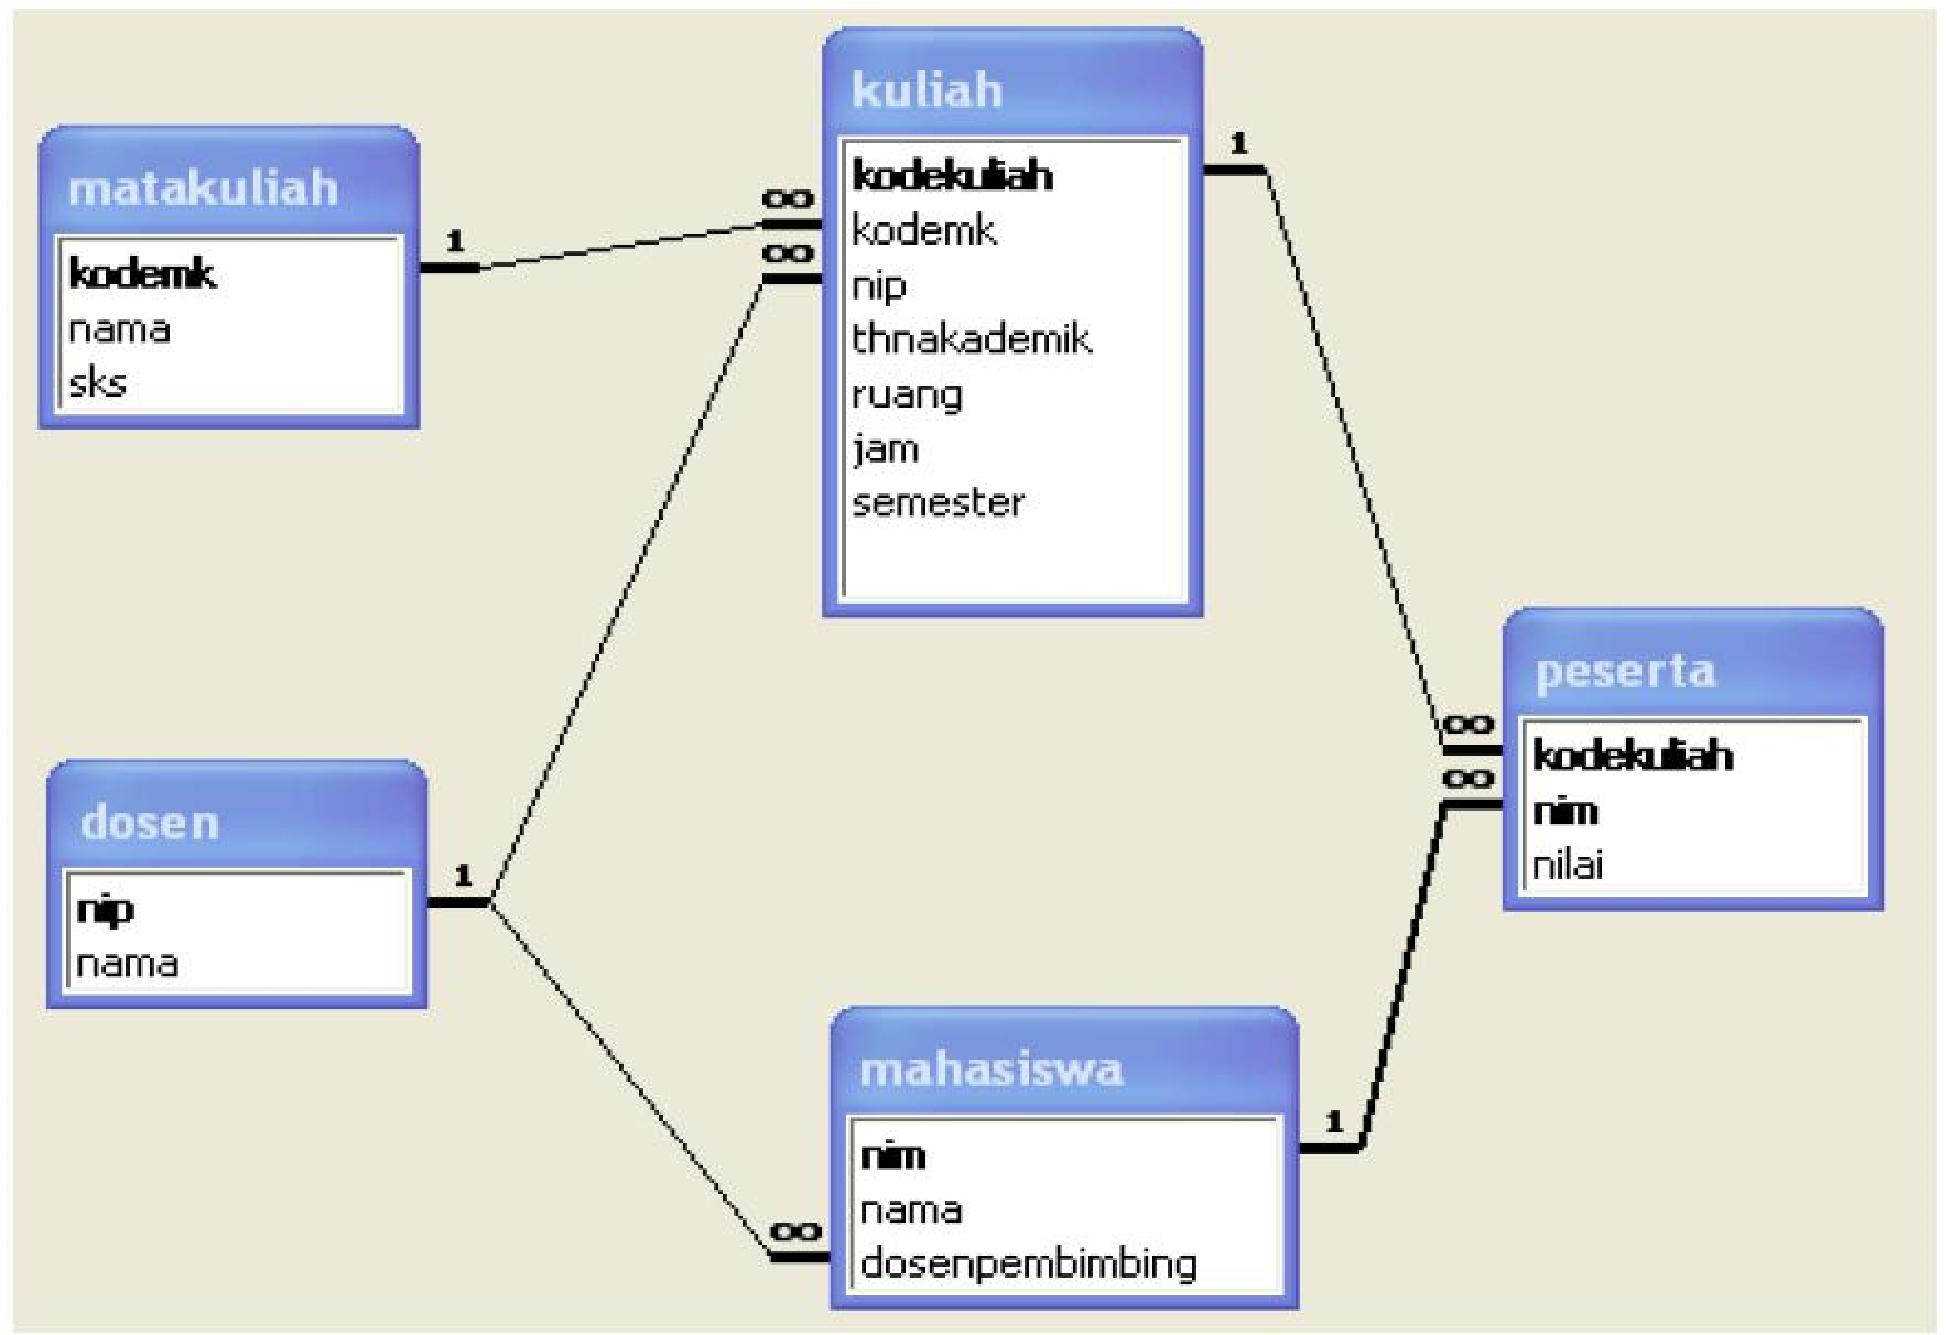
\includegraphics[width=0.7\linewidth]{images/basis-data-qt}
\caption{Pemrograman Basis data Qt Creator}
\label{fig:basis-data-qt}
\end{figure}


Pada contoh diatas, terdapat sebuah basisdata perkuliahan, dimana
terdapat 5 buah tabel. Tabel yang ada memiliki field (atribut/kolom).
Field pada masing-masing tabel sangat berasosiasi dengan tabelnya,
artinya kodemk, nama, dan sks pada tabel matkuliah sangat spesifik
menggambarkan tabel matakuliah, demikian juga yang lainnya.

Kita tidak akan membahas lebih lanjut tentang basisdata. Pada basis data
kita juga mengenal SQL (Structured Query Language). SQL merupakan bahasa
untuk mengakses dan memanipulasi basis data terutama isi record-record
pada tabel.

\subsection{Koneksi Qt dengan Basisdata}\label{koneksi-qt-dengan-basisdata}

Untuk melakukan koneksi pada basis data, Qt menyediakan dukungan pada
beberapa basis data yang terkenal, misalnya
\href{https://www.sqlite.org/about.html}{Sqlite},
\href{https://en.wikipedia.org/wiki/Oracle_Database}{Oracle},
\href{https://www.mysql.com/about/}{MySQL}, Db2\footnote{\href{https://en.wikipedia.org/wiki/IBM_DB2}{IBM
  DB2} adalah produk database server yang dikembangkan oleh IBM.
  Produk-produk ini mendukung sistem manajemen basis data relasional
  (relational DBMS), namun belakangan ini sudah mendukung pula sistem
  manajemen basis data berbasis object-relational (object-relational
  DBMS) dan juga non-relational seperti XML.}, ODBC\footnote{Open
  Database Connectivity (ODBC) adalah Application Programming interface
  (API) database yang khusus digunakan untuk mengakses database
  relasional. ODBC terdapat dalam setiap komputer yang menggunakan
  sistem operasi windows, karena ODBC merupakan bagian dari Windows Open
  System Architecture (WOSA). Dalam ODBC disediakan berbagai Application
  Programming Interface (API) yang berguna untuk menyediaan dan
  memberikan stkitar bagi berbagai kegiatan pemrograman. Keuntungan
  utama menggunakan ODBC ini adalah fleksibilitas, fleksibel disini
  artinya pengubahan jenis database yang dipergunakan oleh sebuah
  aplikasi tidak akan mempengaruhi kode program aplikasi tersebut.}, dan
\href{https://id.wikipedia.org/wiki/PostgreSQL}{Postgresql}. Secara
default basis data yang didukung adalah Sqlite dan ODBC saja, sedangkan
untuk basis data lainnya harus menggunakan driver yang biasanya harus
didownload pada situsnya secara langsung.

Pada Qt kita dapat membuat aplikasi console yang terkoneksi dengan basis
data. Koneksi terhadap kedua database tersebut tidak perlu melakukan
konfigurasi dan mendownload driver tertentu. Pada tulisan ini kita akan
menggunakan basis data Sqlite.

\subsection{Koneksi Qt dengan MySQL dan menampilkan
datanya}\label{koneksi-qt-dengan-mysql-dan-menampilkan-datanya}

\href{https://www.mysql.com/}{MySQL} merupakan database yang sudah
disupport oleh Qt. Untuk membuat database MySQL.

Untuk melakukan koneksi QtConsole dengan MySQL, maka lakukan Contoh
berikut:

\subsubsection*{Contoh Percobaan koneksi MySQL dengan QtConsole}

\begin{enumerate}


\item
  Buatlah sebuah database pada MySQL dengan nama: testmhs
\item
  Gunakan gunakan PHPmyAdmin untuk membuat tabel database.
  
  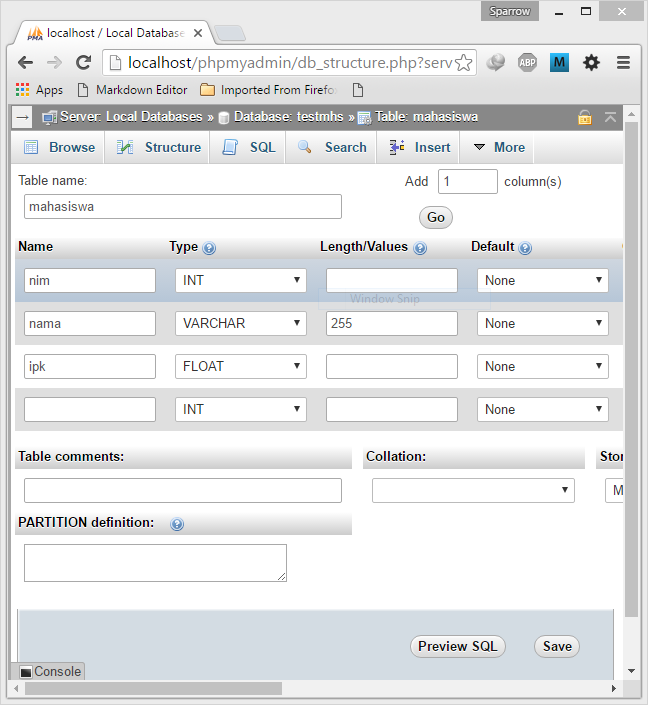
\includegraphics[width=0.7\linewidth]{images/phpmyadmin}
  
\item
  Isilah datanya sebagai berikut:

\begin{longtable}[]{@{}lll@{}}
\toprule
NIM & Nama & IPK\tabularnewline
\midrule
\endhead
011041 & Wachid & 3.6\tabularnewline
012042 & Arif & 3.6\tabularnewline
011012 & Eko & 3.4\tabularnewline
\bottomrule
\end{longtable}

Hasil:

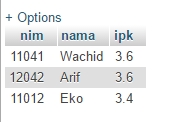
\includegraphics[width=0.7\linewidth]{images/database-mhs}

\item
  Tulis kode berikut ini:


\begin{lstlisting}[language=c++, caption=Percobaan koneksi MySQL dengan QtConsole]
#include <QtCore/QCoreApplication>
#include <QtSql/QtSql>
#include <QtDebug>
int main(int argc, char *argv[])
    {
QCoreApplication a(argc, argv);
qDebug() << QSqlDatabase::drivers();
QSqlDatabase db = QSqlDatabase::addDatabase("QMYSQL");
db.setDatabaseName( "testmhs" );
db.setHostName("localhost");
db.setUserName("root");
db.setPassword("");
if( !db.open() )
{
qDebug() << db.lastError();
qFatal( "Failed to connect." );
} else {
qDebug() << "Koneksi sukses";
QSqlQuery query(db);
query.exec("SELECT * FROM mahasiswa");
while (query.next()) {
qDebug() << query.value(0).toString();
qDebug() << query.value(1).toString();
qDebug() << query.value(2).toString();
}
}
return a.exec();
}
\end{lstlisting}

\item
  Pada file project yang berekstensi .pro, tambahkan linking ke library
  sql sebagai berikut:
  
  \begin{lstlisting}[language=c++]
#-------------------------------------------------
#
# Project created by QtCreator 2016-01-03T19:58:33
#
#-------------------------------------------------
QT += core
QT += gui
Qt += sql
TARGET = databases
CONFIG += console
CONFIG -= app_bundle
TEMPLATE = app
SOURCES += main.cpp
  \end{lstlisting}
\item
  Kemudian run dan hasilnya adalah sebagai berikut:

\begin{lcverbatim}
("QSQLITE", "QMYSQL", "QODBC3", "QODBC")
Koneksi sukses
"11041"
"Wachid"
"3.6"
"12042"
"Arif"
"3.6"
"11012"
"Eko"
"3.4"
\end{lcverbatim}
\end{enumerate}

\textbf{Keterangan:}

\begin{itemize}

\item
  Program diatas dapat menampilkan driver database yang terinstall dan
  dapat dikenali oleh system Qt, yaitu QSQLITE, QMYSQL, QODBC3, dan
  QODBC. Berarti sistem QT dapat mendukung basisdata Sqlite, MySQL, dan
  ODBC dari Microsoft.
\item
  Kemudian langkah pertama yang harus dilakukan adalah membuat
  QsqlDatabase yang akan meload basis data yang dipilih beserta dengan
  drivernya. Setelah itu kita harus menentukan nama database yang akan
  diakses, user, password, dan host lokasi MySQL server.
\item
  Kemudian akan diperiksa apakah database yang terpilih dapat dibuka
  atau tidak dengan method open(). Jika berhasil maka akan dilanjutkan,
  jika tidak maka akan ditampilkan error yang terjadi dengan menggunakan
  method dari database, yaitu lastError().
\item
  Langkah berikutnya adalah melakukan query dengan menggunakan method
  query(). Setelah perintah SQL dijalankan maka record-record yang
  dihasilkan dari perintah select tersebut akan diloop satu persatu
  dengan method next() dari query, dan ditampilkan hasilnya dilayar.
\end{itemize}

\subsection{Koneksi Qt dengan SQLite}\label{koneksi-qt-dengan-sqlite}

SQLite merupakan database yang sudah disupport secara native oleh Qt.
Untuk membuat database SQLite, kita membutuhkan tool yang dapat
digunakan untuk mengelola databasenya dengan mudah, silahkan gunakan
sqliteadmin\footnote{http://www.sqliteexpert.com/} yang berbasis desktop.

Yang perlu diperhatikan ketika kita membuat koneksi dengan basisdata
SQLite adalah:

\begin{enumerate}


\item
  Jika basis data SQLite akan dibuat langsung dari program, maka file
  database hasil pembuatan tersebut akan berada di folder simulator pada
  project kita.
\item
  Jika kita sudah memiliki file database SQLite, maka file tersebut
  harus diletakkan (dikopikan) ke folder simulator atau simulator \textfractionsolidus debug
\item
  File SQLite yang dibuat harus berjenis SQLite 3 agar bisa diakses.
\end{enumerate}

Untuk melakukan koneksi QtConsole dengan SQLite, maka lakukan Contoh
berikut:

\subsubsection*{Contoh Percobaan koneksi SQLite dengan QtConsole}

\begin{enumerate}


\item
  Buatlah sebuah database pada Sqlite dengan nama: testmhs.db, ingat
  harus berjenis SQLite3.

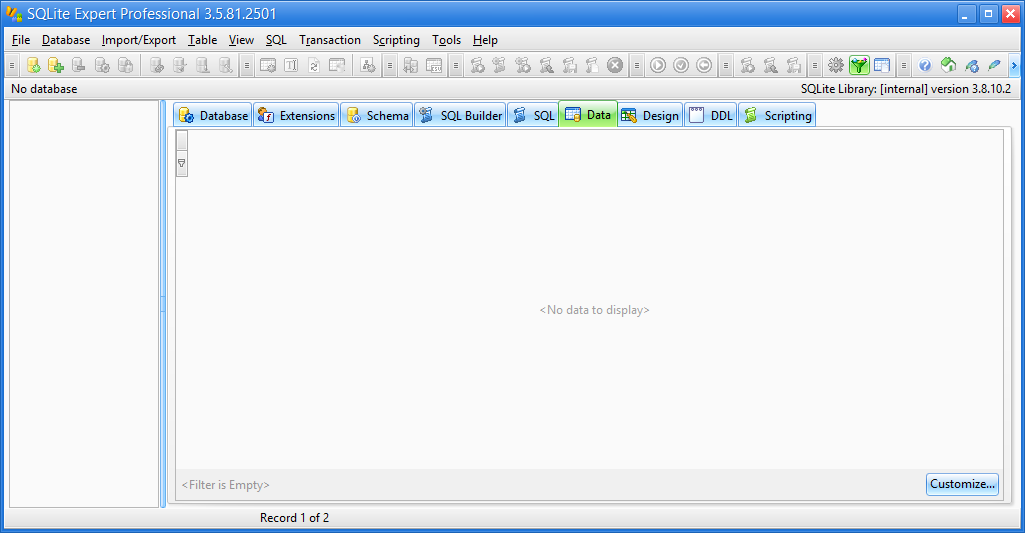
\includegraphics[width=0.7\linewidth]{images/sqlite-expert}
  
  
\item
  Gunakan Sqlite Expert untuk membuatnya
\item
  Pilih menu File \textgreater{} New Database
  
  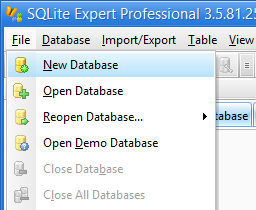
\includegraphics[width=0.7\linewidth]{images/file-new-database}
  
\item
  Simpan dengan nama testmhs.db (pilih tipe sqlite 3 database), simpan
  pada folder project yang akan dibuat.
\item
  Kemudian buat tabel baru dengan klik menu table \textgreater{} New Table,
  kemudian isikan data berikut:

Nama tabel: mahasiswa

Field:

\begin{itemize}

\item
  NIM tipe VARCHAR(8), primary key, not null, unique
\item
  Nama tipe VARCHAR(30), not null
\item
  IPK tipe FLOAT
\end{itemize}


\item
  Kemudian isi data sebagai berikut:


\begin{longtable}[]{@{}lll@{}}
\toprule
NIM & Nama & IPK\tabularnewline
\midrule
\endhead
011041 & Wachid & 3.6\tabularnewline
012042 & Arif & 3.6\tabularnewline
011012 & Eko & 3.4\tabularnewline
\bottomrule
\end{longtable}


\item
  Setelah itu buatlah project baru pada QtConsole application, dan
  tulislah kode program berikut:

\begin{lstlisting}[language=c++, caption=Percobaan koneksi SQLite dengan QtConsole]
#include <QtCore/QCoreApplication>
#include <QDebug>
#include <QtSql/QtSql>
    int main(int argc, char *argv[])
{
QCoreApplication a(argc, argv);
qDebug() << QSqlDatabase::drivers();
QSqlDatabase db = QSqlDatabase::addDatabase("QSQLITE");
db.setDatabaseName( "testmhs.db" );
if( !db.open() )
{
qDebug() << db.lastError();
qFatal( "Failed to connect." );
} else qDebug() << "Koneksi berhasil";
return a.exec();
}
\end{lstlisting}

\item
  Pada project, pilihlah file berekstensi .pro, kemudian bukalah file
  tersebut dan tambahkanlah bagian kode berikut:
  
  \begin{lstlisting}[language=c++]
  #-------------------------------------------------
  #
  # Project created by QtCreator 2016-01-03T19:58:33
  #
  #-------------------------------------------------
  QT += core
  QT += gui
  Qt += sql
  TARGET = databases
  CONFIG += console
  CONFIG -= app_bundle
  TEMPLATE = app
  SOURCES += main.cpp
  \end{lstlisting}
  
\item
  Build dan run

\begin{lcverbatim}
("QSQLITE")
Koneksi berhasil
\end{lcverbatim}
\end{enumerate}

\textbf{Keterangan:}

\begin{itemize}

\item
  Baris pertama output adalah daftar driver yang didukung oleh Qt dan
  QtCreator.
\item
  Baris kedua adalah menggambarkan bahwa koneksi terhadap database
  Sqlite berhasil!
\item
  Program diatas mengharuskan adanya urutan perintah yang harus
  dilakukan ketika kita akan melakukan koneksi ke database Sqlite,
  yaitu: 

\begin{itemize}
\item Load driver SQLITE Tambahkan bagian ini
\item setDatabaseName sesuai dengan nama file Sqlite yang akan diakses 
\item Kemudian open koneksi dengan memanggil method open 
\item Jika ada error tampilkan errornya, jika tidak tampilkan bahwa koneksi berhasil
\end{itemize}  

\end{itemize}

\subsection{Membaca data pada tabel SQLITE}

Cara membaca data pada tabel Sqlite adalah dengan menggunakan perintah
query SQL SELECT. Sintaksnya adalah
\texttt{SELECT\ \textless{}field,\ field,\ field\textgreater{}\ FROM\ \textless{}nama\_tabel\textgreater{}\ WHERE\ \textless{}kondisi\textgreater{}}
Perintah diatas bisa menghasilkan record atau malah salah sekali tidak
menghasilkan record apapun. Jika menghasilkan record, maka record yang
dihasilkan bisa satu atau lebih dari satu.

Pada Qt cara yang digunakan untuk membaca data adalah dengan menggunakan
class QSqlQuery dan method query seperti berikut ini:

\begin{lstlisting}[language=c++, numbers=none]
QSqlQuery query("SELECT * FROM mahasiswa");
while (query.next()) {
QString nim = query.value(0).toString();
qDebug() << nim;
}
\end{lstlisting}

Kita ingat bahwa tabel mahasiswa memiliki 3 kolom: NIM, Nama, dan IPK.

Perintah diatas menggunakan QsqlQuery yang menerima parameter Qstring.
Setelah query dijalankan maka akan dilakukan proses looping untuk
mengambil data-data per baris record dengan menggunakan method next()
dari query. Di dalam looping kita mengambil variabel nim pada kolom
pertama (dalam hal ini digunakan indeks 0). Untuk mengambil field
tertentu pada tabel, misalnya ipk, maka hanya perlu mengganti indeksnya
menjadi 2 saja.

\subsubsection*{Contoh  Membaca data pada Sqlite.}

Tulislah program berikut:

\begin{lstlisting}[language=c++, caption= Membaca data pada Sqlite]
#include <QtCore/QCoreApplication>
#include <QDebug>
#include <QtSql/QtSql>
int main(int argc, char *argv[])
{
QCoreApplication a(argc, argv);
qDebug() << QSqlDatabase::drivers();
QSqlDatabase db = QSqlDatabase::addDatabase("QSQLITE");
db.setDatabaseName("testmhs.db");
if(!db.open())
{
qDebug() << db.lastError();
qFatal( "Failed to connect." );
} else qDebug() << "Koneksi berhasil";
    QSqlQuery query;
bool cek = query.exec("select nim,nama from mahasiswa order by nim desc");
qDebug() << cek;
QString nim,nama;
while(query.next())
{
nim = query.value(0).toString();
nama = query.value(1).toString();
qDebug() << nim << " " << nama;
}
return a.exec();
}
\end{lstlisting}

\textbf{Hasil:}

\begin{lcverbatim}
("QSQLITE")
Koneksi berhasil
true
"11041""Wachid"
"12042""Arif"
"11012""Eko"
\end{lcverbatim}

\textbf{Keterangan:}

\begin{itemize}

\item
  Program diatas melakukan koneksi ke SQLite dan kemudian mengirimkan
  query untuk mengambil data-data dari tabel mahasiswa dengan
  menggunakan query SQL select.
\item
  Untuk mendapatkan hasil dari query kita gunakan perulangan dari
  variabel query dan method next(). Didalam perulangan kita ambil
  masing-masing nilai dari tiap-tiap kolom untuk setiap recordnya dengan
  menggunakan query.value().toString()
\item
  Perintah diatas berarti kita mengambil indeks sesuai dengan kolom yang
  diambil dari SQL, yaitu kolom 0 untuk nim, 1 untuk nama dan
  seterusnya.
\end{itemize}

\subsection{Menambah data pada tabel SQLITE}\label{menambah-data-pada-tabel-sqlite}

Cara menambah data pada tabel Sqlite adalah dengan menggunakan perintah
query SQL INSERT. Sintaksnya adalah
\texttt{INSERT\ INTO\ \textless{}namatabel\textgreater{}\ (\textless{}kolom1\textgreater{},\textless{}kolom2\textgreater{},\ dst)\ VALUES\ (\textless{}nilai1\textgreater{},\ \textless{}nilai2\textgreater{}},
dst) Perintah diatas tidak menghasilkan record sama sekali, namun dapat
menghasilkan berapa jumlah record yang terpengaruh (affected rows) dan
juga mengembalikan nilai bool yang akan bernilai true atau false. Nilai
true jika menambahan data berhasil, nilai false jika penambahan data
gagal.

Pada Qt cara yang digunakan untuk menambah data adalah dengan
menggunakan class QSqlQuery dan method query seperti berikut ini:

\begin{lstlisting}[language=c++, numbers=none]
QSqlQuery query;
bool hasil = query.exec("INSERT INTO mahasiswa (nim, nama,ipk) VALUES
('22113344','anton', 3.4)");
if(hasil) qDebug() << "Berhasil"; else qDebug << "gagal";
\end{lstlisting}

Perintah diatas menggunakan QsqlQuery yang menerima parameter sql dalam
tipe data Qstring. Setelah query dijalankan maka akan diperiksa hasil
dari akibat penambahan datanya. Jika berhasil maka akan mengembalikan
nilai true, sedangkan jika gagal maka akan menghasilkan nilai false.

\subsubsection*{Contoh  Menambahkan data pada SQLite.}

Buatlah program berikut:

\begin{lstlisting}[language=c++, caption= Menambahkan data pada SQLite]
#include <QtCore/QCoreApplication>
#include <QDebug>
#include <QtSql/QtSql>
int main(int argc, char *argv[])
{
QCoreApplication a(argc, argv);
qDebug() << QSqlDatabase::drivers();
QSqlDatabase db = QSqlDatabase::addDatabase("QSQLITE");
db.setDatabaseName("testmhs.db");
if(!db.open())
{
qDebug() << db.lastError();
qFatal( "Failed to connect." );
} else qDebug() << "Koneksi berhasil";
QSqlQuery query;
bool hasil = query.exec("insert into mahasiswa(nim,nama,ipk) values
('22334455','mhs baru',3.12)");
if(hasil) qDebug() << "Berhasil ditambahkan"; else qDebug() << "Gagal
ditambahkan";
return a.exec();
}
\end{lstlisting}

\textbf{Hasil:}

\begin{lcverbatim}
("QSLITE")
Koneksi berhasil
Berhasil ditambahkan
\end{lcverbatim}

\textbf{Keterangan:}

\begin{itemize}
\item
  Pada awalnya data pada tabel mahasiswa hanya berjumlah 3 buah data,
  ketika program dijalankan maka data baru bernama ``mhs baru'' berhasil
  ditambahkan dan mengubah jumlah record pada tabel sehingga menjadi 4
  buah. Tampilan perubahan adalah sebagai berikut:
  
  \begin{tabular}{|l|l|l|}
  \hline
  NIM & Nama & IPK \\ \hline
  011041 & Wachid & 3.1 \\ \hline
  012042 & Arif & 3.6 \\ \hline
  011041 & Eko & 3.4 \\ \hline
  012011 & Alif & 3.3 \\ \hline
  013021 & Ananda & 3.8 \\ \hline
  
  \end{tabular}
\item
  Cara menambahkan record pada SQLite sangat mudah, yaitu dengan
  menggunakan SQL insert into yang harus disesuaikan dengan jumlah field
  yang ada pada tabel. Setelah itu query akan dijalankan dengan method
  exec dari obyek QsqlQuery.
\item
  Hasil kembalian dari method exec ini adalah bool yang menghasilkan
  nilai true atau false. Jika menghasilkan nilai true maka record
  berhasil ditambahkan, jika false maka record tidak berhasil
  ditambahkan!
\item
  Jika program diatas dieksekusi sekali lagi (diulangi) maka akan
  menampilkan tulisan Gagal ditambahkan. Hal ini dikarenakan kita
  menambahkan record yang sama persis dengan ebelumnya padahal kita
  sudah menset bahwa field nim bersifat primary, yang artinya tidak
  boleh ada data nim yang kembar. Hal inilah yang menyebabkan data Gagal
  ditambahkan.
  \begin{lcverbatim}
  ("QSLITE")
  Koneksi berhasil
  gagal  ditambahkan
\end{lcverbatim}

\item Jika kita hendak membaca data pada SQLite, maka tambahkan kode berikut:

\begin{lstlisting}[language=c++, caption=Membaca data pada SQLite]
QsqlQuery query.exec("select nim,nama,ipk from mahasiswa order by nim desc");
QString nim,nama;
float ipk;
while(query.next())
{
nim = query.value(0).toString();
nama = query.value(1).toString();
ipk = query.value(2).toFloat();
qDebug() << nim << " " << nama << " " << ipk;
}
\end{lstlisting}

\item Sehingga akan dihasilkan:

\begin{lcverbatim}
"012011"  "Alif"  "3.3"
"013021"  "Ananda"  "3.8" 
"011041" "Wachid"  "3.1" 
"012042"  "Arif"  "3.6" 
"011012"  "Eko"  "3.4" 

\end{lcverbatim}
\end{itemize}



\subsection{Mengedit data pada tabel SQLITE}\label{mengedit-data-pada-tabel-sqlite}

Cara mengedit data pada tabel Sqlite adalah dengan menggunakan perintah
query SQL UPDATE. Sintaksnya adalah
\texttt{UPDATE\ \textless{}namatabel\textgreater{}\ SET\ \textless{}kolom1\textgreater{}=\textless{}nilaikolom1\textgreater{},\textless{}kolom2\textgreater{}=\textless{}nilaikolom2\textgreater{}},
dst \texttt{WHERE\ \textless{}kriteri} Perintah diatas tidak
menghasilkan record sama sekali, namun dapat menghasilkan berapa jumlah
record yang terpengaruh (affected rows) dan juga mengembalikan nilai
bool yang akan bernilai true atau false. Nilai true jika pengeditan data
berhasil, nilai false jika pengeditan data gagal.

Pada Qt cara yang digunakan untuk mengedit data adalah dengan
menggunakan class QSqlQuery dan method query seperti berikut ini:

\begin{lstlisting}[language=c++, caption=menggunakan class QSqlQuery dan method query]
QSqlQuery query;
bool hasil = query.exec("UPDATE mahasiswa SET nama='Antonius Rachmat C' WHERE
nim='2200259');
if(hasil) qDebug() << "Berhasil"; else qDebug << "gagal";
\end{lstlisting}

Perintah diatas menggunakan QsqlQuery yang menerima parameter sql dalam
tipe data Qstring. Setelah query dijalankan maka akan diperiksa hasil
dari akibat pengeditan datanya. Jika berhasil maka akan mengembalikan
nilai true, sedangkan jika gagal maka akan menghasilkan nilai false.

\subsubsection*{Contoh Mengedit data pada SQLite.}

\begin{enumerate}
\item Kondisi awal tabel:

\begin{tabular}{|l|l|l|}
\hline
NIM & Nama & IPK \\ \hline
011041 & Wachid & 3.1 \\ \hline
012042 & Arif & 3.6 \\ \hline
011041 & Eko & 3.4 \\ \hline
012011 & Alif & 3.3 \\ \hline
013021 & \colorbox{red}{Ananda} & 3.8 \\ \hline
\end{tabular}

Kita akan mengedit nim 013021 menjadi bernama Aryo

\item Buatlah program berikut:

\begin{lstlisting}[language=c++, caption=Mengedit data pada SQLite]
#include <QtCore/QCoreApplication>
#include <QDebug>
#include <QtSql/QtSql>
#include <iostream>
using namespace std;
int main(int argc, char *argv[])
{
QCoreApplication a(argc, argv);
qDebug() << QSqlDatabase::drivers();
QSqlDatabase db = QSqlDatabase::addDatabase("QSQLITE");
db.setDatabaseName("testmhs.db");
if(!db.open())
{
qDebug() << db.lastError();
qFatal( "Failed to connect." );
} else qDebug() << "Koneksi berhasil";
QSqlQuery query;
bool hasil = query.exec("update mahasiswa set nama='Antonius Rachmat C' where
nim='22002529'");
if(hasil) qDebug() << "Berhasil diedit"; else qDebug() << "Gagal diedit";
qDebug() << "Jumlah record yang diedit: " << query.numRowsAffected();
return a.exec();
}
\end{lstlisting}

\item \textbf{Hasil:}
\begin{lcverbatim}
("QSLITE")
Koneksi berhasil
Berhasil diedit
Jumlah record yang diedit : 1
\end{lcverbatim}
\item Kondisi akhir tabel:

\begin{tabular}{|l|l|l|}
\hline
013021 & Ananda & 3.8 \\ \hline
NIM & Nama & IPK \\ \hline
011041 & Wachid & 3.1 \\ \hline
012042 & Arif & 3.6 \\ \hline
011041 & Eko & 3.4 \\ \hline
012011 & Alif & 3.3 \\ \hline

\end{tabular}
\end{enumerate}

\textbf{Keterangan:}

\begin{itemize}

\item
  Program diatas masih sama menggunakan obyek QsqlQuery dan method
  exec(). Hanya SQL query nya saja yang berbeda dengan Contoh sebelumnya
  saat penambahan data. SQL query pada saat pengeditan menggunakan SQL
  UPDATE SET.
\item
  Untuk mengetahui berapa jumlah record yang terupdate digunakan method
  numRowsAffected() dari obyek QsqlQuery.
\end{itemize}

\subsection{Menghapus data pada tabel SQLITE}\label{menghapus-data-pada-tabel-sqlite}

Cara menghapus data pada tabel Sqlite adalah dengan menggunakan perintah
query SQL UPDATE. Sintaksnya adalah DELETE FROM WHERE \textless{}kriteri
Perintah diatas tidak menghasilkan record sama sekali, namun dapat
menghasilkan berapa jumlah record yang terpengaruh (affected rows) dan
juga mengembalikan nilai bool yang akan bernilai true atau false. Nilai
true jika penghapusan data berhasil, nilai false jika penghapusan data
gagal.

Pada Qt cara yang digunakan untuk menghapus data adalah dengan
menggunakan class QSqlQuery dan method query seperti berikut ini:

\begin{lstlisting}[language=c++, caption=menghapus data adalah dengan menggunakan class QSqlQuery dan method query]
QSqlQuery query;
bool hasil = query.exec("DELETE FROM mahasiswa WHERE nim='22334455');
if(hasil) qDebug() << "Berhasil"; else qDebug << "gagal";
\end{lstlisting}

Perintah diatas menggunakan QsqlQuery yang menerima parameter sql dalam
tipe data Qstring. Setelah query dijalankan maka akan diperiksa hasil
dari akibat penghapusan datanya. Jika berhasil maka akan mengembalikan
nilai true, sedangkan jika gagal maka akan menghasilkan nilai false.

\subsubsection*{Contoh  Menghapus data pada SQLite.}

\begin{enumerate}
\item Kondisi awal tabel:

\begin{tabular}{|l|l|l|}
\hline
NIM & Nama & IPK \\ \hline
011041 & Wachid & 3.1 \\ \hline
012042 & Arif & 3.6 \\ \hline
011041 & Eko & 3.4 \\ \hline
012011 & Alif & 3.3 \\ \hline
013021 & \colorbox{red}{Ananda} & 3.8 \\ \hline
\end{tabular}

Kita akan menghapus data ``Ananda''.

\item Buatlah program sebagai berikut:

\begin{lstlisting}[language=c++, caption= Menghapus data pada SQLite]
#include <QtCore/QCoreApplication>
#include <QDebug>
#include <QtSql/QtSql>
#include <iostream>
using namespace std;
int main(int argc, char *argv[])
{
QCoreApplication a(argc, argv);
qDebug() << QSqlDatabase::drivers();
QSqlDatabase db = QSqlDatabase::addDatabase("QSQLITE");
db.setDatabaseName("testmhs.db");
if(!db.open())
{
qDebug() << db.lastError();
qFatal( "Failed to connect." );
} else qDebug() << "Koneksi berhasil";
QSqlQuery query;
bool hasil = query.exec("delete from mahasiswa where nim='22334455'");
if(hasil) qDebug() << "Berhasil dihapus"; else qDebug() << "Gagal dihapus";
qDebug() << "Jumlah record yang dihapus: " << query.numRowsAffected();
return a.exec();
}
\end{lstlisting}

\item \textbf{Hasil:}

\begin{lcverbatim}
("QSLITE")
Koneksi berhasil
Berhasil diedit
Jumlah record yang dihapus : 1
\end{lcverbatim}

\item Kondisi akhir tabel:

\begin{tabular}{|l|l|l|}
\hline
NIM & Nama & IPK \\ \hline
011041 & Wachid & 3.1 \\ \hline
012042 & Arif & 3.6 \\ \hline
011041 & Eko & 3.4 \\ \hline
012011 & Alif & 3.3 \\ \hline

\end{tabular}

\end{enumerate}

\textbf{Keterangan:}

Program diatas mampu menghapus data pada suatu record tertentu dengan
menggunakan perintah SQL DELETE FROM. Program diatas tidak ada perubahan
dari Contoh sebelumnya kecuali bagian perintah SQL nya.

Demikianlah kita sudah berlatih sejumlah manipulasi data pada tabel
SQLite dengan menggunakan QtSql. Pada databse lain misalnya MySQL semua
perintah --perintah yang sudah dipelajari dapat digunakan dan hanya
perlu disesuaikan pada bagian koneksi pada databasenya. Pemrograman
basis data pada Qt termasuk mudah.

Pada bagian berikutnya kita akan mencoba membuat program untuk
memanipulasi data pada tabel mahasiswa dengan menggunakan menu. Pada
menu akan ditampilkan beberapa pilihan seperti:

\begin{enumerate}


\item
  Tambah data
\item
  Tampil data
\item
  Hapus data
\item
  Cari nim
\item
  Edit data
\item
  Exit
\end{enumerate}

Penjelasan:

\begin{itemize}

\item
  Menu 1 akan digunakan untuk menambah data mahasiswa
\item
  Menu 2 akan digunakan untuk menampilkan data semua mahasiswa
\item
  Menu 3 akan digunakan untuk menghapus data seorang mahasiswa
  berdasarkan nimnya
\item
  Menu 4 akan digunakan untuk mencari data seorang mahasiswa berdasarkan
  nimnya
\item
  Menu 5 akan digunakan untuk mengedit data seorang mahasiswa
  berdasarkan nimnya
\end{itemize}

Cara yang digunakan adalah dengan membuat sebuah class yang akan
digunakan untuk mengakses semua fungsi yang berhubungan dengan
manipulasi data pada basis data SQLite. Method pada class adalah connect
untuk koneksi database, sebuah konstruktor dan method untuk mengambil
nama tabel serta nama database SQLitenya. Kemudian akan dibuat
fungsi-fungsi lain diluar class yang digunakan untuk melakukan
fungsi-fungsi sesuai dengan 5 fungsi yang didefinisikan pada menu. Untuk
lebih jelasnya silahkan dicoba pada Contoh berikut ini.

\subsubsection*{Contoh  Pembuatan manipulasi data pada SQLite dengan menggunakan menu}

\begin{enumerate}

\item
  Tulislah program berikut:

\begin{lstlisting}[language=c++, caption= Pembuatan manipulasi data pada SQLite dengan menggunakan menu]
#include <QtCore/QCoreApplication>
#include <QDebug>
#include <QtSql/QtSql>
#include <iostream>
#include <conio.h>
using namespace std;
class Tabel{
private:
QString namadb;
QString namatabel;
QString strquery;
QSqlDatabase db;
public:
//konstruktor
Tabel(QString namadb, QString namatabel){
this->namadb = namadb;
this->namatabel = namatabel;
}
bool connect(){
this->db = QSqlDatabase::addDatabase("QSQLITE");
this->db.setDatabaseName(this->namadb);
if(!this->db.open())
{
qDebug() << "No";
return false;
} else {
qDebug() << "Yes";
return true;
}
}
bool jalanQuery(QString query){
this->strquery = query;
bool hasil = false;
if(this->db.isOpen()){
QSqlQuery myq(this->db);
hasil = myq.exec(this->strquery);
}
return hasil;
}
void ambilData(QString query){
this->strquery = query;
if(this->db.isOpen()){
QSqlQuery myq(this->db);
myq.exec(this->strquery);
QSqlRecord rec = myq.record();
int cols = rec.count();
QString temp;
for( int c=0; c<cols; c++ )
temp += rec.fieldName(c) + ((c<cols-1)?"\t":"");
qDebug() << temp;
while( myq.next() )
{
temp = "";
for( int c=0; c<cols; c++ )
temp += myq.value(c).toString() + ((c<cols-1)?"\t":"");
qDebug() << temp;
}
    }
}
QString getNamaTabel(){
return this->namatabel;
}
QString getNamaDb(){
return this->namadb;
}
QSqlDatabase getDb(){
return this->db;
}
};
void tambahData(Tabel t){
string nim,nama,ipk;
getline(cin,nim);
cout << "NIM: "; getline(cin,nim);
cout << "Nama: "; getline(cin,nama);
cout << "IPK: "; getline(cin,ipk);
QString s = "insert into "+t.getNamaTabel()+" values
('"+nim.c_str()+"','"+nama.c_str()+"',"+ipk.c_str()+")";
bool hasil = t.jalanQuery(s);
if(hasil) qDebug() << "Penambahan berhasil"; else qDebug() << "Penambahan gagal";
}
void hapusData(Tabel t){
string nim;
getline(cin,nim);
cout << "NIM yang akan dihapus: "; getline(cin,nim);
QString s = "delete from "+t.getNamaTabel()+" where nim='"+nim.c_str()+"'";
bool hasil = t.jalanQuery(s);
if(hasil) qDebug() << "Penghapusan berhasil"; else qDebug() << "Penghapusan
gagal";
}
void tampilData(Tabel t){
QString s = "select * from "+t.getNamaTabel()+" order by nim asc";
t.ambilData(s);
}
void cariNim(Tabel t){
string nim;
getline(cin,nim);
cout << "NIM yang akan dicari: "; getline(cin,nim);
QString s = "select * from "+t.getNamaTabel()+" where nim='"+nim.c_str()+"'";
t.ambilData(s);
}
void editData(Tabel t){
string nim,nama,ipk;
getline(cin,nim);
cout << "NIM yang akan diedit: "; getline(cin,nim);
cout << "Nama baru: "; getline(cin,nama);
cout << "IPK baru: "; getline(cin,ipk);
QString s = "update "+t.getNamaTabel()+" set
nama='"+nama.c_str()+"',ipk="+ipk.c_str()+" where nim='"+nim.c_str()+"'";
bool hasil = t.jalanQuery(s);
if(hasil) qDebug() << "Pengeditan berhasil"; else qDebug() << "Pengeditan gagal";
}
    int main(int argc, char *argv[])
{
QCoreApplication a(argc, argv);
int pil;
Tabel t("testmhs.db","mahasiswa");
t.connect();
do {
system("cls");
cout << "MENU" <<endl;
cout << "1. Tambah data\n";
cout << "2. Tampil data\n";
cout << "3. Hapus data\n";
cout << "4. Cari nim\n";
cout << "5. Edit data\n";
cout << "6. Exit\n";
cout << "Pilihan : "; cin >> pil;
cout << endl;
switch (pil) {
case 1:
tambahData(t);break;
case 2:
tampilData(t);break;
case 3:
hapusData(t);break;
case 4:
cariNim(t);break;
case 5:
editData(t);
}
cout << "Tekan sembarang tombol..."; getch();
} while (pil >=1 && pil<=5);
cout << "Good bye";
return a.exec();
}
\end{lstlisting}
\end{enumerate}

\textbf{Hasil:}

\begin{enumerate}

\item
  Tampilan menu:
  
 \begin{lcverbatim}
MENU:
1. Tambah data
2. Tampil data
3. Hapus data
4. Cari nim
5. Edit data
6. Exit
Pilihan:
 \end{lcverbatim}

\item
  Menu tambah data dan tampil data:
  
 \begin{lcverbatim}
 MENU:
 1. Tambah data
 2. Tampil data
 3. Hapus data
 4. Cari nim
 5. Edit data
 6. Exit
 Pilihan: 1
 NIM: 013012
 Nama: Ramadhani
 Penambahan berhasil
 Tekan sembarang tombol . . .
 \end{lcverbatim}
  
\begin{lcverbatim}
"NIM  Nama  IPK" 
"011041  Wachid  3.1" 
"012042  Arif  3.6 "
"011041  Eko  3.4"
"012011  Alif  3.3" 
"013012 Ramadhani   3.8" 
  \end{lcverbatim}
\item
  Menu hapus data dan tampil data:
  
 \begin{lcverbatim}
MENU:
1. Tambah data
2. Tampil data
3. Hapus data
4. Cari nim
5. Edit data
6. Exit
Pilihan: 3
NIM yang akan dihapus: 011041
Penghapusan berhasil
Tekan sembarang tombol . . .
\end{lcverbatim}
\begin{lcverbatim}
"NIM  Nama  IPK" 
"012042  Arif  3.6 "
"011041  Eko  3.4"
"012011  Alif  3.3" 
"013012 Ramadhani   3.8" 
\end{lcverbatim}
   
\item
  Menu edit data dan tampil data: 
  
  Mengedit 011041 menjadi bernama
  Nur Wachid dan IPK menjadi 3.01
  
  \begin{lcverbatim}
  MENU:
  1. Tambah data
  2. Tampil data
  3. Hapus data
  4. Cari nim
  5. Edit data
  6. Exit
  Pilihan: 5
  NIM yang akan diedit: 011042
  Nama baru: Arif H
  IPK: 3.01
  Tekan sembarang tombol . . .
  \end{lcverbatim}
  
\begin{lcverbatim}
"NIM  Nama  IPK" 
"012042  Arif H  3.6 "
"011041  Eko  3.4"
"012011  Alif  3.3" 
"013012 Ramadhani   3.8" 
\end{lcverbatim}
\item
  Menu cari data:

\begin{lcverbatim}
MENU:
1. Tambah data
2. Tampil data
3. Hapus data
4. Cari nim
5. Edit data
6. Exit
Pilihan: 4
NIM yang akan dicari: 011042
"NIM  Nama  IPK" 
"012042  Arif H  3.6 "
Tekan sembarang tombol . . .
\end{lcverbatim}
\item
  Menu Exit

\begin{lcverbatim}
MENU:
1. Tambah data
2. Tampil data
3. Hapus data
4. Cari nim
5. Edit data
6. Exit
Pilihan: 6
Tekan sembarang tombol . . .Good bye
\end{lcverbatim}

\end{enumerate}

\textbf{Keterangan:}

\begin{itemize}

\item
  Program diatas merupakan program yang cukup banyak dan kompleks.
  Program ini dibuat dengan prinsip perulangan. Kita akan mengulang
  terus menerus bagian menu 1-6 sampai pengguna menginputkan angka yang
  bukan diantara 1-5. Jika pengguna memasukkan angka 1 maka dipanggil
  menu pertama, dan seterusnya. Jika pengguna memasukkan angka 6 maka
  program akan menampilkan Good Bye.
\item
  Pada awal program kita membuat sebuah class bernama Tabel yang
  digunakan untuk mengelola data-data pada tabel mahasiswa. Class Tabel
  harus diinisialisasi terlebih dahulu pada method int main() dengan
  mengiputkan nama database dan nama tabelnya. Setelah diinisialisai
  maka class Tabel harus melakukan method connect agar database SQLite
  terbuka (open).
\item
  Ketika menu penambahan data dipilih, maka method tambahData akan
  dipanggil dan membutuhkan parameter Tabel yang sudah dibuat dan
  diinisialisasi terlebih dahulu sebelumnya. Setelah itu berdasarkan
  obyek Tabel yang sudah dibuat, kita akan menggunakannya untuk
  memasukkan data.
\item
  Pada menu tambah, program akan meminta inputan nim, nama, dan ipk
  kepada pengguna. Setelah pengguna mengiputkan data dengan lengkap,
  maka method tambahData() akan dipanggil sehingga data dapat masuk ke
  tabel. Proses memasukkan data dilakukan dengan menggunakan query
  INSERT.
\item
  Demikian pula dengan menu tampil data, method yang digunakan sama pada
  contoh-contoh sebelumnya, namun ditambah dengan cara membaca
  kolom-kolom pada tabel dan menampilkan semua recordnya satu persatu
  dengan perulangan.
\item
  Pada menu hapus data, perintah yang digunakan juga hanya mengubah
  query SQLnya.
\item
  Pada menu cari data, kita juga menggunakan SQL select seperti pada
  menampilkan data. Perbedaannya hanyalah kondisi where yang digunakan.
  Pada menu pencarian data, kita mencari satu buah record mahasiswa saja
  berdasarkan nimnya.
\item
  Pada menu edit data, kita juga menggunakan SQL update yang dapat
  digunakan untuk mengubah data pada tabel. Pada menu edit ini, kita
  mencari terlebih dahulu nim mahasiswa yang akan diedit baru
  mengeditnya.
\end{itemize}

\begin{quotation}


\includegraphics{images/tips}\textbf{TIPS:} 

Untuk
mengkonversi dari tipe data string menuju ke Qstring, digunakan
\texttt{\textless{}variabel\ string\ bias.c\_str()} Perintah cin tidak
bisa digunakan setelah fungsi getline, karena akan membuat inputan
menjadi bertumpuk seperti pada contoh ini:

\begin{lstlisting}[language=c++, numbers=none]
int main(){
int id, age;
string name, address;
cout<<"Enter ID : "; cin>>id;
cout<<"Enter Name: "; getline(cin,name);
cout<<"Enter Address : "; getline(cin, address);
cout<<"Enter Age: "; cin>>age;
}
\end{lstlisting}

\textbf{Hasil:}

\begin{lcverbatim}
Enter ID: 23
Enter Name: Enter Address : Yogyakarta
Enter Age : 45
\end{lcverbatim}

Terlihat bahwa Enter Name dan Enter Address tergabung dan menjadi satu.
Untuk mencegahnya kita bisa menukar posisi bahwa cin diletakkan dibawah
getline, seperti berikut:

\begin{lstlisting}[language=c++, numbers=none]
int main(){
 int id, age;
 string name, address;
 cout<<"Enter Name: "; getline(cin,name);
 cout<<"Enter Address : "; getline(cin, address);
 cout<<"Enter ID : "; cin>>id;
 cout<<"Enter Age: "; cin>>age;
 }
\end{lstlisting}

\textbf{Sehingga tampilan:}

\begin{lcverbatim}
Enter Name: Yanuar Adi
Enter Address : Yogyakarta
Enter ID: 23
Enter Age: 43
\end{lcverbatim}

Jika cin tetap harus didahulukan sebelum getline, maka bisa dilakukan
dengan cara:

\begin{lstlisting}[language=c++, numbers=none]
int main(){
int id, age;
string name, address;
cout<<"Enter ID : "; cin>>id;
getline(cin,name);
cout<<"Enter Name: "; getline(cin,name);
cout<<"Enter Address : "; getline(cin, address);
cout<<"Enter Age: "; cin>>age;
}
\end{lstlisting}

\textbf{Sehingga tampilan:}

\begin{lcverbatim}
Enter ID : 23
Enter Name : Yanuar Adi
Enter Address : Yogyakarta
Enter Age : 32
Terimakasih.
\end{lcverbatim}
\end{quotation}



%-------------------------------------------
% mempelajari tentang antarmuka menggunakan Qt Creator
% gui secara umum ataupun widgeting xml dan antarmuka
%----------------------------------- 	
	\part{Interface}
%-------------------------------------------------
\section*{Qt Library dan Komponen}

Bagian ini akan membahas library dan komponen Qt yang merupakan fondasi untuk pengembangan aplikasi dengan Qt. Dalam bagian ini, Anda akan mempelajari:

\begin{itemize}
\item \textbf{Qt Library} - Class-class penting dan memory management
\item \textbf{File, Stream, dan XML} - Bekerja dengan file dan data
\item \textbf{Qt WebKit} - Integrasi web dalam aplikasi desktop
\end{itemize}

\begin{quote}
\textit{"Qt Library menyediakan semua tools yang diperlukan untuk membuat aplikasi yang powerful dan user-friendly."}
\end{quote}

\vspace{1cm}

\begin{center}
\textbf{--- Mari kita eksplorasi kekuatan Qt Library ---}
\end{center}
%------------------------------------------------	
	\chapter{GUI}
	\minitoc

\section{Pemrograman aplikasi GUI}

Tulisan ini ingin memamparkan bagaimana membuat sebuah aplikasi GUI sederhana dengan mudah
menggunakan Qt Creator . Aplikasi sederhana dengan fungsi  dasar tombol dan label (untuk gambar).
Jika tombol pertama di klik, maka gamabr A muncul. Jika tombol kedua di klik, maka gambar 
B muncul. Dengan contoh dasar tersebut di harapakan mamou memahamai dasar-dasar dari sebuah 
pemrograman GUI di Qt Creator yakni signal dan slot.

\subsection{Menyiapkan Proyek}

\begin{enumerate}
	\item Buka Qt Creator dan buat proyek baru. Pilih Application \textgreater{} Qt Widget Application\footnote{gunakan pilihan ini untuk membuat applikasi GUI untuk proyek masa mendatang}.
	
		\includegraphics[width=0.8\textwidth]{../manuscript/images/Capture14-1.PNG}
		
		\item Beri nama Aplikasi yang akan di buat
		
		\includegraphics[width=0.8\textwidth]{../manuscript/images/Capture14-2.PNG}
		
		\item Pilih compiler yang di gunakan, jika mengginginkan aplikasi Cross Platform, maka sebaiknya menggunakan MinGW sebagai compilernya, tapi jika ingin aplikasi full support terhadap windows maka gunakan MSC.
		
		\includegraphics[width=0.8\textwidth]{../manuscript/images/Capture14-3.PNG}
		
		\item  Pada Class Information berikan nama class yang di gunakan, disini penulis menggunakan guibaru.
		
		\includegraphics[width=0.8\textwidth]{../manuscript/images/Capture14-4.PNG}
		
		\item Kemudain langkah terakgir adalah project management, silahkan gunakan subversion\footnote{Anda bisa menggunakan Git, subversion, mercurial, bazaar, ClearCase, Perfoce atau CVS} yang Anda gunakan.
		
		\includegraphics[width=0.8\textwidth]{../manuscript/images/Capture14-5.PNG}
		
		\item Finish, maka tampilan Qt Creator Anda akan seperti berikut ini
		
		\includegraphics[width=0.8\textwidth]{../manuscript/images/Capture14-6.PNG}
		
		\item Perhatikan bahwa dalam proyek ini akan ada berkas yang terload secara otomatis oleh Qt creator yaitu
		
		\begin{itemize}
			\item \texttt{gui.pro} (berkas proyek Qt Creator yang bisa dipakai OS manapun)
			\item  \texttt{guibaru.cpp} (berkas kode inti tempat signal dan slot dituliskan)
			\item \texttt{guibaru.h} (berkas header)
			\item \texttt{guibaru.ui} (berkas GUI)
			\item \texttt{main.cpp} (berkas berisi fungsi yang selalu ada dalam semua program C/C++ yakni \texttt{main()})
			
		\end{itemize}
	
\end{enumerate}

\subsection{Membuat aplikasi}

\begin{enumerate}
	\item Buka \texttt{guibaru.ui}. guibaru.ui merupakan berkas XML Qt Creator, jika di klik maka GUI builder milik Qt Creator akan muncul.
	\item Drag dan drop Push button ke dalam layer kemudian doble klik pada label tersebut untuk membuat nama baru.
	
	\includegraphics[width=0.8\textwidth]{../manuscript/images/Capture14-7.PNG}
	
	\item Berikan nama objek utuk label ini property panel di samping kanan. di bagian atas terdapat \texttt{QObjeck}. Tepat di bawahnya ada ObjeckName, pada label PushButton ganti dengan img.
	
	\includegraphics[width=0.8\linewidth, height=0.7\textheight]{../manuscript/images/Capture14-8.PNG}
	
	\item Di bagian a
	
\end{enumerate}

%-----------------------------------------------------
% mempelajari tentang widget dari Qt CReator dan bagaimaan cara menggunakanya
%--------------------------------------------------------- 	
	\part{Widget}
	
	\chapter{File, Stream, dan XML}\label{file-stream-dan-xml}
	\textbf{Agenda}

Pada chapter ini kita akan membahas tentang beberapa class khusus pada
Qt Framework yang digunakan untuk bekerja dengan File dan dokumen XML.
Adapun materi yang akan dibahas pada HOL ini adalah:

\minitoc

\section{Bekerja dengan Paths}\label{bekerja-dengan-paths}

QDir digunakan untuk bekerja dengan paths dan drives pada aplikasi Qt.
QDir memiliki beberapa static method yang memudahkan anda bekerja dengan
file sistem. Misal \texttt{QDir::current()} dapat digunakan untuk
mengembalikan QDir dari direktori kerja anda, \texttt{QDir::home()} akan
mengembalikan QDir dari home direktori pengguna, \texttt{QDir::root()}
akan mengembalikan root direktori, dan \texttt{QDir::drives()} akan
mengembalikan objek \texttt{QList\textless{}QFileInfo\textgreater{}}
yang mewakili root dari semua drive yang ada. Objek QFileInfo menyimpan
informasi tentang file dan direktori, ada beberapa method penting yang
sering digunakan yaitu:

\begin{itemize}

\item
  \texttt{isDir()}, \texttt{isFile()}, dan \texttt{isSymLink()} akan
  mengembalikan nilai true jika objek yang dicek berupa direktori, file,
  atau symbolic link (shortcut pada window).
\item
  \texttt{dir()} dan \texttt{absoluteDir()} akan mengembalikan
  \texttt{QDir} yang mengandung informasi dari objek file. Method
  \texttt{dir()} akan mengembalikan direktori relatif dari direktori
  aktif, dan method \texttt{absoluteDir()} mengembalikan path direktori
  yang dimulai dari root.
\item
  \texttt{exists()} akan menghasilkan nilai true jika objek tersebut
  ada.
\item
  \texttt{isHidden()}, \texttt{isReadable()}, \texttt{isWritable()}, dan
  \texttt{isExecutable()} mengembalikan status hak akses dari file.
\item
  \texttt{fileName()} akan mengembalikan QString berupa nama file tanpa
  path.
\item
  filePath() akan mengembalikan QString berupa nama file beserta path,
  path dapat bersifat relatif terhadap direktori aktif.
\item
  \texttt{absoluteFilePath()} akan mengembalikan QString berupa nama
  file beserta path, path diawali dari drive root.
\item
  \texttt{completeBaseName()} and \texttt{completeSuffix()} akan
  mengembalikan QString berupa nama file dan ekstensi (suffix).
\end{itemize}

Program dibawah ini akan menunjukan cara penggunaan QDir untuk mengambil
informasi direktori yang ada di komputer anda.

\subsubsection*{Menampilkan daftar drives dari root directories.}

\begin{enumerate}

\item
  Buka Qt Creator dan buat project Qt Console Application baru dengan
  nama Contoh \ref{menampilkan-daftar-drives-dari-root-direktories}, kemudian tulis kode berikut.

\begin{lstlisting}[language=c++, caption=Menampilkan daftar drives dari root directories., label=menampilkan-daftar-drives-dari-root-direktories]
#include <QtCore/QCoreApplication>
#include <QDebug>
#include <QDir>
#include <QFileInfo>
int main(int argc, char *argv[])
{
QCoreApplication a(argc, argv);
foreach (QFileInfo drive, QDir::drives()) {
qDebug() << "Drive : " << drive.absolutePath();
QDir dir = drive.dir();
dir.setFilter(QDir::Dirs);
foreach (QFileInfo rootDirs, dir.entryInfoList()) {
qDebug() << " " << rootDirs.fileName() ;
}
}
return a.exec();
}
\end{lstlisting}
\item
  Kemudian jalankan kode diatas dengan menekan tombol Ctrl+R, maka akan
  ditampilkan output sebagai berikut.
\end{enumerate}

\textbf{Keterangan:}:

\begin{itemize}

\item
  Static method \texttt{QDir::drives()} akan mengembalikan collection
  berupa \texttt{QList\textless{}FileInfo\textgreater{}} yang berisi
  semua drive yang ada pada komputer.
\item
  Untuk membaca semua drive beserta semua folder /direktori didalamnya
  anda dapat menggunakan foreach.
\item
  Method \texttt{setFilter(QDir::Dirs)} artinya yang akan ditampilkan
  hanya direktori saja, tidak file atau symbolic link, untuk menampilkan
  semua (drive, direktori, file) anda dapat menggunakan
  \texttt{QDir::AllEntries}.
\item
  Output dari program tersebut adalah daftar drive pada komputer anda
  beserta dengan folder yang ada didalamnya.
\end{itemize}

Dibawah ini adalah daftar kriteria yang dapat digunakan untuk melakukan
filter.

\begin{itemize}

\item
  QDir::Dirs: Lists directories.
\item
  QDir::AllDirs: Lists all directories.
\item
  QDir::Files: Lists files.
\item
  QDir::Drives: Lists drives.
\item
  QDir::NoSymLinks: tidak menampilkan symbolic links.
\item
  QDir::NoDotAndDotDot: tidak menampilkan special entries .
\item
  QDir::AllEntries: Lists directories, files, drives, dan symbolic
  links.
\item
  QDir::Readable: Lists readable files, harus dikombinasikan dengan
  Files atau Dirs.
\item
  QDir::Writeable: Lists writable files. harus dikombinasikan dengan
  Files atau Dirs.
\item
  QDir::Executable: Lists executable files. harus dikombinasikan dengan
  Files atau Dirs.
\item
  QDir::Modified: Lists files yang sudah dimodifikasi.
\item
  QDir::Hidden: Lists files yang sifatnya hidden.
\item
  QDir::System: Lists system files.
\item
  QDir::CaseSensitive: filter name harus case sensitive jika file sistem
  case sensitive.
\end{itemize}

\section{Bekerja dengan Files}\label{bekerja-dengan-files}

Anda dapat menggunakan QDir untuk mengambil informasi file dan QFileInfo
untuk mengambil informasi file yang lebih lengkap, untuk proses
manipulasi yang lebih jauh lagi seperti membuka, membaca, dan
memodifikasi file anda harus menggunakan class QFile.

Agar lebih jelas bagaimana cara menggunakan QFile untuk membuka file,
anda dapat mengerjakan Contoh dibawah ini.

\subsubsection*{Contoh  Memeriksa apakah file ada dan bisa diakses.}

\begin{enumerate}

\item
  Buka Qt Creator dan buat project Qt Console Application baru dengan
  nama Contoh \ref{memeriksa-file}, kemudian tulis kode berikut.

\begin{lstlisting}[language=c++, caption=Memeriksa apakah file ada dan bisa diakses, label=memeriksa-file]
#include <QtCore/QCoreApplication>
#include <QFile>
#include <QDebug>
int main(int argc, char *argv[])
{
QCoreApplication a(argc, argv);
QFile file("testfile.txt");
if(!file.exists())
{
qDebug() << "File : " << file.fileName() << " tidak ditemukan";
return a.exec();
}
if(!file.open(QIODevice::WriteOnly))
{
qDebug() << "Tidak dapat membuka file " << file.fileName() << " untuk
ditulis";
return a.exec();
}
qDebug("File berhasil dibuka !");
file.close();
return a.exec();
}
\end{lstlisting}
\item
  Kemudian jalankan kode diatas dengan menekan tombol Ctrl+R, maka akan
  ditampilkan output sebagai berikut.
\item
  Output diatas mempunyai arti bahwa anda belum membuat file dengan nama
  ``testfile.txt'', agar program diatas berhasil dijalankan buat file
  ``testfile.txt'' didalam folder Contoh 2-build-simulator. Kemudian
  jalankan kembali programnya, maka akan tampil output berikut.
\end{enumerate}

\textbf{Keterangan:}

\begin{itemize}

\item
  \texttt{Method\ exists()} digunakan untuk mengecek apakah file yang
  ada atau tidak. Jika file tidak ditemukan maka program akan keluar dan
  menampilkan output program tidak ditemukan.
\item
  Method \texttt{open()} digunakan untuk membuka file, permision yang
  digunakan pada program diatas adalah WriteOnly. Jika file tidak dapat
  dibuka maka akan keluar pesan tidak dapat membuka file.
\end{itemize}

\section{Bekerja dengan Stream}\label{bekerja-dengan-stream}

Setelah anda membuka file akan lebih mudah untuk mengakses file tersebut
menggunakan stream class. Qt hadir dengan 2 macam stream class, satu
untuk teks file dan satu lagi untuk binary file. Dengan menggunakan
stream untuk mengakses file anda dapat menggunakan operator
\texttt{\textless{}\textless{}} dan
\texttt{\textgreater{}\textgreater{}} untuk menulis dan membaca data
dari file.

\subsection{Text Stream}\label{text-stream}

Untuk membuat text stream pada file, buat objek QFile dan buka file
seperti biasa, disarankan jika anda menggunakan parameter
\texttt{QIODevice::Text} dan hak akses \texttt{QIODevice::ReadOnly}.
Agar lebih jelas bagaimana penggunaan stream buatlah contoh program pada
Contoh 3 dibawah ini.

\subsubsection*{Menggunakan Stream untuk membaca file.}

\begin{enumerate}

\item
  Buka Qt Creator dan buat project Qt Console Application baru dengan
  nama Contoh \ref{menggunakan-stream}, kemudian tulis kode berikut.

\begin{lstlisting}[language=c++, caption=Menggunakan Stream untuk membaca file, label=menggunakan-stream]
#include <QtCore/QCoreApplication>
#include <QDebug>
#include <QFile>
int main(int argc, char *argv[])
{
QCoreApplication a(argc, argv);
QFile file("D:\\sample.txt");
if(!file.exists())
{
qDebug() << "File " << file.fileName() << " tidak ditemukan !";
return a.exec();
}
if(!file.open(QIODevice::ReadOnly | QIODevice::Text))
{
qDebug() << "File " << file.fileName() << " tidak dapat diakses !";
return a.exec();
}
QTextStream stream(&file);
//membaca semua teks yang ada dalam sample.txt
QString teks = stream.readAll();
qDebug() << teks;
//membaca teks per line
while(!stream.atEnd())
{
QString line = stream.readLine();
qDebug() << line;
}
file.close();
return a.exec();
}
\end{lstlisting}
\item
  Buat file teks pada alamat tertentu (pada contoh diatas di drive
  \texttt{D:\textbackslash{}sample.txt}), masukan sembarang teks kedalam
  file tersebut.
\item
  Kemudian jalankan kode diatas dengan menekan tombol Ctrl+R, maka akan
  ditampilkan output sebagai berikut.
\end{enumerate}

\textbf{Keterangan:}

\begin{itemize}

\item
  Objek \texttt{QTextStream} digunakan jika anda ingin menggunakan
  stream untuk mengakses file text.
\item
  Untuk membaca semua data yang ada pada file text gunakan method
  readAll().
\item
  Untuk membaca file baris demi baris dapat digunakan method readLine()
  yang dijalankan didalam loop, method atEnd() digunakan untuk memeriksa
  apakah sudah sampai akhir file.
\end{itemize}

\subsection{Data Stream}\label{data-stream}

Pada beberapa kasus tertentu mungkin anda tidak dapat menggunakan file
text untuk menyimpan data. Misalnya anda harus bekerja dengan file yang
mempunyai format bukan teks, atau anda membutuhkan ukuran penyimpanan
yang lebih kecil daripada menggunakan file teks. Dengan menyimpan data
kedalam machine-readable seperti file biner ukuran file bisa menjadi
lebih kecil dibandingkan dengan menyimpan data kedalam human-readable
format seperti file teks.

Untuk membaca file biner anda dapat menggunakan objek QDataStream.
Program dibawah ini menunjukan penggunaan objek QDataStream untuk
mengakses file biner.

\subsubsection*{Contoh 4. Menggunakan Data Stream.}

\begin{enumerate}

\item
  Buka Qt Creator dan buat project Qt Console Application baru dengan
  nama Contoh \ref{menggunakan-data-stream}
\item
  Buka file Contoh 4.pro untuk menambahkan library GUI karena pada
  controh program ini digunakan class QColor.

\begin{lstlisting}[language=c++, caption=file pro untuk membuka library Qt GUI, label=menggunakan-data-stream]
#-------------------------------------------------
#
# Project created by QtCreator 2016-01-03T19:58:33
#
#-------------------------------------------------
QT += core
QT += gui
TARGET = Contoh 4
CONFIG += console
CONFIG -= app_bundle
TEMPLATE = app
SOURCES += main.cpp
\end{lstlisting}
\item
  Kemudian tambahkan kode berikut pada file main.cpp.

\begin{lstlisting}[language=c++, caption=Menggunakan Data Stream, label=main-kode-data-stream]
#include <QtCore/QCoreApplication>
#include <QDebug>
#include <QDataStream>
#include <QList>
#include <QColor>
#include <QFile>
struct Warna
{
QString text;
QColor color;
};
QDataStream &operator << (QDataStream &stream, const Warna &data)
{
stream << data.text << data.color;
return stream;
}
QDataStream &operator >>(QDataStream &stream, Warna &data)
{
stream >> data.text;
stream >> data.color;
return stream;
}
void saveList()
{
QList<Warn list;
Warna data;
data.text = "Merah";
data.color = Qt::red;
list << data;
data.text = "Biru";
data.color = Qt::blue;
list << data;
data.text = "Kuning";
data.color = Qt::yellow;
list << data;
data.text = "Hijau";
data.color = Qt::green;
list << data;
QFile file( "datastream.dat" );
if( !file.open( QIODevice::WriteOnly ) )
return;
QDataStream stream( &file );
stream.setVersion( QDataStream::Qt_4_7);
stream << list;
file.close();
}
void loadList()
{
QList<Warn list;
QFile file( "datastream.dat" );
if( !file.open( QIODevice::ReadOnly ) )
return;
QDataStream stream(&file);
stream.setVersion(QDataStream::Qt_4_7);
stream >> list;
file.close();
foreach( Warna data, list )
qDebug() << data.text << "("
<< data.color.red() << ","
<< data.color.green() << ","
<< data.color.blue() << ")";
}
int main(int argc, char *argv[])
{
QCoreApplication a(argc, argv);
saveList();
loadList();
return a.exec();
}
\end{lstlisting}
\item
  Kemudian jalankan kode diatas dengan menekan tombol Ctrl+R, maka akan
  ditampilkan output sebagai berikut.
\end{enumerate}

\textbf{Keterangan:}

\begin{itemize}

\item
  Pada program diatas struct Warna adalah user define type yang dibuat
  sendiri, struct Warna memiliki dua member variabel yaitu text yang
  bertipe QString dan color yang bertipe QColor.
\item
  Untuk memasukan data biner (dengan tipe data Warna) kedalam stream
  buat operator \textless{}\textless{}
\item
  Untuk mengambil data biner dari stream buat operator
  \textgreater{}\textgreater{}
\item
  Method saveList() digunakan untuk membuat objek warna , memasukan
  objek tersebut kedalam list dan menuliskannya kedalam file
  datastream.dat.
\item
  Method loadList() digunakan untuk mengambil data stream dari file
  datastream.dat dan menampilkan data tersebut dengan cara membaca dari
  list.
\end{itemize}

\section{XML}\label{xml}

XML adalah meta-language yang dapat digunakan untuk menyimpan data
terstruktur berupa string atau teks file. Komponen dasar penyusun
dokumen XML adalah tag, attribute, dan teks. Contoh dokumen XML yang
sederhana ditunjukan pada listing dibawah ini.

 Some text

Pada dokumen XML diatas document tag mengandung author tag dan teks .
Tag document diawali dengan dan diakhiri dengan closing tag . Kedua tag
document dan author memiliki attribute yang sama yaitu name.

Author tag tidak memiliki tag penutup karena tidak memiliki elemen lain
didalamnya, cara penulisannya adalah , ini sama dengan menuliskan .

Qt mendukung tiga cara untuk memanipulasi dokumen XML yaitu
QStreamReader, DOM, dan SAX.

Untuk menggunakan library XML pada Qt anda harus menambahkan library XML
pada Qt project file.

\begin{lstlisting}[language=c++, numbers=none]
#-------------------------------------------------
#
# Project created by QtCreator 2011-01-03T21:43:04
#
#-------------------------------------------------
QT += core
QT -= gui
QT += xml
TARGET = Contoh 5
CONFIG += console
CONFIG -= app_bundle
TEMPLATE = app
SOURCES += main.cpp
\end{lstlisting}

\section{DOM}\label{dom}

DOM (Document Object Model) bekerja dengan cara merepresentasikan semua
dokumen XML menjadi bentuk tree yang mempunyai node dan menyimpanya
dalam memory.

\subsection{Membuat File XML}\label{membuat-file-xml}

Pertama kita akan mulai dengan membuat file XML menggunakan DOM, adapun
tahapan yang akan kita kerjakan adalah membuat node, menyambungkan node,
dan terakhir menulis dokumen XML. Agar lebih jelas mari kita coba buat
program dibawah ini.

\subsubsection*{Contoh  Membuat Nodes untuk membuat simple XML Document.}

\begin{enumerate}

\item
  Buka Qt Creator dan buat project Qt Console Application baru dengan
  nama Contoh \ref{membuat-nodes-simple-xml-document}, kemudian tulis kode berikut.

\begin{lstlisting}[language=c++, caption=Membuat Nodes untuk membuat simple XML Document, label=membuat-nodes-simple-xml-document]
#include <QtCore/QCoreApplication>
#include <QDebug>
#include <QFile>
#include <QTextStream>
#include <QDomDocument>
#include <QDomElement>
#include <QDomText>
int main(int argc, char *argv[])
{
QCoreApplication a(argc, argv);
QDomDocument dokumen;
QDomElement mhs = dokumen.createElement("Mahasiswa");
mhs.setAttribute("Jurusan","TI");
QDomElement nim = dokumen.createElement("Nim");
QDomElement ipk = dokumen.createElement("Ipk");
QDomText nimtext = dokumen.createTextNode("22002321");
QDomText ipktext = dokumen.createTextNode("3.5");
dokumen.appendChild(mhs);
mhs.appendChild(nim);
nim.appendChild(nimtext);
mhs.appendChild(ipk);
ipk.appendChild(ipktext);
QFile file("simple.xml");
if(!file.open(QIODevice::WriteOnly | QIODevice::Text))
{
qDebug() << "File tidak ditemukan !";
a.exit(-1);
return a.exec();
}
QTextStream stream(&file);
stream << dokumen.toString();
qDebug() << "File XML berhasil dibuat ..";
file.close();
return a.exec();
}
\end{lstlisting}
\item
  Kemudian jalankan kode diatas dengan menekan tombol Ctrl+R, maka akan
  ditampilkan output sebagai berikut.
\end{enumerate}

Hasil dari file XML ``simple.xml'' yang berhasil dibuat adalah :

 22002321 3.5 \textless{}/Mahasisw

\textbf{Keterangan:}

\begin{itemize}

\item
  Untuk membuat dokumen XML menggunakan DOM, pertama buat objek
  QDomDocument .
\item
  Langkah selanjutnya adalah membuat objek QDomElement untuk membuat
  element Nim dan Ipk.
\item
  Untuk menambahkan text pada element tambahkan objek QDomText.
\item
  Setelah element dan text selesai dibuat, anda dapat memasangkan
  element dan teks menjadi child node dengan menggunakan method
  appendChild().
\item
  Setelah dokumen XML selesai dibuat, anda dapat menuliskan dokumen
  tersebut ke file teks dengan menggunakan objek QTextStream, pada
  contoh program diatas dokumen XML disimpan dalam file ``simple.xml''
\end{itemize}

\subsection{Membaca XML file}\label{membaca-xml-file}

Pada contoh sebelumnya anda telah bisa membuat dokumen XML dengan DOM,
sekarang kita akan mencoba membaca dokumen XML yang sebelumnya sudah
dibuat.

Pada contoh dibawah ini kita akan membaca dan memasukan file kedalam
QDomDocument dan kita juga akan mempelajari bagaimana cara menemukan
elemen dan teks yang terkandung dalam dokumen. Agar dokumen XML pada
file dapat diload kedalam QDomDocument maka dokumen XML tersebut harus
valid.

\subsubsection*{Contoh 6. Membaca DOM dari dokumen XML.}

\begin{enumerate}

\item
  Untuk dokumen XML yang akan digunakan pada contoh program ini adalah
  dokumen XML yang sudah kita buat sebelumnya yaitu ``simple.xml''.
\item
  Buka Qt Creator dan buat project Qt Console Application baru dengan
  nama Contoh 5.
\item
  Jalankan dahulu program tersebut dengan menekan tombol Ctrl + R, agar
  folder simulator dengan nama Contoh 6-build-simulator dibuat.
\item
  Kopikan file ``simple.xml'' yang akan dibaca kedalam folder Contoh
  6-build-simulator.
\item
  Kemudian buka file main.cp, tulis kode untuk membaca file XML berikut:

\begin{lstlisting}[language=c++, numbers=none]
#include <QtCore/QCoreApplication>
#include <QFile>
#include <QTextStream>
#include <QDomDocument>
#include <QDomElement>
#include <QDomText>
#include <QDebug>
int main(int argc, char *argv[])
{
QCoreApplication a(argc, argv);
QFile file("simple.xml");
if(!file.open(QIODevice::ReadOnly | QIODevice::Text))
{
qDebug() << "File " << file.fileName() << " tidak ditemukan";
return a.exec();
}
QDomDocument dokumen;
if(!dokumen.setContent(&file))
{
qDebug() << "Gagal untuk parsing ke DOM tree";
file.close();
return a.exec();
}
QDomElement dokumenElemen = dokumen.documentElement();
QDomNode node = dokumenElemen.firstChild();
while(!node.isNull())
{
if(node.isElement())
{
QDomElement element = node.toElement();
qDebug() << "Element " << element.tagName();
qDebug() << "Atribut nama " << element.attribute("nama","tidak ada
attribute");
}
if(node.isText())
{
QDomText teks = node.toText();
qDebug() << teks.data();
}
node = node.nextSibling();
}
return a.exec();
}
\end{lstlisting}
\item
  Kemudian jalankan kode diatas dengan menekan tombol Ctrl+R, maka akan
  ditampilkan output sebagai berikut.
\end{enumerate}

\textbf{Keterangan:}

\begin{itemize}

\item
  Untuk membaca data dari file, seperti biasa gunakan objek QFile dan
  jalankan method open().
\item
  Untuk mengambil data yang ada file untuk dimasukan kedalam objek
  QDomDocument gunakan method setContent().
\item
  Untuk mengakses data elemen pada QDomDocument, buat objek QDomElement.
\item
  Untuk mengambil node dari QDomElement, buat objek QDomNode. Method
  firstChild() digunakan untuk mengambil node awal pada QDomElement.
\item
  Kemudian jika node yang dibaca tidak null, cek apakah node tersebut
  berupa elemen, jika node tersebut element lakukan konversi ke objek
  QDomElement dan gunakan method tagName() untuk menampilkan nama
  element dan method attribute() untuk menampilkan atribut jika ada.
\item
  Cek juga apakah node bertipe teks dengan method isText(), jika teks
  konversi node kedalam objek QDomText kemudian tampilkan isi dari teks
  dengan menggunakan method toText().
\item
  Untuk berpindah ke node selanjutnya gunakan method nextSibling().
\end{itemize}

\subsection{Memodifikasi File XML}\label{memodifikasi-file-xml}

Pada topik sebelumnya kita sudah membahas bagaimana cara menulis dan
membaca data dari dokumen XML. Pada topik kali ini akan dibahas
bagaimana cara memodifikasi dokumen XML yang sudah anda load kedalam
objek QDomDocument.

\subsubsection*{Contoh  Modifikasi data dokumen XML.}

\begin{enumerate}


\item
  Buat project console aplication baru dengan nama Contoh \ref{Main-program-Modifikasi-data-dokumen-XML}, pilih Qt
  Simulator sebagai simulator yang digunakan. Jalankan program sehingga
  akan dibuat folder Contoh \ref{Main-program-Modifikasi-data-dokumen-XML}-build-simulator.
\item
  Pada folder Contoh \ref{Main-program-Modifikasi-data-dokumen-XML}-build-simulator buat file dengan nama
  ``simple.xml'', kemudian tulis dokumen XML berikut.
\end{enumerate}

\{lang=``xml''\} 22002321 3.5 \textless{}/Mahasisw 23002333 3.6

\begin{enumerate}

\setcounter{enumi}{2}

\item
  Kemudian pada file main.cpp tambahkan kode berikut untuk melakukan
  modifikasi file xml yang sudah kita buat sebelumnya.
\end{enumerate}

\begin{lstlisting}[language=c++, caption=Main program Modifikasi data dokumen XML, label=Main-program-Modifikasi-data-dokumen-XML]
#include <QtCore/QCoreApplication>
#include <QDebug>
#include <QFile>
#include <QTextStream>
#include <QDomDocument>
#include <QDomElement>
#include <QDomText>
int main(int argc, char *argv[])
{
QCoreApplication a(argc, argv);
QFile fileAsli("simple.xml");
if(!fileAsli.open(QIODevice::ReadOnly | QIODevice::Text))
{
qDebug() << "File " << fileAsli.fileName() << " tidak ditemukan";
return a.exec();
}
QDomDocument dokumen;
if(!dokumen.setContent(&fileAsli))
{
qDebug() << "Gagal parsing file ke DOM tree";
fileAsli.close();
return a.exec();
}
fileAsli.close();
QDomElement elemenDokumen = dokumen.documentElement();
QDomNodeList elemen = elemenDokumen.elementsByTagName("Mahasiswa");
if(elemen.size() == 0)
{
QDomElement mhs = dokumen.createElement("Mahasiswa");
elemenDokumen.insertBefore(mhs,QDomNode());
}
else
{
QDomElement mhs = elemen.at(0).toElement();
QDomElement nama = dokumen.createElement("Nama");
QDomText textNama = dokumen.createTextNode("Erick Kurniawan");
nama.appendChild(textNama);
mhs.appendChild(nama);
}
QFile fileModif("simplemodif.xml");
if(!fileModif.open(QIODevice::WriteOnly | QIODevice::Text))
{
qDebug() << "Gagal untuk membaca file xml";
return a.exec();
}
QTextStream stream(&fileModif);
stream << dokumen.toString();
qDebug() << "File berhasil dimodifikasi dan disimpan pada file simplemodif.xml";
fileModif.close();
//membaca isi dari file simplemodif.xml
qDebug() << "Setelah dimodifikasi isi dari simplemodif.xml adalah";
if(!fileModif.open(QIODevice::ReadOnly | QIODevice::Text))
{
qDebug() << "Gagal membaca file xml";
return a.exec();
}
qDebug() << fileModif.readAll();
fileModif.close();
return a.exec();
}
\end{lstlisting}

\begin{enumerate}

\setcounter{enumi}{3}

\item
  Kemudian jalankan program diatas dengan menekan tombol Ctrl+R, maka
  akan ditampilkan output sebagai berikut.
\item
  Untuk melihat hasil dari file xml yang sudah dimodifikasi, anda dapat
  membuka file ``simplemodif.xml'' yang ada pada folder Contoh
  7-build-simulator.
\item
  Isi dari file ``simplemodif.xml'' adalah sebagai berikut
\end{enumerate}

\{lang=``xml''\} 22002321 3.5 \textless{}NamErick
Kurniawan\textless{}/Nam \textless{}/Mahasisw 23002333 3.6
\textless{}/Mahasisw

\textbf{Keterangan:}

\begin{itemize}

\item
  Langkah pertama baca file simple.xml yang akan dimodifikasi, kemudian
  masukan isinya kedalam QDomDocument.
\item
  Ambil root element dari dokumen menggunakan method documentElement()
  dan masukan kedalam objek bertipe QDomElement.
\item
  Kode QDomNodeList elemen =
  elemenDokumen.elementsByTagName(``Mahasiswa''); digunakan untuk
  mengambil semua element yg mempunyai tag \textless{}Mahasisw dan
  memasukannya kedalam variabel elemen yang bertipe QDomNodeList.
\item
  Kode if(elemen.size() == 0) digunakan untuk memeriksa apakah elemen
  dengan tag \textless{}Mahasisw ditemukan, jika tidak ditemukan maka
  buat elemen \textless{}Mahasisw, jika ditemukan ambil elemen
  \textless{}Mahasisw pertama kemudian tambahkan elemen baru
  \textless{}Nam beserta teks di dalam elemen \textless{}Mahasisw
  tersebut.
\item
  Langkah terakhir adalah membuat QTextStream dan menyimpan dokumen XML
  yang sudah dimodifikasi kedalam file simplemodif.xml.
\end{itemize}

\section{QXMLStream Reader}\label{qxmlstream-reader}

Selain menggunakan DOM untuk membaca dokumen XML, anda juga dapat
menggunakan objek QXMLStreamReader. QXMLStreamReader adalah class parser
XML tercepat dan termudah untuk digunakan, karena QXMLStreamReader
parser bekerja secara incremental sehingga mempermudah pembacaan tag.
QXMLStreamReader juga cocok digunakan untuk membaca file yang berukuran
besar yang tidak cocok jika disimpan di memory. Beberapa token yang
digunakan adalah sebagai berikut:

\begin{lstlisting}[language=xml]
Token Type Example Getter Functions
StartDocument N/A isStandaloneDocument()
EndDocument N/A isStandaloneDocument()
StartElement <item>
namespaceUri(), name(), attributes(),
namespaceDeclarations()
EndElement </item>
namespaceUri(), name()
Characters AT&amp;T text(), isWhitespace(), isCDATA()
Comment <!-- fix --
>
text()
DTD <!DOCTYPE
...>
text(), notationDeclarations(),
entityDeclarations()
EntityReference &trade; name(), text()
ProcessingInstruction <?alert?> processingInstructionTarget(),


Token Type Example Getter Functions
processingInstructionData()
Invalid >&<!
error(), errorString()
Misal anda memiliki dokumen XML sebagai berikut
<doc>
<quote>Einmal ist keinmal</quote>
</doc>
\end{lstlisting}

Setiap anda menggunakan method readNext() maka akan dibaca satu token.
Untuk kode diatas kita dapat membaca pertoken.

\begin{lstlisting}[language=c++, numbers=none]
StartDocument
StartElement (name() == "doc")
StartElement (name() == "quote")
Characters (text() == "Einmal ist keinmal")
EndElement (name() == "quote")
EndElement (name() == "doc")
EndDocument
\end{lstlisting}

Setelah memanggil method readNext(), anda dapat mengecek token yang
sedang aktif dengan menggunakan isStartElement(), isCharacter(), atau
menggunakan fungsi yang mirip seperti state().

\subsubsection*{Contoh  Menggunakan QXMLStream Reader untuk membaca XML.}

\begin{enumerate}


\item
  Buat aplikasi console baru dengan nama Contoh \ref{menggunakan-qmlstream-reader-untuk-membaca-xml}, pilih Qt Simulator
  untuk menampilkan outputnya.
\item
  Buat file simple.xml dan buat dokumen XML sebagai berikut
\end{enumerate}



\begin{enumerate}

\setcounter{enumi}{2}
\item
  Kemudian ketikan kode berikut pada main.cpp untuk membaca data dari
  dokumen XML.

\begin{lstlisting}[language=c++, caption=Menggunakan QXMLStream Reader untuk membaca XML, label=menggunakan-qmlstream-reader-untuk-membaca-xml]
#include <QtCore/QCoreApplication>
#include <QDebug>
#include <QFile>
#include <QXmlStreamReader>
int main(int argc, char *argv[])
{
QCoreApplication a(argc, argv);
QFile file("simple.xml");
if(!file.open(QIODevice::ReadOnly | QIODevice::Text))
{
qDebug() << "File tidak ditemukan ";
return a.exec();
}
QXmlStreamReader reader;
reader.setDevice(&file);
while(!reader.atEnd())
{
reader.readNext();
if(reader.isStartElement())
{
qDebug() << reader.name();
if(reader.name() == "Nim")
{
qDebug() << "Nama Attribute :" << reader.attributes().value("nama");
qDebug() << "Teks : " << reader.readElementText();
}
}
}
file.close();
return a.exec();
}
\end{lstlisting}
\item
  Jalankan aplikasi tersebut, maka akan ditampikan output sebagai
  berikut.
\end{enumerate}

\textbf{Keterangan:}

\begin{itemize}

\item
  Untuk membaca dokumen XML menggunakan QXMLStreamReader anda dapat
  melakukan looping dengan memeriksa apakah sudah sampai pada akhir
  dokumen while(!reader.atEnd()).
\item
  Method reader.readNext(); digunakan untuk berpindah token.
\item
  Method reader.isStartElement() digunakan untuk mengecek apakah token
  yg sekarang aktif adalah elemen awal.
\item
  Kode if(reader.name() == ``Nim'') digunakan untuk mengecek apakah nama
  elemen adalah ``Nim'' jika ya baca attribute dan teks pada elemen
  tersebut untuk ditampilkan.
\end{itemize}

\subsubsection*{Contoh  Membuat dokumen XML dengan QXMLStreamWriter.}

\begin{enumerate}

\item
  Buat aplikasi console dengan nama Contoh \ref{membuat-document-xml-dengan-qmlstream-writer}, kemudian tulis kode
  berikut

\begin{lstlisting}[language=c++, caption=Membuat dokumen XML dengan QXMLStreamWriter, label=membuat-document-xml-dengan-qmlstream-writer]
#include <QtCore/QCoreApplication>
#include <QDebug>
#include <QFile>
#include <QXmlStreamWriter>
int main(int argc, char *argv[])
{
QCoreApplication a(argc, argv);
QFile file("simple.xml");
if(!file.open(QIODevice::WriteOnly | QIODevice::Text))
{
qDebug() << "File tidak ditemukan..";
return a.exec();
}
QXmlStreamWriter writer(&file);
writer.setAutoFormatting(true);
writer.writeStartDocument();
writer.writeStartElement("Books");
writer.writeStartElement("Book");
writer.writeStartElement("Author");
writer.writeAttribute("Name","Erick Kurniawan");
writer.writeAttribute("Title","Qt Programming");
writer.writeEndDocument();
file.close();
qDebug() << "File sudah berhasil dibuat !";
return a.exec();
}
\end{lstlisting}
\item
  Jalankan program diatas untuk menggenerate dokumen XML dengan nama
  simple.xml.
\item
  Isi dari dokumen XML yang barusan anda buat adalah sebagai berikut.
\end{enumerate}



\begin{lstlisting}[language=xml]
<Books>
<Book>
<Author name="Erick Kurniawan" Title="ASP.NET 3.5"/>
</Book>
</Books>
\end{lstlisting}

\textbf{Keterangan:}

\begin{itemize}

\item
  Anda dapat menggunakan QXMLStreamWriter untuk membuat dokumen XML.
\item
  Kode writer.setAutoFormatting(true); digunakan untuk memformat secara
  otomatis dokumen XML yang akan dibuat, misal menambahkan line break
  dan indentation pada bagian yang kosong pada elemen. Tujuan utamanya
  adalah memisahkan data menjadi beberapa baris sehingga membantu dalam
  pembacaan dokumen.
\item
  Kode writer.writeStartDocument(); digunakan pada saat pertama kali
  dokumen akan dibuat.
\item
  Kode writer.writeStartElement(``Books''); digunakan untuk menuliskan
  elemen Books.
\item
  Kode writer.writeAttribute(``Name'',``Erick Kurniawan''); digunakan
  untuk menambahkan attribute pada elemen tertentu.
\item
  Kode writer.writeEndDocument(); digunakan untuk menutup semua start
  element yang sebelumnya dibuat dengan method writeStartElement().
\end{itemize}


	\chapter{Qt Webkit}
	\textbf{Agenda}

Pada Bab ini kita akan mempelajari tentang module bawaan Qt Creator yaitu
Qt Webkit seperti berikut ini

\minitoc

\section{Qt Webkit}\label{qt-webkit}

Pada contoh ini kita akan membuat sebuah browser dengan menggunakan 
Qt Webkit 

pertama,kita akan mencoba memuat sebuah url untuk menampilkan halaman
kemudian 
First, we'll just try to load a url to display a web page, then start to
build the more refined browser.

In my opinion, one of the most important pieces of Qt Webkit is
QWebView. The Qt document also says:

\begin{quote}
Qwebview merupakan komponen widget utama dari module web browser Qtwebkit
yang dapat digunakan dalam beberapa aplikasi untuk menampilkan konten
pada internet 
\end{quote}

\subsubsection*{Contoh membuat browser dengan Qt Webkit dengan meload url}\label{my-web-browser-version-1}

Sebuah website dapat di muat kedalam sebuah browser dengan menggunakan Qwebview 
dengan fungsi load() fungsi ini merupakan bagian core dari peting untuk menampilkan 
konten statis pada browser

\begin{lstlisting}[language=c++, numbers=none]
QWebView *view = new QWebView(parent);
view->load(QUrl("http://google.com/"));
view->show();
\end{lstlisting}

We make a QWebView object, and load a page using load(). Like all Qt
widgets, to display QWebView, the show() function must be invoked.

To make it work, we need a module from webkit (actually, webkitwidgets),
and we will set it in .pro file.

Though it's not necessary for this simple project, we'll use Creator.

File-\textgreater{}New File or Project\ldots{}-\textgreater{}Other
Project-\textgreater{}Empty Qt Project-\textgreater{}Choose\ldots{}

\begin{figure}[htbp]
\centering
\shadowimage[width=8cm]{Browser1_Empty_Project}
\caption{}
\end{figure}

Paste the following lines to the Browser1.pro:

\begin{lstlisting}[language=c++, numbers=none]
QT       += core gui
QT       += webkitwidgets

greaterThan(QT_MAJOR_VERSION, 4): QT += widgets

TARGET = Browser1
TEMPLATE = app

SOURCES += main.cpp
Then we need a main().
\end{lstlisting}

Right click on the Project name and select Add
new\ldots{}-\textgreater{}C++-\textgreater{}C++ Source
File-\textgreater{}Choose\ldots{}


\shadowimage[width=8cm]{main_cpp}

\shadowimage[width=8cm]{Browser1_files}


Copy the following code for the main.cpp:

\begin{lstlisting}[language=c++, numbers=none]
#include <QApplication>
#include <QWebView>

int main(int argc, char *argv[])
{
    QApplication a(argc, argv);
    QWebView view;
    view.show();
    view.load(QUrl("http://google.com"));

    return a.exec();
}
\end{lstlisting}

Run qmake-\textgreater{}Run, then we'll get our browser with the page
loaded:

\begin{figure}[htbp]
\centering
\shadowimage[width=8cm]{Browser1_Run}
\caption{}
\end{figure}

NOTE: The linking against the Webkit does not seem to be needed. So, I
dropped the following line from the Browser1.pro file.

\begin{lstlisting}[language=c++, numbers=none]
QT       += webkit
\end{lstlisting}

\section{My Web Browser version 2}\label{my-web-browser-version-2}

Though our browser version 1 is able to display a page, it does not have
controls such as backward, forward, or refresh etc.

So, in the next tutorial, we'll put some UI elements so that our browser
become more closer to the real one.

\subsection{Starting the Project}\label{starting-the-project}

Right click on the Project name and select Add
new\ldots{}-\textgreater{}Applications-\textgreater{}Qt Gui
Application-\textgreater{}Choose\ldots{}

(Note) Depending on the version, we may want to select Add
new\ldots{}-\textgreater{}Qt-\textgreater{}Qt Designer Form
Class-\textgreater{}Dialog without Buttons

\begin{figure}[htbp]
\centering
\shadowimage[width=8cm]{QDialog}
\caption{}
\end{figure}

\begin{figure}[htbp]
\centering
\shadowimage[width=8cm]{Browser2_Files}
\caption{}
\end{figure}

.pro File To link against Webkit, we need to add one line to the .pro
file (with Qt5.3, the line will be added automatically):

\begin{lstlisting}[language=c++, numbers=none]
QT       += core gui
QT       += webkitwidgets

greaterThan(QT_MAJOR_VERSION, 4): QT += widgets

TARGET = Browser2
TEMPLATE = app


SOURCES += main.cpp\
        dialog.cpp

HEADERS  += dialog.h

FORMS    += dialog.ui
\end{lstlisting}

\subsection{Working on UI}\label{working-on-ui}

Let's add ``urlEdit,''backButton``,''forwardButton``,''refreshButton,
and ``goButton''. Also the key widget which is ``webView'' for QWebView:

\begin{figure}[htbp]
\centering
\shadowimage[width=8cm]{AddingWebView}
\caption{}
\end{figure}

Slots for the buttons and urlEdit To make the Creator to write a code
for us, right click on the ``backButton''-\textgreater{}GO to
slot\ldots{}-\textgreater{}clicked()

\begin{figure}[htbp]
\centering
\shadowimage[width=8cm]{GoToSlotBrowser}
\caption{}
\end{figure}

Then, in the dialog.cpp, it will write a slot function for us for the
``backButton'' click:

void Dialog::on\_backButton\_clicked() \{

\} Also, the Creator will write the prototype declaration into the
dialog.h as well.

We need to do the same for the other three buttons.

For the ``urlEdit'' button, we may want to select returnPressed(),
instead.

\section{Writing Code for the
Slots}\label{writing-code-for-the-slots}

We need to tell our Browser what to do when those buttons are clicked or
return key is pressed on the urlEdit.

First we need to include QWebView into the dialog.h.

Then, let's start coding for the to-do list.

Fortunately, the Creator intelligence gives us some hints on what to do:

\begin{figure}[htbp]
\centering
\shadowimage[width=8cm]{BackButtonCoding}
\caption{}
\end{figure}

So, the finished coding, our slots in dialog.cpp look like this:

\begin{lstlisting}[language=c++, numbers=none]
void Dialog::on_backButton_clicked()
{
    ui->webView->back();
}

void Dialog::on_forwardButton_clicked()
{
    ui->webView->forward();
}

void Dialog::on_refreshButton_clicked()
{
    ui->webView->reload();
}

void Dialog::on_goButton_clicked()
{
    // We just type the domain without "http://"
    ui->webView->load(("http://"+ui->urlEdit->text()));
}

void Dialog::on_urlEdit_returnPressed()
{
    // Same as goButton click
    on_goButton_clicked();
}
\end{lstlisting}

\subsection{Running the Code}\label{running-the-code}

Let's run our code.

\begin{figure}[htbp]
\centering
\shadowimage[width=8cm]{Browser2RunA}
\caption{}
\end{figure}

If we type in another site:

\begin{figure}[htbp]
\centering
\shadowimage[width=8cm]{Browser2RunB}
\caption{}
\end{figure}

\subsection{Source Code}\label{source-code}

Here is the source code: Browser2.zip.

\begin{lstlisting}[language=c++, numbers=none]
main.cpp.

#include "dialog.h"
#include <QApplication>

int main(int argc, char *argv[])
{
    QApplication a(argc, argv);
    Dialog w;
    w.setWindowTitle("Browser2");
    w.show();

    return a.exec();
}
\end{lstlisting}

dialog.h.

\begin{lstlisting}[language=c++, numbers=none]
#ifndef DIALOG_H
#define DIALOG_H

#include <QDialog>
#include <QWebView>

namespace Ui {
class Dialog;
}

class Dialog : public QDialog
{
    Q_OBJECT

public:
    explicit Dialog(QWidget *parent = 0);
    ~Dialog();

private slots:
    void on_backButton_clicked();

    void on_forwardButton_clicked();

    void on_refreshButton_clicked();

    void on_goButton_clicked();

    void on_urlEdit_returnPressed();

private:
    Ui::Dialog *ui;
};

#endif // DIALOG_H
\end{lstlisting}

dialog.cpp.

\begin{lstlisting}[language=c++, numbers=none]
#include "dialog.h"
#include "ui_dialog.h"

Dialog::Dialog(QWidget *parent) :
    QDialog(parent),
    ui(new Ui::Dialog)
{
    ui->setupUi(this);
}

Dialog::~Dialog()
{
    delete ui;
}

void Dialog::on_backButton_clicked()
{
    ui->webView->back();
}

void Dialog::on_forwardButton_clicked()
{
    ui->webView->forward();
}

void Dialog::on_refreshButton_clicked()
{
    ui->webView->reload();
}

void Dialog::on_goButton_clicked()
{
    // We just type the domain without "http://"
    ui->webView->load(("http://"+ui->urlEdit->text()));
}

void Dialog::on_urlEdit_returnPressed()
{
    // Same as goButton click
    on_goButton_clicked();
}
\end{lstlisting}

There are lots of things to be done to make our browser better.
	
		
	\part{Library}
	\chapter{Library}\label{library}
	\textbf{Agenda}

Pada chapter ini kita akan membahas tentang beberapa class khusus yang
ada pada Qt Core Module yang dapat digunakan untuk melengkapi library
standar C++ yang sebelumnya sudah kita gunakan. Adapun beberapa topik
yang akan kita bahas pada chapter ini adalah.

\minitoc

\section{Qt Library}\label{qt-library-1}

Qt SDK menyediakan beberapa class library yang dapat anda gunakan untuk
mempercepat pembuatan program, misalnya \index{library}library untuk membuat GUI\index{GUI}
(Graphical User Interface), network programming, dan library untuk
bekerja dengan \index{XML}XML. Beberapa class library yang disediakan oleh Qt dapat
dilihat pada gambar \ref{fig:qt-library}.

\begin{figure}[htbp]
\centering
\shadowimage[width=8cm]{../manuscript/images/qt-library}
\caption{Class libray yang di sediakan oleh Qt}
\label{fig:qt-library}
\end{figure}


Pada bab ini kita akan membahas beberapa class dalam Qt Core Module
yang sering digunakan seperti \index{QObject}QObject, \index{QString}QString 
dan \index{QStringList}QStringList.

Qt Core Module adalah library yang dibutuhkan oleh setiap aplikasi Qt.
Qt Core Module sendiri dapat berisi :

\begin{itemize}

\item
  Basic Data Type seperti QString dan \index{QbyteArray}QByteArray.
\item
  Basic Data Structure seperti QList, \index{QVector}QVector, dan \index{QHash}QHash.
\item
  Input/Output class seperti \index{QIODevice}QIODevice, \index{QTextStream}QTextStream, dan \index{QFile}QFile.
\item
  Class untuk pemrograman multithread seperti \index{Qthread}Qthread.
\item
  Class Object dan QCoreApplication (base class dari QApplication).
\end{itemize}

\section{Menurunkan objek dari class QObject}\label{menurunkan-objek-dari-class-qobject}

QObject class merupakan base class dari sebagian class yang ada di Qt
library. Dengan menurunkan class dari QObject maka anda dapat
menggunakan fitur automatic memory management dan mekanisme signal/slot
yang disediakan oleh Qt.

Beberapa class pada Qt yang diturunkan dari class QObject diantaranya
\index{QWidget}QWidget, \index{QLayout}QLayout, dan \index{QThread}QThread.
Ada juga class yang tidak diturunkan dari
class QObject seperti QString dan \index{QColor}QColor.

Gambar \ref{fig:qobjek} menunjukan contoh beberapa class yang diturunkan dari
QObject.


\begin{figure}
\centering
% Graphic for TeX using PGF
% Title: Diagram 1
% Creator: Dia v0.97.2
% CreationDate: Sat Jun 11 20:27:52 2016
% For: wachid
% \usepackage{tikz}
% The following commands are not supported in PSTricks at present
% We define them conditionally, so when they are implemented,
% this pgf file will use them.
\ifx\du\undefined
  \newlength{\du}
\fi
\setlength{\du}{15\unitlength}
\begin{tikzpicture}
\pgftransformxscale{1.000000}
\pgftransformyscale{-1.000000}
\definecolor{dialinecolor}{rgb}{0.000000, 0.000000, 0.000000}
\pgfsetstrokecolor{dialinecolor}
\definecolor{dialinecolor}{rgb}{1.000000, 1.000000, 1.000000}
\pgfsetfillcolor{dialinecolor}
\definecolor{dialinecolor}{rgb}{1.000000, 1.000000, 1.000000}
\pgfsetfillcolor{dialinecolor}
\fill (11.000000\du,8.075000\du)--(11.000000\du,9.975000\du)--(15.350000\du,9.975000\du)--(15.350000\du,8.075000\du)--cycle;
\pgfsetlinewidth{0.100000\du}
\pgfsetdash{}{0pt}
\pgfsetdash{}{0pt}
\pgfsetmiterjoin
\definecolor{dialinecolor}{rgb}{0.000000, 0.000000, 0.000000}
\pgfsetstrokecolor{dialinecolor}
\draw (11.000000\du,8.075000\du)--(11.000000\du,9.975000\du)--(15.350000\du,9.975000\du)--(15.350000\du,8.075000\du)--cycle;
% setfont left to latex
\definecolor{dialinecolor}{rgb}{0.000000, 0.000000, 0.000000}
\pgfsetstrokecolor{dialinecolor}
\node at (13.175000\du,9.220000\du){QObject};
\definecolor{dialinecolor}{rgb}{1.000000, 1.000000, 1.000000}
\pgfsetfillcolor{dialinecolor}
\fill (16.150000\du,8.175000\du)--(16.150000\du,10.075000\du)--(20.000000\du,10.075000\du)--(20.000000\du,8.175000\du)--cycle;
\pgfsetlinewidth{0.100000\du}
\pgfsetdash{}{0pt}
\pgfsetdash{}{0pt}
\pgfsetmiterjoin
\definecolor{dialinecolor}{rgb}{0.000000, 0.000000, 0.000000}
\pgfsetstrokecolor{dialinecolor}
\draw (16.150000\du,8.175000\du)--(16.150000\du,10.075000\du)--(20.000000\du,10.075000\du)--(20.000000\du,8.175000\du)--cycle;
% setfont left to latex
\definecolor{dialinecolor}{rgb}{0.000000, 0.000000, 0.000000}
\pgfsetstrokecolor{dialinecolor}
\node at (18.075000\du,9.320000\du){QString};
\definecolor{dialinecolor}{rgb}{1.000000, 1.000000, 1.000000}
\pgfsetfillcolor{dialinecolor}
\fill (21.100000\du,8.075000\du)--(21.100000\du,9.975000\du)--(25.050000\du,9.975000\du)--(25.050000\du,8.075000\du)--cycle;
\pgfsetlinewidth{0.100000\du}
\pgfsetdash{}{0pt}
\pgfsetdash{}{0pt}
\pgfsetmiterjoin
\definecolor{dialinecolor}{rgb}{0.000000, 0.000000, 0.000000}
\pgfsetstrokecolor{dialinecolor}
\draw (21.100000\du,8.075000\du)--(21.100000\du,9.975000\du)--(25.050000\du,9.975000\du)--(25.050000\du,8.075000\du)--cycle;
% setfont left to latex
\definecolor{dialinecolor}{rgb}{0.000000, 0.000000, 0.000000}
\pgfsetstrokecolor{dialinecolor}
\node at (23.075000\du,9.220000\du){QColor};
\definecolor{dialinecolor}{rgb}{1.000000, 1.000000, 1.000000}
\pgfsetfillcolor{dialinecolor}
\fill (3.750655\du,12.061463\du)--(3.750655\du,13.961463\du)--(8.289956\du,13.961463\du)--(8.289956\du,12.061463\du)--cycle;
\pgfsetlinewidth{0.100000\du}
\pgfsetdash{}{0pt}
\pgfsetdash{}{0pt}
\pgfsetmiterjoin
\definecolor{dialinecolor}{rgb}{0.000000, 0.000000, 0.000000}
\pgfsetstrokecolor{dialinecolor}
\draw (3.750655\du,12.061463\du)--(3.750655\du,13.961463\du)--(8.289956\du,13.961463\du)--(8.289956\du,12.061463\du)--cycle;
% setfont left to latex
\definecolor{dialinecolor}{rgb}{0.000000, 0.000000, 0.000000}
\pgfsetstrokecolor{dialinecolor}
\node at (6.020306\du,13.206463\du){QWidget};
\definecolor{dialinecolor}{rgb}{1.000000, 1.000000, 1.000000}
\pgfsetfillcolor{dialinecolor}
\fill (14.100000\du,11.975000\du)--(14.100000\du,13.925000\du)--(17.950000\du,13.925000\du)--(17.950000\du,11.975000\du)--cycle;
\pgfsetlinewidth{0.100000\du}
\pgfsetdash{}{0pt}
\pgfsetdash{}{0pt}
\pgfsetmiterjoin
\definecolor{dialinecolor}{rgb}{0.000000, 0.000000, 0.000000}
\pgfsetstrokecolor{dialinecolor}
\draw (14.100000\du,11.975000\du)--(14.100000\du,13.925000\du)--(17.950000\du,13.925000\du)--(17.950000\du,11.975000\du)--cycle;
% setfont left to latex
\definecolor{dialinecolor}{rgb}{0.000000, 0.000000, 0.000000}
\pgfsetstrokecolor{dialinecolor}
\node at (16.025000\du,13.145000\du){Qlayout};
\definecolor{dialinecolor}{rgb}{1.000000, 1.000000, 1.000000}
\pgfsetfillcolor{dialinecolor}
\fill (19.196250\du,11.875000\du)--(19.196250\du,13.775000\du)--(23.053750\du,13.775000\du)--(23.053750\du,11.875000\du)--cycle;
\pgfsetlinewidth{0.100000\du}
\pgfsetdash{}{0pt}
\pgfsetdash{}{0pt}
\pgfsetmiterjoin
\definecolor{dialinecolor}{rgb}{0.000000, 0.000000, 0.000000}
\pgfsetstrokecolor{dialinecolor}
\draw (19.196250\du,11.875000\du)--(19.196250\du,13.775000\du)--(23.053750\du,13.775000\du)--(23.053750\du,11.875000\du)--cycle;
% setfont left to latex
\definecolor{dialinecolor}{rgb}{0.000000, 0.000000, 0.000000}
\pgfsetstrokecolor{dialinecolor}
\node at (21.125000\du,13.020000\du){QThread};
\pgfsetlinewidth{0.100000\du}
\pgfsetdash{}{0pt}
\pgfsetdash{}{0pt}
\pgfsetbuttcap
{
\definecolor{dialinecolor}{rgb}{0.000000, 0.000000, 0.000000}
\pgfsetfillcolor{dialinecolor}
% was here!!!
\definecolor{dialinecolor}{rgb}{0.000000, 0.000000, 0.000000}
\pgfsetstrokecolor{dialinecolor}
\draw (6.020306\du,12.061463\du)--(6.035153\du,10.979617\du);
}
\pgfsetlinewidth{0.100000\du}
\pgfsetdash{}{0pt}
\pgfsetdash{}{0pt}
\pgfsetbuttcap
{
\definecolor{dialinecolor}{rgb}{0.000000, 0.000000, 0.000000}
\pgfsetfillcolor{dialinecolor}
% was here!!!
\definecolor{dialinecolor}{rgb}{0.000000, 0.000000, 0.000000}
\pgfsetstrokecolor{dialinecolor}
\draw (16.025000\du,11.975000\du)--(16.021616\du,10.914770\du);
}
\pgfsetlinewidth{0.100000\du}
\pgfsetdash{}{0pt}
\pgfsetdash{}{0pt}
\pgfsetbuttcap
{
\definecolor{dialinecolor}{rgb}{0.000000, 0.000000, 0.000000}
\pgfsetfillcolor{dialinecolor}
% was here!!!
\definecolor{dialinecolor}{rgb}{0.000000, 0.000000, 0.000000}
\pgfsetstrokecolor{dialinecolor}
\draw (21.161581\du,11.825142\du)--(21.192952\du,10.967668\du);
}
\pgfsetlinewidth{0.100000\du}
\pgfsetdash{}{0pt}
\pgfsetdash{}{0pt}
\pgfsetbuttcap
{
\definecolor{dialinecolor}{rgb}{0.000000, 0.000000, 0.000000}
\pgfsetfillcolor{dialinecolor}
% was here!!!
\definecolor{dialinecolor}{rgb}{0.000000, 0.000000, 0.000000}
\pgfsetstrokecolor{dialinecolor}
\draw (6.013537\du,11.044464\du)--(21.250000\du,10.925000\du);
}
\pgfsetlinewidth{0.100000\du}
\pgfsetdash{}{0pt}
\pgfsetdash{}{0pt}
\pgfsetbuttcap
{
\definecolor{dialinecolor}{rgb}{0.000000, 0.000000, 0.000000}
\pgfsetfillcolor{dialinecolor}
% was here!!!
\pgfsetarrowsend{to}
\definecolor{dialinecolor}{rgb}{0.000000, 0.000000, 0.000000}
\pgfsetstrokecolor{dialinecolor}
\draw (12.970149\du,10.954469\du)--(12.954864\du,10.037392\du);
}
\definecolor{dialinecolor}{rgb}{1.000000, 1.000000, 1.000000}
\pgfsetfillcolor{dialinecolor}
\fill (13.444269\du,15.929617\du)--(13.444269\du,17.918263\du)--(18.569269\du,17.918263\du)--(18.569269\du,15.929617\du)--cycle;
\pgfsetlinewidth{0.100000\du}
\pgfsetdash{}{0pt}
\pgfsetdash{}{0pt}
\pgfsetmiterjoin
\definecolor{dialinecolor}{rgb}{0.000000, 0.000000, 0.000000}
\pgfsetstrokecolor{dialinecolor}
\draw (13.444269\du,15.929617\du)--(13.444269\du,17.918263\du)--(18.569269\du,17.918263\du)--(18.569269\du,15.929617\du)--cycle;
% setfont left to latex
\definecolor{dialinecolor}{rgb}{0.000000, 0.000000, 0.000000}
\pgfsetstrokecolor{dialinecolor}
\node at (16.006769\du,17.118940\du){QGridLayout};
\definecolor{dialinecolor}{rgb}{1.000000, 1.000000, 1.000000}
\pgfsetfillcolor{dialinecolor}
\fill (5.181785\du,15.998394\du)--(5.181785\du,17.898394\du)--(11.614285\du,17.898394\du)--(11.614285\du,15.998394\du)--cycle;
\pgfsetlinewidth{0.100000\du}
\pgfsetdash{}{0pt}
\pgfsetdash{}{0pt}
\pgfsetmiterjoin
\definecolor{dialinecolor}{rgb}{0.000000, 0.000000, 0.000000}
\pgfsetstrokecolor{dialinecolor}
\draw (5.181785\du,15.998394\du)--(5.181785\du,17.898394\du)--(11.614285\du,17.898394\du)--(11.614285\du,15.998394\du)--cycle;
% setfont left to latex
\definecolor{dialinecolor}{rgb}{0.000000, 0.000000, 0.000000}
\pgfsetstrokecolor{dialinecolor}
\node at (8.398035\du,17.143394\du){QAbstractButton};
\definecolor{dialinecolor}{rgb}{1.000000, 1.000000, 1.000000}
\pgfsetfillcolor{dialinecolor}
\fill (0.263745\du,15.998394\du)--(0.263745\du,17.898394\du)--(3.908745\du,17.898394\du)--(3.908745\du,15.998394\du)--cycle;
\pgfsetlinewidth{0.100000\du}
\pgfsetdash{}{0pt}
\pgfsetdash{}{0pt}
\pgfsetmiterjoin
\definecolor{dialinecolor}{rgb}{0.000000, 0.000000, 0.000000}
\pgfsetstrokecolor{dialinecolor}
\draw (0.263745\du,15.998394\du)--(0.263745\du,17.898394\du)--(3.908745\du,17.898394\du)--(3.908745\du,15.998394\du)--cycle;
% setfont left to latex
\definecolor{dialinecolor}{rgb}{0.000000, 0.000000, 0.000000}
\pgfsetstrokecolor{dialinecolor}
\node at (2.086245\du,17.143394\du){QFrame};
\definecolor{dialinecolor}{rgb}{1.000000, 1.000000, 1.000000}
\pgfsetfillcolor{dialinecolor}
\fill (0.032751\du,19.476778\du)--(0.032751\du,21.376778\du)--(3.923581\du,21.376778\du)--(3.923581\du,19.476778\du)--cycle;
\pgfsetlinewidth{0.100000\du}
\pgfsetdash{}{0pt}
\pgfsetdash{}{0pt}
\pgfsetmiterjoin
\definecolor{dialinecolor}{rgb}{0.000000, 0.000000, 0.000000}
\pgfsetstrokecolor{dialinecolor}
\draw (0.032751\du,19.476778\du)--(0.032751\du,21.376778\du)--(3.923581\du,21.376778\du)--(3.923581\du,19.476778\du)--cycle;
% setfont left to latex
\definecolor{dialinecolor}{rgb}{0.000000, 0.000000, 0.000000}
\pgfsetstrokecolor{dialinecolor}
\node at (1.978166\du,20.621778\du){QLabel};
\definecolor{dialinecolor}{rgb}{1.000000, 1.000000, 1.000000}
\pgfsetfillcolor{dialinecolor}
\fill (5.047598\du,19.476778\du)--(5.047598\du,21.376778\du)--(11.402620\du,21.376778\du)--(11.402620\du,19.476778\du)--cycle;
\pgfsetlinewidth{0.100000\du}
\pgfsetdash{}{0pt}
\pgfsetdash{}{0pt}
\pgfsetmiterjoin
\definecolor{dialinecolor}{rgb}{0.000000, 0.000000, 0.000000}
\pgfsetstrokecolor{dialinecolor}
\draw (5.047598\du,19.476778\du)--(5.047598\du,21.376778\du)--(11.402620\du,21.376778\du)--(11.402620\du,19.476778\du)--cycle;
% setfont left to latex
\definecolor{dialinecolor}{rgb}{0.000000, 0.000000, 0.000000}
\pgfsetstrokecolor{dialinecolor}
\node at (8.225109\du,20.621778\du){QPushButton};
\pgfsetlinewidth{0.100000\du}
\pgfsetdash{}{0pt}
\pgfsetdash{}{0pt}
\pgfsetbuttcap
{
\definecolor{dialinecolor}{rgb}{0.000000, 0.000000, 0.000000}
\pgfsetfillcolor{dialinecolor}
% was here!!!
\pgfsetarrowsend{stealth}
\definecolor{dialinecolor}{rgb}{0.000000, 0.000000, 0.000000}
\pgfsetstrokecolor{dialinecolor}
\draw (1.978166\du,19.476778\du)--(1.891703\du,17.875032\du);
}
\pgfsetlinewidth{0.100000\du}
\pgfsetdash{}{0pt}
\pgfsetdash{}{0pt}
\pgfsetbuttcap
{
\definecolor{dialinecolor}{rgb}{0.000000, 0.000000, 0.000000}
\pgfsetfillcolor{dialinecolor}
% was here!!!
\pgfsetarrowsend{stealth}
\definecolor{dialinecolor}{rgb}{0.000000, 0.000000, 0.000000}
\pgfsetstrokecolor{dialinecolor}
\draw (8.225109\du,19.476778\du)--(8.246725\du,17.961495\du);
}
\pgfsetlinewidth{0.100000\du}
\pgfsetdash{}{0pt}
\pgfsetdash{}{0pt}
\pgfsetbuttcap
{
\definecolor{dialinecolor}{rgb}{0.000000, 0.000000, 0.000000}
\pgfsetfillcolor{dialinecolor}
% was here!!!
\pgfsetarrowsend{stealth}
\definecolor{dialinecolor}{rgb}{0.000000, 0.000000, 0.000000}
\pgfsetstrokecolor{dialinecolor}
\draw (16.006769\du,15.929617\du)--(16.025000\du,13.925000\du);
}
\pgfsetlinewidth{0.100000\du}
\pgfsetdash{}{0pt}
\pgfsetdash{}{0pt}
\pgfsetbuttcap
{
\definecolor{dialinecolor}{rgb}{0.000000, 0.000000, 0.000000}
\pgfsetfillcolor{dialinecolor}
% was here!!!
\definecolor{dialinecolor}{rgb}{0.000000, 0.000000, 0.000000}
\pgfsetstrokecolor{dialinecolor}
\draw (2.086245\du,15.998394\du)--(2.107861\du,15.108220\du);
}
\pgfsetlinewidth{0.100000\du}
\pgfsetdash{}{0pt}
\pgfsetdash{}{0pt}
\pgfsetbuttcap
{
\definecolor{dialinecolor}{rgb}{0.000000, 0.000000, 0.000000}
\pgfsetfillcolor{dialinecolor}
% was here!!!
\definecolor{dialinecolor}{rgb}{0.000000, 0.000000, 0.000000}
\pgfsetstrokecolor{dialinecolor}
\draw (8.398035\du,15.998394\du)--(8.419651\du,15.108220\du);
}
\pgfsetlinewidth{0.100000\du}
\pgfsetdash{}{0pt}
\pgfsetdash{}{0pt}
\pgfsetbuttcap
{
\definecolor{dialinecolor}{rgb}{0.000000, 0.000000, 0.000000}
\pgfsetfillcolor{dialinecolor}
% was here!!!
\pgfsetarrowsend{stealth}
\definecolor{dialinecolor}{rgb}{0.000000, 0.000000, 0.000000}
\pgfsetstrokecolor{dialinecolor}
\draw (5.946865\du,15.066042\du)--(6.020306\du,13.961463\du);
}
\pgfsetlinewidth{0.100000\du}
\pgfsetdash{}{0pt}
\pgfsetdash{}{0pt}
\pgfsetbuttcap
{
\definecolor{dialinecolor}{rgb}{0.000000, 0.000000, 0.000000}
\pgfsetfillcolor{dialinecolor}
% was here!!!
\definecolor{dialinecolor}{rgb}{0.000000, 0.000000, 0.000000}
\pgfsetstrokecolor{dialinecolor}
\draw (2.079476\du,15.086604\du)--(8.484112\du,15.066042\du);
}
\end{tikzpicture}

\caption{Turunan objek dari class QObject}
\label{fig:qobjek}
\end{figure}


\section{Automatic Memory Management dengan QObject}\label{automatic-memory-management-dengan-qobject}

Dengan menurunkan class dari QObject anda dapat melakukan automatic
memory management pada program anda, sehingga kemungkinan terjadi memory
leak dapat dihindari. Pada contoh \ref{contoh11-1} dibawah ini kita akan membuat dua
program yang berbeda, program pertama tidak menggunakan QObject dan
program kedua menggunakan QObject.

\subsubsection*{Contoh  Alokasi memory dinamis tanpa QObject.}

\begin{enumerate}

\item
  Buka Qt Creator dan buat project Qt Console Application baru dengan
  nama contoh \ref{contoh11-1}, kemudian tulis kode berikut.

\begin{lstlisting}[language=c++, caption= Alokasi memory dinamis tanpa QObject, label=contoh11-1]
#include <QtCore/QCoreApplication>
#include <iostream>
#include <string>
using namespace std;
class Mahasiswa
{
public:
Mahasiswa(const string &nim);
~Mahasiswa();
const string &nim() const;
void setNim(const string &nim);
int getNimLength() const;
private:
string _nim;
};
Mahasiswa::Mahasiswa(const string &nim)
{
_nim = nim;
}
Mahasiswa::~Mahasiswa()
{
cout << "destroy object" << endl;
}
const string &Mahasiswa::nim() const
{
return _nim;
}
void Mahasiswa::setNim(const string &nim)
{
_nim = nim;
}
int Mahasiswa::getNimLength() const
{
return _nim.length();
}
int main(int argc, char *argv[])
{
QCoreApplication a(argc, argv);
Mahasiswa *objMhs1,*objMhs2,*objMhs3;
objMhs1 = new Mahasiswa("22002321");
objMhs2 = new Mahasiswa("22002322");
objMhs3 = new Mahasiswa("22002323");
cout << objMhs1->nim() << " : " << objMhs1->getNimLength() << " kar" << endl;
objMhs1->setNim(objMhs2->nim());
objMhs2->setNim(objMhs3->nim());
cout << objMhs1->nim() << " : " << objMhs1->getNimLength() << " kar" << endl;
cout << objMhs2->nim() << " : " << objMhs2->getNimLength() << " kar" << endl;
cout << objMhs3->nim() << " : " << objMhs3->getNimLength() << " kar" << endl;
delete objMhs1;
delete objMhs2;
delete objMhs3;
return a.exec();
}
\end{lstlisting}
\item
  Kemudian jalankan kode diatas dengan menekan tombol Ctrl+R, maka akan
  ditampilkan output sebagai berikut.
  
\begin{lcverbatim}
22002321 : 8 kar
22002322 : 8 kar
22002323 : 8 kar
22002323 : 8 kar
destroy object
destroy object
destroy object
\end{lcverbatim}
\end{enumerate}

\textbf{Keterangan:}

\begin{itemize}

\item
  Class Mahasiswa yang kita buat diatas tidak diturunkan dari class
  QObject, sehingga kita harus menghapus memory di heap yang sudah tidak
  digunakan kembali secara manual untuk menghindari memory leak.
\item
  Penanganan secara manual menuntut programmer untuk lebih teliti dan
  akan menyulitkan bila membangun aplikasi yang kompleks dan memiliki
  banyak objek.
\end{itemize}

\subsubsection*{Contoh  Alokasi memory dinamis dengan QObject.}

\begin{enumerate}

\item
  Buka Qt Creator dan buat project Qt Console Application baru dengan
  nama contoh \ref{contoh11-2}, kemudian tulis kode berikut.

\begin{lstlisting}[language=c++, caption=Alokasi memory dinamis dengan QObject, label=contoh11-2]
#include <QtCore/QCoreApplication>
#include <QObject>
#include <QDebug>
using namespace std;
class Mahasiswa : QObject
{
public:
Mahasiswa(const QString &nim,QObject *parent=0);
const QString &nim() const;
void setNim(const QString &nim);
int getNimLength() const;
private:
QString _nim;
};
Mahasiswa::Mahasiswa(const QString &nim, QObject *parent)
{
_nim = nim;
}
const QString &Mahasiswa::nim() const
{
return _nim;
}
void Mahasiswa::setNim(const QString &nim)
{
_nim = nim;
}
int Mahasiswa::getNimLength() const
{
return _nim.length();
}
int main(int argc, char *argv[])
{
QCoreApplication a(argc, argv);
QObject parent;
Mahasiswa *objMhs1,*objMhs2,*objMhs3;
objMhs1 = new Mahasiswa("22002321", &parent);
objMhs2 = new Mahasiswa("22002322", &parent);
objMhs3 = new Mahasiswa("22002323", &parent);
qDebug() << objMhs1->nim() << " : " << objMhs1->getNimLength() << " kar";
objMhs1->setNim(objMhs2->nim());
objMhs2->setNim(objMhs3->nim());
qDebug() << objMhs1->nim() << " : " << objMhs1->getNimLength() << " kar";
qDebug() << objMhs2->nim() << " : " << objMhs2->getNimLength() << " kar";
qDebug() << objMhs3->nim() << " : " << objMhs3->getNimLength() << " kar";
return a.exec();
}
\end{lstlisting}
\item
  Kemudian jalankan kode diatas dengan menekan tombol Ctrl+R, maka akan
  ditampilkan output sebagai berikut.

\begin{lcverbatim}
"22002321"  :  8  kar
"22002322"  :  8  kar
"22002323"  :  8  kar
"22002323"  :  8  kar
\end{lcverbatim}
\end{enumerate}

\textbf{Keterangan:}

\begin{itemize}

\item
  Untuk menggunakan QObject anda harus menambahkan header file .
\item
  Karena class Mahasiswa diturunkan dari class QObject, maka secara
  otomatis class Mahasiswa dapat menggunakan fitur automatic memory
  management.
\item
  Dengan menggunakan class QObject dalam aplikasi, anda tidak perlu
  mendelete satu-persatu object yang anda buat, karena QObject akan
  secara otomatis melakukannya untuk anda.
\item
  Method qDebug() lebih disarankan untuk menampilkan input dibandingkan
  dengan cout, hasil output dari qDebug() lebih kompatibel disemua
  platform. Dan dengan qDebug() anda tidak perlu menambahkan stl untuk
  menambahkan enter.
\end{itemize}

QObject akan disimpan pada stack memory sebagai parent, ketika QObject
di hapus semua child dari QObject akan ikut dihapus juga. seperti pada ilustrasi
gambar \ref{fig:capture11-1}.

\begin{figure}
\centering
\shadowimage[width=8cm]{../manuscript/images/Capture11-1}
\caption{QObject akan disimpan pada stack memory sebagai parent}
\label{fig:capture11-1}
\end{figure}




\section{Menggunakan Qt String}\label{menggunakan-qt-string}

Salah satu langkah yang harus dilakukan jika anda mengembangkan aplikasi
berbasis Qt adalah ganti semua STL (standar class library) C++ dengan
class pada Qt (walaupun anda tetap dapat menggunakan STL). Keuntungan
menggunakan class-class yang ada pada Qt adalah lebih kompatibel jika
anda berpidah platform.

STL C++ yang paling sering digunakan adalah string, pada Qt anda dapat
menggunakan QString. Anda dapat menggabungkan penggunaan string dan
QString, namun QString akan lebih baik secara performa dan memiliki
lebih banyak fitur, misal QString sudah mendukung unicode pada semua
platform yang memudahkan membuat aplikasi dalam bahasa yang berbeda.

Penggunaan fungsi-fungsi yang dimiliki oleh QString akan dibahas pada
contoh program dibawah ini.

\subsubsection*{Contoh  Cek apakah nilai QString Null atau Empty}

\begin{enumerate}

\item
  Buka Qt Creator dan buat project Qt Console Application baru dengan
  nama contoh \ref{contoh11-3}, kemudian tulis kode berikut.

\begin{lstlisting}[language=c++, caption= Cek apakah nilai QString Null atau Empty, label=contoh11-3]
#include <QtCore/QCoreApplication>
#include <QDebug>
int main(int argc, char *argv[])
{
QCoreApplication a(argc, argv);
//deklarasi string
QString nama = "Erick Kurniawan";
qDebug() << nama;
//cek ukuran string
int ukuran = nama.size();
qDebug() << "Ukuran string " << ukuran;
QString test = "";
//cek apakah string null
if(test.isNull())
qDebug() << "test null";
else
qDebug() << "test not null";
//cek apakah string empty
if(test.isEmpty())
qDebug() << "test empty";
else
qDebug() << "test not empty";
QString testing;
//cek apakah string null
if(testing == QString::null)
qDebug() << "testing null";
else
qDebug() << "testing not null";
return a.exec();
}
\end{lstlisting}
\item
  Kemudian jalankan kode diatas dengan menekan tombol Ctrl+R, maka akan
  ditampilkan output sebagai berikut.

  \begin{lcverbatim}
"Erick Kurniawan"
Ukuran string  15
test not null
test empty
testing null
  \end{lcverbatim}
\end{enumerate}

\textbf{Keterangan:}

\begin{itemize}

\item
  Class QString memiliki method size untuk mengetahui ukuran panjang
  string.
\item
  Method isNull() dapat digunakan untuk memeriksa apakah string masih
  belum diinisialisasi.
\item
  Method isEmpty() dapat digunakan untuk memeriksa apakah string kosong.
\end{itemize}

\subsubsection*{Contoh  Menggunakan Fungsi Left, Mid, Right.}

\begin{enumerate}

\item
  Buka Qt Creator dan buat project Qt Console Application baru dengan
  nama contoh \ref{contoh11-4}, kemudian tulis kode berikut.

\begin{lstlisting}[language=c++,caption= Menggunakan Fungsi Left Mid Right, label=contoh11-4]
#include <QtCore/QCoreApplication>
#include <QDebug>
int main(int argc, char *argv[])
{
QCoreApplication a(argc, argv);
QString nama = "Erick Kurniawan";
//menggunakan fungsi left, mid, dan right
QString firstName = nama.left(5);
qDebug() << "firstName : " << firstName;
QString lastName = nama.right(9);
qDebug() << "lastName : " << lastName;
QString midName = nama.mid(6,5);
qDebug() << "midName : " << midName;
return a.exec();
}
\end{lstlisting}
\item
  Kemudian jalankan kode diatas dengan menekan tombol Ctrl+R, maka akan
  ditampilkan output sebagai berikut.

  \begin{lcverbatim}
firstName :  "Erick"
lastName :  "Kurniawan"
midName :  "Kurni"
\end{lcverbatim}
\end{enumerate}

\textbf{Keterangan:}

\begin{itemize}

\item
  Class QString memiliki fungsi left() untuk mengambil sejumlah karakter
  tertentu dari kiri.
\item
  Fungsi right() digunakan untuk mengambil sejumlah karakter tertentu
  dari kanan.
\item
  Fungsi mid() digunakan untuk mengambil sejumlah karakter tertentu dari
  tengah.
\end{itemize}

\subsubsection*{Contoh Menggabungkan String.}

\begin{enumerate}

\item
  Buka Qt Creator dan buat project Qt Console Application baru dengan
  nama contoh \ref{contoh11-5}, kemudian tulis kode berikut.

\begin{lstlisting}[language=c++, caption= Menggabungkan String, label=contoh11-5]
#include <QtCore/QCoreApplication>
#include <QDebug>
int main(int argc, char *argv[])
{
QCoreApplication a(argc, argv);
QString nama = "Slamet ";
nama.append("");
nama.append(",BA");
nama.prepend("Pak. ");
qDebug() << "Nama : " << nama;
nama.insert(16,",SE");
qDebug() << nama;
return a.exec();
}
\end{lstlisting}
\item
  Kemudian jalankan kode diatas dengan menekan tombol Ctrl+R, maka akan
  ditampilkan output sebagai berikut.
  
  \begin{lcverbatim}
Nama :  "Pak. Slamet ,BA"
"Pak. Slamet ,BA ,SE"
  \end{lcverbatim}
\end{enumerate}

\textbf{Keterangan:}

\begin{itemize}

\item
  Fungsi append() dapat digunakan untuk menambahkan katrakter di akhir
  string.
\item
  Fungsi prepend() dapat digunakan untuk menambahkan karakter di awal
  string.
\item
  Fungsi insert() dapat digunakan untuk menyisipkan karakter dengan
  index tertentu pada string.
\end{itemize}

\subsubsection*{Contoh  Membalik String.}

\begin{enumerate}

\item
  Buka Qt Creator dan buat project Qt Console Application baru dengan
  nama contoh \ref{contoh11-6}, kemudian tulis kode berikut.

\begin{lstlisting}[language=c++, caption= Membalik String, label=contoh11-6]
#include <QtCore/QCoreApplication>
#include <QDebug>
int main(int argc, char *argv[])
{
QCoreApplication a(argc, argv);
QString nama = "Nur Wachid";
QString balik;
for(int i=nama.length()-1;i>=0;i--)
{
balik+=nama[i];
}
qDebug() << "Balik : " << balik;
return a.exec();
}
\end{lstlisting}
\item
  Kemudian jalankan kode diatas dengan menekan tombol Ctrl+R, maka akan
  ditampilkan output sebagai berikut.

  \begin{lcverbatim}
Balik :  "dihcaW ruN"
  \end{lcverbatim}
\end{enumerate}

\textbf{Keterangan:}

  Karena \index{QString}QString adalah array of \index{QChar}QChar anda dapat mengambil karakter
  dari QString menggunakan index array, misal pada contoh \ref{contoh11-6} diatas
  nama{[}i{]} akan menghasilkan karakter pada index ke-i.

\begin{quotation}
\includegraphics{../manuscript/images/tips} 	\textbf{TIPS} 
	
	Anda dapat
	menggunakan method\texttt{ toStdString()} dan \texttt{fromStdString()} untuk mengkonversi
	dari string ke QString dan sebaliknya.
\end{quotation}
 

\section{Collection dan Iterator}\label{collection-dan-iterator}

Qt Core Module juga memiliki class-class collection seperti : list,
stack, queue, map, dan hash list. Untuk mengakses data pada object
collection anda dapat menggunakan Iterator.

\subsection{Menggunakan QList}\label{menggunakan-qlist}

Class QList dapat digunakan untuk membuat type safe object list untuk
menyimpan data collection. Untuk mempermudah mengakses semua data pada
list anda dapat menggunakan keywor foreach. Dengan QList anda dapat
menambahkan data secara dinamis dan anda juga dapat menentukan tipe data
ketika mendeklatasikan QList (type safe object) sehingga bila nanti
objek yang anda buat diberi nilai yang tipenya berbeda dengan tipe data
yang ditentukan program dapat mendeteksi kesalahan tersebut pada saat
compile time. Misal jika anda medeklarasikan QList dengan tipe data
QString (QList) maka anda tidak dapat memasukan nilai bertipe int
kedalam list tersebut.

\subsubsection*{Contoh Menggunakan QList.}

\begin{enumerate}

\item
  Buka Qt Creator dan buat project Qt Console Application baru dengan
  nama contoh \ref{contoh11-7}, kemudian tulis kode berikut.

\begin{lstlisting}[language=c++, caption=Menggunakan QList,label=contoh11-7]
#include <QtCore/QCoreApplication>
#include <QDebug>
int main(int argc, char *argv[])
{
QCoreApplication a(argc, argv);
QList<QString> lstNama;
lstNama << "Erick" << "Anton" << "Katon" << "Budi";
//mengakses data berdasarkan index tertentu
qDebug() << lstNama[0];
//akan menghasilkan error karena tipe bukan string
//lstNama << 12 << 13;
//membaca dan menampilkan semua data pada list
foreach (QString nama, lstNama) {
qDebug() << nama;
}
return a.exec();
}
\end{lstlisting}
\item
  Kemudian jalankan kode diatas dengan menekan tombol Ctrl+R, maka akan
  ditampilkan output sebagai berikut.
  
\begin{lcverbatim}
"Erick"
"Erick"
"Anton"
"Katon"
"Budi"
\end{lcverbatim}
\end{enumerate}

\textbf{Keterangan:}

\begin{itemize}

\item
  Pertama kita mendeklarasikan objek lstNama yang bertipe QList,
  kemudian objek lstNama diberi beberapa data.
\item
  Untuk mengakses data yang ada pada lstNama anda dapat menggunakan
  keyword foreach Iterators
\end{itemize}

Selain menggunakan keyword foreach untuk mengakses data pada list anda
juga dapat menggunakan iterator. Pada program dibawah ini ditunjukan
penggunaan iterator dengan QListIterator untuk mengakses data yang ada
pada QList.

\subsubsection*{Contoh  Menggunakan object Iterator.}

\begin{enumerate}

\item
  Buka Qt Creator dan buat project Qt Console Application baru dengan
  nama contoh \ref{contoh11-8}, kemudian tulis kode berikut.

\begin{lstlisting}[language=c++, caption=Menggunakan object Iterator, label=contoh11-8]
#include <QtCore/QCoreApplication>
#include <QDebug>
int main(int argc, char *argv[])
{
QCoreApplication a(argc, argv);
QList<int> lstNumber;
lstNumber << 12 << 24 << 36 << 48 << 60;
//menggunakan iterator
QListIterator<int> iter(lstNumber);
while(iter.hasNext())
{
qDebug() << iter.next();
}
//cara lain dengan cara STL
QList<int>::const_iterator stlIter;
for(stlIter=lstNumber.begin();stlIter!=lstNumber.end();++stlIter)
{
qDebug() << (*stlIter);
}
return a.exec();
}
\end{lstlisting}
\item
  Kemudian jalankan kode diatas dengan menekan tombol Ctrl+R, maka akan
  ditampilkan output sebagai berikut.

\begin{lcverbatim}
12
24
36
48
60
12
24
36
48
60
\end{lcverbatim}
\end{enumerate}

\textbf{Keterangan:}

\begin{itemize}

\item
  QListIterator digunakan untuk mengakses data yang ada pada QList.
\item
  Method hasNext() pada iterator digunakan untuk mendeteksi apakah masih
  ada data di dalam QList dan method next() pada iterator digunakan
  untuk berpindah data.
\item
  Cara kedua untuk membaca data pada QList adalah dengan menggunakan
  const iterator
\end{itemize}

\subsection{QList::const\_iterator}

Selain untuk membaca data pada list, iterator juga dapat digunakan untuk
memodifikasi data di list, caranya yaitu dengan menggunakan objek
QMutableListIterator. Contoh penggunaan \index{QMutableListIterator}QMutableListIterator dapat
dilihat pada kode dibawah ini.

\subsubsection*{Contoh  Menggunakan Iterator untuk memodifikasi data di list.}

\begin{enumerate}

\item
  Buka Qt Creator dan buat project Qt Console Application baru dengan
  nama contoh \ref{contoh11-9}, kemudian tulis kode berikut.

\begin{lstlisting}[language=c++, caption= Menggunakan Iterator untuk memodifikasi data di list, label=contoh11-9]
#include <QtCore/QCoreApplication>
#include <QDebug>
int main(int argc, char *argv[])
{
QCoreApplication a(argc, argv);
QList<QString> lstNama;
lstNama << "Erick" << "Anton" << "Katon" << "Ricky";
QMutableListIterator<QString> iter(lstNama);
while(iter.hasNext())
{
if(iter.next().toLower().contains("rick"))
{
iter.setValue("update data..");
}
}
//baca data setelah diupdate
foreach (QString nama, lstNama) {
qDebug() << nama;
}
return a.exec();
}
\end{lstlisting}
\item
  Kemudian jalankan kode diatas dengan menekan tombol Ctrl+R, maka akan
  ditampilkan output sebagai berikut.

\begin{lcverbatim}
"update data.."
"Anton"
"Katon"
"update data.."
\end{lcverbatim}
\end{enumerate}

\textbf{Keterangan:}

\begin{itemize}

\item
  Dengan menggunakan QMutableListIterator anda dapat memodifikasi data
  yang anda akses dengan menggunakan iterator.
\item
  Pada program diatas list akan dibaca dan akan dicari data yang
  mengandung kata ``rick'', kemudian data yang mengandung kata tersebut
  akan diganti dengan kata ``update data..''.
\item
  Setelah selesai dimodifikasi dengan iterator data akan dibaca kembali
  menggunakan foreach, dan anda dapat melihat bahwa ada 2 data yang
  sudah berubah isinya.
\end{itemize}

\section{Menambahkan Data pada List}\label{menambahkan-data-pada-list}

Ada beberapa cara yang dapat digunakan untuk menambahkan data ke list.
Anda dapat menambahkan data diawal, diakhir, atau ditengah list.
Beberapa cara penulisan kode untuk menambahkan list adalah sebagai
berikut.

\subsubsection*{Contoh Beberapa cara menambahkan data ke list}

\begin{enumerate}

\item
  Buka Qt Creator dan buat project Qt Console Application baru dengan
  nama contoh \ref{contoh11-10}, kemudian tulis kode berikut.

\begin{lstlisting}[language=c++, caption= Beberapa cara menambahkan data ke list, label=contoh11-10]
#include <QtCore/QCoreApplication>
#include <QDebug>
int main(int argc, char *argv[])
{
QCoreApplication a(argc, argv);
QList<QString> lstNama;
//menambahkan data di akhir list
lstNama << "erick";
lstNama.append("katon");
//menambahkan data di awal list
lstNama.prepend("anton");
//menambahkan data pada index tertentu
lstNama.insert(2,"budi");
lstNama.insert(4,"naren");
foreach (QString nama, lstNama) {
qDebug() << nama;
}
return a.exec();
}
\end{lstlisting}
\item
  Kemudian jalankan kode diatas dengan menekan tombol Ctrl+R, maka akan
  ditampilkan output sebagai berikut.

\begin{lcverbatim}
"anton"
"erick"
"budi"
"katon"
"naren"
\end{lcverbatim}
\end{enumerate}

\textbf{Keterangan:}

\begin{itemize}

\item
  Keyword \textless{}\textless{} dan method append digunakan untuk
  manambahkan data di akhir list.
\item
  Method prepend digunakan untuk menambahkan data di awal list.
\item
  Method insert digunakan untuk menambahkan data pada index tertentu di
  list.
\end{itemize}

\section{Tipe List yang Lain}\label{tipe-list-yang-lain}

Selain menggunakan QList anda juga dapat menggunakan objek collection
yang lain seperti \index{QVector}QVector dan \index{QLinkedList}QLinkedList. Perbandingan performa dari
ketiga jenis collection diatas dapat dilihat pada table berikut.

\section{Special List}\label{special-list}

Selain untuk tipe data yang umum Qt juga menyediakan collection untuk
tipe data khusus seperti QStringList.

Class \index{QStringList}QStringList diturunkan dari \index{QList}QList dan mempunyai banyak tambahan
fungsi yang berguna untuk memanipulasi data di dalam QStringList.

\subsubsection*{Contoh Menggunakan QStringList}

\begin{enumerate}

\item
  Buka Qt Creator dan buat project Qt Console Application baru dengan
  nama contoh \ref{contoh11-11}, kemudian tulis kode berikut.

\begin{lstlisting}[language=c++, caption=Menggunakan QStringList,label=contoh11-11]
#include <QtCore/QCoreApplication>
#include <QDebug>
#include <QStringList>
int main(int argc, char *argv[])
{
QCoreApplication a(argc, argv);
QStringList lstKota;
lstKota << "Jogjakarta" << "Jakarta" << "Bandung" << "Semarang";
//menggabungkan string dengan tanda ',' sebagai pemisah
QString gabung = lstKota.join(",");
qDebug() << gabung;
//memecah string menjadi QStringList
QStringList listSplit = gabung.split(",");
foreach (QString kota, listSplit) {
qDebug() << kota;
}
//mengganti elenet dalam array
listSplit.replaceInStrings("a","aaa");
foreach (QString kota, listSplit) {
qDebug() << kota;
}
return a.exec();
}
\end{lstlisting}
\item
  Kemudian jalankan kode diatas dengan menekan tombol Ctrl+R, maka akan
  ditampilkan output sebagai berikut.

\begin{lcverbatim}
"Jogjakarta,Jakarta,Bandung,Semarang"
"Jogjakarta"
"Jakarta"
"Bandung"
"Semarang"
"Jogjaaakaaartaaa"
"Jaaakaaartaaa"
"Baaandung"
"Semaaaraaang"
\end{lcverbatim}
\end{enumerate}

\textbf{Keterangan:}

\begin{itemize}

\item
  Dengan menggunakan list QStringList anda akan lebih mudah untuk
  memanipulasi list yang bertipe string, misalnya anda ingin
  menggabungkan semua data di dalam list tersebut dengan karakter
  tertentu menjadi satu string, atau sebaliknya memecah string
  berdasarkan karakter tententu kemudian datanya dimasukan kedalam list.
\item
  Untuk memecah string berdasarkan karakter tertentu untuk dimasukan
  kedalam list anda dapat menggunakan method split().
\item
  Untuk menggabungkan data yang ada di dalam list dengan karakter
  tertentu menjadi sebuah string anda dapat menggunakan method join().
\item
  Pada kode diatas data pada lstKota digabungkan dengan menggunakan
  karakter `,' menjadi string gabung.
\item
  Pada kode diatas list lstSplit diisi data hasil pemecahan string
  gabung, pemecahan string berdasarkan karakter `,'
\end{itemize}

\section{Stack dan Queue}\label{stack-dan-queue}

Jika anda ingin menyimpan data pada collection dengan metode \index{FIFO}FIFO (first
in first out) atau \index{LIFO}LIFO (last in first out) maka anda dapat menggunakan
class QStack dan QQueue. Untuk FIFO anda dapat menggunakan QQueue dan
untuk LIFO anda dapat menggunakan QStack.

\subsection*{Contoh Menggunakan Stack dan Queue.}

\begin{enumerate}

\item
  Buka Qt Creator dan buat project Qt Console Application baru dengan
  nama contoh \ref{contoh11-12}, kemudian tulis kode berikut.

\begin{lstlisting}[language=c++, caption=Menggunakan Stack dan Queue, label=contoh11-12]
#include <QtCore/QCoreApplication>
#include <QDebug>
#include <QStack>
#include <QQueue>
int main(int argc, char *argv[])
{
QCoreApplication a(argc, argv);
QStack<QString> lstStack;
lstStack.push("17rick");
lstStack.push("anton");
lstStack.push("katon");
lstStack.push("budi");
//order LIFO
qDebug() << "Stack LIFO : ";
while(!lstStack.isEmpty())
{
qDebug() << lstStack.pop();
}
QQueue<QString> lstQueue;
lstQueue.enqueue("17rick");
lstQueue.enqueue("anton");
lstQueue.enqueue("katon");
lstQueue.enqueue("budi");
//order FIFO
qDebug() << "Queue FIFO : ";
while(!lstQueue.isEmpty())
{
qDebug() << lstQueue.dequeue();
}
return a.exec();
}
\end{lstlisting}
\item
  Kemudian jalankan kode diatas dengan menekan tombol Ctrl+R, maka akan
  ditampilkan output sebagai berikut.
\begin{lcverbatim}
Stack LIFO : 
"budi"
"katon"
"anton"
"17rick"
Queue FIFO : 
"17rick"
"anton"
"katon"
"budi"
\end{lcverbatim}
\end{enumerate}

\textbf{Keterangan:}

\begin{itemize}

\item
  Untuk menyimpan data dengan metode \index{LIFO}LIFO (Last In First Out) anda dapat
  menggunakan \index{QStack}QStack.
\item
  Untuk menambahkan data kedalam QStack digunakan method push()
  sedangkan untuk mengambil data dari QStack dapat menggunakan method
  pop().
\item
  Untuk menyimpan data dengan metode \index{FIFO}FIFO (First In First Out) anda
  dapat menggunakan \index{QQueue}QQueue.
\item
  Untuk menambahkan data kedalam QQueue anda dapat menggunakan method
  enqueue, dan untuk mengambil data dari QQueue anda dapat menggunakan
  method dequeue.
\end{itemize}

\section{Mapping}\label{mapping}

Untuk membuat object map dan hash Qt menyediakan class \index{QMap}QMap. Dengan QMap
anda dapat membuat collection yang index-nya bukan berupa number
(key-value pair).

\subsubsection*{Contoh  Menggunakan QMap.}

\begin{enumerate}

\item
  Buka Qt Creator dan buat project Qt Console Application baru dengan
  nama contoh \ref{contoh11-13}, kemudian tulis kode berikut.

\begin{lstlisting}[language=c++, caption=Menggunakan QMap, label=contoh11-13]
#include <QtCore/QCoreApplication>
#include <QDebug>
int main(int argc, char *argv[])
{
QCoreApplication a(argc, argv);
QMap<QString,int> lstAge;
lstAge["erick"] = 29;
lstAge["anton"] = 29;
lstAge["katon"] = 42;
qDebug() << "erick age : " << lstAge["erick"];
qDebug() << "menampilkan semua data yg ada di map :";
foreach (QString key, lstAge.keys()) {
qDebug() << key << " : " << lstAge[key];
}
//menggunakan iterator
qDebug() << "Mengakses data menggunakan iterator";
QMap<QString, int>::ConstIterator itr;
for (itr=lstAge.constBegin();itr!=lstAge.constEnd();++itr) {
qDebug() << itr.key() << " : " << itr.value();
}
return a.exec();
}
\end{lstlisting}
\item
  Kemudian jalankan kode diatas dengan menekan tombol Ctrl+R, maka akan
  ditampilkan output sebagai berikut.

\begin{lcverbatim}
erick age :  29
menampilkan semua data yg ada di map :
"anton"  :  29
"erick"  :  29
"katon"  :  42
Mengakses data menggunakan iterator
"anton"  :  29
"erick"  :  29
"katon"  :  42
\end{lcverbatim}

\end{enumerate}

\textbf{Keterangan:}

\begin{itemize}

\item
  Dengan menggunakan QMap anda dapat membuat collection yang index-nya
  tidak berupa bilangan. Misal anda dapat menggunakan index yang tipenya
  QString, pada contoh diatas anda dapat menuliskan
  lstAge{[}``erick''{]}.
\item
  Untuk mengambil semua data pada lstAge anda dapat menggunakan foreach
  atau menggunakan ConstIterator.
\end{itemize}

	
	\appendix
	\bibliographystyle{plainnat}
\bibliography{example.bibs}
%-------------------------------------------------------------
% Bagian Lampiran berisi tentang index dan biblography
%------------------------------------------------------------
	\backmatter
	\part{Lampiran}	

	\chapter{A}
	\lstinputlisting[language=c++]{../code/contoh-a.cpp}

\lstinputlisting[language=c++]{../code/contoh-b.cpp}
	\printindex

\end{document}